\documentclass[10pt]{article}
\usepackage{templateNV}


\begin{document}
% ----------------------------------------------------------------------
%           Start
% ----------------------------------------------------------------------
\nocite{*}

\title{{Gauge Fields, Knots and Gravity}\\{\normalsize{\itshape Solutions and Miscellaneous Notes}}\\{\normalsize{\itshape v0.0.2 - \today}}}
\author{By Niraj Venkat\\Authors of Main Text: John Baez and Javier P. Muniain}
\maketitle
\newpage
\pagestyle{fancynotes}


% ----------------------------------------------------------------------
%           Book 1
% ----------------------------------------------------------------------
\part{Electromagnetism}


\section{Maxwell's Equations}\label{b1c1}


\begin{example}
	Let $\vec{k}$ be a vector in $\R^3$ and let $\omega = \norm{\vec{k}}$.
	Fix $\vec{\bf E} \in \C^3$ with $\vec{k} \cdot \vec{\bf E} = 0$ and
	$\di \vec{k} \cross \vec{\bf E} = \omega\vec{\bf E}$.
	Show that 
	$$
		\vec{\cal E}(t, \vec{x}) = \vec{\bf E} \, e^{-\di\p{\omega t - \vec{k}\cdot \vec{x}}}
	$$
	satisfies the vacuum Maxwell equations.\mn{
		Recall the vacuum Maxwell equations for complex-valued vector fields:
	$$\begin{aligned}
		\grad \cdot \vec{\cal E} &= 0 \\
		\grad \times \vec{\cal E} &= \di \pd{\vec{\cal E}}{t}
	\end{aligned}
	$$}
\end{example}
\sol First take the divergence:
$$
\begin{aligned}
	\grad \cdot \vec{\cal E} &= 
	\begin{pmatrix}
		\pd{}{x_1} \\ \pd{}{x_2} \\ \pd{}{x_3}
	\end{pmatrix} \cdot 
	\begin{pmatrix}
		E_1 \\ E_2 \\ E_3
	\end{pmatrix} e^{-\di\p{\omega t - \vec{k}\cdot \vec{x}}} \\
	&= \di \ub{(k_1 E_1 + k_2 E_2 + k_3 E_3)}{= \: \vec{k} \cdot \vec{\bf E} \:= \: 0} e^{-\di\p{\omega t - \vec{k}\cdot \vec{x}}} \\
	&= 0
\end{aligned}
$$
Then the curl (in Einstein notation):\marginnote{Cross product in Einstein notation:$$\vec u \times \vec v = \epsilon_{ijk}u_jv_k$$}
$$
\begin{aligned}
	(\grad \times \vec{\cal E})_i &= \epsilon_{ijk}\partial_j{\mc E}_k({\vec t},x)\\
	&= \epsilon_{ijk}\partial_j(E_k \, e^{-\di\p{\omega t - \vec{k}\cdot \vec{x}}})\\
	&= \epsilon_{ijk}E_k\partial_j(e^{-\di\p{\omega t - \vec{k}\cdot \vec{x}}})\\
	&= \epsilon_{ijk}E_k\,\di k_j e^{-\di\p{\omega t - \vec{k}\cdot \vec{x}}}\\\
	&= \di\epsilon_{ijk}k_j E_k e^{-\di\p{\omega t - \vec{k}\cdot \vec{x}}}\marginnote{Rearranging, scalars commute}\\
	&= \p{\ub{\di {\vec k}\times \vec{\bf E}}{= \omega\vec{\bf E}} e^{-\di\p{\omega t - \vec{k}\cdot \vec{x}}}}_i\\
	&= \omega\mc{E}_i(t,{\vec x})\\
	\Rightarrow \grad \times \vec{\cal E} &= \omega\mc{E}(t,{\vec x})
\end{aligned}
$$
Now
$$
\pd{\mc{\vec E}}{t} = -\di\omega \vec{\bf E} \, e^{-\di\p{\omega t - \vec{k}\cdot \vec{x}}} = -\di\ub{\mc{\omega\vec E}}{\grad \times \vec{\cal E}}
$$
Therefore
$$
\grad \times \vec{\cal E} = \di\pd{\mc{\vec E}}{t}
$$



\newpage
\section{Manifolds}\label{b1c2}



\begin{example}
	Show that a function $f : \R^n \to \R^m$ is continuous according to the above\mn{
	A function $f: X \to Y$ from one topological space to another
	is defined to be \tb{continuous} if, given any open set $U \subseteq Y$,
	the inverse image $f^{-1}U \subseteq X$ is open.
	}
	definition if and only if it is according to the epsilon-delta definition:
	 for all $x \in \R^n$ and all $\epsilon > 0$, there exists $\delta > 0$
	 such that $\norm{y-x} < \delta$ implies $\norm{f(y) - f(x)} < \epsilon$.
\end{example}
\sol Label the two types of continuity C1 (for the inverse image definition)
 and C2 (for the epsilon-delta definition). To start we show that C1 $\iff$ C2
 for the simpler version in one dimension, i.e., $f:\R\to\R$.\\\\
  Assume $f$ is C1, and let $p \in \R$.
 The interval $I := (f(p)-\epsilon, f(p)+\epsilon)$ is an open subset of $\R$, so
  $f^{-1}(I)$ is open as well.
 But $f^{-1}(I)$ contains $p$, so it must contain an open interval $(a, b)$ containing $p$
 (because every open set in $\R$ is a union of open intervals). Now let $\delta = \min\br{p - a,b - p}$.
 Then the condition $\abs{x - p} < \delta$ guarantees that $x \in (a,b)$, and hence that $f(x)\in I$, which means that $\abs{f(x)- f(p)}<\epsilon$.
 Hence $f$ is C2.\\\\
To prove \begin{marginfigure}
	\begin{center}
	  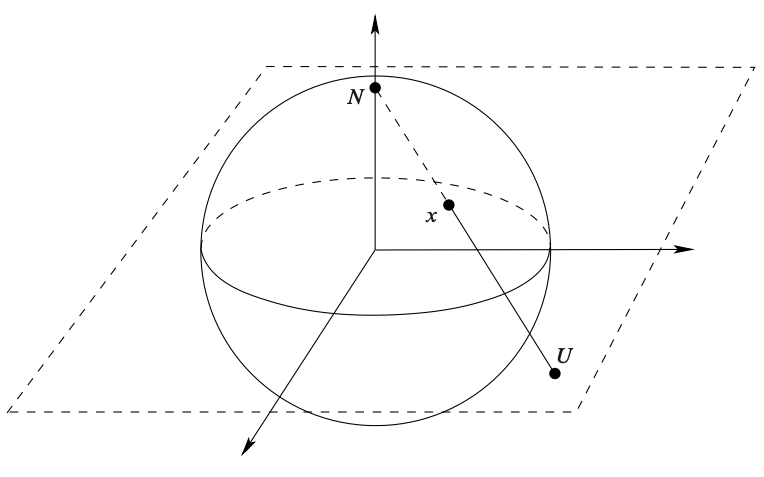
\includegraphics[width=1.2\textwidth]{figs/stereo.png}
	\end{center}
	\caption{Stereographic projection}
\end{marginfigure}the converse it suffices to show that the inverse image of a single open interval is open,
 because the inverse image of a union of sets is the union of the inverse images. So let $I = (c,d)$,
 and let $p\in f^{-1}(I)$ so that $f(p)\in I$. Choose $\epsilon=\min\br{f(p)-c,d- f(p)}$. As $f$ is C2, there
 exists a $\delta$ such that the open interval $(p - \delta, p + \delta)$ is in $f^{-1}(I)$. Therefore $f^{-1}(I)$
  is the union of open sets, which shows that $f$ is C1.\\\\
  To extend into multiple dimensions just use an appropriate chart $\varphi$, compose
 $f \circ \varphi^{-1}: \R^n \to \R$ to follow the proof above. Also $\epsilon$ and $\delta$
  become vectors, and change $\abs{\cdot}$ to $\norm{\cdot}$.


\begin{example}\label{b1e3}
	Given a topological space $X$ and a subset $S \subseteq X$, define the
	\tb{induced topology} on $S$ to be the topology in which the open sets are
	of the form $U \cap S$, where $U$ is open in $X$. Let $S^n$, the
	\tb{n-sphere}, be the unit sphere in $\R^{n+1}$:
	$$
		S^n = \br{\vec{x} \in \R^{n+1} | \sum_{i=1}^{n+1}\p{x^i}^2=1}
		\marginnote{Here superscript shows contravariant
vector components, not exponentiation.}
	$$
	Show that $S^n \subset \R^{n+1}$ with its induced topology is a manifold.
\end{example}
\sol Let $N = (0,\dots,0,1)$ denote the north pole in $S^n$, and define the
\tb{stereographic projection} to be the map $\sigma:S^n\setminus\br{N}\to\R^n$
that sends a point $x \in S^n\setminus\br{N}$ to the point $u\in\R^n$ chosen so that
$U=\p{u, 0}$ is the point in $\R^{n+1}$ where the line through $N$ and $x$ meets the
subspace where $x^{n+1}=0.$
To find a formula for $\sigma$, we note that $u=\sigma(x)$
is characterized by the vector equation $U-N=\lambda(x-N)$ for some real number $\lambda$.
This leads to the system of equations:
$$
\begin{aligned}
	u^i &= \lambda x^i, \qquad i=1,\dots,n\\
	-1 &= \lambda(x^{n+1} - 1) \marginnote{(1)}
\end{aligned}
$$
Solve the last equation for $\lambda$ and substitute into the other equations to obtain:
$$
	\sigma(x^1,\dots,x^{n+1}) = \frac{(x^1,\dots,x^{n+1})}{1-x^{n+1}}
$$
Its inverse can be found by solving (1) to get:
$$
	x^i = \frac{u^i}{\lambda}, \qquad x^{n+1} = \frac{\lambda-1}{\lambda}
	\marginnote{(2)}
$$
The point $x=\sigma^{-1}(u)$ is characterized by these equations together with the
fact that $x$ is on the unit sphere. Substituting (2) into $\norm{x}^2=1$ and solving
for $\lambda$ gives:
$$
	\lambda=\frac{\norm{u}^2+1}{2}
$$
and inserting this back into (2) yields:
$$
	\sigma^{-1}(u^1,\dots,u^n)=\frac{(2u^1,\dots,2u^n,\norm{u}^2-1)}{\norm{u}^2+1}
$$
Because this is a continuous inverse for $\sigma$, it follows that $S^n\setminus\br{N}$ is homeomorphic to $\R^n$, making $S^n$ an $n$-manifold. This procedure provides a Euclidean neighborhood of
every point of $S^n$ except $N$, and the analogous projection from the south pole
works in a neighborhood of $N$.


\begin{example}\label{b1e4}
	Show that if $M$ is a manifold and $U$ is an open subset of $M$, then $U$ with
	its induced topology is a manifold.
\end{example}
\sol Say $U$ is a disjoint union of open sets $U_i$.
If $A=\br{(U_i,\varphi_i)}$ is an atlas for $M$,
then $A^\prime=\br{(U_i \cap U,\varphi_i^\prime)}$ is an atlas for $U$, where
$\varphi_i^\prime = \varphi|_{U_i \cap U}$.\\\\
Since intersection of open sets is open, $U_i \cap U$ is open, and the transition functions
$\varphi_i^\prime \circ (\varphi_j^\prime)^{-1}$ will be smooth as well for any charts
$(U_i \cap U,\varphi_i^\prime)$ and $(U_j \cap U,\varphi_j^\prime)$ in $A^\prime$.
Hence $U$ is a manifold. This is not much of a reach because by definition if $U$ is an open \emph{cover}
of $M$ with an atlas $A$ then $M$ is a manifold.


\begin{definition}
	\tb{Paracompactness:} 
	A topological space $X$ is said to be compact if every open cover of $X$ has a finite subcover. A space $X$ is said to be paracompact if every open cover of $X$ admits a locally finite open refinement.\mn{A collection $\cal{A}$ of subsets of $X$ is said 
		 to be locally finite if each point of $X$ has a neighborhood that intersects
		  at most finitely many of the sets in $\cal{A}$. Given a cover $\cal{A}$ of $X$, another 
		  cover $\cal{B}$ is called a refinement of $\cal{A}$ if for each $B \in\cal{B}$ there exists some
		   $A \in\cal{A}$ such that $B \subseteq A$. It is an open refinement if each $B \in\cal{B}$ is an open subset
			of $X$. (Note that every subcover of $\cal{A}$ is a refinement of $\cal{A}$; but a refinement
			 is not in general a subcover, because a refinement does not need to be
			  composed of sets that are elements of $\cal{A}$.)}
\end{definition}


\begin{definition}
	\tb{Hausdorff spaces:} Consider a set $\br{p_0}$ containing only one point.
	Given $p \ne p_0$, the Hausdorff property says that there exist disjoint 
	neighborhoods $U$ of $p$ and $V$ of $p_0$.
\end{definition}


\begin{definition}
	\tb{Second countable spaces:} We say that $X$ is first countable
	if there exists a countable neighborhood basis at each point $p$, i.e, a countable collection
	of nested neighborhoods around $p$. If $X$ is second countable:
	\begin{itemize}
		\item $X$ is first countable.
		\item $X$ contains a countable dense subset.
		\item Every open cover of $X$ has a countable subcover.
	\end{itemize}
\end{definition}


\begin{example}\label{b1e5}
	Given topological spaces $X$ and $Y$, we give $X \cross Y$ the \tb{product topology}
	in which a set is open if and only if it is a union of sets of the form $U \cross V$,
	where $U$ is open in $X$ and $V$ is open in $Y$. Show that if $M$ is an $m$-dimensional
	manifold and $N$ is an $N$-dimensional
	manifold, $M \cross N$ is an $(m+n)$-dimensional manifold.
\end{example}
\sol To make it simpler let's assume that the product space is Hausdorff and second
countable, so only the locally Euclidean property needs to be checked. Given any point
$p = (p_M, p_N) \in M \cross N$, there exist open sets $U, V$ within neighborhoods of $p_M, p_N$
that get sent by homeomorphisms $\varphi_M, \varphi_N$ to an open subset of $\R^m$ and $\R^n$ respectively.
Why? Because $M \cross N$ is a manifold.\\\\
Now, we propose that a product of continuous
maps is continuous, and a product of homeomorphisms is a homeomorphism. So the product map
$\varphi_M \times \varphi_N$ is a homeomorphism from a neighborhood of $p$ to an open subset
of $\R^m \cross \R^n \cong \R^{m+n}$. In general, $M_1 \cross \dots \cross M_k$ is a $(d_1 + \dots + d_k)$-dimensional manifold.


\begin{example}
	Given topological spaces $X$ and $Y$, we give $X \cup Y$ the \tb{disjoint union topology}
	in which a set is open if and only if it is the union of an open subset of $X$
	and an open subset of $Y$. Show that if $M$ and $N$ are $n$-dimensional manifolds
	the disjoint union $M \cup N$ is an $n$-dimensional manifold.
\end{example}
\sol Let $A = \br{(U_i, \varphi_i)}$ be an atlas of $M$ and $B = \br{(V_j, \psi_i)}$ be an atlas for $N$.
Then $A \cup B$ is trivially an atlas for $X \cup Y$ since $U_i \cap V_j = \emptyset$
for all charts, the transition functions only exist on $M$ or $N$ seperately, and are smooth by definition.
Thus $M \cup N$ is an $n$-dimensional manifold.




\newpage
\section{Vector Fields}\label{b1c3}



\begin{example}
	Show that $v+w$ and $gw \in \text{Vect}(M)$.
\end{example}
\sol We first show $v+w$ satisfies the properties of a vector field:\mn{
	A \tb{vector field} $v$ on $M$ is defined to be a function from $C^\infty(M)$ to $C^\infty(M)$ satisfying the following three properties:
	\begin{enumerate}
		\item $v(f+g)=v(f)+v(g)$
		\item $v(\alpha f)=\alpha v(f)$
		\item $v(fg)=v(f)g+fv(g)$
	\end{enumerate}}
	$$
	\begin{aligned}
		(v+w)(f+g)&=v(f+g)+w(f+g)\\
		&=v(f)+v(g)+w(f)+w(g)\\
		&=(v+w)(f)+(v+w)(g)\\\\
		(v+w)(\alpha f)&=v(\alpha f)+w(\alpha f)\\
		&=\alpha v(f)+\alpha w(f)\\
		&=\alpha (v+w)(f)\\\\
		(v+w)(fg)&=v(fg)+w(fg)\\
		&=v(f)g+fv(g)+w(f)g+fw(g)\\
		&=(v+w)(f)g+f(v+w)(g)
	\end{aligned}
	$$
	Similarly we can show that:
	$$
	\begin{aligned}
		(gw)(f+g)&=(gw)(f)+(gw)(g)\\
		(gw)(\alpha f)&=\alpha (gw)(f)\\
		(gw)(fg)&=(gw)(f)g+(gw)v(g)
	\end{aligned}
	$$

\begin{example}\label{b1e8}
	Show that the following rules for all $v,w \in \text{Vect}(M)$ and
	$f, g \in C^\infty(M)$:
	$$
	\begin{aligned}
		f(v+w) &= fv + fw\\
		(f+g)v &= fv+gv\\
		(fg)v &= f(gv)\\
		1v &= v
	\end{aligned}
	$$
	(Here `$1$' denotes the constant function equal to $1$ on all of $M$.). 
	Mathematically, we summarize these rules by saying that $\text{Vect}(M)$ is 
	a \tb{module} over $C^\infty(M)$.
\end{example}
\sol Applying above rules:
$$
\begin{aligned}
	[f(v+w)](g) &= fv(g) + fw(g) = [fv + fw](g)\\
	[(f+g)v](h) &= (f+g)v(h)=[fv+gv](h)\marginnote{$\forall h \in C^\infty(M)$}\\
	[(fg)v](h) &= (fg)v(h)=[f(gv)](h)\marginnote{$\forall h \in C^\infty(M)$}\\
	[1v](f) &= 1\cdot v(f)=v(f)
\end{aligned}
$$


\begin{example}\label{b1e9}
	Show that if $v^\mu\partial_\mu = 0$, that is, \marginnote{In general, we have $$v=v^\mu\partial_\mu = v^1\partial_1 + \cdots + v^n\partial_n$$}
	$v^\mu\partial_\mu f = 0$ for all $f \in C^\infty(\R^n)$, we must have $v^\mu = 0$ for all $\mu$.
\end{example}
\sol Without loss of generality choose $f = x^i$.
$$
\begin{aligned}
	v^\mu \partial_\mu f &= v^\mu \partial_\mu x^i\\
	&= v^\mu \delta_\mu^i\marginnote{Kronecker delta}\\
	&= v^i = v^\mu = 0\marginnote{Just changing labels $i \to \mu$}
\end{aligned}
$$


\begin{example}\label{b1e10}
	Let $v,w \in \text{Vect}(M)$. Show that $v = w$ if and only if $v_p = w_p$
	for all $p \in M$.
\end{example}
\sol Proving the implication $\Rightarrow$. Let $v=w$:
$$
	\begin{aligned}
		(v-w) &= 0\\
		(v-w)(f) &= 0 \marginnote{$\forall f \in C^\infty(M)$}\\
		(v-w)(f)(p) &= 0 \marginnote{$\forall p \in M$}\\
		v_p &= w_p
	\end{aligned}
$$
Proving the converse $\Leftarrow$, amounts to letting $v_p = w_p$ and following the above steps in reverse.


\begin{definition}
\tb{Vector space axioms:}\\\\
A \tb{vector space} over a field $\F$ is the triple $(V, +, \cdot)$ where:
\begin{itemize}
	\item $V$ is a set
	\item $+$ is the addition map, $+:V \cross V \to V$
	\item $\cdot$ is the s-multiplication map, $\cdot:\F \cross V \to V$
\end{itemize}
satisfying these properties for all $u,v,w \in V$ and $a,b \in \F$:
\begin{enumerate}
	\item Commutative w.r.t $+$; $u+v = v+u$
	\item Associative w.r.t $+$; $(u+v)+w = u+(v+w)$
	\item $\exists$ neutral element w.r.t $+$; $e+u = u$ 
	\item $\exists$ inverse element w.r.t $+$; $u+u^{-1}=u^{-1}+u=e$
	\item Commutative w.r.t $\cdot$; $a\cdot b = b\cdot a$
	\item Associative w.r.t $\cdot$: $(a\cdot b)\cdot u = a\cdot (b\cdot u)$
	\item Distributive over $\F$; $a \cdot(u+v) = a \cdot u+a \cdot v$
	\item Distributive over $V$; $u \cdot(a+b) = a \cdot u+a \cdot v$
	\item Unitary w.r.t $\cdot$; $1\cdot u = u$
\end{enumerate}
An \tb{algebra} over a field is a vector space equipped with a bilinear product.
\end{definition}


\begin{example}
	Show that $T_pM$ is a vector space over the real numbers.
\end{example}
\sol While it is true that around a point $p$ on an $n$-manifold $M$ it looks like $\R^n$ (locally Euclidean property), that is not enough to show that $T_pM$ is a vector space over the reals. Formally, we should show that the tangent vectors $v_p$ satisfy the axioms of a vector space, where $V = T_pM$ and $\F = \R^n$ which we skip here.


\begin{example}\label{b1e12}
	Check that $\gamma^\prime(t) \in T_{\gamma(t)}M$ using the definitions.
\end{example}
\sol We have that
$$
	\gamma^\prime(t): f \mapsto \frac{d}{dt}f(\gamma(t))
$$
We check that the usual three properties of a vector space apply:
$$
\begin{aligned}
	\gamma^\prime(t)(f+g) &= \frac{d}{dt}(f+g)(\gamma(t)) = \frac{d}{dt}(f(\gamma(t))) + \frac{d}{dt}(g(\gamma(t))) = \gamma^\prime(t)(f) + \gamma^\prime(t)(g)\\
	\gamma^\prime(t)(\alpha f) &= \frac{d}{dt}(\alpha f)(\gamma(t)) = \alpha \gamma^\prime(t)(f)\\
	\gamma^\prime(t)(fg) &= \frac{d}{dt}(fg)(\gamma(t))\\
	&= \frac{d}{dt}\sparen*{f(\gamma(t)) \cdot g(\gamma(t))}\\
	&= \gamma^\prime(t)(f)g(\gamma(t)) + f(\gamma(t))\gamma^\prime(t)(g)
\end{aligned}
$$
The tangent vector $\gamma^\prime(t)$ thus belongs to the tangent space $T_{\gamma(t)}M$.


\begin{example}
	Let $\phi:\R\to\R$ be given by $\phi(t)=e^t$. Let $x$ be the usual coordinate function on $\R$.
	Show that $\phi^*x=e^x$.
\end{example}
\sol The map is defined as
$$
	\phi: t \mapsto e^t
$$
So $\phi^*x = x \circ \phi = e^x$.


\begin{example}\label{b1e14}
	Let $\phi:\R^2\to\R^2$ be rotation counterclockwise by an angle $\theta$.
	Let $x, y$ be the usual coordinate functions on $\R^2$. Show that
	$$
		\begin{aligned}
			\phi^*x &= (\cos\theta)x - (\sin\theta)y\\
			\phi^*y &= (\sin\theta)x + (\cos\theta)y.
		\end{aligned}
	$$
\end{example}
\sol The rotation matrix is defined as
$$
\phi:\begin{pmatrix}
	x\\y
\end{pmatrix}\mapsto
\begin{pmatrix}
	\cos\theta&-\sin\theta\\
	\sin\theta& \cos\theta\\
\end{pmatrix}
\begin{pmatrix}
	x\\y
\end{pmatrix}
$$
$\phi^*x$ and $\phi^*y$ are just what the coordinates get mapped to by the above transformation.


\begin{example}
	Show that this definition of smoothness is consistent with the previous definitions
	of smooth functions $f:M\to \R$ and smooth curves $\gamma:\R \to M$.
\end{example}
\sol Recall the definition of smooth functions between manifolds:
\begin{center}
	$\phi:M\to N$ is smooth if $f \in C^\infty(N)$ implies that $\phi^*f\in C^\infty(M)$.
\end{center}
Proving our other two definitions of smoothness:
\begin{enumerate}
	\item A function $f:M\to\R$ is smooth if for all charts $\alpha$, $f \circ \varphi^{-1}_\alpha:\R^n\to\R$ is smooth.\\
	With $N=\R$, if $f \in C^\infty(\R)$ and $\phi \in C^\infty(M)$ then a composition of smooth maps $f \circ \phi \in C^\infty(M)$ and composing that with a chart inverse $f \circ \phi \circ \varphi^{-1}_\alpha$ are also smooth. 
	\item A curve $\gamma:\R \to N$ is smooth if $f(\gamma(t))$ depends smoothly on $t$ for any $f \in C^\infty(N)$\\
	With $M=\R$, if $f \in C^\infty(N)$, then $f \circ \gamma \in C^\infty(\R)$ is smooth means $\gamma^*f$ is smooth.
\end{enumerate}



\begin{example}
	Prove that $(\phi \circ \gamma)^\prime(t) = \phi_*(\gamma^\prime(t))$.
\end{example}
\sol Applying to a smooth function $f \in C^\infty(M)$:
$$
\begin{aligned}
	\marginnote{Using Ex \ref{b1e12}}(\phi \circ \gamma)^\prime(t)(f) &= \frac{d}{dt}f((\phi \circ \gamma)(t))\\
	&= \frac{d}{dt}(f \circ \phi \circ \gamma)(t)\\
	&= \frac{d}{dt}(f \circ \phi)(\gamma(t))\\
	&= (\gamma^\prime(t))(f \circ \phi)\\
	&= (\gamma^\prime(t))(\phi^* f)\\
	&= \phi_*(\gamma^\prime(t))(f)\\
	\Rightarrow (\phi \circ \gamma)^\prime(t) &= \phi_*(\gamma^\prime(t))
\end{aligned}
$$

\begin{example}
	Show that the pushforward operation
	$$
		\phi_*:T_pM\to T_{\phi(p)}N
	$$
	is linear.
\end{example}
\sol Checking linearity can be done in one swift calculation:\mn{
	Linearity basically means:
	$$
		f(\alpha u+\beta v) = \alpha f(u)+\beta f(v)
	$$
}
$$
	\begin{aligned}
		(\phi_*(\alpha u+\beta v))(f) &= (\alpha u+\beta v)(\phi^*f)\\
		&= \alpha u(\phi^*f)+\beta v(\phi^*f)\\
		&= \alpha (\phi_*u)(f)+\beta (\phi_*v)(f)\\
		&= (\alpha (\phi_*u)+\beta (\phi_*v))(f)\\
	\end{aligned}
$$


\begin{example}\label{b1e18}
	Show that if $\phi:M\to N$ we can push forward a vector field\mn{
		Just remember that you can push \emph{vectors} forward by any smooth map but you can only push \emph{vector fields} forward by a diffeomorphism. So in this example $\phi$ must be a diffeomorphism.
	} $v$ on $M$ to obtain
	a vector field $\phi_*v$ on $N$ satisfying
	$$
	(\phi_*v)_q = \phi_*(v_p)
	$$
	whenever $\phi(p)=q$.
\end{example}
\sol When acting on points on the same manifold, the correct definition of pushforward is:\marginnote{Ref [1] Pg 98}
$$
	\begin{aligned}
		\ub{\phi^*[\ob{(\phi_*v)(f)}{\text{Acts on manifold $N$}}]}{\text{Acts on manifold $M$}} &= \ob{v(\phi^*f)}{\text{Acts on manifold $M$}}\\
		(\phi_*v)(f) &= v(\phi^*f) \circ \phi^{-1}\marginnote{(1)}
	\end{aligned}
$$

Applying to some $f \in C^\infty(N)$:
$$
	\begin{aligned}
		(\phi_*v)_q(f) &= (\phi_*v)(f)(q)\\
		&= v(\phi^*f)(\phi^{-1}(q))\marginnote{Applying (1)}\\
		&= v(\phi^*f)(p)\marginnote{$\phi(p)=q \Rightarrow \phi^{-1}(q)=p$}\\
		&= \phi_*v(f)(p)\\
		&= \phi_*v_p(f)\\
	\end{aligned}
$$


\begin{example}
	Let $\phi:\R^2\to\R^2$ be rotation counterclockwise by an angle $\theta$.
	Let $\partial_x, \partial_y$ be the coordinate vector fields on $\R^2$.
	Show that at any point of $\R^2$
	$$
		\begin{aligned}
			\phi^*\partial_x &= (\cos\theta)\partial_x + (\sin\theta)\partial_y\\
			\phi^*\partial_y &= -(\sin\theta)\partial_x + (\cos\theta)\partial_y.
		\end{aligned}
	$$
\end{example}
\sol Similar to Ex \ref{b1e14}, except applied to a vector of partial derivatives, i.e., the basis. The transformation $\phi$ is now called a \tb{Jacobian}.


\begin{example}
	Let $v$ be the vector field $x^2\partial_x + y\partial_y$ on $\R^2$. Calculate
	the integral curves $\gamma(t)$ and see which ones are defined for all $t$.
\end{example}
\sol The integral curves $\gamma(t) = (x(t),y(t))$, and velocity is $v = x^2\partial_x + y\partial_y$. This means we have $x^\prime = x^2, y^\prime = y$.\\\\
Setting initial conditions to $\gamma(0) = (x(0),y(0)) = (\alpha,\beta)$ and solving the DE for $(x(t),y(t))$ gives us:
$$
	x(t) = \frac{\alpha}{\alpha t - 1}, \qquad y(t)=\beta e^t
$$
If $\alpha \ne 0$, as soon as $t = \frac{1}{\alpha}$ we get a singularity. So $x(t)$ is well defined for $\alpha = 0$. However, $\beta$ can be chosen at will, making $y(t)$ well defined for all $t$.\\\\
So the solutions are $\gamma(t) = (0,\beta e^t)$ for any $\beta \in \R$.


\begin{example}
	Show that $\phi_0$ is the identity map $\id:X\to X$, and that for all $s,t\in\R$
	we have $\phi_t\circ\phi_s=\phi_{t+s}$.
\end{example}
\sol For $p \in M$ and $t \in \R$ denote $\phi_t(p) = \hat{p}$. This means that $\gamma_p(t) = \hat{p}$, where $\gamma_p$ is an integral curve of $v$ such that $\gamma_p(0)=p$.\\\\
Consider the curve $\beta$ defined by $\beta(s)=\gamma(s+t)$. Then $\beta$ is an integral curve of $v$ and $\beta(0)=\hat{p}$, that is $\beta=\gamma_{\hat{p}}$. Hence,
$$
\begin{aligned}
	\phi_s(\hat{p}) = \gamma_{\hat{p}}(s) = \beta(s) = \gamma_m(s+t) = \phi_{s+t}(p)\\
	\Longleftrightarrow \phi_s \circ \phi_t = \phi_{s+t}
\end{aligned}
$$
Since $\phi_0 = \id_M$ holds by the very definition of $\phi_t$, we obtain:
$$
\phi_{-t} \circ \phi_t = \id_M = \phi_t  \circ \phi_{-t}
$$
In particular, each $\phi_t$ is a diffeomorphism and $\phi_t^{-1} = \phi_{-t}$.


\begin{example}
	Consider the normalized vector fields in the $r$ and $\theta$ directions on the
	plane in polar coordinates (not defined at the origin):
	$$
		\begin{aligned}
			v &= \frac{x\partial_x+y\partial_y}{\sqrt{x^2+y^2}}\\
			w &= \frac{x\partial_y-y\partial_x}{\sqrt{x^2+y^2}}
		\end{aligned}
	$$
	Calculate $[v,w]$.
\end{example}
\sol For some $f \in C^\infty(\R^2)$, any vector field $\vartheta$ on $\R^2$ has the form
$$
\vartheta = f(x)\partial_x + f(y)\partial_y
$$
Since $x = r\cos\theta$, $y=r\sin\theta$, differentiating w.r.t $r$ and $\theta$ gives
$$
	\begin{aligned}
		\partial_r\vartheta &= \cos\theta\partial_xf + \sin\theta\partial_yf\\
		\partial_\theta \vartheta &= -r\sin\theta\partial_xf + r\cos\theta\partial_yf
	\end{aligned}
$$
we get $v=\partial_r$ and $w=\partial_\theta/r$. Calculating Lie bracket:
$$
	\begin{aligned}
		[v,w] &= vw-wv\\
		&= \partial_r(\frac{\partial_\theta}{r})-\partial_\theta/r(\partial_r)\\
		&= -\frac{\partial_\theta}{r^2}\ub{+\frac{\partial_r\partial_\theta}{r}-\frac{\partial_\theta\partial_r}{r}}{\text{Cancel}}\\
		&= -\frac{\partial_\theta}{r^2}\marginnote{Ordinary mixed partial derivatives commute}\\
		&= -\frac{w}{r}
	\end{aligned}
$$


\begin{example}\label{b1e23}
	Check the equation above.\mn{Check errata as well!}
\end{example}
\sol The equation to check is that for any $f \in C^\infty(M)$:
$$
	[v,w](f)(p) = \frac{\partial^2}{\partial t\partial s}f(\psi_s(\phi_t(p))) - f(\phi_t(\psi_s(p)))\Big|_{s=t=0}
$$
which measures how flows $\phi_t,\psi_s$ generated by vector fields $v,w$ fail to commute.\\\\
Starting at $p$, evaluating $f$ and applying $[v,w]$:
$$
\begin{aligned}
	[v,w](f)(p) &= v(w(f))(p) - w(v(f))(p)\\
	&= \pd{}{t} (w(f))(\phi_t(p))|_{t=0} - \pd{}{s} (v(f))(\psi_s(p))|_{s=0}\\
	&= \pd{}{t} \p*{ \pd{}{s} f(\psi_s(\phi_t(p)))\Big|_{s=0}}\Big|_{t=0} - \pd{}{s} \p*{ \pd{}{t} f(\phi_t(\psi_s(p)))\Big|_{t=0}}\Big|_{s=0}\marginnote{Applying partial derivative to make sure we differentiate w.r.t the right time parameter: $v \to t, w \to s$}\\
	&= \frac{\partial^2}{\partial t\partial s}f(\psi_s(\phi_t(p))) - f(\phi_t(\psi_s(p)))\Big|_{s=t=0}
\end{aligned}
$$



\begin{example}\label{b1e24}
	Show that for all vector fields $u,v,w$ on a manifold, and all real numbers 
	$\alpha$ and $\beta$, we have:
	\begin{enumerate}
		\item $[v,w]=-[w,v]$
		\item $[u,\alpha v+\beta w]=\alpha[u,v]+\beta[u,w]$
		\item \text{The \tb{Jacobi identity}:} $[u,[v,w]] + [v,[w,u]] + [w,[u,v]] = 0$.
	\end{enumerate}
\end{example}
\sol Proofs:
\begin{enumerate}
	\item $[v,w] = -(wv-vw) = -[w,v]$
	\item $$\begin{aligned}
		[u,\alpha v+\beta w] &= u(\alpha v+\beta w)-(\alpha v+\beta w)u\\
		&= \ob{\alpha uv}{}+\ub{\beta uw}{} \ob{- \alpha vu}{}\ub{-\beta wu}{}\marginnote{Grouping like terms}\\
		&= \alpha[u,v]+\beta[u,w]
	\end{aligned}$$
	\item $$\begin{aligned}
		&[u,[v,w]] + [v,[w,u]] + [w,[u,v]]\\
		&= u[v,w]-[v,w]u + v[w,u]-[w,u]v + w[u,v]-[u,v]w\\
		&= uvw-uwv-vwu-wvu+vwu-vuw-wuv+uwv+wuv-wvu-uvw+vuw\\
		&= \cancelto{1}{uvw}-\cancelto{2}{uwv}-\cancelto{3}{vwu}-\cancelto{4}{wvu}+\cancelto{3}{vwu}-\cancelto{5}{vuw}-\cancelto{6}{wuv}+\cancelto{2}{uwv}+\cancelto{6}{wuv}-\cancelto{4}{wvu}-\cancelto{1}{uvw}+\cancelto{5}{vuw}\\
		&= 0
	\end{aligned}$$
\end{enumerate}



\newpage
\section{Differential Forms}\label{b1c4}
% Using word wrap (option + Z) on VS Code from here on out



\begin{example}
	Show that $\omega + \mu$ and $fw$ are really 1-forms, i.e, show linearity over $C^\infty(M)$
\end{example}
\sol Here
$$
\begin{aligned}
	f,g,h &\in C^\infty(M)\\
	\omega, \mu &\in \Omega^1(M)\\
	\text{and} \quad v, w &\in \text{Vect}(M)
\end{aligned}
$$
Proving linearity:
$$
\begin{aligned}
	(\omega + \mu)(gv+hw) &= \omega gv + \omega hw + \mu gv + \mu hw\\
	&= g(\omega + \mu)(v+w) + h(\omega + \mu)(v+w)\\
	f\omega(gv+hw) &= f\omega(gv) + f\omega(hw)\\
	&= g(f\omega)(v) + h(f\omega)(w)
\end{aligned}
$$


\begin{example}
	Show that $\Omega^1(M)$ is a module over $C^\infty(M)$ (see the definition in Ex \ref{b1e8})
\end{example}
\sol Follows from Ex \ref{b1e8}, for all $\omega, \mu \in \Omega^1(M)$ and $f,g,h \in C^\infty(M)$:
$$
\begin{aligned}
	[f(\omega+\mu)](g) &= f\omega(g) + f\mu(g) = [f\omega + f\mu](g)\\
	[(f+g)\omega](h) &= (f+g)\omega(h)=[f\omega+g\omega](h)\\
	[(fg)\omega](h) &= (fg)\omega(h)=[f(g\omega)](h)\\
	[1\omega](f) &= 1\cdot \omega(f)=\omega(f)
\end{aligned}
$$


\begin{example}
	Show that
	$$
	\begin{aligned}
		d(f+g) &= df+dg\\
		d(\alpha f) &= \alpha\: df\\
		(f+g)dh &= f\:dh+g\:dh\\
		d(fg) &= f\:dg+g\:df
	\end{aligned}
	$$
	for any $f,g,h \in C^\infty(M)$ and any $\alpha \in \R$.
\end{example}
\sol First three properties follow from linearity. So we check the Leibniz law for $v \in \text{Vect}(M)$:
$$
	\begin{aligned}
		d(fg)(v) &= v(fg)\\
		&= fv(g) + gv(f)\\
		&= f\:dg(v) + g\:df(v)\\
	\end{aligned}
$$


\begin{example}\label{b1e28}
	Suppose $f(x^1,\dots,x^n)$ is a function on $\R^n$. Show that
	$$
		df=\partial_\mu f\: dx^\mu
	$$
\end{example}
\sol Applying the differential on some $v \in \text{Vect}(\R^n)$:\marginnote{As $\br{\partial_\mu}$ form a basis:$$v = v^\mu\partial_\mu$$
}
$$
	df(v) = v(f) = v^\mu\partial_\mu f
$$
On the other hand
$$
\begin{aligned}
	\partial_\mu f\: dx^\mu(v) &= \partial_\mu f dx^\mu\\
	&= v^\nu\partial_\mu f\partial_\nu x^\mu\\
	&= v^\nu\partial_\mu f\delta_\nu^\mu\\
	&= v^\mu\partial_\mu f\\
\end{aligned}
$$
This proves $df=\partial_\mu f\: dx^\mu$.


\begin{example}
	Show that the 1-forms $\br{dx^\mu}$ are linearly independent, i.e., if
	$$
		\omega = \omega_\mu\: dx^\mu = 0
	$$
	then all the functions $\omega_\mu$ are zero.
\end{example}
\sol Again considering a test vector $v$:
$$
\begin{aligned}
	\omega(v) &= \omega_\mu dx^\mu(v)\\
	&= \omega_\mu v(x^\mu)\\
	&= v^\nu \omega_\mu \delta^\mu_\nu\\
	&= v^\nu \omega_\nu
\end{aligned}
$$
And just like Ex \ref{b1e9}, we can show that $\omega = 0 \Leftrightarrow \omega_\mu = 0$.


\begin{example}\label{b1e30}
	For the mathematically inclined: show that the $\omega_p$ is really well-defined by the formula above. That is, show that $\omega(v)(p)$ really depends only on $v_p$, not on the values of $v$ at other points. Also, show that a 1-form is determined by its values at points. In other words, if $\omega,\nu$ are two 1-forms on $M$ with $\omega_p=\nu_p$ for every point $p \in M$, then $\omega=\nu$.
\end{example}
\sol TODO first part.\\
We know that if $\omega_p=\nu_p$ for all $p \in M$, then using Ex \ref{b1e10} $\omega_p(v_p)=\nu_p(v_p)$ for some $v_p \in T_pM$. So straightforwardly $\omega(v)(p)=\nu(v)(p) \Rightarrow \omega = \nu$.


\begin{example}\label{b1e31}
	Show that the dual\mn{The dual of a linear map $f:V \to W$ is defined by $$(f^*\omega)(v)=\omega(f(v))$$ where $f^*:W^* \to V^*$.} of the identity map on a vector space $V$ is the identity map on $V^*$. Suppose that we have linear maps $F:V\to W$ and $G:W\to X$. Show that $(gf)^* = f^*g^*$.
\end{example}
\sol Let $\omega: V \to \R$ and $v \in V$. We have to prove $\id_{V^*}:V^*\to V^*$ is the identity map on $V^*$. 
$$
	(\id_{V^*}\omega)(v) = \omega(\id_V(v)) = \omega(v) \Rightarrow \id_{V^*}\omega = \omega
$$
Moreover,
$$
\begin{aligned}
	((gf)^*\omega)(v) &= (\omega)(g(f(v)))\\
	&= (g^*\omega)(f(v))\\
	&= ((f^*g^*)\omega)(v)\\
	& \Rightarrow (gf)^* = (f^*g^*)
\end{aligned}
$$

\begin{example}
	Show that the pullback of 1-forms defined by the formula above\mn{Given a 1-form $\omega$ on $N$, we get a 1-form $\phi^*\omega$ on $M$ defined by $$(\phi^*\omega)_p=\phi^*(\omega_q)$$ where $\phi(p)=q$} really exists and is unique.
\end{example}
\sol Proof of existence is very similar to the result in Ex \ref{b1e18}.
Proof of uniqueness comes from the result in Ex \ref{b1e30}.


\begin{example}
	Let $\phi:\R\to\R$ be given by $\phi(t)=\sin t$. Let $dx$ be the usual 1-form on $\R$. Show that $\phi^*\:dx = \cos t\:dt$.
	\mn{My guess is that this is what the author intended to ask, instead of $\phi_*\:dx = \cos t\:dt$, because pullback and the forms they act on are contravariant.}
\end{example}
\sol Using the fact that the exterior derivative is \tb{natural}:
$$
\begin{aligned}
	\phi^*(dx)_t &= d((\phi^*x)(t))\\
	&= d(x(\phi(t)))\marginnote{$(\phi^*x)(p) = x(\phi(p))$}\\
	&= d(x(\sin t))\marginnote{Treating $x(\cdot)$ as selecting point $t$ (?)}\\
	&= d(\sin t)_t\\
	&= (\cos t dt)_t\\
\end{aligned}
$$


\begin{example}
	Let $\phi:\R^2\to\R^2$ denote rotation counterclockwise by the angle $\theta$. Let $dx,dy$ be the usual basis of 1-forms on $\R^2$. Show that
	$$
		\begin{aligned}
			\phi^*dx &= \cos\theta\:dx - \sin\theta\:dy\\
			\phi^*dy &= \sin\theta\:dx + \cos\theta\:dy.
		\end{aligned}
	$$
\end{example}
\sol Using Ex \ref{b1e14}:
$$
\begin{aligned}
	\phi^*dx &= d(\phi^*x) = d(\cos\theta\:x-\sin\theta\:y) = \cos\theta\:dx - \sin\theta\:dy \:\textcolor{red}{- (\sin\theta\:x + \cos\theta\:y)d\theta}\\
	\phi^*dy &= d(\phi^*y) = d(\sin\theta\:x+\cos\theta\:y) = \sin\theta\:dx + \cos\theta\:dy \:\textcolor{red}{+ (\cos\theta\:x - \sin\theta\:y)d\theta}
\end{aligned}
$$
However I do get these additional terms marked in \textcolor{red}{red}.


\begin{example}
	Show that the coordinate 1-forms $dx^\mu$ really are the differentials of the local coordinates $x^\mu$ on $U$.
\end{example}
\sol Acting coordinate 1-forms on the coordinate vector fields associated to the local coordinates $x^\mu$:
$$dx^\mu(\partial_\nu) = \partial_\nu(x^\mu) = \delta^\mu_\nu\marginnote{$df(v)=vf$}$$
Now take the pullback of the coordinate 1-forms and act them on the pushforward of the coordinate vector fields:
$$(\phi^*dx^\mu)(\phi^{-1}_*\partial_\nu) = dx^\mu(\phi_*\phi^{-1}_*\partial_\nu) = dx^\mu(\partial_\nu)=\delta^\mu_\nu$$


\begin{example}
	In the situation above, show that
	$$
		dx^{\prime\nu} = \pd{x^{\prime\nu}}{x^\mu}dx^\mu.
	$$
	Show that for any 1-form $\omega$ on $\R^n$, writing
	$$
		\omega = \omega_\mu dx^\mu = \omega_\nu^\prime dx^{\prime\nu},
	$$
	your components $\omega^\prime_\nu$ are related to my components $\omega_\mu$ by
	$$
		\omega^\prime_\nu = \pd{x^{\mu}}{x^{\prime\nu}}\omega_\mu.
	$$
\end{example}
\sol Since 1-forms form a basis, $dx^{\prime\mu}=T^\nu_\mu dx^\mu$ for some linear transformation $T^\nu_\mu$. Acting on $\partial_\mu$, we get
$$
\begin{aligned}
	dx^{\prime\nu}\partial_\mu &= T_\lambda^\nu dx^\lambda \partial_\mu\\
	&= T_\lambda^\nu \delta_\mu^\lambda\\
	&= T_\mu^\nu\marginnote{(1)}
\end{aligned}
$$
but
$$
\begin{aligned}
	dx^{\prime\nu}\partial_\mu &= \partial_\mu x^{\prime\nu}\\
	&= \pd{x^{\prime\lambda}}{x^\mu} \partial_\lambda^\prime x^{\prime\nu}\\
	&= \pd{x^{\prime\lambda}}{x^\mu} \delta_\lambda^\nu\\
	&= \pd{x^{\prime\nu}}{x^\mu}\marginnote{(2)}
\end{aligned}
$$
Plugging (1) into (2), and (2) into the original transformation rule gives us:
$$
dx^{\prime\mu}=\pd{x^{\prime\nu}}{x^\mu} dx^\mu
$$ 
which allows us to write a 1-form $\omega = \omega_\mu dx^\mu$ in any basis.


\begin{example}\label{b1e37}
	Show this.\mn{Pulling back a coordinate 1-form looks like:$$\phi^*(dx^{\prime\nu})=\pd{x^{\prime\nu}}{x^\mu} dx^\mu$$}
\end{example}
\sol TODO
% We shall use the ``sloppy'' convention, where we treat the chart coordinate vector field with the same :
% $$
% \pd{x^{\prime\nu}}{x^\mu} := \pd{(\phi^*x^{\prime\nu})}{x^\mu}
% $$
% Acting on the coordinate vector field $\partial_\lambda$:
% $$
% \begin{aligned}
% 	\phi^*(dx^{\prime\nu})\partial_\lambda &= \phi^*\p*{\pd{x^{\prime\nu}}{x^\mu}dx^\mu}\partial_\lambda\\
% 	&= \pd{x^{\prime\nu}}{x^\mu}dx^\mu(\phi_*\partial_\lambda)\marginnote{Ex 36}\\
% 	&= \pd{x^{\prime\nu}}{x^\mu} dx^\mu(\partial_\lambda)\marginnote{Using convention}\\
% 	\Rightarrow \phi^*(dx^{\prime\nu}) &= \pd{x^{\prime\nu}}{x^\mu} dx^\mu
% \end{aligned}
% $$


\begin{example}
	Let
	$$
		e_\mu = T_\mu^\nu \partial_\nu,
	$$
	where $\partial_\nu$ are the coordinate vector fields associated to local coordinates on an open set $U$, and $T_\mu^\nu$ are functions on $U$. Show that the vector fields $e_\mu$ are a basis of vector fields on $U$ if and only if for each $p \in U$ the matrix $T_\mu^\nu(p)$ is invertible.
\end{example}
\sol We check $\Leftarrow$, the implication that $\{e_\mu\}$ is a basis supposing $T$ is invertible. Let $S = T^{-1}$:
$$
\begin{aligned}
	S_\mu^\lambda e_\lambda &= S_\mu^\lambda T_\lambda^\nu \partial_\nu\\
	&= \delta_\mu^\nu \partial_\nu\\
	&= \partial_\mu\\
\end{aligned}
$$
Any vector $u \in U$ can be expressed as
$$
	u = u^\mu \partial_\mu = u^\mu S_\mu^\lambda e_\lambda = u^{\prime\mu} e_\mu
$$
so ${E_\mu}$ is a basis ($\Leftarrow$). Similarly to check $\Rightarrow$, we must have that $S_\mu^\lambda T_\lambda^\nu = \delta_\mu^\nu$ which means $T$ is invertible.


\begin{example}
	Use the previous exercise to show that the dual basis exists and is unique.
\end{example}
\sol If $\{e_\mu\}$ is a basis of vector fields on $U$, we automatically get a \tb{dual basis} of 1-forms $\{f^\mu\}$ such that
$$
	f^\nu(e_\mu) = \delta_\mu^\nu = S_\mu^\lambda T_\lambda^\nu.
$$
Because $T$ exists, is invertible and therefore unique, so is the dual basis.\marginnote{Ref [5] Pg 80}


\begin{example}
	Let $e_\mu$ be a basis of vector fields on $U$ and let $f^\mu$ be the dual basis of 1-forms. Let
	$$
		e^\prime_\mu = T_\mu^\nu e_\nu
	$$
	be another basis of vector fields, and let $f^{\prime\mu}$ be the corresponding dual basis of 1-forms. Show that
	$$
		f^{\prime\mu} = (T^{-1})^\mu_\nu f^\nu.
	$$
	Show that if $v=v^\mu e_\mu = v^{\prime\mu} e^\prime_\mu$, then
	$$
		v^{\prime\mu} = (T^{-1})^\mu_\nu v^\nu,
	$$
	and that if $\omega=\omega_\mu f^\mu = \omega^\prime_\mu f^{\prime\mu}$ then
	$$
		\omega^\prime_\mu = T^\nu_\mu \omega_\nu.
	$$
\end{example}
\sol $T^{-1}$ is going to be the change of basis for the dual basis of 1-forms, as we can work out from the previous exercise. This applies to other contravariant objects like local coordinates (coordinate vector fields components) as well. However the covariant objects like coordinate vector fields and coordinate 1-form components are going to be transform with $T$.


\begin{example}
	Show that
	$$
		u \wedge v \wedge w = \det \begin{pmatrix}
			u_x&u_y&u_z\\v_x&v_y&v_z\\w_x&w_y&w_z
		\end{pmatrix}\:dx \wedge dy\wedge dz.
	$$
	Compare this to $\vec{u} \cdot (\vec{v} \times \vec{w})$.
\end{example}
\sol Simple algebra reveals 
$$\vec{u} \cdot (\vec{v} \times \vec{w}) = \det \begin{pmatrix}
	u_x&u_y&u_z\\v_x&v_y&v_z\\w_x&w_y&w_z
\end{pmatrix}$$


\begin{example}
	Show that if $a,b,c,d$ are four vectors in a 3-dimensional space then $a\wedge b\wedge c\wedge d = 0$.
\end{example}
\sol Let $\det(\cdot) \equiv \alpha$.
$$
\begin{aligned}
	a\wedge b\wedge c\wedge d &= a \wedge \alpha (dx \wedge dy\wedge dz)\\
	&= (a_xdx + a_ydy + a_zdz) \wedge \alpha (dx \wedge dy\wedge dz)\\
	&= \alpha a_xdx \wedge dx \wedge dy\wedge dz\\
	&+ \alpha a_ydy \wedge dx \wedge dy\wedge dz\\
	&+ \alpha a_zdz \wedge dx \wedge dy\wedge dz\\
	&= 0
\end{aligned}
$$
by antisymmetry: $x \wedge x = -(x \wedge x) = 0$.


\begin{example}
	Describe $\Lambda V$ if $V$ is 1-dimensional, 2-dimensional, or 4-dimensional.
\end{example}
\sol If $V$ is $n$-dimensional then $\Lambda V$ is the space of linear combinations of $p$-forms 
$$\omega = \omega_i (dx^{i_1} \wedge dx^{i_2} \wedge \dots \wedge dx^{i_p})$$
for all $p \le n$, and the $i_p$ are chosen from $1 \dots n$ without replacement. It has dimension $2^n$, the cardinality of the power set (set of all subsets).


\begin{example}
	Let $V$ be an $n$-dimensional vector space. Show that $\Lambda^p V$ is empty for $p > n$, and that for $0 \le p \le n$ the dimension of $\Lambda^p V$ is $n!/p!(n-p)!$.
\end{example}
\sol It checks out that
$$
\dim(\Lambda^p V) = ^n\!\!C_p = {n \choose p} = \frac{n!}{p!(n-p)!}
$$


\begin{example}
	Show that $\Lambda V$ is the direct sum of the subspaces $\Lambda^p V$:
	$$
		\Lambda V = \bigoplus \Lambda^p V,
	$$
	and that the dimension of $\Lambda V$ is $2^n$ if $V$ is $n$-dimensional.
\end{example}
\sol Every $v \in \Lambda V$ can be expressed as a linear combination of $v_p \in \Lambda^p V$, and by adding the dimension of each subspace
$$
\begin{aligned}
	\dim(\Lambda V) &= \sum_{p=0}^{n} \dim(\Lambda^p V)\\
	&= \sum_{p=0}^{n} {n \choose p}\\
	&= 2^n
\end{aligned}
$$


\begin{example}\label{b1e46}
	Given a vector space $V$, show that $\Lambda V$ is a \tb{graded commutative} or \tb{supercommutative} algebra, that is, if $\omega \in \Lambda^p V$ and $\mu \in \Lambda^q V$, then
	$$
		\omega \wedge \mu = (-1)^{pq} \mu \wedge \omega.
	$$
	Show that for any manifold $M$, $\Omega(M)$ is graded commutative.
\end{example}
\sol We have
$$
\begin{aligned}
	\omega \in \Lambda^p V &= \omega_1 \wedge \cdots \wedge \omega_p,\\
	\mu \in \Lambda^q V &= \mu_1 \wedge \cdots \wedge \mu_q
\end{aligned}
$$
So
$$
\begin{aligned}
	\omega \wedge \mu &= \omega_1 \wedge \cdots \wedge \omega_p \wedge \mu_1 \wedge \cdots \wedge \mu_q\\
	&= (-1)^p \mu_1 \wedge \omega_1 \wedge \cdots \wedge \omega_p \wedge \mu_2 \wedge \cdots \wedge \mu_q\marginnote{Each step incurs $p$ swaps}\\
	&= (-1)^{2p} \mu_1 \wedge \mu_2 \wedge \omega_1 \wedge \cdots \wedge \omega_p \wedge \mu_3 \wedge \cdots \wedge \mu_q\\
	&\:\;\vdots\\
	&= (-1)^{qp} \mu_1 \wedge \cdots \wedge \mu_q \wedge \omega_1 \wedge \cdots \wedge \omega_p\marginnote{$q$ total steps}\\
	&= (-1)^{pq} \mu \wedge \omega\\
\end{aligned}
$$


\begin{example}
	Show that differential forms are contravariant. That is, show that if $\phi:M\to N$ is a map from the manifold $M$ to the manifold $N$, there is a unique \tb{pullback} map
	$$
		\phi^*:\Omega(N)\to\Omega(M)
	$$
	agreeing with the usual pullback on 0-forms (functions) and 1-forms, and satisfying
	$$
		\begin{aligned}
			\phi^*(\alpha\omega) &= \alpha\phi^*\omega\\
			\phi^*(\omega+\mu) &= \phi^*\omega + \phi^*\mu\\
			\phi^*(\omega\wedge\mu) &= \phi^*\omega \wedge \phi^*\mu\\
		\end{aligned}
	$$
	for all $\omega,\mu \in \Omega(N)$ and $\alpha \in \R$.
\end{example}
\sol TODO


\begin{example}\label{b1e48}
	Compare how 1-forms and 2-forms on $\R^3$ transform under \tb{parity}. That is, let $P:\R^3\to\R^3$ be the map
	$$
		P(x,y,z)=(-x,-y,-z),
	$$
	known as the `parity transformation'. Note that $P$ maps right-handed bases to left-handed bases and vice versa. Compute $\phi^*(\omega)$ when $\omega$ is the 1-form $\omega_\mu dx^\mu$, and when it is the 2-form $\frac12 \omega_{\mu\nu}dx^\mu \wedge dx^\nu$.
\end{example}
\sol Assume $\phi^*$ is the pullpack by $P$. Consider the pullback of $dx^\mu$ acting on coordinate vector field $\partial_\nu$
$$
\begin{aligned}
	(\phi^*dx^\mu)\partial_\nu &= d(\phi^*x^\mu)\partial_\nu\\
	&= \partial_\nu(\phi^*x^\mu)\\
	&= \partial_\nu(x^\mu \circ \phi)\\
	&= -\delta_\nu^\mu\\
	&= -\partial_\nu x^\mu\\
	&= -dx^\mu\partial^\nu\\
	\Rightarrow \phi^*dx^\mu &= -dx^\mu
\end{aligned}
$$
If $\omega \in \Omega^1(\R^3)$
$$
\phi^*\omega = \phi^*(\omega_\mu dx^\mu) = -\omega
$$
If $\omega \in \Omega^2(\R^3)$
$$
	\begin{aligned}
		\phi^*\omega &= \phi^*\p*{\frac12 \omega_{\mu\nu} dx^\mu \wedge dx^\nu}\\
		&= \frac12 \omega_{\mu\nu}\phi^*\p*{dx^\mu \wedge dx^\nu}\\
		&= \frac12 \omega_{\mu\nu}\phi^*(dx^\mu) \wedge \phi^*(dx^\nu)\\
		&= \frac12 \omega_{\mu\nu}(-dx^\mu) \wedge (-dx^\nu)\\
		&= \omega
	\end{aligned}
$$
An important example is the $\vec{E}$ and $\vec{B}$ fields which transform differently under $P$.


\begin{example}\label{b1e49}
	Show that on $\R^n$ the exterior derivative of any 1-form is given by
	$$
		d(\omega_\mu dx^\mu) = \partial_\nu\omega_\mu dx^\nu \wedge dx^\mu.
	$$
\end{example}
\sol Since $\omega_\mu$ is a 0-form
$$
\begin{aligned}
	d(\omega_\mu dx^\mu) &= d(\omega_\mu \wedge dx^\mu)\marginnote{1-form = (0+1)-form}\\
	&= d\omega_\mu \wedge dx^\mu + \cancel{\omega_\mu \wedge d(dx^\mu)}\\
	&= \partial_\nu\omega_\mu dx^\nu \wedge dx^\mu\marginnote{Ref [3] Pg 363: If $f$ is a 0-form $$df=\partial_\mu f dx^\mu$$ }
\end{aligned}
$$



\newpage
\section{Rewriting Maxwell's Equations}\label{b1c5}




\begin{example}
	Show that any 2-form $F$ on $\R \cross S$ can be uniquely expressed as $B + E \wedge dt$ in such a way that for any local coordinates $x^i$ on $S$ we have $E=E_idx^i$ and $B=\frac12 B_{ij}dx^i\wedge dx^j$.
\end{example}
\sol Since $\R \cross S$ is a manifold, we have an atlas $\br{\varphi_\alpha}$ for all open sets $U_\alpha$ giving local coordinates $x^\mu = \varphi_\alpha(u)$ where $u \in U_\alpha$.\\\\
We have the space of 2-forms $\Omega^2(U_\alpha) = \Lambda^2 T_{(t,x^i)}^*(\R \cross S)$. Notice that $\br{dx^0 \wedge dx^i, dx^i \wedge dx^0, dx^i \wedge dx^j}$ span this space, and any $F \in \Omega^2(U_\alpha)$ is uniquely labelled by $i, j \in \br{1,2,3}$ where $t=x^0$. $F$ can be represented as:
$$
\begin{aligned}
	F &= \frac12 F_{\mu\nu} dx^\mu dx^\nu\marginnote{General form where $\mu,\nu \in \br{0,1,2,3}$}\\
	&= \frac12 (F_{0i} dt \wedge dx^i + F_{i0} dx^i \wedge dt + F_{ij} dx^i \wedge dx^j)\\
	&= \frac12 (2F_{i0} dx^i \wedge dt + F_{ij} dx^i \wedge dx^j)\marginnote{Since $F_{0i} = -F_{i0}$ by antisymmetry}\\
	&= \frac12 F_{ij} dx^i \wedge dx^j + F_{i0} dx^i \wedge dt\\
	&= \frac12 B_{ij} dx^i \wedge dx^j + E_{i} dx^i \wedge dt\marginnote{Relabelling $F_{ij} = B_{ij}$ and $F_{i0} = E_i$}\\
	&= B + E \wedge dt
\end{aligned}
$$


\begin{example}\label{b1e51}
	Show that for any form $\omega$ on $\R \cross S$ there is a unique way to write $d\omega=dt \wedge \partial_t\omega+d_S\omega$ such that for any local coordinates $x^i$ on $S$, writing $t=x^0$, we have
	$$
		\begin{aligned}
			d_S\omega &= \partial_i \omega_I dx^i \wedge dx^I,\\
			dt \wedge \partial_t\omega &= \partial_0 \omega_I dx^0 \wedge dx^I.
		\end{aligned}
	$$
\end{example}
\sol Since $\omega$ is any $p$-form we use multi-index $I$ to express $\omega = \omega_I dx^I$, giving us
$$
\begin{aligned}
	d\omega &= \partial_\mu \omega_I dx^\mu \wedge dx^I\\
	&= \partial_0 \omega_I dx^0 \wedge dx^I &&+ \partial_i \omega_I dx^i \wedge dx^I\\
	&= dt \wedge \partial_t\omega &&+ d_S\omega
\end{aligned}
$$


\begin{example}
	Use the nondegeneracy of the metric to show that the map from $V$ to $V^*$ given by
	$$
		v \mapsto g(v,\cdot)
	$$
	is an isomorphism, that is, one-to-one and onto.
\end{example}
\sol By nondegeneracy
$$
g(v,\cdot)-g(w,\cdot)=0 \Rightarrow v-w=0 \Rightarrow v=w
$$
so $g$ is injective or one-to-one.\\
We claim that $\omega=g(v,\cdot)$ for any $\omega \in V^*$ and some $v \in V$, which means
$$
\begin{aligned}
	\omega &= \omega_\mu f^\mu\marginnote{$\br{f^\mu}, \br{e_\mu}$ are bases for $V^*,V$ respectively}\\
	&= \omega_\mu g(e_\mu, \cdot)\\
	&= g(v, e_\mu) g(e_\mu, \cdot)\\
	&= g(v^\nu e_\nu, e_\mu) g(e_\mu, \cdot)\\
	&= v^\nu g(e_\nu, e_\mu) g(e_\mu, \cdot)
\end{aligned}
$$
Any covector in the dual space can be expressed in terms of vector components using the metric. Since the metric is nondegenerate, this mapping is surjective, and from above also bijective.


\begin{example}
	Let $v=v^\mu e_\mu$ be a vector field on a chart. Show that the corresponding 1-form $g(v,\cdot)$ is equal to $v_\mu f^\mu$, where $f^\mu$ is the dual basis of 1-forms and
	$$
		v_\nu = g_{\mu\nu}v^\mu.
	$$
\end{example}
\sol Using the same steps from previous exercise, except we leave $f^\nu$ as is and use the notation $g(e_\nu, e_\mu) = g_{\mu\nu}$
$$
\begin{aligned}
	\omega &= \omega_\nu f^\nu\marginnote{We switch $\mu \leftrightarrow \nu$ here}\\
	&= v^\mu g_{\mu\nu} f^\nu\\
	&= v_\nu f^\nu
\end{aligned}
$$
Where the metric tensor $g_{\mu\nu}$ is used in the usual way to raise/lower indices.


\begin{example}\label{b1e54}
	Let $\omega=\omega_\mu f^\mu$ be a 1-form on a chart. Show that the corresponding vector field is equal to $\omega^\nu e_\nu$, where
	$$
		\omega^\nu = g^{\mu\nu}\omega_\mu.
	$$
\end{example}
\sol Starting with vector field $v$
$$ 
\begin{aligned}
	v &= v^\nu e_\nu\\
	&= \omega_\mu g^{\mu\nu} e_\nu\\
	&= \omega^\mu e_\nu\\
\end{aligned}
$$
We change between vector and covector components using the inverse metric tensor $g^{\mu\nu}$.	\begin{marginfigure}
	\begin{center}
	  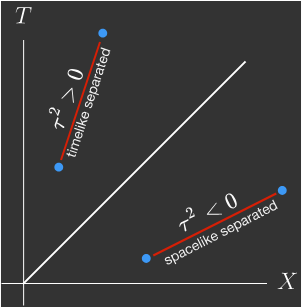
\includegraphics[width=1.2\textwidth]{figs/metric.png}
	\end{center}
	\caption{Spacetime events using the ``mostly minus'' or (1,3) metric. The text uses the (3,1) metric}
\end{marginfigure}	



\begin{definition}
	Different kinds of manifolds encountered in relativity:

	\begin{itemize}
		\item \tb{Riemannian} manifolds are the simplest with all positive definite lengths. They model smooth, curved surfaces like spheres or ellipsoids in higher dimensions.
		\item \tb{Semi-Riemannian} manifolds (also called pseudo-Riemannian) are a broader category including Riemannian and allowing more flexibility. Here, the inner product of tangent vectors can be positive definite (like Riemannian), negative definite, or zero.
		\item \tb{Lorentzian} manifolds are a specific type of semi-Riemannian crucial for general relativity. In Lorentzian manifolds, the signature is typically $(3,1)$ or $(1,3)$. This signature allows for the classification of tangent vectors into three categories:
		\begin{itemize}
			\item \tb{Timelike}: Represent directions corresponding to the passage of time.
			\item \tb{Spacelike}: Represent directions through space.
			\item \tb{Null}: These vectors have a $ds^2 = 0$ regardless of the signature of the metric and represent the direction of light propagation.
		\end{itemize}
	\end{itemize}
	The inclusion looks like:
	$$
	\tb{Lorentzian} \subset \tb{Riemannian} \subset \tb{Semi-Riemannian}
 	$$
\end{definition}


\begin{example}
	Let $\mu$ be the Minkowski metric on $\R^4$ as defined above. Show that its components in the standard basis are
	$$
		\eta_{\mu\nu} = \begin{pmatrix}
			-1&0&0&0\\0&1&0&0\\0&0&1&0\\0&0&0&1
		\end{pmatrix}
	$$
\end{example}
\sol For an orthonormal basis $\br{e_\mu}$, expand on the matrix form above:
$$
\eta_{\mu\nu} = \eta(e_\mu,e_\nu) = \begin{cases}
	-1& \quad\text{if $\mu=\nu=0$}\\
	1&  \quad\text{if $\mu=\nu=0$ and $1 \le \mu \le 3$}\\
	0&  \quad\text{otherwise}
\end{cases}
$$
Of course this depends on the signature of the metric, and switching between metrics makes $\eta \leftrightarrow -\eta$. This book uses the ``mostly plus'' metric.


\begin{example}
	Show that $g^\mu_\nu$ is equal to the Kronecker delta $\delta^\mu_\nu$, that is, $1$ if $\mu=\nu$ and $0$ otherwise. Note that here the order of indices does not matter, since $g^\mu_\nu = g^\nu_\mu$.
\end{example}
\sol Using the inverse metric to raise the index on the metric itself:
$$
g^\mu_\nu = g^{\mu\lambda} g_{\lambda\nu} = \delta^\mu_\nu
$$


\begin{example}\label{b1e57}
	Show that the inner product of $p$-forms is nondegenerate by supposing that $(e^1,\dots,e^n)$ is any orthonormal basis of 1-forms in some chart, with
	$$
		g(e^i,e^i) = \epsilon(i),
	$$
	where $\epsilon(i) = \pm 1$. Show that the $p$-fold wedge products
	$$
		e^{i_1} \wedge \cdots \wedge e^{i_p}
	$$
	form an orthonormal basis of $p$-forms with
	$$
		\ip{e^{i_1} \wedge \cdots \wedge e^{i_p}} = \epsilon(i_1)\cdots \epsilon(i_p).
	$$
\end{example}
\sol The inner product of two orthonormal basis 1-forms $e^i$ is $g^{ii} = \epsilon(i) = \pm 1$ by orthonormality and antisymmetry. If the inner product of two $p$-forms $\ip{\omega}{\mu} = 0\: \forall \mu$, then by nondegeneracy of the metric $\omega = 0$. In general $\ip{\omega}{\mu} = \det[g(e^i,f^j)]$, but in the specific case we are considering basis $p$-forms over some multi-index $i_1 \cdots i_p$ that inner products with itself as follows
$$
\ip{e^{i_1} \wedge \cdots \wedge e^{i_p}} = \det\begin{pmatrix}
	\epsilon(i_1)&&\\
	&\ddots&\\
	&&\epsilon(i_p)
\end{pmatrix} = \prod_{i=1}^{p} \epsilon(i_k) = \epsilon(i_1)\cdots \epsilon(i_p)
$$


\begin{example}\label{b1e58}
	Let $E = E_xdx + E_ydy + E_zdz$ be a 1-form on $\R^3$ with its Euclidean metric. Show that
	$$
		\ip{E} = E_x^2 + E_y^2 + E_z^2.
	$$
	Similarly, let
	$$
		B = B_xdy\wedge dz + B_ydz\wedge dx + B_zdx\wedge dy
	$$
	be a 2-form. Show that
	$$
		\ip{B} = B_x^2 + B_y^2 + B_z^2.
	$$
	In physics, the quantity
	$$
		\frac12\p{\ip{E}+\ip{B}}
	$$
	is called the \tb{energy density} of the electromagnetic field. The quantity
	$$
		\frac12\p{\ip{E}-\ip{B}}
	$$
	is called the \tb{Lagrangian} of the vacuum Maxwell's equations, which we discuss more in Sec \ref{b1e4}, in greater generality.
\end{example}
\sol Taking inner product of 1-form $E$:
$$
\begin{aligned}
	\ip{E} &= g^{ij} E_i E_j\\
	&= \delta^{ij} E_i E_j\\
	&= E_x^2 + E_y^2 + E_z^2
\end{aligned}
$$
From the previous exercise we can calculate the inner product of basis 2-forms as
$$
\ip{dx^i \wedge dx^j}{dx^k \wedge dx^l} = g(dx^i, dx^k)g(dx^j, dx^l) = \delta^{ik}\delta^{jl}\marginnote{This means cross terms will cancel out}
$$
Taking inner product of 2-form $B$:
$$
\begin{aligned}
	\ip{B} &= \ip{B}{B_xdy\wedge dz + B_ydz\wedge dx + B_zdx\wedge dy}\\
	&= B_x^2\ip{dy\wedge dz} + B_xB_y\ip{dy\wedge dz}{dz\wedge dx} + B_xB_z\ip{dy\wedge dz}{dx\wedge dy}\\
	&+ B_yB_x\ip{dz\wedge dx}{dy\wedge dz} + B_y^2\ip{dz\wedge dx} + B_yB_z\ip{dz\wedge dx}{dx\wedge dy}\\
	&+ B_zB_x\ip{dx\wedge dy}{dy\wedge dz} + B_zB_y\ip{dx\wedge dy}{dz\wedge dx} + B_z^2\ip{dx\wedge dy}\\
	&= B_x^2 + B_y^2 + B_z^2
\end{aligned}
$$


\begin{example}\label{b1e59}
	In $\R^4$ let $F$ be the 2-form given by $F=B+E\wedge dt$, where $E$ and $B$ are given by the formulas above. Using the Minkowski metric on $\R^4$, calculate $-\frac12 \ip{F}$ and relate it to the Lagrangian above.
\end{example}
\sol Taking inner product of 2-form $F$:
$$
\begin{aligned}
	-\frac12 \ip{F} &= -\frac12 (\ip{B+E\wedge dt})\\
	&= -\frac12 (\ip{B} + \ip{B}{E\wedge dt} + \ip{E\wedge dt}{B} + \ip{E\wedge dt})\marginnote{$B$ and $E\wedge dt$ are component-wise orthogonal}\\
	&= -\frac12 (\ip{B} + \cancel{\ip{B}{E\wedge dt} + \ip{E\wedge dt}{B}} + \ip{E\wedge dt})\\
	&= -\frac12 (\ip{B} + \ip{E\wedge dt})\marginnote{In the Minkowski metric:$$\begin{aligned}
		&\ip{E\wedge dt}\\ &= \ip{E}\ip{dt}\\ &= -\ip{E}
	\end{aligned}$$}\\
	&= -\frac12 (\ip{B} - \ip{E})\\
	&= \frac12 (\ip{E} - \ip{B})\\
\end{aligned}
$$


\begin{example}\label{b1e60}
	Show that any even permutation of a given basis has the same orientation, while any odd permutation has the opposite orientation.
\end{example}
\sol A permutation $\sigma$ is represented by its transposition matrix $T$, which is the same as the identity except columns (or rows) $i, j$ are swapped if basis elements $e_i, e_j$ are being swapped. This results in
$$
\det(T) = (-1)^{\text{sign}(\sigma)} = \begin{cases}
	1 \quad &\text{if $\sigma$ is an even permutation}\\
	-1 &\text{if $\sigma$ is an odd permutation}
\end{cases}
$$


\begin{example}
	Let $M$ be an oriented manifold. Show that we can cover $M$ with \tb{oriented charts} $\varphi:U_\alpha \to \R^n$, that is, charts such that the basis $dx^\mu$ of cotangent vectors on $\R^n$, pulled back to $U_\alpha$ by $\varphi_\alpha$, is positive oriented.
\end{example}
\sol For some $p \in U_\alpha$ we have an oriented chart $\varphi_\alpha:p \mapsto x^\mu(p)$ which gives us a basis $\br{dx^\mu}$ of the cotangent space $T_p^*M \simeq \R^n$. Pulling back a volume form $\omega$ using $\varphi^*_\alpha$ gives us
$$
\begin{aligned}
	\varphi^*_\alpha\omega &= \varphi^*_\alpha(dx^1 \wedge \cdots \wedge dx^n)\\
	&= \varphi^*_\alpha dx^1 \wedge \cdots \wedge \varphi^*_\alpha dx^n\\
	&= d\varphi^*_\alpha x^1 \wedge \cdots \wedge d\varphi^*_\alpha x^n
\end{aligned}
$$
which is a volume form corresponding to a basis on $U_\alpha$ that preserves its orientation at every point $p \in M$.


\begin{example}\label{b1e62}
	Given a diffeomorphism $\phi:M \to N$ from one oriented manifold to another, we say that $\phi$ is \tb{orientation-preserving} if the pullback of any right-handed basis of a cotangent space in $N$ is a right-handed basis of a cotangent space in $M$. Show that if we can cover $M$ with charts such that the transition functions $\varphi_\alpha \circ \varphi_\beta^{-1}$ are orientation-preserving, we can make $M$ into an oriented manifold by using the charts to transfer the standard orientation on $\R^n$ to an orientation on $M$.
\end{example}
\sol Let $\dim(M)=n$ and let $p \in U_\alpha, q \in U_\beta$ are $U_\alpha, U_\beta$ are overlapping open sets with charts $\varphi_\alpha:p\mapsto \br{x^{\mu}}, \varphi_\beta:q\mapsto \br{x^{\prime\nu}}$. Each chart admits volume forms
$$
\omega = dx^1 \wedge \cdots \wedge dx^n, \omega^\prime = dx^{\prime1} \wedge \cdots \wedge dx^{\prime n}
$$
On the overlap $U_\alpha \cap U_\beta$ we have
$$
\begin{aligned}
	(\varphi_\alpha \circ \varphi_\beta^{-1})^* dx^{\prime\nu} &= T_\mu^\nu dx^\mu\marginnote{Ex \ref{b1e37} shows a matrix representation of transformation on 1-forms is given by $$T_\mu^\nu = \pd{x^{\prime\nu}}{x^\mu}$$}\\
	\Rightarrow(\varphi_\alpha \circ \varphi_\beta^{-1})^* \omega^\prime &= (\varphi_\alpha \circ \varphi_\beta^{-1})^*(dx^{\prime1} \wedge \cdots \wedge dx^{\prime n})\\
	&= T_\mu^1 (dx^1 \wedge \cdots \wedge dx^n)\\
	&= T_\mu^1 dx^1 \wedge \cdots \wedge T_\mu^n dx^n\\
	&= \det(T)\:(dx^1 \wedge \cdots \wedge dx^n)\\
	&= \det(T)\:\omega
\end{aligned}
$$
and we know from Ex \ref{b1e60} that transpositions are orientation preserving.


\begin{example}\label{b1e63}
	Let $M$ be an oriented $n$-dimensional semi-Riemannian manifold and let $\br{e^\mu}$\mn{Correction from the text: index must be contravariant} be an oriented orthonormal basis of cotangent vectors at some point $p \in M$. Show that
	$$
		e^1 \wedge \cdots \wedge e^n = \vol_p
	$$
	where $\vol$ is the volume form associated to the metric on $M$, and $\vol_p$ is its value at $p$.
\end{example}
\sol The basis $\br{e^\mu}$ has to be some rescaling of the standard basis $\br{dx_\mu}$ that spans $T_p^*M$. Since the new basis remains orthonormal, the transformation is unitary (scaling constant is $1$), and we get the same volume form at $p$: $\vol_p$.


\begin{example}
	Show that if we define the Hodge star operator in a chart using this formula, it satisfies the property $\omega \wedge \star\mu = \ip{\omega}{\mu} \vol$. Use the result from Ex \ref{b1e63}.
\end{example}
\sol We have $\omega = \omega_I e^I$ and $\mu = \mu_J e^J$. By antisymmetry and Hodge duality\mn{The \tb{Hodge star operator} is $$\star:\Omega^p(M) \to \Omega^{n-p}(M)$$} we know $\omega \wedge \star\mu \ne 0$ implies the following:
\begin{itemize}
	\item They have the same multi-index: $I = J$
	\item They share the same basis: $e^I = e^J$
	\item They are simply rescalings of the same underlying volume form
\end{itemize}  
We then calculate
$$
\begin{aligned}
	\omega \wedge \star\mu &= \pm \omega_I \mu_J \delta^{IJ} e^{i_1} \wedge \cdots \wedge e^{i_p} \wedge e^{i_{p+1}} \cdots \wedge e^{i_n}\\
	&= \pm \omega_I \mu_J \delta^{IJ} e^{i_1} \wedge \cdots \wedge e^{i_n}\\
	&= \sign(i_1, \cdots, i_n) \epsilon(i_1) \cdots \epsilon(i_n) \omega_I \mu_J \delta^{IJ} \ub{e^{i_1} \wedge \cdots \wedge e^{i_n}}{}\marginnote{Permuting this term to the standard volume form incurs another $\sign(i_1, \cdots, i_n)$}\\
	&= \cancel{\sign(i_1, \cdots, i_n)^2} \epsilon(i_1) \cdots \epsilon(i_n)\omega_I \mu_J \delta^{IJ} e^{1} \wedge \cdots \wedge e^{n}\\
	&= \omega_I \mu_J \epsilon(i_1) \cdots \epsilon(i_n) \delta^{IJ} e^{1} \wedge \cdots \wedge e^{n}\\
	&= \ip{\omega}{\mu} \vol
\end{aligned}
$$


\begin{example}\label{b1e65}
	Calculate $\star d\omega$ when $\omega$ is a 1-form on $\R^3$.
\end{example}
\sol From Pg 64 of the text we know that
$$
\star d\omega = (\partial_y\omega_z - \partial_z\omega_y)dx + (\partial_z\omega_x - \partial_x\omega_z)dy + (\partial_x\omega_y - \partial_y\omega_x)dz
$$
which is analogous to the curl.


\begin{example}\label{b1e66}
	Calculate $\star d\star\omega$ when $\omega$ is a 1-form on $\R^3$.
\end{example}
\sol This is not directly in the text like the previous exercise. We first take the star:
$$
\star \omega = \omega_x dy \wedge dz + \omega_y dz \wedge dx + \omega_z dx \wedge dy
$$
Then the exterior derivative:
$$
\begin{aligned}
	d\star \omega &= d\omega_x dy \wedge dz + d\omega_y dz \wedge dx + d\omega_z dx \wedge dy\marginnote{Check note on Ex \ref{b1e49}}\\
	&= \partial_x \omega \:dx \wedge dy \wedge dz + \partial_y \omega \:dy \wedge dz \wedge dx + \partial_z \omega \:dz \wedge dx \wedge dy\marginnote{Cyclic permutations of the standard form are equivalent}\\
	&= (\partial_x \omega + \partial_y \omega + \partial_z \omega) dx \wedge dy \wedge dz \\
\end{aligned}
$$
And finally star again:
$$
\star d\star\omega = \partial_x \omega + \partial_y \omega + \partial_z \omega
$$
which is analogous to the divergence.


\begin{example}\label{b1e67}
	Give $\R^4$ the Minkowski metric and the orientation in which $(dt,dx,dy,dz)$ is positively oriented. Calculate the Hodge star operator on all wedge products of $dx^\mu$'s. Show that on $p$-forms
	$$
		\star^2 = (-1)^{p(4-p)+1}
	$$
\end{example}
\sol For 1-forms we have\marginnote{In Ref [1] Pg 47, the volume form is negatively oriented, which is why they have a minus sign everywhere. But the advantage they have is they are able to get $$
\star 1 = \vol, \qquad \star\vol = 1
$$ for any signature.}:
$$
\begin{aligned}
	\star dt &= -dx \wedge dy \wedge dz\\
	\star dx &= -dt \wedge dy \wedge dz\\
	\star dy &= -dt \wedge dz \wedge dx\\
	\star dz &= -dt \wedge dx \wedge dy\\
\end{aligned}
$$
For 2-forms we have:
$$
\begin{aligned}
	\star(dt \wedge dx) &= -dy \wedge dz, \quad &&\star(dx \wedge dy) = dt \wedge dz\\
	\star(dt \wedge dy) &= -dz \wedge dx, \quad &&\star(dy \wedge dz) = dt \wedge dx\\
	\star(dt \wedge dz) &= -dx \wedge dy, \quad &&\star(dz \wedge dx) = dt \wedge dy\\
\end{aligned}
$$
For 3-forms we have:
$$
\begin{aligned}
	\star (dx \wedge dy \wedge dz) &= -dt\\
	\star (dt \wedge dy \wedge dz) &= -dx\\
	\star (dt \wedge dz \wedge dx) &= -dy\\
	\star (dt \wedge dx \wedge dy) &= -dz\\
\end{aligned}
$$

Lastly we have for the 0-form and 4-form ($\vol = dt \wedge dx \wedge dy \wedge dz$):
$$
\star 1 = \vol, \qquad \star\vol = -1
$$

We prove the general case in the next exercise, here $n=4$ because of $\R^4$ and $s=1$ because of one minus sign in our chosen signature of the Minkowski metric.


\begin{example}\label{b1e68}
	Let $M$ be an oriented semi-Riemannian manifold of dimension $n$ and signature\mn{Check errata: There should be $s$ minus signs
	in the metric, not $s$ plus signs} $(n-s,s)$. Show that on $p$-forms
	$$
		\star^2 = (-1)^{p(n-p)+s}
	$$
\end{example}
\sol For some $p$-form $\omega = e^{1} \wedge \cdots \wedge e^{p}$ we have
$$
\begin{aligned}
	\star^2 \omega &= \sign(i_1, \cdots, i_n) \epsilon(i_1) \cdots \epsilon(i_p) \star\!(e^{p+1} \wedge \cdots \wedge e^{p+n})\\
	&= \sign(i_1, \cdots, i_n) \sign(i_{p+1}, \cdots, i_n, i_1, \cdots, i_p)\epsilon(i_1) \cdots \epsilon(i_n)  (e^{1} \wedge \cdots \wedge e^{n})\\
	&= \cancel{\sign(i_1, \cdots, i_n)^2} (-1)^{p(n-p)}\epsilon(i_1) \cdots \epsilon(i_n)  (e^{1} \wedge \cdots \wedge e^{n})\\
	&= (-1)^{p(n-p)} \ub{\epsilon(i_1) \cdots \epsilon(i_n)}{\# \text{ of minus signs}} (e^{1} \wedge \cdots \wedge e^{n})\\
	&= (-1)^{p(n-p)} (-1)^s (e^{1} \wedge \cdots \wedge e^{n})\\
	&= (-1)^{p(n-p)+s} \omega
\end{aligned}
$$


\begin{example}
	Give $M$ be an oriented semi-Riemannian manifold of dimension $n$ and signature $(n-s,s)$. Let $e^\mu$ be an orthonormal basis of 1-forms on some chart. Define the \tb{Levi-Civita} symbol for $1 \le i_j \le n$ by
	$$
		\epsilon_{i_1\dots i_n} = \begin{cases}
			\sign(i_1,\dots,i_n) \quad &\text{all $i_j$ distinct}\\
			0 &\text{otherwise}
		\end{cases}
	$$
	Show that for any $p$-form
	$$
		\omega=\frac{1}{p!}\omega_{i_1\dots i_p}e^{i_1} \wedge \cdots \wedge e^{i_p}
	$$
	we have
	$$
		(\star\omega)_{j_1\dots j_{n-p}}=\frac{1}{p!}\epsilon^{i_1\dots i_p}_{j_1\dots j_{n-p}}\omega_{i_1\dots i_p}
	$$
\end{example}
\sol We have
$$
\begin{aligned}
	\epsilon^{i_1\dots i_p}_{j_1\dots j_{n-p}} &= g^{i_1k_1}\cdots g^{i_pk_p} \epsilon_{i_1\dots i_pj_1\dots j_{n-p}}\\
	&= \epsilon(i_1) \cdots \epsilon(i_p) \epsilon_{i_1\dots i_pj_1\dots j_{n-p}}\\
	&= \begin{cases}
		\epsilon(i_1) \cdots \epsilon(i_p) \epsilon_{i_1,\dots i_p,j_1,\dots,j_{n-p}} \quad &\text{if $\br{j_1,\dots,j_{n-p}} = \br{i_1,\dots i_p}$}\\
		0 &\text{otherwise}
	\end{cases}
\end{aligned}
$$
Applying dual to a $p$-form $\omega$
$$
\begin{aligned}
	\star\omega &= \frac{1}{p!} \omega_{i_1,\dots i_p} \star\!(e^{i_1} \wedge \cdots \wedge e^{i_p})\\
	&= \frac{1}{p!} \omega_{i_1,\dots i_p} \sign(i_1\dots i_pj_1\dots j_{n-p}) \epsilon(i_1) \cdots \epsilon(i_p) (e^{j_1} \wedge \cdots \wedge e^{j_{n-p}})\\
	&= \frac{1}{p!(n-p)!} \epsilon^{i_1\dots i_p}_{j_1\dots j_{n-p}}\omega_{i_1\dots i_p} (e^{j_1} \wedge \cdots \wedge e^{j_{n-p}})\\
	\Rightarrow (\star\omega)_{j_1\dots j_{n-p}} &= \frac{1}{p!} \epsilon^{i_1\dots i_p}_{j_1\dots j_{n-p}}\omega_{i_1\dots i_p} 
\end{aligned}
$$


\begin{example}
	Check this result.\mn{On Minkowski space, the second pair of Maxwell equations $$\nabla \cdot \vec{E} = \rho, \qquad \nabla \times \vec{B} - \pd{\vec{E}}{t} = \vec{\jmath}$$can be written as$$\begin{aligned}
		\star_Sd_S\star_SE&=\rho\\
		-\partial_tE+\star_Sd_S\star_SB&=j
	\end{aligned}$$}
\end{example}
\sol Since $\vec{E}$ is a 1-form, from Ex \ref{b1e66} we have
$$
\star_Sd_S\star_SE = \nabla \cdot \vec{E} = \rho
$$
Now $\vec{B}$ is a 1-form, let's take the Hodge dual in space
$$
\begin{aligned}
	\star_SB &= \star_S(B_x dy \wedge dz + B_y dz \wedge dx + B_z dx \wedge dy)\\
	&= B_x dx + B_y dy + B_z dz
\end{aligned}
$$
From Ex \ref{b1e65}
$$
\begin{aligned}
	\star_Sd_S\star_SB &= \star_Sd(B_x dx + B_y dy + B_z dz)\\
	&= (\nabla \times \vec{B})_i dx^i\marginnote{We use the metric tensor to turn forms into vector fields, opposite of Ex \ref{b1e54}}\\
	&= (\nabla \times \vec{B})^j g_{ij} dx^i\\
	&= (\nabla \times \vec{B})^j \partial_j\\
	&= \nabla \times \vec{B}
\end{aligned}
$$
which when added to $-\partial_tE$ is equivalent to the second Maxwell equation.


\begin{example}\label{b1e71}
	Check the calculations above.\mn{Check that$$\star d\star F = j-\rho dt = J$$}
\end{example}
\sol Starting with $F=B+E\wedge dt$ and using Ex \ref{b1e67}
$$
\begin{aligned}
	\star F &= \star(B_x dy \wedge dz + B_y dz \wedge dx + B_z dx \wedge dy)+\star(E_x dx \wedge dt + E_y dy \wedge dt + E_z dz\wedge dt)\\
	&= \ub{B_x dt \wedge dx + B_y dt \wedge dy + B_z dt \wedge dz}{} + \ub{E_x dz \wedge dy + E_y dx \wedge dz + E_z dy \wedge dz}{}\\
	&= -\star_SB \wedge dt + \star_SE
\end{aligned}
$$
Then taking exterior derivative (using the result from Ex \ref{b1e51}):
$$
	d\star F = \ub{\star_S\partial_tE\wedge dt}{1}+\ub{d_S\star_SE}{2}-\ub{d_S\star_SB\wedge dt}{3}
$$
Applying the Hodge star to each term above:\\
\underline{Term 1}
$$
\begin{aligned}
	\star(\star_S\partial_tE\wedge dt) &= \star(\partial_t E_x dy \wedge dz \wedge dt\\
	&\quad+\partial_t E_y dz \wedge dx \wedge dt\\
	&\quad+\partial_t E_z dx \wedge dy \wedge dt)\\
	&= -\partial_t E
\end{aligned}
$$
\underline{Term 2}\marginnote{TODO explain how $\star$ here adds/removes a wedge product and introduces a minus sign in Terms 2,3}
$$
	\star(d_S\star_SE) = -\star_Sd_S\star_SE \wedge dt
$$
\underline{Term 3}
$$
\star(d_S\star_SB\wedge dt) = -\star_Sd_S\star_SB
$$
Combining terms and comparing gives us the result $\star d\star F = J$.


\begin{example}
	Show this is true if we take
	$$
		F_\pm = \frac12 (F \pm \star F)
	$$
\end{example}
\sol We aim to show
$$
F = F_+ + F_-, \quad \star F_\pm = \pm F_\pm
$$
Then
$$
F_+ + F_- = \frac12(F + \star F + F - \star F) = F
$$
and
$$
\star F_\pm = \frac12(\star F \pm \star^2 F) = \frac12(\pm F + \star F) = \pm \frac12(F \pm \star F) = \pm F_\pm\marginnote{$\star^2=1$ in the Riemannian case}
$$


\begin{example}
	Show that this result is true.
\end{example}
\sol We aim to show
$$
F = F_+ + F_-, \quad \star F_\pm = \pm \di F_\pm
$$
Our ansatz changes to
$$
	F_\pm = \frac12 (F \mp \star \di F)
$$
Then
$$
F_+ + F_- = \frac12(F + \star \di F + F - \star \di F) = F
$$
and
$$
\begin{aligned}
	\star F_\pm &= \frac12(\star F \mp \star^2 \di F)\\
	&= \frac12(\star F \pm \di F)\marginnote{$\star^2=-1$ in the Lorentzian case}\\
	&= \frac12(\pm \di F + \star F)\\
	&= \frac{\di}{2}(\pm F - \star \di F)\\
	&= \pm \frac{\di}{2}(F \mp \star \di F)\\
	&= \pm \di F_\pm
\end{aligned}
$$


\begin{example}
	Show that these equations\mn{$$\star_SE=\di B,\quad\star_SB=-\di E$$} are equivalent, and both hold if at every time $t$ we have
	$$
		\begin{aligned}
			E = E_1dx^1 + E_2dx^2 + E_3dx^3\\
			B = -\di(E_1dx^2 \wedge dx^3 + \text{cyclic permutations})
		\end{aligned}
	$$
\end{example}
\sol Taking spatial Hodge star on the first equation
$$
\begin{aligned}
	\star_S^2E &= \di \star_SB\\
	\Rightarrow E &= \di\star_SB\\
	\Rightarrow \star_SB &= -\di E
\end{aligned}
$$
yields the second. We also have
$$
\begin{aligned}
	\star_SB &= -\di\star_S(E_1dx^2 \wedge dx^3 + \text{cyclic permutations})\\
	&= -\di (E_1dx^1 + E_2dx^2 + E_3dx^3)\\
	&= -\di E
\end{aligned}
$$


\begin{example}
	Check the above result.\mn{$^3k\wedge {\bf E} = k_0 {\bf B}$}
\end{example}
\sol Working backwards from the result, we show the second Maxwell equation:
$$
\begin{aligned}
	^3k\wedge {\bf E} &= k_0 {\bf B}\\
	\di \:^3k \wedge {\bf E} e^{\di k_\mu x^\mu} &= \di k_0 {\bf B} e^{\di k_\mu x^\mu} \marginnote{Multiplying both sides by $\di e^{\di k_\mu x^\mu}$}\\
	\di \:^3k e^{\di k_\mu x^\mu} \wedge {\bf E} &= \partial_tB\\
	\di \:d_S e^{\di k_\mu x^\mu} \wedge {\bf E}_j dx^j &= \partial_tB\marginnote{Pg 99 of text, second equation from bottom}\\
	-d_S E &= \partial_tB\\
	\Rightarrow \partial_tB + d_S E &= 0\\
\end{aligned}
$$


\begin{example}
	Show this equation\mn{$^3k\wedge {\bf E} = -\di k_0 \star_S {\bf E}$} implies $k_\mu k^\mu = 0$. Thus the energy-momentum of light is light-like!
\end{example}
\sol Expanding
$$
\begin{aligned}
	0 &= \di k_0 \star_S {\bf E} + ^3k\wedge {\bf E}\\
	&= \di k_0({\bf E}_xdy \wedge dz + {\bf E}_ydz \wedge dx + {\bf E}_zdx \wedge dy) + k_i{\bf E}_jdx^i \wedge dx^j\\
	&= \di k_0({\bf E}_xdy \wedge dz + {\bf E}_ydz \wedge dx + {\bf E}_zdx \wedge dy)\\
	&\:\:+ (k_x{\bf E}_y - k_y{\bf E}_x)dx \wedge dy\\
	&\:\:+ (k_y{\bf E}_z - k_z{\bf E}_y)dy \wedge dz\\
	&\:\:+ (k_z{\bf E}_x - k_x{\bf E}_z)dz \wedge dx\marginnote{Expanding second term in terms of $x,y,z$}\\
\end{aligned}
$$
This leads to a homogeneous system of equations $K^i_j{\bf E}_i = {\bf 0}$
$$
\begin{pmatrix}
	\di k_0		&-k_z		&k_y\\
	k_z			&\di k_0	&-k_x\\
	-k_y		&k_x		&\di k_0\\
\end{pmatrix}
\begin{pmatrix}
	{\bf E}_x\\{\bf E}_y\\{\bf E}_z
\end{pmatrix} = {\bf 0}
$$
Inspecting $K$ reveals it is skew-symmetric ($K^\dag = -K$) with odd dimension and thus has determinant zero
$$
\begin{aligned}
	\det(K) &= 0\\
	-\di k_0^3 + \di k_0k_x^2 + \di k_0k_y^2 + \di k_0k_z^2 &= 0\\
	-k_0^2 + k_x^2 + k_y^2 + k_z^2 &= 0\\
	\Rightarrow k_\mu k^\mu &= 0
\end{aligned}
$$


\begin{example}
	Check the above result.\mn{Choosing solution$$k=dt-dx,\quad {\bf E}=dy-\di dz$$gives rise to fields$$\begin{aligned}
		\vec{E}&=(0,&e^{\di(t-x)},&-\di e^{\di(t-x)}),\\
		\vec{B}&=(0,&-\di e^{\di(t-x)},&-e^{\di(t-x)}).\\
	\end{aligned}$$}
\end{example}
\sol TODO
% We choose solution
% $$
% k_\mu=(1,-1,0,0),\quad E_\mu=(0,0,1,-\di)
% $$
% which is indeed orthogonal. This leads to the $\vec{E}$ field
% $$
% \vec{E}=\begin{pmatrix}
% 	0\\1\\-\di
% \end{pmatrix}\:e^{\di k_\mu x^\mu}=\begin{pmatrix}
% 	0\\1\\-\di
% \end{pmatrix}\:e^{\di (t-x)}
% $$
% From Pg 99 in the text $B_\mu=-\di\star_SE_\mu=(0,0,-\di,-1)$ which leads to $\vec{B}$ field
% $$
% \vec{B}=\begin{pmatrix}
% 	0\\-\di\\-1
% \end{pmatrix}\:e^{\di k_\mu x^\mu}=\begin{pmatrix}
% 	0\\-\di\\-1
% \end{pmatrix}\:e^{\di (t-x)}
% $$


\begin{example}
	Prove that all self-dual and anti-self-dual plane wave solutions are left and right circularly polarized, respectively.
\end{example}
\sol TODO
% In the anti-self-dual case
% $$
% \star_SE=\di B,\quad \star_SB=\di E \Rightarrow {\bf B} \wedge ^3k = 0 \quad\text{and}\quad \ip{{\bf E}}{^3k} = 0
% $$
% But this time we obtain $^3k \wedge {\bf E} = \di k_0\star_S{\bf E}$ ($k_\mu k^\mu = 0$ still holds). Choosing orthogonal vectors as a solution
% $$
% k_\mu=(1,-1,0,0),\quad E_\mu=(0,0,a,b)
% $$
% we can try  $a=-\di b$ , i.e., fixing $a=1$ will give $b=\di$ 


\begin{example}
	Let $P:\R^4 \to \R^4$ be parity transformation, that is,
	$$
		P(t,x,y,z) = (t,-x,-y,-z).
	$$
	Show that if $F$ is a self-dual solution of Maxwell's equation, the pullback $P^*F$ is an anti-self-dual solution, and vice versa.
\end{example}
\sol From Ex \ref{b1e48}
$$
P^*E=-E,\quad P^*B=B
$$
The pullback of $F$ is
$$
\begin{aligned}
	P^*F &= P^*B+P^*(E\wedge dt)\\
	&= B - E\wedge dt
\end{aligned}
$$
Taking the Hodge dual and reusing calculations from Ex \ref{b1e71}
$$
\begin{aligned}
	\star(P^*F) &= \star B - \star(E\wedge dt)\\
	&= -\star_S B \wedge dt - \star_SE\\
	&= \di E \wedge dt - \di B\marginnote{If $F$ is self-dual, Pg 99 of text}\\
	&= -\di(B - E\wedge dt)\\
	&= -\di P^*F
\end{aligned}
$$
implying $P^*F$ is anti-self-dual. Since $P^*P^*F = F$ this immediately shows if we started with $F$ anti-self-dual, we get a self-dual solution (proving vice versa).



\newpage
\section{DeRham Theory in Electromagnetism}\label{b1c6}



\begin{definition}
	A topological space $X$ is said to be \tb{disconnected} if it can be expressed as the union of two disjoint, nonempty, open subsets. If $X$ is not disconnected, it is said to be \tb{connected}. Note that by this definition, the empty set is connected.
\end{definition}

\begin{marginfigure}
	% \begin{center}
	\hspace*{-10px}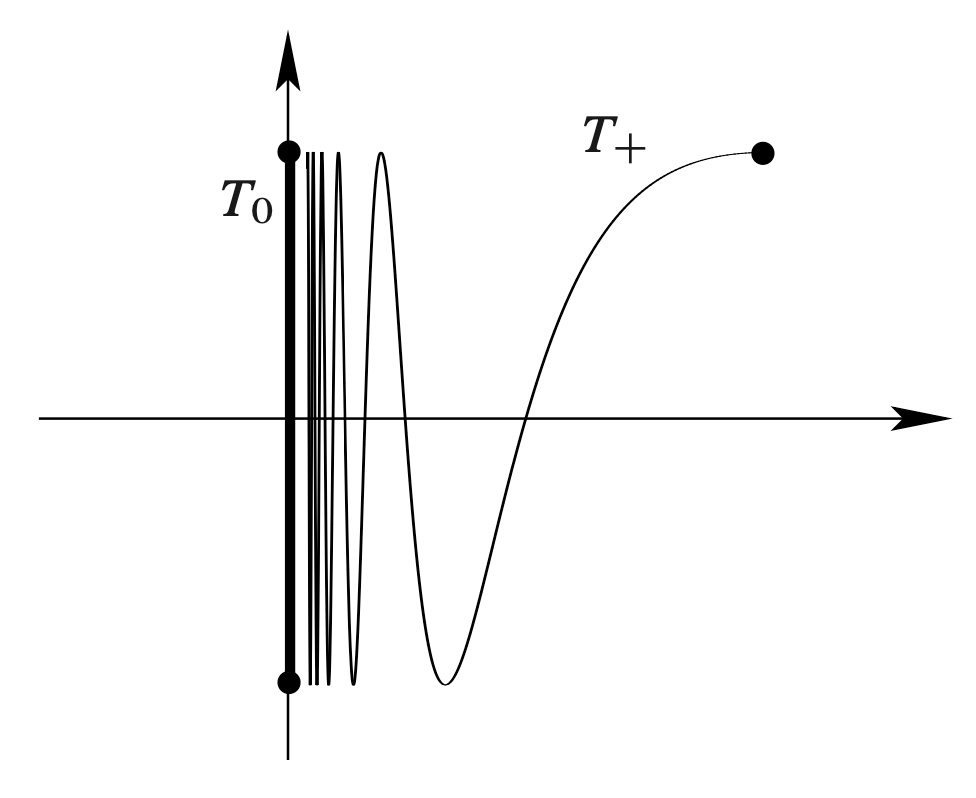
\includegraphics[width=1.3\textwidth]{figs/top_sine.png}
	% \end{center}
	\caption{The topologist's sine curve}
\end{marginfigure}
\begin{definition}
	We say that $X$ is \tb{path-connected} if for every $p,q \in X$, there is a path in $X$ from $p$ to $q$. 
	The book mentions \tb{arc-connected} spaces, which for our purposes can be considered equivalent, but Ref [10] has the subtle details. Path-connectedness is stronger in general than connectedness. Here is a classic example of a space $T$ that is connected but not path-connected. Define subsets of the plane by
	$$
	\begin{aligned}
		T_0 &= \br{(x,y):x=0 \text{ and } y\in[-1,1]}\\
		T_+ &= \br{(x,y):x\in(0,2/\pi] \text{ and } y=\sin (1/x)}
	\end{aligned}
	$$
	The space $T=T_0\cup T_+$ is called the \tb{topologist's sine curve}.
\end{definition}

\marginnote{The \emph{Poincaré conjecture} (now theorem) is that every simply connected compact 3-manifold is homeomorphic to the 3-sphere.}
\begin{definition}
	If $X$ is path-connected and its fundamental group $\pi_1(X)$ is trivial, we say that $X$ is \tb{simply connected}. This means that every loop in $X$ can be continuously shrunk to a single basepoint which is kept fixed. Equivalently any two paths between two points $p, q$ are homotopic. Here is the inclusion of connectivity:
	$$
	\tb{Simply Connected} \subset \tb{Path-Connected} \subset \tb{Connected}
 	$$
\end{definition}

\begin{definition}
	\tb{Closed and Exact Forms:}
	$$
	df\begin{cases}
		=0,\quad&\text{$f$ is closed}\\
		\ne0,&\text{$df$ is exact}\\
	\end{cases}
	$$
\end{definition}


\begin{example}
	Show that this 1-form $E$ is closed\mn{$$E=\frac{xdy-ydx}{x^2+y^2}$$}. Show that $\int_{\gamma_0}E=-\pi$ and $\int_{\gamma_1}E=\pi$.
\end{example}
\sol Saying that $E$ is exact, and therefore also closed by $d^2\phi = 0$ is incorrect because $E$ is not well defined when $r=0$. To really show that $E$ is closed we take the differential of $E$ and find that $dE=0$. I will leave the argument for this in Pg 117 of Ref [2] and the actual calculation of $dE=0$ is in Ref [9].\\\\
We are allowed to use polar coordinates with the paths $\gamma_0, \gamma_1$ that avoid the origin, and the integrals are
$$
\int_{\gamma_0} E = \int_{\pi}^{0} d\phi = -\pi, \quad \int_{\gamma_1} E = \int_{\pi}^{2\pi} d\phi = \pi
$$
% For points outside the origin, we may switch to polar coordinates
% $$
% x = r\cos\phi, \quad y = r\sin\phi
% $$
% so we have for $r \ne 0$
% $$
% \begin{aligned}
% 	E=\frac{xdy-ydx}{x^2+y^2} &= \frac{r\cos\phi(\sin\phi dr+r\cos\phi d\phi) - r\sin\phi(\cos\phi dr-r\sin\phi d\phi)}{r^2(\cos^2\phi + \sin^2\phi)}\\
% 	&= \frac{r\cos\phi\sin\phi dr+r^2\cos^2\phi d\phi - r\sin\phi\cos\phi dr+r^2\sin^2\phi d\phi}{r^2}\\
% 	&= \frac{\cancel{r\cos\phi\sin\phi dr}+\cancel{r^2}(\cos^2\phi+\sin^2\phi) d\phi \cancel{- r\sin\phi\cos\phi dr}}{\cancel{r^2}}\\
% 	&= d\phi
% \end{aligned}
% $$

\begin{definition}
	\tb{Poincaré Lemma:} Let $U \subset \R^n$ be contractible. Let $\omega \in \Omega^{k+1}(U)$ be closed. Then $\omega$ is exact, i.e. there exists an $\alpha \in \Omega^k(U)$ such that $\omega = d\alpha$. But this statement is \emph{false} for a general (non-Euclidean) manifold $M$, i.e., if $M$ has holes in it.
\end{definition}


\begin{example}\label{b1e81}
	Show that $\R^n$ is simply connected by exhibiting an explicit formula for a homotopy between any two paths between arbitrary points $p,q \in \R^n$.
\end{example}
\sol Let $\gamma_0(t), \gamma_1(t)$ be two paths from $p$ to $q$ in $\R^n$. The \emph{straight-line homotopy} is the smooth function $\gamma:[0,1]\times[0,T]\to \R^n$ defined as
$$
\gamma(s,t) = (1-s)\gamma_0(t)+s\gamma_1(t)
$$
and every loop $\gamma(0)=\gamma(T)=p$ can be shrunk to the point $p$ using this homotopy. Thus $\R^n$ is simply connected.


\begin{example}
	Show that a 1-form $E$ is exact if and only if $\int_\gamma E = 0$ for all loops $\gamma$. (Hint: if $\omega$ is not exact, show that there are two smooth paths $\gamma,\gamma^\prime$ from some point $x \in M$ to some point $y \in M$ such that $\int_\gamma \omega\ne\int_{\gamma^\prime} \omega$. Use these paths to form a loop, perhaps only piecewise smooth.)
\end{example}
\sol Let $E=-d\omega$ be an exact 1-form and $\gamma:[0,1]\to M$ a loop based at $p \in M$. Then
$$
\begin{aligned}
	\oint_\gamma E &= -\oint_\gamma d\phi\\
	&= -\int_{0}^{1} d\phi(\gamma^\prime(t)) dt\\
	&= -\int_{0}^{1} \gamma^\prime(t)(\phi) dt\marginnote{Pg 41 of text: $df(v)=v(f)$}\\
	&= -\int_{0}^{1} \frac{d}{dt}\phi(\gamma(t))dt\marginnote{Chain rule in reverse}\\
	&= -\phi(\gamma(1))+\phi(\gamma(0))\\
	&= -\phi(p)+\phi(p)\\
	&= 0
\end{aligned}
$$
Conversely, let $E$ be not exact. On a simply connected manifold, every closed form is exact, so if $dE=0$ then our manifold is not simply connected, implying the existence of non-homotopic smooth paths $\gamma_0, \gamma_1$ from $p$ to $q$ such that
$$
\int_{\gamma_0} E \ne \int_{\gamma_1} E
$$
We can therefore construct a piecewise-smooth loop $\tilde{\gamma}$ that traverses $\gamma_0$ forward and then $\gamma_1$ in reverse with
$$
\oint_{\tilde{\gamma}} E = \int_{\gamma_0} E - \int_{\gamma_1} E \ne 0
$$


\begin{example}\label{b1e83}
	For any manifold $M$, show the manifold $S^1 \cross M$ is not simply connected by finding a 1-form on it that is closed but not exact.
\end{example}
\sol Choosing coordinates $(\theta, x^\mu)$ on $S^1\cross M$, consider the 1-form $\omega=d\theta$. Clearly $d\omega=0$, so the form is closed, and
$$
\oint_\gamma \omega = 2\pi
$$
We have $\oint_\gamma \omega \ne 0$ and therefore $\omega$ is not exact. 
The existence of a 1-form that is closed but not exact $\Rightarrow S^1 \cross M$ is not simply connected.


\begin{example}\label{b1e84}
	Let the $n$-\tb{disk} $D^n$ be defined as\mn{$D^n$ is also called the closed unit ball $\mathbb{\bar{B}}^n$ like in Refs [2, 3]. Also I made the indices contravariant like they should be.}
	$$
	D^n = \br{(x^1, \cdots, x^n): (x^1)^2 + \cdots + (x^n)^2 \le 1}.
	$$
	Show that $D^n$ is an $n$-manifold with boundary in an obvious sort of way.
\end{example}
\sol Consider the map $\pi \circ \sigma^{-1}: \R^n \to \R^n$, where $\sigma:S^n \to \R^n$ is the stereographic projection (Ex \ref{b1e3}) and $\pi$ is a projection from $\R^{n+1}$ to $\R^n$ that omits some coordinate other than $(x_n)$. These maps act as charts $\varphi_\alpha$ that allow us to call $D^n$ an $n$-manifold with boundary. Each point in $S^{n-1}$ is a boundary point, and each point in the open unit ball
$$
\mathbb{B}^n = \br{(x^1, \cdots, x^n): (x^1)^2 + \cdots + (x^n)^2 {\:\color{red}<\:} 1}.
$$
is an interior point.


\begin{example}
	Check that the definition of tangent vectors in Sec \ref{b1c3} really does imply that the tangent space at point on the boundary of an $n$-dimensional manifold with boundary is an $n$-dimensional vector space.
\end{example}
\sol The points on the boundary have their special coordinate $x^n$ mapped to a non-negative real in the chart $\mathbb{H}^n$, even if $x^n$ is negative on the open set of the manifold. The derivative remains smooth, and linearity and Leibniz rule will continue to apply, which allow us to prove the vector space axioms.


\begin{definition}
	If $f$ is any real-valued or vector-valued function on a topological space $M$, the \tb{support} of $f$, denoted by $\supp f$, is the closure of the set of points where $f$ is nonzero:
	$$
		\supp f = \overline{\{p \in M:f(p)\ne 0\}}.
	$$
\end{definition}


\begin{example}
	For the mathematically inclined reader: prove that $\int_M \omega$ is independent of the choice of charts and partition of unity.
\end{example}
\sol \marginnote{Ref [3] Pg 404}For $U, V$ open subsets of $\R^n$ or $\mathbb{H}^n$ we claim that under some diffeomorphism $G:U \to V$ $$\int_V\omega = \pm \int_U G^*\omega$$\underline{First} we show that $\int_M \omega$ is independent of the choice of smooth charts whose domain contains $\supp \omega$.\\\\
Suppose $(U,\varphi)$ and $(\tilde{U},\tilde{\varphi})$ are two smooth charts such that $\supp \omega \subseteq U \cap \tilde{U}$. If both charts are positively oriented or both are negatively oriented, then $\tilde{\varphi} \circ \varphi^{-1}$ is an orientation-preserving diffeomorphism from $\varphi(U \cap \tilde{U})$ to $\tilde{\varphi}(U \cap \tilde{U})$, and we have\mn{Based on our above claim we can define the integral of $\omega$ over $M$ to be$$\int_M\omega = \pm \int_{\varphi(U)} (\varphi^{-1})^* \omega$$where the sign depends on the orientation of the chart $\varphi$.}
$$
\begin{aligned}
	\int_{\tilde{\varphi}(\tilde{U})} (\tilde{\varphi}^{-1})^* \omega &= \int_{\tilde{\varphi}(U \cap \tilde{U})} (\tilde{\varphi}^{-1})^* \omega\\
	&= \int_{\varphi(U \cap \tilde{U})} (\tilde{\varphi} \circ \varphi^{-1})^* (\tilde{\varphi}^{-1})^* \omega\\
	&= \int_{\varphi(U \cap \tilde{U})} (\varphi^{-1})^* (\tilde{\varphi})^* (\tilde{\varphi}^{-1})^* \omega\\
	&= \int_{\varphi(U \cap \tilde{U})} (\varphi^{-1})^* \cancel{(\tilde{\varphi})^* (\tilde{\varphi}^{-1})^*} \omega\\
	&= \int_{\varphi(U)} (\varphi^{-1})^* \omega\\
\end{aligned}
$$
If the charts \begin{marginfigure}
	\begin{center}
		\hspace*{-10px}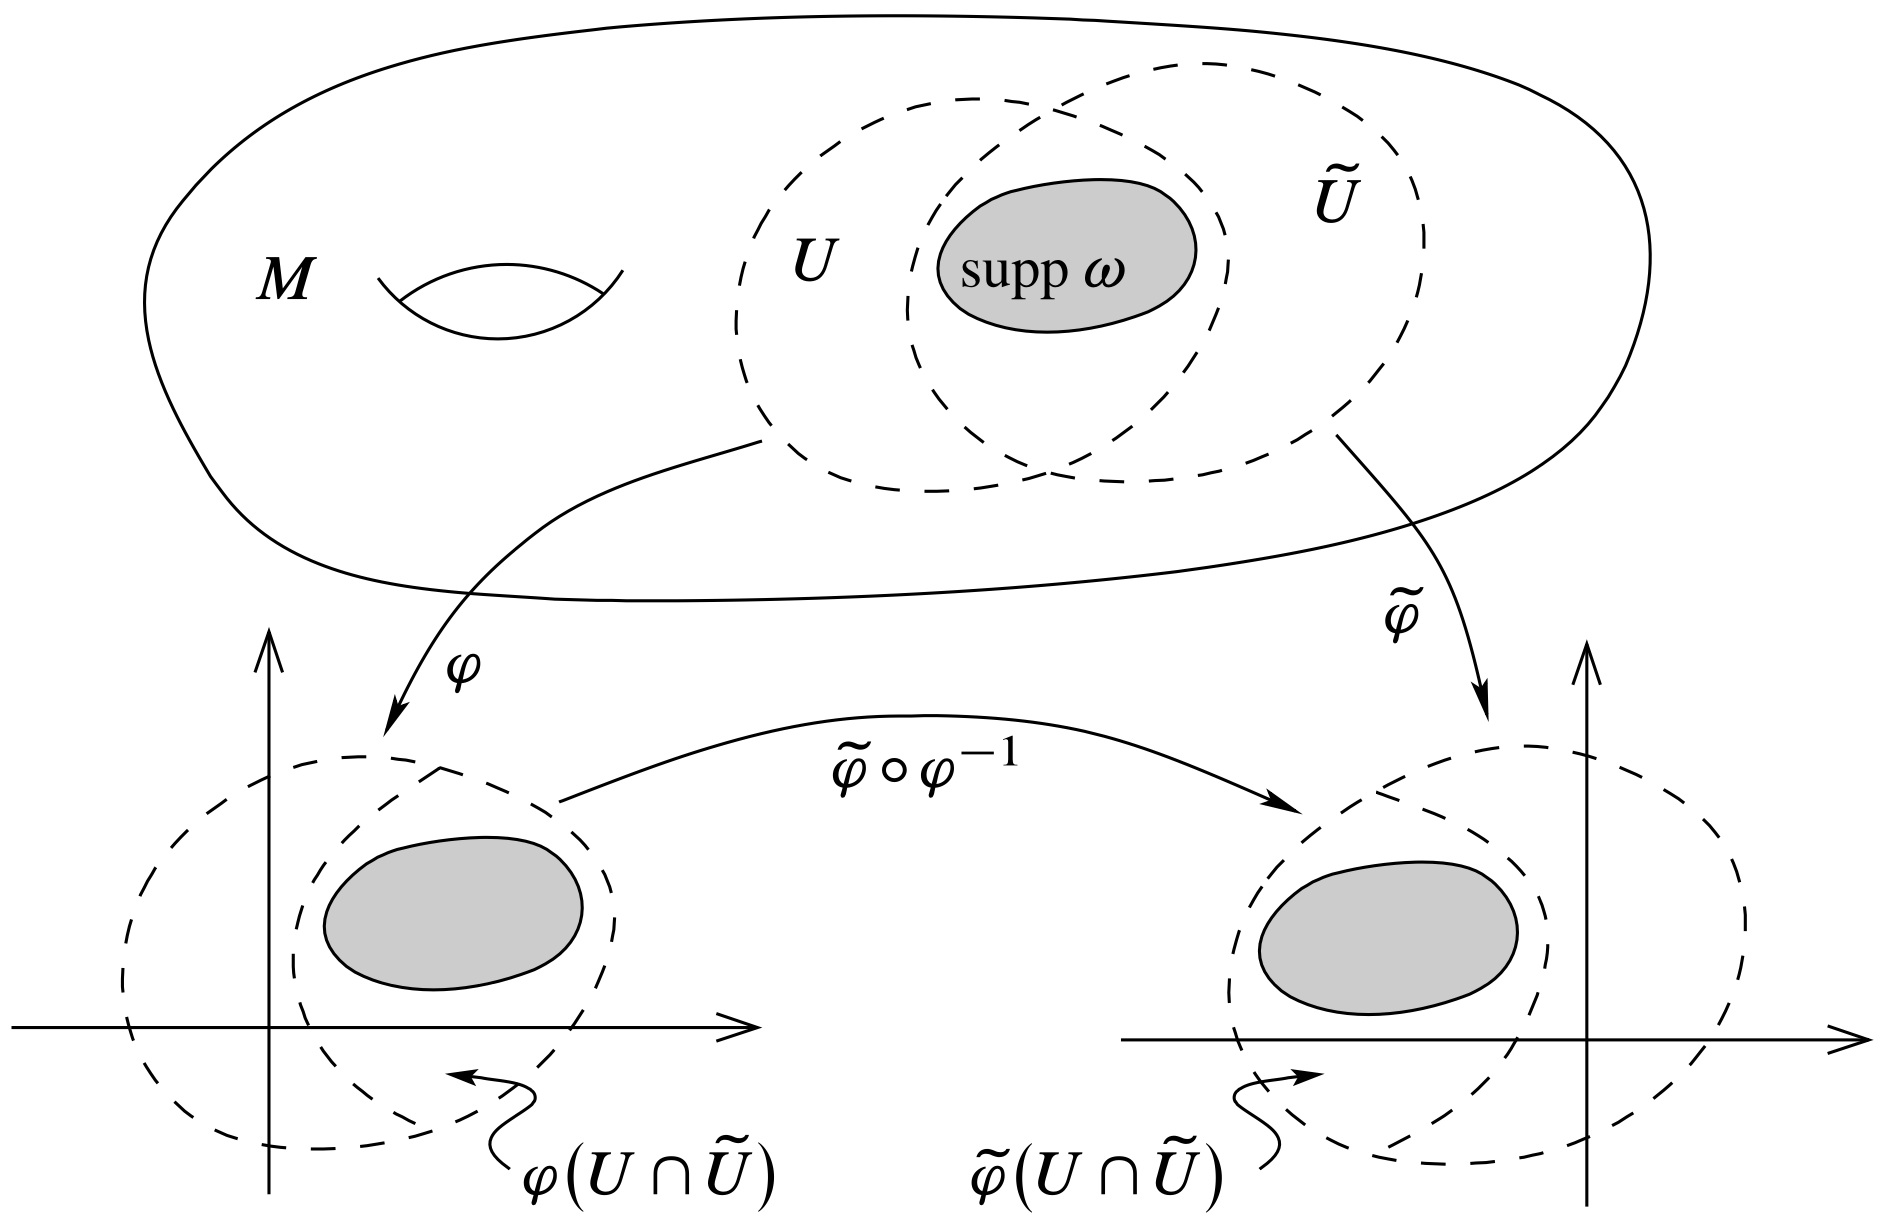
\includegraphics[width=1.5\textwidth]{figs/coord_indep.png}
	\end{center}
	\caption{Coordinate independence of the integral}
\end{marginfigure}
are oppositely oriented, then the two definitions given in the margin note have opposite signs, but this is compensated by the fact that $\tilde{\varphi} \circ \varphi^{-1}$ is orientation-preserving. In either case the two definitions of $\int_M \omega$ agree.\\\\
\underline{Next} we show that $\int_M \omega$ is independent of the partition of unity. Suppose we had two partitions of unity $\sum_\alpha f_\alpha = \sum_\beta g_\beta = 1$. For each $\alpha$ we compute
$$
\int_M f_\alpha \omega = \int_M \p*{\sum_\beta g_\beta} f_\alpha \omega = \sum_\beta \int_M g_\beta f_\alpha \omega
$$
Summing over $\alpha$ we obtain
$$
\sum_\alpha \int_M f_\alpha \omega = \sum_{\alpha, \beta} \int_M g_\beta f_\alpha \omega.
$$
The same argument, starting with $\int_M g_\beta\omega$, shows that
$$
\sum_\beta \int_M g_\beta \omega = \sum_{\alpha, \beta} \int_M g_\beta f_\alpha \omega.
$$
Thus both definitions yield the same value for $\int_M \omega$. 


\begin{example}
	Show that $\partial D^n = S^{n-1}$, where the $n$-disk $D^n$ is defined as in Ex \ref{b1e84}.
\end{example}
\sol From Ex \ref{b1e84}, $\partial D^n = S^{n-1}$ are the precisely the points that get mapped by the charts $\varphi_\alpha$ to the boundary of the closed half-space.


\begin{example}
	Let $M = \br{0,1}$. Show that Stokes' theorem in this case is equivalent to the fundamental theorem of calculus:
	$$
		\int_{0}^{1} f^\prime(x)\:dx = f(1) - f(0).
	$$
\end{example}
\sol By Stokes' theorem
$$
\int_{0}^{1} f^\prime(x)dx = \int_{0}^{1} df = \int_{\partial[0, 1]} f(x) = f(1) +(- f(0)) = f(1) - f(0)
$$
where $\partial[0, 1] = \br{0}^- \cup \br{1}^+$ where the sign denotes orientation. This is because we view the interval as an oriented chain with oriented boundary.\marginnote{Ref [1] Pg 163}


\begin{example}
	Let $M = [0,\infty)$, which is not compact. Show that without the assumption that $f$ vanishes outside a compact set, Stokes' theorem may not apply. (Hint: in this case Stokes' theorem says $\int_{0}^{\infty} f^\prime(x)\:dx = - f(0)$.)
\end{example}
\sol By Stokes' theorem we get the incorrect result
$$
\int_{0}^{\infty} f^\prime(x)dx = \int_{\partial[0, \infty]} f(x) = - f(0)
$$
because $\partial[0, \infty] = \br{0}^-$. But clearly this integral diverges for $f(x)=x\Rightarrow f^\prime(x) = 1$ for example.
\begin{marginfigure}
	\begin{center}
		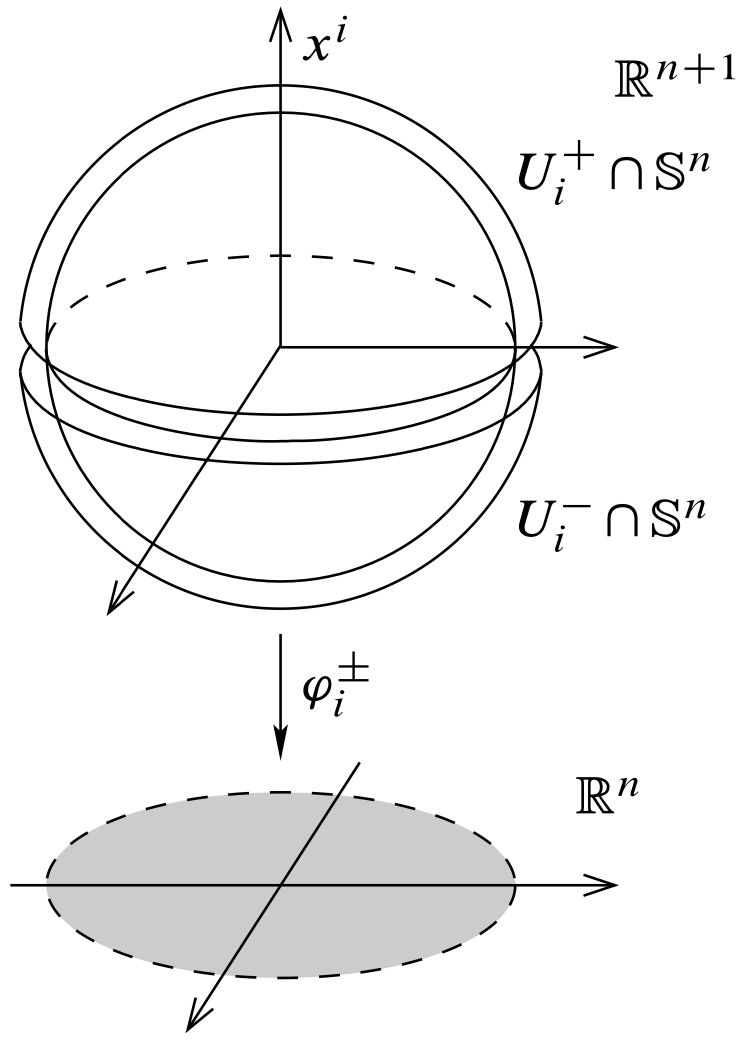
\includegraphics[width=1.2\textwidth]{figs/sn.png}
	\end{center}
	\caption{Charts for $S^n$}
\end{marginfigure} 


\begin{example}\label{b1e90}
	Show that any submanifold is a manifold in its own right in a natural way.
\end{example}
\sol From Ex \ref{b1e4}, imbuing submanifold $S$ with the induced topology guarantees an atlas $\br{(S \cap U_\alpha, \varphi_\alpha|_{S \cap U_\alpha})}$, making $S$ a manifold.


\begin{example}
	Show that $S^{n-1}$ is a compact submanifold of $\R^n$.
\end{example}
\sol The stereographic projections (Ex \ref{b1e3}) take us to a chart that locally looks like an $(n-1)$-dimensional hyperplane in $\R^n$. \marginnote{Ref [3] Pg 5}The two hemispheres form a finite open cover of $S^{n-1}$, this is the ``topological'' way to show compactness. The ``analysis'' way, is that since $S^{n-1} \subset \R^n$
\begin{itemize}
	\item is closed, because it is $\partial D^n$ and boundaries are always closed
	\item bounded, because norm of every point on the sphere equals 1
\end{itemize}by the Heine-Borel theorem $S^{n-1}$ is compact.



\begin{example}
	Show that any open subset of a manifold is a submanifold.
\end{example}
\sol By Ex \ref{b1e90}, where we take $S = \bigcup_\alpha U_\alpha$.


\begin{example}
	Show that if $S$ is a $k$-dimensional submanifold with boundary of $M$, then $S$ is a manifold with boundary in a natural way. Moreover, show that $\partial S$ is a $(k-1)$-dimensional submanifold of $M$.
\end{example}
\sol By Ex \ref{b1e90}, where the charts go to either $\R^n$ or $\mathbb{H}^n$. $\partial S \subset S$ is the set of points that goes to the halfspace.


\begin{example}
	Show that $D^n$ is a submanifold of $\R^n$ in this sense.
\end{example}
\sol $\partial D^n = S^{n-1}$ is the set of points that goes to $\mathbb{H}^n$, while interior points form an open set which is locally Euclidean.


\begin{example}
	Suppose that $S \subset \R^2$ is a 2-dimensional compact orientable submanifold with boundary. Work out what Stokes' theorem says when applied to a 1-form on $S$. This is sometimes called Green's theorem.
\end{example}
\sol Green's theorem in multivariable calculus is:
\begin{marginfigure}
	\begin{center}
		% \vspace*{30px}\hspace*{-65px}
		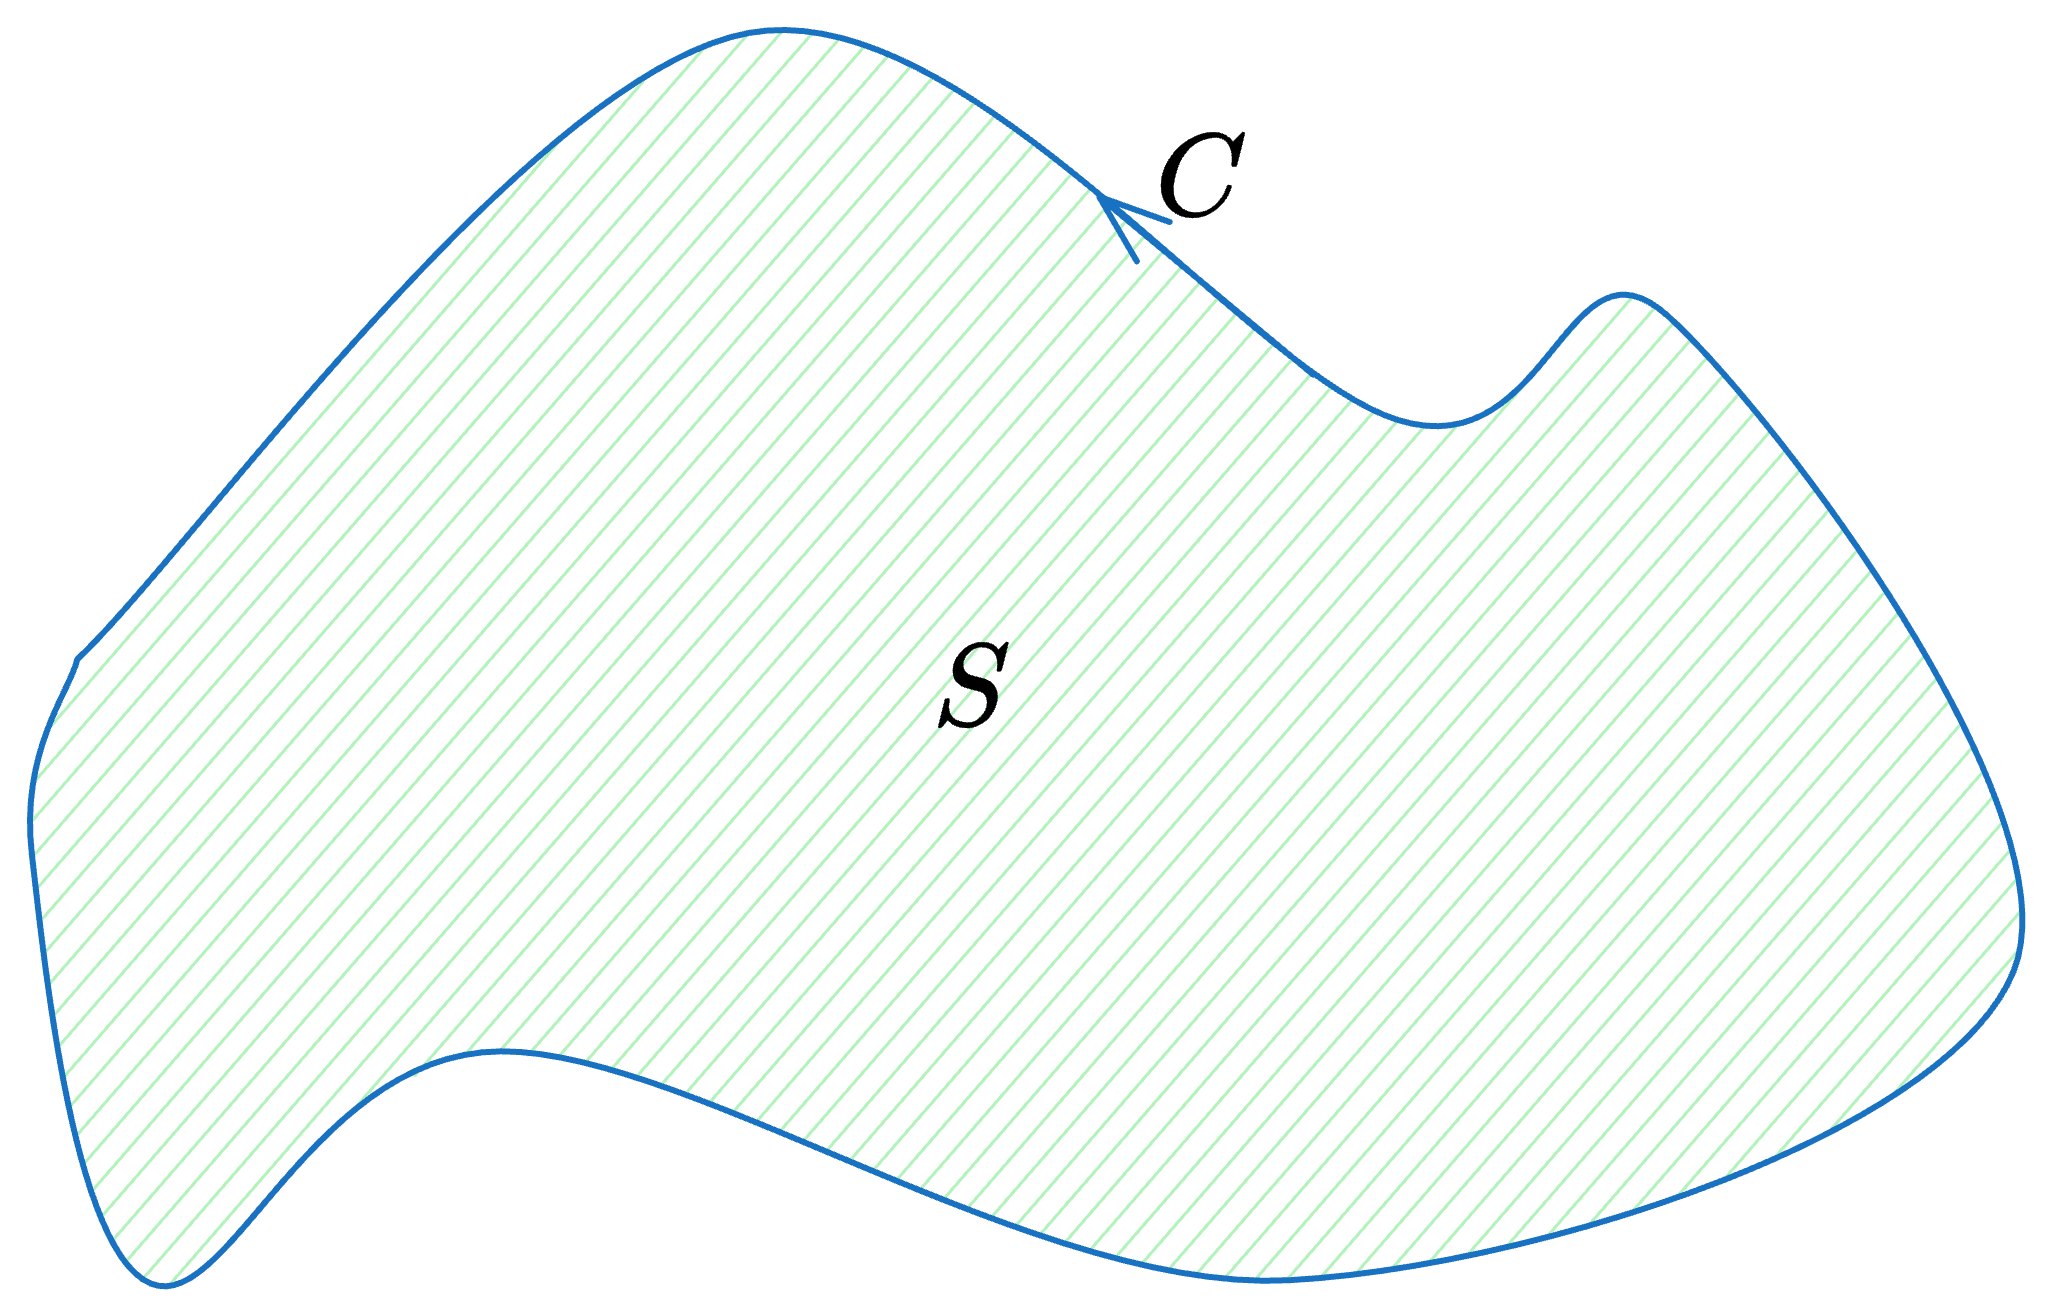
\includegraphics[width=1.2\textwidth]{figs/green.png}
	\end{center}
	\caption{Green's theorem}
\end{marginfigure}
$$
\int_C fdx+gdy = \int_S\p*{\pd{g}{x}-\pd{f}{y}}dxdy
$$
where 
\begin{itemize}
	\item $f,g \in C^\infty(S)$ are some 0-forms or functions defined on the domain $S$
	\item $C = \partial S$ is a counterclockwise oriented contour that is the boundary of $S$
\end{itemize}
Define the 1-form 
$$
\begin{aligned}
	\omega &= fdx+gdy\\
	\Rightarrow d\omega &= d(fdx)+d(gdy)\\
	&= \pd{f}{x}\cancel{dx\wedge dx} + \pd{f}{y}dy\wedge dx + \pd{g}{x}dx\wedge dy + \pd{g}{y}\cancel{dy\wedge dy}\\
	&= \pd{f}{y}dy\wedge dx + \pd{g}{x}dx\wedge dy\\
	&= \p*{\pd{g}{x}-\pd{f}{y}}dx \wedge dy
\end{aligned}
$$ 
which implies Stokes' theorem
$$
	\int_{\partial S} \omega = \int_{S} d\omega
$$

\begin{definition}
	Given a vector field $v$ we can define a linear map taking $k$-forms to $k-1$-forms, called the \tb{interior product}\mn{Also called the \tb{hook product} or \tb{contraction}. Alternative notation is $v\lrcorner\:\omega$.} $\iota_v:\Omega^k(M)\to\Omega^{k-1}(M)$ which satisfies the following properties:
	\begin{itemize}
		\item $\iota_v f = 0$
		\item $\iota_v \omega = \omega(v) := \ip{\omega}{v}$ 
		\item $\iota_v (\mu\wedge\nu) = \iota_v \mu\wedge\nu + (-1)^{\deg \mu} \mu\wedge\iota_v\nu$ 
	\end{itemize}
	where $f$ is a 0-form, $\omega$ is a 1-form, $\mu,\nu$ are forms with arbitrary degree. If $\omega$ is a $k$-form
	$$
	\begin{aligned}
		\omega(v_1,v_2\cdots,v_k) &:= (\iota_{v_1}\omega)(v_2\cdots,v_k)
		&= \iota_{v_k}\iota_{v_{k-1}}\cdots\iota_{v_1}\omega
	\end{aligned}
	$$
	The interior product contracts the volume form along the given vector field, reducing the degree of the differential form by 1.
	% \\\\
	% However the pullback of the map, has a useful property on a Riemannian manifold $(M,g)$. Every submanifold $S\subseteq M$ has an \tb{induced metric} defined as
	% $$
	% (\iota_S^* g)(v,w) = g(v,w)\marginnote{$v,w \in T_pS$}
	% $$
	% which is just the restriction of $g$ to pairs of vectors tangent to $S$.
\end{definition}


\begin{example}
	Suppose that $S \subset \R^3$ is a 2-dimensional compact orientable submanifold with boundary. Show Stokes' theorem applied to $S$ boils down to the classic Stokes' theorem.
\end{example}
\sol Stokes' theorem in multivariable calculus is:
\begin{marginfigure}
	\begin{center}
		\vspace*{35px}\hspace*{-32px}
		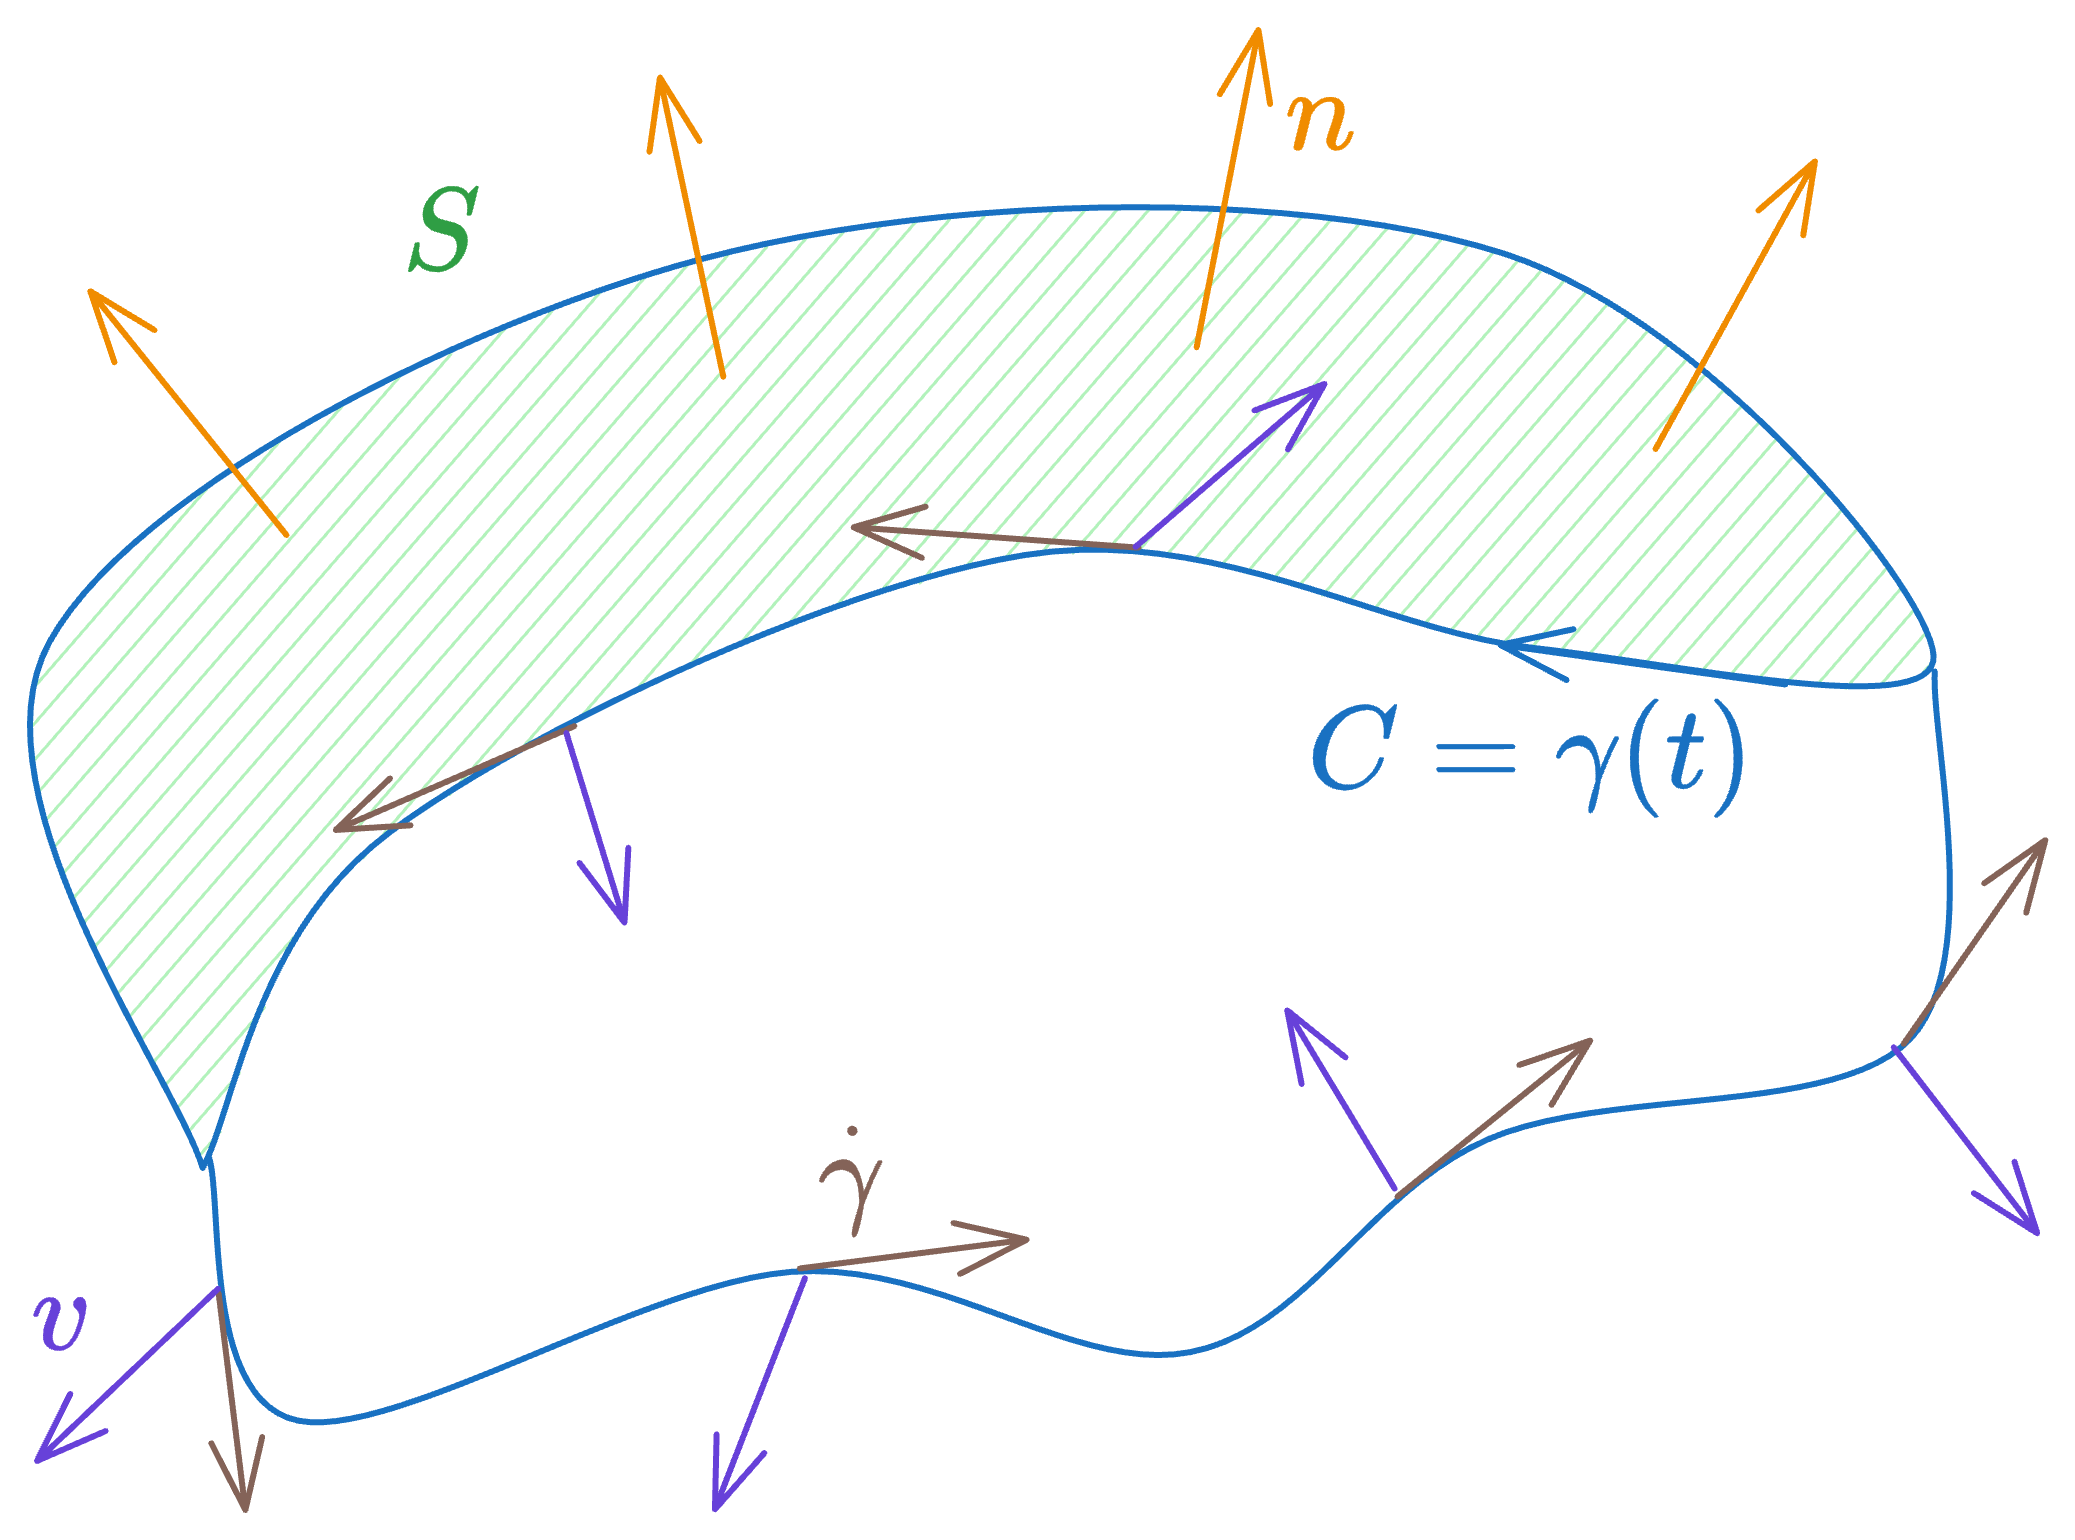
\includegraphics[width=1.5\textwidth]{figs/stokes.png}
	\end{center}
	\caption{Classic Stokes' theorem}
\end{marginfigure}
$$
\int_C \ip{v}{\dot\gamma}dt = \int_S\ip{{\rm curl }\:v}{n}dA
$$
where 
\begin{itemize}
	\item $S$ is a surface with outward normal $n$ and area form $dA$.
	%  The area form $dA$ is defined with respect to the induced metric $\iota_S^* g$ as
	% $$
	% 	dA = \iota_S^*(\iota_n \vol)
	% $$
	\item $C = \partial S$ is the boundary of $S$, which is parametrized by the curve $\gamma:[0,1]\to C$ with tangent $\dot\gamma$
	\item $v$ is a vector field defined everywhere on $\R^3$
\end{itemize}
We define $v^\flat$, the dual of $v$\marginnote{See musical isomorphisms in Ref [24]}, \emph{either} by its action on another vector field $u$, \emph{or} by the interior product
$$
	v^\flat(u) = (v^idx^i)(u^j\partial_j) = v^iu^i = \ip{v}{u} = \iota_u v
$$
The curl is defined in terms of the interior product as
$$
	\iota_{{\rm curl }\:v}\vol = d(v^\flat)\marginnote{See Ref [3], Pg 426}
$$
We note that
$$
\begin{aligned}
	\int_C v^\flat &= \int_{0}^{1} \gamma^*(v^\flat)dt\marginnote{Pulling back 1-form $v^\flat$}\\
	&= \int_{0}^{1} v^\flat(\dot{\gamma}(t))dt\\
	&= \int_C \ip{v}{\dot\gamma}dt
\end{aligned} 
$$
but using Stokes' theorem gives
$$
\begin{aligned}
	\int_C v^\flat &= \int_S d(v^\flat)\\
	&= \int_S\iota_{{\rm curl }\:v}\ub{\vol}{dA \wedge n}\marginnote{See Ref [3], Pg 423, Lemma 16.30 and Pg 426. We need machinery of the induced metric to properly show this. In particular $dA = \iota_S^*(\iota_n \vol)$}\\
	&= \int_S\iota_{{\rm curl }\:v}dA \wedge n + (-1)^2dA \wedge \iota_{{\rm curl }\:v}n\\
	&= \cancel{\int_S\iota_{{\rm curl }\:v}dA \wedge n} + \int_S\ip{{\rm curl }\:v}{n}dA\\
	&= \int_S\ip{{\rm curl }\:v}{n}dA
\end{aligned}
$$
which implies the higher dimensional Stokes' theorem, in the language of differential forms
$$
	\int_{\partial S} \omega = \int_{S} d\omega\marginnote{$\omega=v^\flat$}
$$


\begin{example}
	Suppose that $S \subset \R^3$ is a 2-dimensional compact orientable submanifold with boundary. Show Stokes' theorem applied to $S$ is equivalent to Gauss' theorem, also known as divergence theorem.
\end{example}
\sol Divergence theorem in multivariable calculus is:
\begin{marginfigure}
	\begin{center}
		% \vspace*{35px}\hspace*{-32px}
		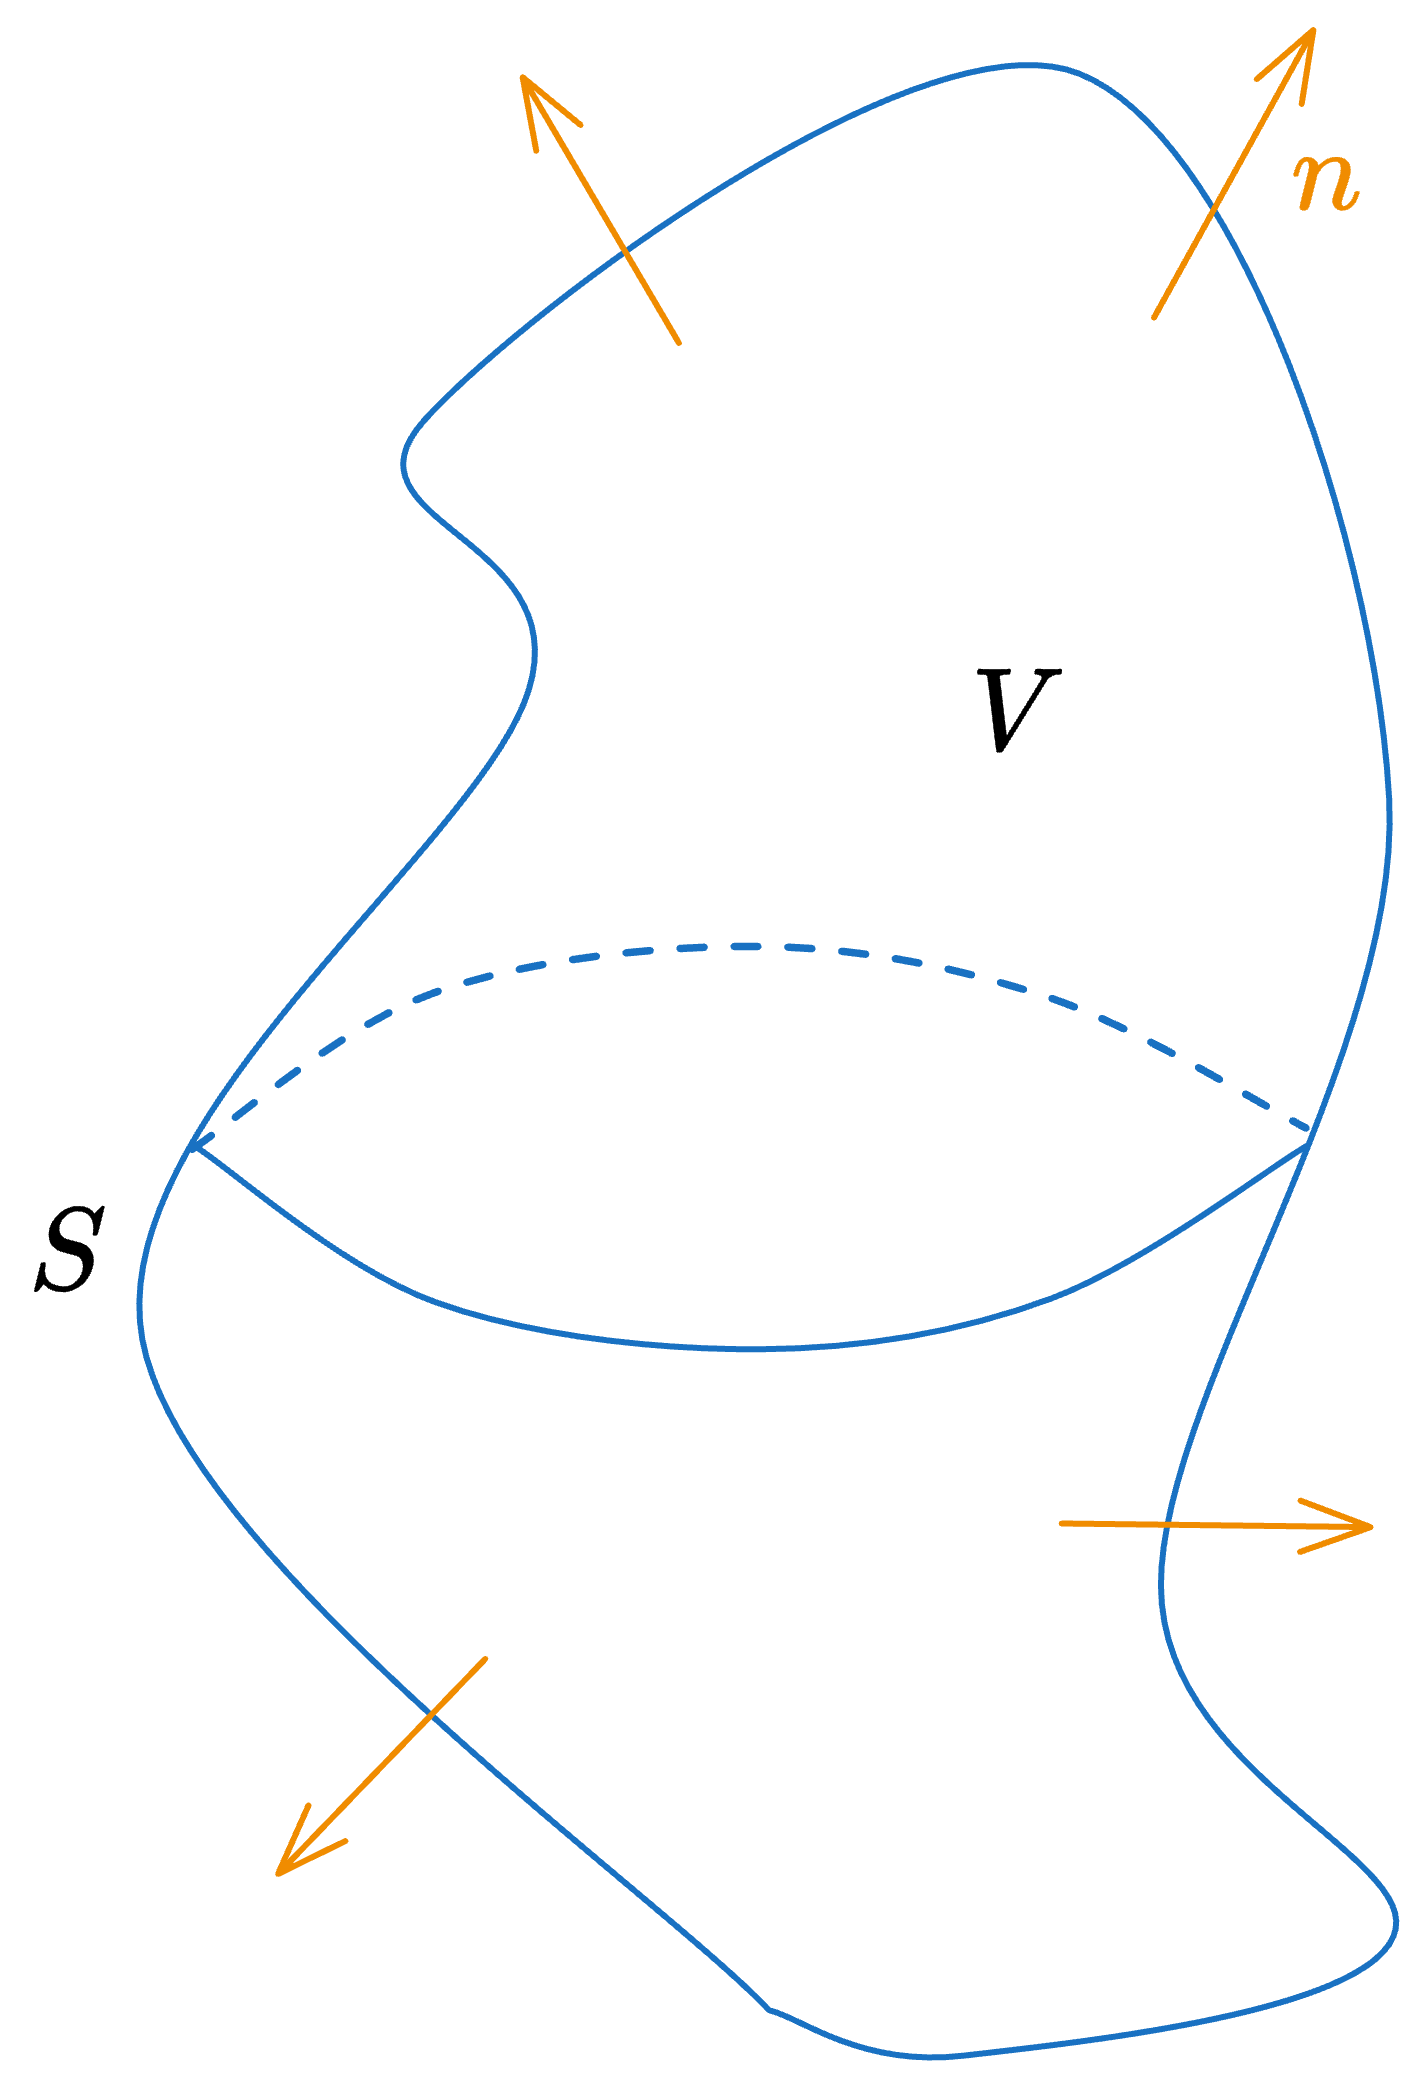
\includegraphics[width=\textwidth]{figs/div.png}
	\end{center}
	\caption{Divergence theorem}
\end{marginfigure}
$$
	\int_S\ip{v}{n}dA = \int_V\ip{{\rm div }\:v}{dV}
$$
First we show
$$
\begin{aligned}
	d(\iota_v dV) &= d(v^1\partial_1 + v^2\partial_2 + v^3\partial_3) \lrcorner\: dx^1+dx^2+dx^3\\
	&= d(v^1\partial_1 + v^2\partial_2 + v^3\partial_3) \lrcorner\: dx^1+dx^2+dx^3\\
	&= \ip{{\rm div }\:v}{dV}
\end{aligned}
$$
What follows is
$$
\begin{aligned}
	\int_S\ip{v}{n}dA &= \int_S\iota_v dV\\
	&= \int_Vd(\iota_v dV)\\
	&= \int_V\ip{{\rm div }\:v}{dV}
\end{aligned}
$$
which implies Stokes' theorem
$$
	\int_{\partial S} \omega = \int_{S} d\omega\marginnote{$\omega = \iota_v dV$}
$$


\begin{definition}
	\tb{Poincaré Lemma (redux):} If $U$ is a star-shaped\mn{A subset $U \subseteq \R^n$ is said to be \tb{star-shaped} if there is a point $c \in U$ such that for every $x \in U$, the line segment from $c$ to $x$ is entirely contained in $U$.} open subset of $\R^n$ or $\Hs^n$ then $H^p(U)= \br{0}$ for $p \ge 1$.
\end{definition}


\begin{example}\label{b1e98}
	Show that the pullback of a closed form is closed and the pullback of an exact form is exact.
\end{example}
\sol If $\omega$ is closed, then $d(\phi^*\omega) = \phi^*(d\omega) = 0$, so $\phi^*\omega$ is also closed. If $\omega = df$ is exact, then $\phi^*\omega = \phi^*(df) = d(\phi^*f)$, which is also exact.\marginnote{Ref [3] Pg 442}\\\\
This is because for any smooth map $\phi:M\to N$ between smooth manifolds with or without boundary, the pullback $\phi^*:\Omega^p(N) \to \Omega^p(M)$ carries $Z^p(N)$ into $Z^p(M)$ and $B^p(N)$ into $B^p(M)$.


\begin{example}\label{b1e99}
	Show that given any map $\phi:M\to M^\prime$ there is a linear map from $H^p(M^\prime)$ to $H^p(M)$ given by
	$$
		[\omega] \mapsto [\phi^*\omega]
	$$
	where $\omega$ is any closed $p$-form on $M^\prime$. Call this linear map
	$$
	\phi^*:H^p(M^\prime) \to H^p(M).
	$$
	Show that if $\psi: M^\prime \to M^{\prime\prime}$ is another map, then
	$$
	(\psi\phi)^* = \phi^*\psi^*.
	$$
\end{example}
\sol For a closed $p$-form $\omega$ let
$$
	\phi^*[\omega] = [\phi^*\omega]
$$
If $\omega$ and $\omega^\prime$ are cohomologous, i.e, $\omega^\prime = \omega + d\eta \Rightarrow [\phi^*\omega^\prime] = [\phi^*\omega + d(\phi^*\eta)] = [\phi^*\omega]$, so the map $\phi^*$ is well defined and so is $(\psi\phi)^*:H^p(M^{\prime\prime}) \to H^p(M^\prime) \to H^p(M)$ which is equal to $\phi^*\psi^*$ by Ex \ref{b1e31}.


\begin{example}\label{b1e100}
	Do this. (Hint: Show that $\star dz = rdr \wedge d\theta$.)
\end{example}
\sol Recall that cylindrical coordinates are
$$
dx = \cos\theta dr - r\sin\theta d\theta,\\
dy = \sin\theta dr + r\cos\theta d\theta.
$$
Taking the Hodge dual of $dz$
$$
\begin{aligned}
	\star dz &= dx \wedge dy\\
	&= (\cos\theta dr - r\sin\theta d\theta) \wedge (\sin\theta dr + r\cos\theta d\theta)\\
	&= r\cos^2\theta dr \wedge d\theta - r\sin^2\theta d\theta \wedge dr\marginnote{Cross terms vanish}\\
	&= r\cos^2\theta dr \wedge d\theta + r\sin^2\theta dr \wedge d\theta\\
	&= rdr \wedge d\theta\\
	\Rightarrow \star j &= f(r)\star dz = f(r)r dr \wedge d\theta
\end{aligned}
$$


\begin{example}
	Show that $d\theta = \frac1r dz \wedge dr$.
\end{example}
\sol Taking the Hodge dual of $d\theta$
$$
\begin{aligned}
	\star d\theta &= \star\p*{\frac{xdy-ydx}{x^2+y^2}}\\
	&= \frac{r\cos\theta dz\wedge (\cos\theta dr - r\sin\theta d\theta)- r\sin\theta (\sin\theta dr + r\cos\theta d\theta)\wedge dz}{r^2}\marginnote{Substitute polar coordinates}\\
	&= \frac{r(\cos^2\theta +\sin^2\theta) dz \wedge dr \cancel{- r^2\sin\theta\cos\theta dz\wedge d\theta} + \cancel{r^2\sin\theta\cos\theta dz\wedge d\theta}}{r^2}\\
	&= \frac1r dz \wedge dr
\end{aligned}
$$


\begin{example}
	Check that $d\star B = \star j$ holds if and only if $g^\prime(r) = rf(r)$.
\end{example}
\sol Taking the exterior derivative of $\star B$
$$
\begin{aligned}
	d\star B &= dg(r)d\theta\\
	\star j &= g^\prime(r)(dr \wedge d\theta)\marginnote{If $d\star B = \star j$}\\
	f(r)r(dr \wedge d\theta) &= g^\prime(r)(dr \wedge d\theta)\marginnote{Result from Ex \ref{b1e100}}\\
	\Rightarrow f(r)r &= g^\prime(r)
\end{aligned}
$$


\begin{example}
	Work out all the details. (Hint - define maps $p_i:T^n \to S^1$ corresponding to projection down to the $i$-th coordinate, where $1 \le i \le n$, and let $d\theta_i = p_i^*d\theta$.)
\end{example}
\sol The projection map looks like
$$
\begin{aligned}
	p_i:&\ub{S^1 \cross S^1\cross \cdots \cross S^1}{n\text{ times}} \to S^1\\
	&:(\theta_1, \cdots, \theta_i, \cdots, \theta_n) \mapsto \theta_i
\end{aligned}
$$
By Ex \ref{b1e98} we know that $d\theta_i$ is closed because pullback of a closed form is closed. By Ex \ref{b1e83}, if we take $M$ to be $S^{n-1}$ we have $d\theta$ is not exact because
$$
\oint_{S^1} d\theta = 2\pi \ne 0
$$
Alternatively, by Ex \ref{b1e99} the pullback of $d\theta$ is a linear map from $H^p(S^1)$ to $H^p(T^n)$ that is in the same cohomology class as $d\theta$, i.e, closed but not exact.


\begin{example}\label{b1e104}
	In the space $\R \cross S^2$ with the metric $g$ given above, let $E$ be the 1-form
	$$
		E = e(r)dr.
	$$
	Show that $dE=0$ holds no matter what the function $e(r)$ is, and show that $d\star E=0$ holds when
	$$
		e(r)=\frac{q}{4\pi f(r)^2}.
	$$
\end{example}
\sol Calculating $dE$
$$
dE = d(e(r)dr) = \partial_r(e(r)) dr \wedge dr = 0
$$
which means $E$ is closed independent of the choice of $e(r)$.\\\\
Given the metric $g_{\mu\nu}$ on Pg 144, the volume form is
$$
\begin{aligned}
	\vol &= \sqrt{|\det (g)|} dr \wedge d\phi \wedge d\theta\\
	&= \sqrt{f(r)^4 \sin^2\phi} dr \wedge d\phi \wedge d\theta\\
	&= \ub{f(r)^2 \sin\phi}{} dr \wedge \ub{d\phi \wedge d\theta}{}\\
	&= dr \wedge \star dr
\end{aligned}
$$
where the bracket terms constitute $\star dr$. Calculating $d\star E$:
$$
\begin{aligned}
	d\star E &= d(e(r) \star dr)\\
	&= d(e(r) f(r)^2 \sin\phi\:d\phi \wedge d\theta)\\
	&= \partial_r(e(r) f(r)^2) \sin\phi\:dr \wedge d\phi \wedge d\theta
\end{aligned}
$$
Setting this to zero implies\marginnote{The constant may have something to do with Coulomb's law which gives electric field for a spherically symmetric charge of radius $r$:
$$\tb{E}(\tb{r}) = \frac{q}{4\pi\varepsilon_0}\frac{\hat{\tb{r}}}{r^2}$$}
$$
\begin{aligned}
	\partial_r(e(r) f(r)^2) &= 0\\
	\Rightarrow e(r) f(r)^2 &= \frac{q}{4\pi}\\
	\Rightarrow e(r) &= \frac{q}{4\pi f(r)^2}
\end{aligned}
$$
for some chosen constant $\frac{q}{4\pi}$.


\begin{example}
	Find a function $\phi$ with $E=d\phi$.
\end{example}
\sol $E$ remains exact for some loop $\gamma$ with some $r \in \R$ fixed. The scalar potential is
$$
\phi(r) = -\int_\gamma E = -\frac{q}{4\pi} \int_\gamma \frac{1}{f(x)^2} dx
$$


\begin{example}
	Let $S^2$ denote any of the 2-spheres of the form $\br{r} \cross S^2 \subset \R \cross S^2$, equipped with the above volume form. Show that
	$$
		\int_{S^2} \star E = q.
	$$
\end{example}
\sol Integrating the Hodge dual of $E$
$$
\begin{aligned}
	\int_{S^2} \star E &= \int_{S^2} e(r) f(r)^2 \sin\theta\:d\theta \wedge d\phi\marginnote{From Ex \ref{b1e104}, except we relabel $\phi \leftrightarrow \theta$ for some reason}\\
	&= e(r) f(r)^2 \int_{S^2} \sin\theta\:d\theta \wedge d\phi\marginnote{We take $r$ is constant in this space}\\
	&= \frac{e(r) f(r)^2}{r^2} \int_{S^2} \ub{r^2\sin\theta\:d\theta \wedge d\phi}{\vol}\\
	&= \frac{e(r) f(r)^2}{r^2} \int_{S^2} \vol\\
	&= \frac{e(r) f(r)^2}{r^2} 4\pi r^2\marginnote{Area of the sphere is a 2-dimensional volume}\\
	&= 4\pi e(r) f(r)^2\\
	&= q
\end{aligned}
$$


\begin{example}
	With this clue, work out a careful answer to the riddle\mn{What integral gives the answer $-q$?}.
\end{example}
\sol Choosing the volume form $\vol = \pm r^2\sin\theta\:d\theta \wedge d\phi$ gives us charge $\pm q$.


\begin{example}
	Describe how this result generalizes to spaces of other dimensions.
\end{example}
\sol In $n$ dimensions a space must have non-zero $H^{n-1}(\R \cross S^{n-1})$ in order for there to be a surface $S^{n-1}$ with $\int_{S^{n-1}} E \ne 0$ when $\rho = 0$.


\begin{example}
	Show using Cartesian coordinates with $\omega$ is closed on $\R^3 - \br{0}$.
\end{example}
\sol Taking the first term of $d\omega = d\omega_x + d\omega_y + d\omega_z$
$$
\begin{aligned}
	d\omega_x &= d\p*{\frac{x\:dy\wedge dz}{(x^2+y^2+z^2)^{3/2}}}\\
	&= \partial_x\p*{\frac{x}{(x^2+y^2+z^2)^{3/2}}}dx\wedge dy\wedge dz\\
	&= \p*{\frac{-2 x^2+y^2+z^2}{\left(x^2+y^2+z^2\right)^{5/2}}}dx\wedge dy\wedge dz\\
\end{aligned}
$$
The terms cancel out
$$
d\omega = \p*{\frac{-2x^2-2y^2-2z^2+2 (x^2+y^2+z^2)}{\left(x^2+y^2+z^2\right)^{5/2}}}dx\wedge dy\wedge dz = 0
$$


\begin{example}
	Generalize these examples and find an $(n-1)$-form on $\R^n - \br{0}$ that is closed but not exact. Conclude that $H^{n-1}(\R^n - \br{0})$ is non-zero.
\end{example}
\sol Generalizing
$$
\omega = \frac{x^1\: dx^2 \wedge \cdots \wedge dx^n + x^2\: dx^3 \wedge \cdots \wedge dx^n \wedge dx^1 + \cdots + x^n\: dx^1 \wedge \cdots \wedge dx^{n-1}}{\p{(x^1)^2+\cdots+(x^n)^2}^{n/2}}
$$
and $H^{n-1}(\R^n - \br{0})$ is 1-dimensional, containing a single $(n-1)$-dimensional hole.


\begin{example}
	Check this. (Hint: show that $B = (m/4\pi)\sin\phi\:d\phi \wedge d\theta$.\mn{Again, my ordering is different from the book})
\end{example}
\sol From Ex \ref{b1e104}
$$
B = \frac{m}{4\pi f(r)^2}\star dr = \frac{m}{4\pi \cancel{f(r)^2}} \cancel{f(r)^2} \sin\phi\:d\phi \wedge d\theta = \frac{m}{4\pi} \sin\phi\:d\phi \wedge d\theta
$$
So the integral becomes
$$
\int_{S^2} B = \frac{m}{4\pi} \int_{0}^{\pi} \sin\phi\:d\phi \int_{0}^{2\pi} d\theta = \frac{m}{\cancel{4\pi}} \cancel{2 \cdot 2\pi} = m
$$





% ----------------------------------------------------------------------
%           Book 2
% ----------------------------------------------------------------------
\newpage
\part{Gauge Fields}






\section{Symmetry}\label{b2c1}




\begin{example}\label{b2e1}
	Show that $\SO(3,1)$ contains the Lorentz transform mixing up the $t$ and $x$ coordinates\mn{We call these $x^0$ and $x^1$ in this problem for spacetime vector $x$}:
	$$
	\begin{pmatrix}
		\cosh\phi&-\sinh\phi&0&0\\
		-\sinh\phi&\cosh\phi&0&0\\
		0&0&1&0\\
		0&0&0&1
	\end{pmatrix}
	$$
\end{example}
\sol Call this matrix $\Lambda$, and let it act on some spacetime vector $x$
$$
T_\mu^\nu x^\mu = \begin{pmatrix}
	\cosh\phi x^0 -\sinh\phi x^1\\
	-\sinh\phi x^0 \cosh\phi x^1\\
	x^2\\
	x^3
\end{pmatrix}
$$
which mixes up $x^0, x^1$ components. Now take two transformed vectors $v$ and $w$ and act them with the $(3,1)$ metric
$$
\begin{aligned}
	g(Tv, Tw) &= -(\cosh\phi v^0 -\sinh\phi v^1)(\cosh\phi w^0 -\sinh\phi w^1)\\
	&+ (-\sinh\phi v^0 +\cosh\phi v^1)(-\sinh\phi w^0 +\cosh\phi w^1)\\
	&+ v^2w^2 + v^3w^3\\
	&= -v^0w^0 + v^1w^1+v^2w^2 + v^3w^3\\
	&= g(v,w)
\end{aligned}
$$
Moreover, $\det (T) = \cosh^2\phi -\sinh^2\phi = 1$ so $T$ is orthonormal. Therefore $T \in \SO(3,1)$ and analogously for the other transforms that mix up $x^0, x^2$ and $x^0, x^3$.


\begin{example}
	Show that $\SO(3,1)$ contains neither parity,
	$$
	P:(t,x,y,z)\mapsto(t,-x,-y,-z),
	$$
	nor time-reversal
	$$
	T:(t,x,y,z)\mapsto(-t,x,y,z),
	$$
	but that these lie in O$(3,1)$. Show that the product $PT$ lies in SO$(3, 1)$.
\end{example}
\sol $P$ and $T$ preserve the metric, but not the determinant: $\det (P) = \det (T) = -1$, so they are not in $\SO(3,1)$. However
$$
\det (PT) = \det (P) \det (T) = 1
$$
so $PT \in \SO(3,1)$.

\begin{definition}
	\tb{Poincaré group} deals with the kinematics of particles - their motion and transformations through spacetime. \tb{Charge conjugation} deals with the internal properties of particles, not their motion.\\\\
	Together they describe the \tb{CPT symmetry} in quantum field theory. Ref [18] has more.
\end{definition}

\begin{example}
	Show that SL$(n, \R)$, SL$(n,\C)$, O$(p,q)$, SO$(p,q)$, U$(n)$ and SU$(n)$ are really matrix groups, that is, that they are closed under matrix multiplication, inverses, and contain the identity matrix.
\end{example}
\sol We need to show closure, inverse and identity:
\begin{itemize}
	\item Let $u,v$ be vectors in $\C^n$ with some metric $g$ and $A, B$ be matrices in some group $G$. For $G$ one of O$(p,q)$, U$(n)$
	$$
	\begin{aligned}
		\ip{(AB)v}{(AB)w} &= \ip{A(Bv)}{A(Bw)}\\
		&= \ip{Bv}{Bw}\\ 
		&= \ip{v}{w}
	\end{aligned}
	$$
	because both O$(p,q)$, U$(n)$ preserve the usual inner product on $\C^n$. We see that $AB \in G$, implying $G$ is closed nuder multiplication. The same holds for SL$(n, \R)$, SL$(n,\C)$, SO$(p,q)$ and SU$(n)$ with the additional requirement that $\det (A) = \det (B) = \det (AB) = 1$.
	
	\item If $G$ is O$(p,q)$, the inverse element of $A \in G$ is $A^\intercal$. If $G$ is U$(n)$, the inverse element of $A \in G$ is $A^\dag$. For SL$(n, \R)$, SL$(n,\C)$, SO$(p,q)$ and SU$(n)$, we are guaranteed that $A \in G$ is invertible.
	
	\item $\id$ is the identity element for all $G$.
\end{itemize}


\begin{example}
	Show that the groups GL$(n, \R)$, GL$(n,\C)$, SL$(n, \R)$, SL$(n,\C)$, O$(p,q)$, SO$(p,q)$, U$(n)$ and SU$(n)$ are Lie groups. (Hint: the hardest part is to show that they are submanifolds of the space of matrices.)
\end{example}
\sol Let $A,B$ be matrices in GL$(n, \C)$.\marginnote{See also Ref [3] Pg 144} The product map acts elementwise as $(ab)_{ij} = a_{ik}b_{kj}$, which is smooth since the product is a polynomial of the elements. Inversion by Cramer's rule
$$
A \mapsto A^{-1} = \frac{A^\dag}{\det (A)}
$$
is also smooth since adjoint $A^\dag$ are polynomials of entries of $A$.\\\\
Let $M(n,\C)$ be the space of $n \times n$ matrices over $\C$. This is trivially a smooth $2n^2$-manifold since it is homeomorphic to $\R^{2n^2}$. The map $\det:M(n,\C)\to \C$ is smooth, so GL$(n,\C) = \det^{-1}(\C \setminus \br{0})$ is an open subset of $M(n,\C)$ and therefore a submanifold by Ex \ref{b1e90}, so GL$(n,\C)$ and thus GL$(n,\R)$ are Lie groups.\\\\
Closed subgroups of Lie groups are Lie groups, so the rest are all Lie groups.


\begin{example}
	Given a Lie group $G$, define its \tb{identity component} $G_0$ to be the connected component containing the identity element. Show that the identity component of any Lie group is a subgroup, and a Lie group in its own right.
\end{example}
\sol We need to show identity, closure and inverse within the identity component for it to be a subgroup. Since the group operation is smooth maps, it will be a Lie group as well.\\\\
\underline{Identity:}
By definition, $\id \in G_0$.\\\\
\underline{Closure:}
Since $\id \in G_0$, $G_0$ contains some open neighborhood $U$ of $\id$. Because multiplication in a Lie group is a smooth map (continuous), the product of any two elements within $U$ will also be in $U \in G_0$.\\\\
\underline{Inverse:}
In a connected component, the inverse of any element within the component must also be within the component, because the composition $g \circ g^{-1}$ must have a path back to $\id$.


\begin{example}
	Show that every element of O$(3)$ is either a rotation about some axis or a rotation about some axis followed by a reflection through some plane. Show that the former class of elements are all in the identity component of O$(3)$, while the latter are not. Conclude that the identity component of O$(3)$ is SO$(3)$
\end{example}
\sol Let $Q\in \text{O}(3)$. Since $QQ^\intercal = \id$, $\det (QQ^\intercal) = 1$, so $\det (Q) = \pm 1$.\\\\
Let $R \in \text{O}(3)$ be a rotation. This is smoothly parametrized by the angle $\theta$ and when $\theta = 0,R=\id$. Therefore $\det (R) = 1$ and $R$ is in the identity component, so $R \in \SO(3) \subset \text{O}(3)$.\\\\
Let $P \in \text{O}(3)$ be a reflection, which is not orientation-preserving, so $\det (P) = -1$. The composition $RP \in \text{O}(3)$ also has $\det (RP) = -1$. Since reflections are not continuous transformations and $\id$ cannot be of the form $RP$, this is a disconnected component of O$(3)$.


\begin{example}
	Show that there is no path from the identity element $PT$ in SO$(3,1)$. Show that SO$(3,1)$ has two connected components. The identity component is written SO$_0(3,1)$; we warn the reader that sometimes this group is called the Lorentz group. We prefer to call it the \tb{connected Lorentz group}.
\end{example}
\sol TODO


\begin{example}
	Show that if $\rho:G\to H$ is a homomorphism of groups, then
	$$
	\rho(1) = 1
	$$
	and
	$$
	\rho(g^{-1}) = \rho(g)^{-1}.
	$$
	(Hint: first prove that a group only has one element with the properties of the identity element, and for each group element $G$ there is only one element with the properties of $g^{-1}$.)
\end{example}
\sol Since $1\cdot 1 = 1$ and since $\rho$ is a homomorphism
$$\begin{aligned}
	\rho(1)\rho(1) &= \rho(1 \cdot 1) = \rho(1)\\
	\rho(1)\cancel{\rho(1)} &= \cancel{\rho(1)}\\
	\rho(1) = 1
\end{aligned}
$$
Finally
$$
\rho(g)\rho(g^{-1}) = \rho(gg^{-1}) = \rho(1) = 1
$$
Hence $\rho(g^{-1})$ is the inverse of $\rho(g)$.


\begin{example}
	A $1 \times 1$ matrix is just a number, so show that
	$$
	\U(1)=\br{e^{\di \theta}:\theta \in \R}.
	$$
	In physics, an element of U$(1)$ is called a \tb{phase}. Show that U$(1)$ is isomorphic to SO$(2)$, with an isomorphism being given by
	$$
	\rho(e^{\di \theta}) = \begin{pmatrix}
		\cos\theta&\sin\theta\\
		-\sin\theta&\cos\theta
	\end{pmatrix}
	$$
	(Hint: rotation of the 2-dimensional real vector space $\R^2$ are the same as rotations of the complex plane $\C$.)
\end{example}
\sol Ref [9] has taken the transpose, which is the canonical anti-clockwise rotation. Book shows the clockwise rotation which equally an isomorphism. Interesting corollary is that isomorphic groups can have more than one isomorphism between them.


\begin{example}
	Given groups $G$ and $H$, let $G \cross H$ denote the set of ordered pairs $(g, h)$ with $g \in G$ and $h \in H$. Show that $G \cross H$ becomes a group with product
	$$
	(g,h)(g^\prime, h^\prime) = (gg^\prime,hh^\prime),
	$$
	identity element
	$$
	1=(1,1),
	$$
	and inverse
	$$
	(g,h)^{-1}=(g^{-1},h^{-1}).
	$$
	The group $G \cross H$ is called the \tb{direct product} or \tb{direct sum} of $G$ and $H$, depending on who you talk to. (When called the direct sum, it is written $G \oplus H$.) Show that if $G$ and $H$ are Lie group so is $G \cross H$. Show that $G \cross H$ is Abelian if and only if $G$ and $H$ are Abelian.
\end{example}
\sol $G \cross H$ is a manifold with product topology (Ex \ref{b1e5}), hence a Lie group.\\\\
Clearly $\id = (1,1)$ and
$$
(g,h)(g^\prime, h^\prime) = (gg^\prime,hh^\prime) = (g^\prime g, h^\prime h) = (g^\prime, h^\prime) (g,h)
$$
if and only if $G, H$ are Abelian.


\begin{example}\label{b2e11}
	Show that direct sum of representations is really a representation.
\end{example}
\sol Let $g,h \in G$. Then
$$
\begin{aligned}
	(\rho \oplus \rho^\prime)(gh) &= (\rho(gh), \rho^\prime(gh))\\
	&= (\rho(g)\:\rho(h), \rho^\prime(g)\:\rho^\prime(h))\\
	&= (\rho(g), \rho^\prime(g))(\rho(h), \rho^\prime(h))\\
	&= (\rho \oplus \rho^\prime)(g)\:(\rho \oplus \rho^\prime)(h)
\end{aligned}
$$ 
so $\rho \oplus \rho^\prime: G \to \GL(V \oplus V^\prime)$ is a homomorphism and thus a representation of $G$ on $V \oplus V^\prime$.

\begin{example}
	Prove that the above is true.\mn{The \tb{universal property} of tensor product spaces.}
\end{example}
\sol If there were two such linear transformations $F,G:V\otimes V^\prime \to W$ then we would have $(F-G)(v \otimes v^\prime) = \tb{0}$ for all $v \in V$ and $v^\prime \in V^\prime$. Since $V\otimes V^\prime$ is spanned by elementary tensors, it follows that $(F-G)(x) = \tb{0}$ for all $x \in V\otimes V^\prime$, so $F-G$ is the zero linear transformation and $F=G$.


\begin{example}
	Show that this is well-defined and indeed a representation.
\end{example}
\sol Similarly to Ex \ref{b2e11}
$$
\begin{aligned}
	(\rho \oplus \rho^\prime)(gh) &= \rho(gh) \otimes \rho^\prime(gh)\\
	&= (\rho(g)\:\rho(h)) \otimes (\rho^\prime(g)\:\rho^\prime(h))\\
	&= (\rho \otimes \rho^\prime)(g)\:(\rho \otimes \rho^\prime)(h)
\end{aligned}
$$
so $\rho \otimes \rho^\prime: G \to \GL(V \otimes V^\prime)$ is a homomorphism and thus a representation of $G$ on $V \otimes V^\prime$.


\begin{definition}
	A (finite) \tb{filtration} of $V$ is a sequence of subrepresentations
	$$0=V_0 \subset V_1 \subset \cdots \subset V_n =V$$
	where the two ends are invariant subspaces.\\\\
	The same concept shows up in simplicial $n$-complexes 
	$$K_0 \subset K_1 \subset \cdots \subset K_n$$
	where $k \le n$ indicates a $k$-simplex nested within a $k+1$-simplex.\\\\
	In general a \tb{module} is sequence of vector spaces connected by linear maps
	$$V_0 \to V_1 \to \cdots \to V_n$$
\end{definition}


\begin{example}
	Given two representations $\rho$ and $\rho^\prime$ of $G$, show that $\rho$ and $\rho^\prime$ are both subrepresentations of $\rho\oplus\rho^\prime$.
\end{example}
\sol Consider the invariant subspace at the start and end of the filtration: $V\oplus\br{0} \subseteq V\oplus V^\prime$
$$
\begin{aligned}
	\rho(g)(v,0) &= (\rho(g)v,0)\\
	&= (\rho(g)v,\rho^\prime(g)0)\\
	&= (\rho(g)\oplus\rho^\prime(g))(v,0)
\end{aligned}
$$
and similarly for $\br{0}\oplus V \subseteq V\oplus V^\prime$. Therefore $\rho$ and $\rho^\prime$ are both subrepresentations.


\begin{example}
	Check that this is indeed a representation.\mn{For $n \in \Z$, U$(1)$ has a representation $\rho_n$ on $\C$ $$\rho_n(e^{\di\theta})v = e^{\di n\theta}v$$}
\end{example}
\sol We show that $\rho_n$ is a homomorphism
$$
\begin{aligned}
	\rho_n(e^{\di\theta_1}e^{\di\theta_2}) &= e^{\di n(\theta_1+\theta_2)}\\
	&= e^{\di n\theta_1}e^{\di n\theta_2}\\
	&= \rho_n(e^{\di\theta_1})\rho_n(e^{\di\theta_2})
\end{aligned}
$$
which goes from $\C \to \GL(\C)$ and thus a representation.


\begin{example}
	Show that any complex 1-dimensional representation of U$(1)$ is equivalent\mn{From errata, two representations $$\rho:G\to\GL(V),\quad \rho^\prime:G\to\GL(V^\prime)$$ are \tb{equivalent} if there is a bijection $T:V\to V^\prime$ such that $$T\rho(g)=\rho^\prime(g)T$$} to one of the representations $\rho_n$.
\end{example}
\sol For $\alpha \in \R$, any general complex 1-dimensional representation of U$(1)$ is given by
$$
\rho^\prime_\alpha(e^{\di \theta})v = e^{\di \alpha\theta}v
$$
For any $n \in \Z$ and $\alpha \in [0,1)$ we aim to show that for some linear map $T:\C\to\C$
$$
\begin{aligned}
	T\rho_n(e^{\di \theta_1})&=\rho^\prime_\alpha(e^{\di \theta_2})T\\
	Te^{\di n\theta_1} &=e^{\di \alpha\theta_2}T\\
	e^{\di n\theta_1} &=e^{\di \alpha\theta_2}\marginnote{Unit complex numbers will commute with $T$}\\
	n &= \frac{\theta_2}{\theta_1}\alpha
\end{aligned}
$$ 
which turns out to be independent of the map $T$.

\begin{example}
	Show that the tensor product of the representations $\rho_n$ and $\rho_m$ is equivalent to the representation $\rho_{n+m}$.
\end{example}
\sol Taking the tensor product
$$
\begin{aligned}
	(\rho_n \otimes \rho_m)(e^{\di\theta})v \otimes v^\prime &= \rho_n(e^{\di\theta})v \otimes \rho_m(e^{\di\theta})v^\prime\\
	&= e^{\di n\theta}e^{\di m\theta} v \otimes v^\prime\\
	&= \rho_{n+m} (e^{\di\theta})v \otimes v^\prime\\
\end{aligned}
$$


\begin{example}\label{b2e18}
	Show that any $2 \times 2$ matrix may be uniquely expressed as a linear combination of Pauli matrices $\sigma_0, \cdots, \sigma_3$ with complex coefficients, and that the matrix is Hermitian if and only if these coefficients are real. Show that the matrix is \tb{traceless}, that is, its trace (sum of diagonal entries) is zero, if and only if the coefficient of $\sigma_0$ vanishes.
\end{example}
\sol The linear combination $M$ of Pauli matrices $\sigma_i$ can be cast as a dot product of vector of coefficients $\vec{x} = (\alpha,\beta,\gamma,\delta) \in \C$ with $\sigma_i$:
$$
\begin{aligned}
	M = x^i\sigma_i &= \alpha\sigma_0 + \beta\sigma_1 + \gamma\sigma_2 + \delta\sigma_3\\
	&= \alpha\begin{pmatrix}
		1&0\\0&1
	\end{pmatrix}
	+ \beta\begin{pmatrix}
		0&1\\1&0
	\end{pmatrix}
	+ \gamma\begin{pmatrix}
		0&-\di\\\di&0
	\end{pmatrix}
	+ \delta\begin{pmatrix}
		1&0\\0&-1
	\end{pmatrix}\\
	\Rightarrow M &= \begin{pmatrix}
		\alpha+\delta&\beta-\di\gamma\\\beta+\di\gamma&\alpha-\delta
	\end{pmatrix}
\end{aligned}
$$
Call $z = \beta+\di\gamma$. If the coefficients are real, i.e, $\Im\alpha = \Im\delta = \Im\beta = \Im\gamma = 0$, then
$$
M = \begin{pmatrix}
	\alpha+\delta&z^*\\z&\alpha-\delta
\end{pmatrix} = \begin{pmatrix}
	(\alpha+\delta)^*&z^*\\(z^*)^*&(\alpha-\delta)^*
\end{pmatrix} = M^\dag
$$
Hence $M$ is Hermitian. Moreover $\tr M = 2\alpha = 0$ if and only if $\alpha = 0$. 


\begin{example}\label{b2e19}
	For $i=1,2,3$ show that
	$$
	\sigma_i^2=\id,
	$$
	and show that if $(i,j,k)$ is a cyclic permutation of $(1,2,3)$ then
	$$
	\sigma_i\sigma_j=-\sigma_j\sigma_i=\sqrt{-1}\sigma_k.
	$$
\end{example}
\sol $\sigma_i$ is idempotent, i.e, they square to $\id$.\\\\
Also the relationship between Paulis (for $i=0,1,2,3$) is neatly summarized as $\sigma_i\sigma_j=\delta_{ij}\id +\di\epsilon_{ijk}\sigma_k$ where $\epsilon$ is the \emph{Levi-Civita symbol}, a completely antisymmetic tensor.
\marginnote{Ref [19]}


\begin{example}
	Show that the determinant of the $2\times2$ matrix $a+bI+cJ+dK$ is $a^2+b^2+c^2+d^2$. Show that if $a,b,c,d$ are real and $a^2+b^2+c^2+d^2=1$, this matrix is unitary. Conclude the SU$(2)$ is the unit sphere in $\Hs$.
\end{example}
\sol Let
$$
M = a+bI+cJ+dK = a\begin{pmatrix}
	1&0\\0&1
\end{pmatrix} -b\di \begin{pmatrix}
	0&1\\1&0
\end{pmatrix} -c\di \begin{pmatrix}
	0&-\di\\\di&0
\end{pmatrix} -d\di \begin{pmatrix}
	1&0\\0&-1
\end{pmatrix} = \begin{pmatrix}
	a-\di d&-c-\di b\\c-\di b&a+\di d
\end{pmatrix}
$$
where the determinant
$$
\det (M) = a^2+b^2+c^2+d^2.
$$
Multiplying with its adjoint
$$
MM^\dag = \begin{pmatrix}
	a-\di d&-c-\di b\\c-\di b&a+\di d
\end{pmatrix} \begin{pmatrix}
	a+\di d&c+\di b\\-c+\di b&a-\di d
\end{pmatrix} = \begin{pmatrix}
	\det (M)&0\\0&\det (M)
\end{pmatrix}
$$
if and only if $a,b,c,d$ are real. Moreover if $\det (M) = 1$, $M$ is unitary and also is the equation of the unit 3-sphere.


\begin{example}
	Show that the spin-$0$ representation of SU$(2)$ is equivalent to the \tb{trivial} representation in which every element of the group acts on $\C$ as the identity.
\end{example}
\sol $\dim\mc{H}_j = 2j+1$, the spin-$0$ representation is 1-dimensional. The basis for $\mc{H}_0$ is $\br{1}$, so any $f \in \mc{H}_0$ is of the form $f(x,y) = c$ (the constant function).
$$
(U_0(g)f)(v) = f(g^{-1}v) = c
$$
so $(U_0(g)f)=f \Rightarrow U_0(g) = \id$ for all $g \in \SU(2)$.


\begin{example}\label{b2e22}
	Show that the spin-$1/2$ representation of SU$(2)$ is equivalent to the fundamental representation in which every element $g \in \SU(2)$ acts on the matrix $\C^2$ by matrix multiplication.
\end{example}
\sol The spin-$1/2$ representation is 2-dimensional, and the basis of $\mc{H}_\frac12$ is $\br{x,y}$ so
$$
f(x,y)=ax+by = \begin{pmatrix}\marginnote{Because $a,b \in \R$ in our linear combination of polynomials}
	a&b
\end{pmatrix}\begin{pmatrix}
	x\\y
\end{pmatrix} = \begin{pmatrix}
	a\\b
\end{pmatrix}^\dag\begin{pmatrix}
	x\\y
\end{pmatrix}.
$$
For $g\in\SU(2)$, we have $gg^\dag=g^\dag g = \id \Rightarrow g^\dag = g^{-1}$, so
$$
\begin{aligned}
	(U_\frac12(g)f)(v) &= f(g^{-1}v)\\
	&= \begin{pmatrix}
		a&b
	\end{pmatrix}g^{-1}v\\
	&= \begin{pmatrix}
		a&b
	\end{pmatrix}g^\dag v\\
	&= \p*{g\begin{pmatrix}
		a&b
	\end{pmatrix}^\dag}^\dag v\\
	&= \p*{g\begin{pmatrix}
		a\\b
	\end{pmatrix}}^\dag v\\
	&= (gf) v\\
\Rightarrow U_\frac12(g) &= g
\end{aligned}
$$


\begin{example}
	Show that for any representation $\rho$ of a group $G$ on a vector space $V$ there is \tb{dual} or \tb{contragredient} representation $\rho^*$ of $G$ on $V^*$, given by
	$$
	(\rho^*(g)f)(v)=f(\rho(g^{-1})v)
	$$
	for all $v \in V, f \in V^*$. Show that all the representations $U_j$ of SU$(2)$ are equivalent to their duals.
\end{example}
\sol The dual is a representation, since
\begin{itemize}
	\item $(\rho^*(1)f)(v) = f(\rho(1)v) = f(v) \Rightarrow \rho^*(1) = 1$
	\item $$\begin{aligned}
		(\rho^*(gh)f)(v) &= f(\rho((gh)^{-1})v)\\
		&= f(\rho(h^{-1}g^{-1})v)\\
		&= f(\rho(h^{-1})\rho(g^{-1})v)\\
		&= (\rho^*(g)\rho^*(h)f)(v)\\
		\Rightarrow \rho^*(gh) &= \rho^*(g)\rho^*(h)
	\end{aligned}$$
\end{itemize}
Ref [13] shows rigorously that for a map $T:\C^{2*} \to C^2$ that all the representations $U_j$ of SU$(2)$ are equivalent to their duals, i.e., $TU_j(g) = U_j^*(g)T$.


\begin{definition}
	\tb{Schur's lemma:} (more formal treatment)\marginnote{Refs [13, 14]}\\\\
	Let $V$ and $W$ be irreducible complex representations of a group $G$ or Lie algebra $\mf{g}$, and let $\phi:V\to W$ be an equivariant\mn{A function $f$ is\\\\\underline{$G$-invariant}:$$f(\rho(g)x) = f(x)$$\underline{$G$-equivariant}:$$f(\rho(g)x) = \rho(g)f(x)$$} map. Then either $\phi = 0$, or $\phi$ is an isomorphism and $V \simeq W$. If $\phi$ is an isomorphism, then it must be that $\phi = \lambda\id$ for some $\lambda \in \C$.
\end{definition}


\begin{example}\label{b2e24}
	Show that if $S$ is a $2\times2$ matrix commuting with all $2\times2$ traceless Hermitian matrices, $S$ is a scalar multiple of the identity matrix. (One approach is to suppose $S$ commutes with the Pauli matrices $\sigma_1, \sigma_2, \sigma_3$ and derive equations its matrix entries must satisfy.)
\end{example}
\sol Let
$$
S = \begin{pmatrix}
	s_{11}&s_{12}\\s_{21}&s_{22}
\end{pmatrix}
$$
commute with the Pauli matrices $\sigma_1, \sigma_2, \sigma_3$. Setting these equal
$$
\begin{aligned}
	S\sigma_1 &= \begin{pmatrix}
		s_{11}&s_{12}\\s_{21}&s_{22}
	\end{pmatrix}\begin{pmatrix}
		0&1\\1&0
	\end{pmatrix} = \begin{pmatrix}
		s_{12}&s_{11}\\s_{22}&s_{21}
	\end{pmatrix}\\
	\sigma_1S &= \begin{pmatrix}
		0&1\\1&0
	\end{pmatrix}\begin{pmatrix}
		s_{11}&s_{12}\\s_{21}&s_{22}
	\end{pmatrix} = \begin{pmatrix}
		s_{21}&s_{22}\\s_{11}&s_{12}
	\end{pmatrix}
\end{aligned}
$$
gives us $s_{11} = s_{22}$ and  $s_{12} = s_{21}$, i.e., the diagonal and off-diagonal entries are equal. Using this with $\sigma_3$
$$
\begin{aligned}
	S\sigma_3 &= \begin{pmatrix}
		s_{11}&s_{12}\\s_{12}&s_{11}
	\end{pmatrix}\begin{pmatrix}
		1&0\\0&-1
	\end{pmatrix} = \begin{pmatrix}
		s_{11}&-s_{12}\\s_{12}&-s_{11}
	\end{pmatrix}\\
	\sigma_3S &= \begin{pmatrix}
		1&0\\0&-1
	\end{pmatrix}\begin{pmatrix}
		s_{11}&s_{12}\\s_{12}&s_{11}
	\end{pmatrix} = \begin{pmatrix}
		s_{11}&s_{12}\\-s_{12}&-s_{11}
	\end{pmatrix}
\end{aligned}
$$
gives us $s_{12} = -s_{12} = 0$, leaving us with
$$
S = \begin{pmatrix}
	s_{11}&0\\0&s_{11}
\end{pmatrix} = s_{11} \id
$$
This is also implied by Schur's lemma, because $S$ is equivariant.


\begin{example}
	Using the fact that GL$(3,\R)$ is a subgroup of GL$(3,\C)$, we can think of $\rho$ as a homomorphism from SU$(2)$ to GL$(3,\C)$, or in other words, a representation of SU$(2)$ on $\C^3$. Show that this is equivalent to the spin-$1$ representation of SU$(2)$.
\end{example}
\sol In the spin-$1$ representation, we have degree $2$ complex polynomials of the form
$$
\begin{aligned}
	f(x,y) &= f_{11} x^2 + f_{12} xy + f_{21} yx + f_{22} y^2\\
	&= f_{11} x^2 + (f_{12} + f_{21}) xy + f_{22} y^2\\
	&= \begin{pmatrix}
		x&y
	\end{pmatrix}\begin{pmatrix}
		f_{11}&f_{12}\\f_{21}&f_{22}
	\end{pmatrix}\begin{pmatrix}
		x\\y
	\end{pmatrix}\\
	&= v^*Tv\marginnote{For $g \in \SU(2)$ $$g^* = g^{-1}$$ where $g^*$ denotes the dual or conjugate transpose that would be denoted $g^\dag$ in a QM text (not the complex conjugate by itself).}
	% \\\\Also $T=T^*$ from Ex \ref{b2e24}}
\end{aligned}
$$
for $v\in\C^2$. Then
$$
\begin{aligned}
	(U_1(g)f)(v) &= f(g^{-1}v)\\
	&= (g^{-1}v)^*T(g^{-1}v)\\
	&= v^*\ub{gTg^{-1}}{\rho(g)T}v\\
	&= (gfg^{-1})(v)
\end{aligned}
$$
where $gfg^{-1}: v \mapsto v^*gTg^{-1}v$, and $$\rho(g)f = gfg^{-1} = U_1(g)f$$ making the two representations equivalent.


\begin{example}
	Show that the cocycle automatically satisfies the \tb{cocycle condition}
	$$
	e^{\di\theta(g,h)}e^{\di\theta(gh,k)}=e^{\di\theta(g,hk)}e^{\di\theta(h,k)}.
	$$
\end{example}
\sol For $g,h,k \in \SO(3)$
$$
\begin{aligned}
	\rho(g)\rho(h)\rho(k) &= e^{\di\theta(g,h)}\rho(gh)\rho(k)\\
	&= e^{\di\theta(g,h)}e^{\di\theta(gh,k)}\rho(ghk)\marginnote{(1)}
\end{aligned}
$$
and
$$
\begin{aligned}
	\rho(g)\rho(h)\rho(k) &= \rho(g)e^{\di\theta(h,k)}\rho(hk)\\
	&= e^{\di\theta(h,k)}e^{\di\theta(g,hk)}\rho(ghk)\marginnote{(2)}
\end{aligned}
$$
Equating (1) and (2) gives us the cocycle condition.


\begin{example}
	Show this. (Hint: show that if the cocycle were inessential we would have $U_j(-1)-1$, which is not true for $j$ a half-integer.)
\end{example}
\sol For $g \in \SU(2)$
$$
U_j(g) = \begin{cases}
	U_j(-g)\quad&\text{(bosons)}\\
	-U_j(-g)\quad&\text{(fermions)}
\end{cases}
$$
and \marginnote{Here $$g,g^\prime \in \SU(2)$$ and $$h,h^\prime \in \SO(3)$$ and $$\rho(g) = h, \quad \rho(g^\prime) = h^\prime$$ so $gg^\prime$ covers $hh^\prime$} we define $V_j$ as the projective unitary representation of SO$(3)$
$$
	V_j(h) = U_j(g).
$$
Now if the cocycle is inessential there exists $h,h^\prime$ such that $\theta(h,h^\prime) = 0$ and we have for $-g$
$$
\begin{aligned}
	V_j(hh^\prime) &= U_j(-gg^\prime)\\
	&= U_j(-1)U_j(g)U_j(g^\prime)\\
	&= \ub{U_j(-1)}{\text{should equal 1}}U_j(gg^\prime)
\end{aligned}
$$
However this contradicts the fact that for fermions $U_j(1)=-U_j(-1) \Rightarrow U_j(-1) = -1$.


\begin{example}\label{b2e28}
	Suppose that $x \in \R^4$. Show that $x^\mu x_\mu$ as computed using the Minkowski metric,
	$$
	x^\mu x_\mu = -x_0^2 + x_1^2 + x_2^2 + x_3^2
	$$
	is equal to minus the determinant of the matrix $x^\mu \sigma_\mu$ (which is to be understood using the Einstein summation convention).
\end{example}
\sol Taking $M$ from Ex \ref{b2e18}
$$
\begin{aligned}
	\det (M) = \det(x^\mu \sigma_\mu) &= \det\begin{pmatrix}
		\alpha+\delta&\beta-\di\gamma\\\beta+\di\gamma&\alpha-\delta
	\end{pmatrix}\\
	&= (\alpha+\delta)(\alpha-\delta)-(\beta-\di\gamma)(\beta+\di\gamma)\\
	&= \alpha^2-\delta^2-\beta^2-\gamma^2\\
	&= -\ub{(-\alpha^2+\beta^2+\gamma^2+\delta^2)}{x^\mu x_\mu}\\
	\Rightarrow x^\mu x_\mu &= -\det(M)
\end{aligned}
$$


\begin{example}\label{b2e29}
	Let $M$ denote the space of $2\times2$ Hermitian complex matrices, a 4-dimensional real vector space with basis given by the Pauli matrices $\sigma_\mu$, $\mu=0,1,2,3$. Let $\rho$ be the representation of SL$(2,\C)$ on $M$ by
	$$
	\rho(g)T=gTg^*.
	$$
	Using the identification $M$ with Minkowski space given by
	$$
	\begin{aligned}
		\R^4 &\to M\\
		x &\mapsto x^\mu \sigma_\mu
	\end{aligned}
	$$
	show using the previous exercise that $\rho$ preserves the Minkowski metric and hence defines a homomorphism
	$$
	\rho:\SL(2,\C)\to \text{O}(3,1)
	$$
\end{example}
\sol From Ex \ref{b2e28} $\det (T) = -T^\mu T_\mu$. Since
$$
\begin{aligned}
	\det(\rho(g) T) &= \det(gTg^*)\\
	&= \ub{\det(g)}{=1}\det(T)\ub{\det(g^*)}{=1}\\
	&= -T^\mu T_\mu
\end{aligned}
$$
we conclude that $\rho$ preserves the Minkowski metric and is hence a homomorphism.


\begin{example}
	Show that the range of $\rho:\SL(2,\C)\to\text{O}(3,1)$ lies in SO$_0(3,1)$.
\end{example}
\sol Consider $\id_M = \sigma_0$. Then $\rho:\id\mapsto\SO_0(3,1)$. Since $\SL(2,\C)$ is connected and $\rho$ is continuous, $\rho$ must map every element of $\SL(2,\C)$ to a connected component of $\text{O}(3,1)$, which is SO$_0(3,1)$.


\begin{example}
	Show that $\rho$ is two-to-one. In fact, $\rho$ is also onto, so $\SL(2,\C)$ is a double cover of the connected Lorentz group SO$_0(3,1)$.
\end{example}
\sol $\rho$ is two-to-one as
$$
\rho(-g)T = (-g)T(-g)^* = gTg^* = \rho(g)T
$$


\begin{example}
	Investigate the finite-dimensional representations of SL$(2,\C)$ and SO$(3,1)$, copying the techniques used above for $\SU(2)$ and $\SO(3)$.
\end{example}
\sol In Ex \ref{b2e29}, we have developed a map from SL$(2,\C)$ to SO$(3,1)$ which is in fact a Lorentz transformation. In other words,\marginnote{Ref [16] Chap VII.3}
$$
\SL(2,\C)/\Z_2 = \SO_0(3,1).
$$
The representations of $\SU(2)$ are labeled by $j = 0,\frac12,1,\frac32,\cdots$. We can think of each representation as consisting of $(2j + 1)$ objects $\phi_m$ with $m = -j, -j + 1,\cdots,j - 1, j$ which transform into one another under $\SU(2)$. It follows immediately that the representations of the $\SO(3,1)$ algebra are labeled by $(j^+,j^-)$, with $j^+$ and $j^-$ each taking the values $0,\frac12,1,\frac32,\cdots$. Each representation consists of $(2j^+ + 1)(2j^- + 1)$ objects $\phi_{m^+m^-}$ with
$$
\begin{aligned}
	m^+ &= -j^+, -j^+ + 1,\cdots,j^+ - 1, j^+\\
	m^- &= -j^-, -j^- + 1,\cdots,j^- - 1, j^-
\end{aligned}
$$


\begin{definition}
	\tb{Weierstrass $M$-test:} Suppose $S \subseteq \R^n$, and $f_i:S\to\R^k$ are functions. If there exist positive real numbers $M_i$ such that $\sup_S|f_i|\le M_i$ and $\sum_{i} M_i$ converges, $\sum_{i} f_i$ converges uniformly on $S$.
\end{definition}
 

\begin{definition}
	The vector space M$(m\times n,\R)$ has a natural Euclidean inner product, obtained by identifying a matrix with a point in $\R^{mn}$:
	$$
	A\cdot B = \sum_{i,j} A_j^iB_j^i.
	$$
	This yields the \tb{Frobenius norm} on matrices:
	$$
	|A| = \sqrt{\sum_{i,j} (A_j^i)^2}.
	$$
\end{definition}


\begin{example}
	For analysts: show that this\mn{The \tb{exponential} of an $n\times n$ complex matrix $T$ is defined by the power series$$\exp(T)=\sum_{k=0}^{\infty} \frac{T^k}{k!}$$} sum converges.
\end{example}
\sol Matrix multiplication for some $A,B \in \mf{gl}(n,\R)$ satisfies the inequality $|AB| \le |A||B|$, where the norm is the Frobenius norm on $\mf{gl}(n,\R)$. It follows by induction that $|A^k| \le |A|^k$. The Weierstrass $M$-test then shows that the matrix exponential converges uniformly on any bounded subset of $\mf{gl}(n,\R)$, by comparison with the series $\sum_k(1/k!)c^k=e^c$.


\begin{definition}
	\tb{Cayley-Hamilton Theorem:} Let $p(\lambda) = \lambda^n + c_{n-1} \lambda^{n-1} + \cdots + c_1 \lambda + c_0 = \det(A - \lambda\id)$ be the \emph{characteristic polynomial} of an $n\times n$ complex matrix $A$. Then
	$$p(A) = A^n + c_{n-1} A^{n-1} + \cdots + c_1 A + c_0\id$$ is the zero matrix.
\end{definition}


\begin{example}
	Show that the matrix describing a counterclockwise rotation of angle $t$ about the unit vector $n = (n^x, n^y, n^z) \in \R^3$ is given by
	$$
	\exp t(n^xJ_x, n^yJ_y, n^zJ_z).
	$$
\end{example}
\sol Denote the matrix in parenthesis above
$$
\begin{aligned}
	R_n &= n^xJ_x, n^yJ_y, n^zJ_z\\
	&= \begin{pmatrix}
		0&-n^z&n^y\\n^z&0&-n^x\\-n^y&n^x&0
	\end{pmatrix}
\end{aligned}
$$
whose characteristic polynomial is
$$
\begin{aligned}
	p(\lambda) &= \det(R_n-\lambda\id)\\
	&= -\lambda^3 -\lambda  (n^x)^2-\lambda  (n^y)^2-\lambda  (n^z)^2\\
	&= -\lambda^3 -\lambda  \ub{((n^x)^2+(n^y)^2+(n^z)^2)}{\text{Norm of unit vector}}\\
	&= -\lambda^3 -\lambda
\end{aligned}
$$
and by Cayley-Hamilton 
$$
p(R_n) = 0 \Rightarrow R_n^3 = -R_n \Rightarrow R_n^4 = -R_n^2 \Rightarrow \cdots
$$
and so on. Following the calculations on Pg 185 of the text we get
$$
\exp(tR_n) = \id + \sin t\:R_n + (1-\cos t)R_n^2
$$
which is also called Rodrigues' rotation formula (Ref [17]).


\begin{example}
	Check this!\mn{Consider the difference$$\exp(sJ_x)\exp(tJ_y)-\exp(tJ_y)\exp(sJ_x)$$and expand in power series in $s$ and $t$$$st(J_xJ_y-J_yJ_x) + \emph{higher order terms}$$}
\end{example}
\sol Expand the difference
$$
\begin{aligned}
	&\exp(sJ_x)\exp(tJ_y)-\exp(tJ_y)\exp(sJ_x)\\
	&= \p*{\id+sJ_x+\frac{s^2J_x^2}{2}+\cdots}\p*{\id+tJ_y+\frac{t^2J_y^2}{2}+\cdots}\\
	&-\p*{\id+tJ_y+\frac{t^2J_y^2}{2}+\cdots}\p*{\id+sJ_x+\frac{s^2J_x^2}{2}+\cdots}\\
	&= \p*{\id+sJ_x+tJ_y+stJ_xJ_y+\cdots}-\p*{\id+sJ_x+tJ_y+stJ_yJ_x+\cdots}\\
	&= st(J_xJ_y-J_yJ_x) + \BigO{s^2t} + \BigO{st^2} + \BigO{s^2t^2}\\
	&= st(J_xJ_y-J_yJ_x) + \text{higher order terms in $s$ and $t$}
\end{aligned}
$$


\begin{example}
	Show that
	$$
	J_x^2 = J_y^2 = J_z^2 = -1
	$$
	and
	$$
	[J_x,J_y] = J_z, [J_y,J_z] = J_x, [J_z,J_x] = J_y.
	$$
	Note the resemblence to vector cross products and quaternions, but also the differences.
\end{example}
\sol Check Ref [9], also note that quaternions are isomorphic to $\R^3$ with the cross product as Lie bracket. Ref [18] has the details.


\begin{definition}
	\tb{Cauchy product:} Let $\sum_{i=0}^{\infty} a_i$ and $\sum_{j=0}^{\infty} b_j$ be two infinite series with complex terms. The Cauchy product of these two series is defined by a discrete convolution as follows:
	$$
	\p*{\sum_{i=0}^{\infty} a_i}\cdot\p*{\sum_{j=0}^{\infty} b_j} = \sum_{n=0}^{\infty}c_n\quad\text{where}\quad c_n = \sum_{k=0}^{n}a_kb_{n-k}
	$$
\end{definition}


\begin{example}
	Suppose $T$ is any $n \times n$ complex matrix. Show that
	$$
	\exp((s+t)T)=\exp(sT)\exp(tT)
	$$
	by a power series calculation. (Hint: use the binomial theorem\mn{$$(x+y)^n=\sum_{k=0}^{n}{n\choose k}x^{n-k}y^k$$}.) Show that for a fixed $T$, $\exp(tT)$ is a smooth function from $t\in\R$ ot the $n \times n$ matrices. Show that $\exp(tT)$ is the identity when $t=0$ and that
	$$
	\frac{d}{dt}\exp(tT)\Big|_{t=0} = T.
	$$
\end{example}
\sol By treating the map $t \mapsto \exp(tX)$ as a group homomorphism from $\R \to G$ we can immediately say that $\exp((s+t)T)=\exp(sT)\exp(tT)$. Alternatively we can do the power series calculation:
$$
\begin{aligned}
	\exp((s+t)T) &= \sum_{n=0}^{\infty}\frac{(s+t)^nT^n}{n!}\\
	&= \sum_{n=0}^{\infty}\p*{\sum_{k=0}^{n}{n\choose k}s^nt^{n-k}}\frac{T^n}{n!}\marginnote{Equivalent to above}\\
	&= \sum_{n=0}^{\infty}\p*{\sum_{k=0}^{n}\frac{\cancel{n!}}{k!(n-k)!}s^nt^{n-k}}\frac{T^n}{\cancel{n!}}\\
	&= \sum_{n=0}^{\infty}\sum_{k=0}^{n}\frac{s^nt^{n-k}T^n}{k!(n-k)!}\\
	&= \sum_{n=0}^{\infty}\sum_{k=0}^{n}\ub{\frac{s^nT^k}{k!}}{a_k}\ub{\frac{t^{n-k}T^{n-k}}{(n-k)!}}{b_{n-k}}\marginnote{Use Cauchy product formula}\\
	&= \sum_{i=0}^{\infty}\frac{s^iT^i}{i!} \cdot \sum_{j=0}^{\infty}\frac{t^jT^j}{j!}\\
	&=\exp(sT)\exp(tT)
\end{aligned}
$$
See Ref [3], Pg 520 where they prove that $\exp$ is a smooth map using the fundamental theorem on flows. Informally though we can say that $\exp(tT)$ is smooth because it is a polynomial function in $t$.\\\\
When $t=0$
$$
\exp(tT)\Big|_{t=0} = \id + \sum_{n=1}^{\infty} \frac{(tT)^n}{n!}\Big|_{t=0} = \id
$$
and its derivative w.r.t $t$ is quite simply
$$
\p*{\frac{d}{dt}\exp(tT)}\Big|_{t=0} = T\exp(tT)\Big|_{t=0} = T\id = T.
$$


\begin{example}
	Show that the Lie algebra $\mf{gl}(n,\C)$ of $\GL(n,\C)$ consists of all $n \times n$ complex matrices. Show that the Lie algebra $\mf{gl}(n,\R)$ of $\GL(n,\R)$ consists of all $n \times n$ real matrices.
\end{example}
\sol $\GL(n,\C)$ \marginnote{Adapted from Ref [18]} is an open subset of $M_n(\C)$ so
$$
\mf{gl}(n,\C) = T_\id\GL(n,\C) = T_\id M_n(\C) = M_n(\C)
$$
and the Lie bracket in any matrix Lie algebra is $[x,y]=xy-yx$ as usual.\\\\
Second follows from the inclusion\mn{An \tb{inclusion} map is an injective function, but not necessarily surjective.} $\GL(n,\R) \xhookrightarrow{} \GL(n,\C)$.


\begin{example}\label{b2e39}
	Show that for any matrix $T$
	$$
	\det(\exp(T)) = e^{\tr(T)}.
	$$
	(Hint: first show it for diagonalizable matrices, then use the fact that these are dense in the space of all matrices.) Use this to show that the Lie algebra $\mf{sl}(n,\C)$ of $\SL(n,\C)$ consists of all $n \times n$ traceless complex matrices, while the Lie algebra $\mf{sl}(n,\R)$ of $\SL(n,\R)$ consists of all $n \times n$ traceless real matrices.
\end{example}
\sol We need to prove the lemma in the hint, which we call L1.\\\\
First we show it for diagonal matrices $M\in M_n(\C)$
$$
\begin{aligned}
	M&=\begin{pmatrix}
		\lambda_1&&0\\
		&\ddots&\\
		0&&\lambda_n	
	\end{pmatrix}\\
	\exp(M) &= \sum_{n=0}^{\infty} \frac{M^n}{n!} = \begin{pmatrix}
		e^{\lambda_1}&&0\\
		&\ddots&\\
		0&&e^{\lambda_n}	
	\end{pmatrix}\\
	\det(\exp(M)) &= e^{\lambda_1}\cdots e^{\lambda_n} = e^{\lambda_1+\cdots+\lambda_n} = e^{\tr(M)}
\end{aligned}
$$
Then we show it for diagonalizable $M$, where there is a basis $v_i$ of $\C^n$ with $Mv_i=\lambda_iv_i$ for all $\lambda_i \in \C$. In this case
$$
gMg^{-1}=\begin{pmatrix}
	\lambda_1&&0\\
	&\ddots&\\
	0&&\lambda_n	
\end{pmatrix}
$$
where $g \in \GL(n,\C)$ is the ``change of basis" matrix with $gv_i=e_i$ and $e_i$ is the standard basis of $\C^n$ such that
$$
gMg^{-1}e_i = gMv_i = g\lambda_iv_i = \lambda_ie_i.
$$
Note that $\tr,\det$ and $\exp$ get along with change of basis
\begin{itemize}
	\item $\tr(gMg^{-1}) = \tr(g^{-1}gM) = \tr(M)$\marginnote{Cyclic property of trace}
	\item $\det(gMg^{-1}) = \det(g)\det(M)\det(g^{-1}) = \det(g)\det(M)\det(g)^{-1} = \det(M)$
	\item $\exp(gMg^{-1}) = \sum_{n=0}^{\infty} \frac{(gMg^{-1})^n}{n!} = g\sum_{n=0}^{\infty} \frac{M^n}{n!}g^{-1} = g\exp(M)g^{-1}$\marginnote{$(gMg^{-1})^n$ has cancellation$$gM\cancel{g^{-1}g}M\cancel{g^{-1}g}\cdots Mg^{-1}$$}
\end{itemize}
So if $gMg^{-1}$ is diagonal
$$
\begin{aligned}
	\det(\exp(M)) &= \det(g\exp(M)g^{-1})\\
	&= \det(\exp(gMg^{-1}))\\
	&= e^{\tr(gMg^{-1})}\\
	&= e^{\tr(M)}
\end{aligned}
$$
Finally, diagonalizable matrices are dense in $M_n(\C)$ since any $M\in M_n(\C)$ for which the characteristic polynomial has no repeated roots is diagonalizable. Since $\det(\exp(M))$ and $\tr(M)$ are continuous functions of $M\in M_n(\C)$ and they agree on a dense set, they're equal. This proves L1.\\\\
Next we state the lemma L2 (check Ref [18] for proof), which posits the existence of the exponential map on Pg 189 of the text, having the property
$$
M \in \mf{g} \Leftrightarrow \exp(tM) \in G \qquad \forall\: t\in \R
$$
Given these two lemmas, for all $M\in M_n(\C)$ and $t\in \R$
$$
\begin{aligned}
	M &\in \mf{sl}(n,\C)\\
	&\Updownarrow\\
	\exp(tM) &\in \SL(n,\C)\marginnote{By L1}\\
	&\Updownarrow\\
	\det(\exp(tM)) &= 1\\
	&\Updownarrow\\
	e^{\tr(tM)} &= 1\marginnote{By L2}\\
	&\Updownarrow\\
	e^{t\tr(M)} &= 1\\
	&\Updownarrow\\
	\tr(M) &= 0
\end{aligned}
$$
$\mf{sl}(n,\R)$ follows as a corollary.


\begin{example}
	Let $g$ be a metric of signature $(p,q)$ on $\R^n$, where $p+q=n$. Show that the Lie algebra $\mf{so}(p,q)$ of $\SO(p,q)$ consists of all $n \times n$ real matrices $T$ with
	$$
	g(Tv,w)=-g(v,Tw)
	$$
	for all $v,w\in\R^n$. Show that the dimension of $\mf{so}(p,q)$, hence that of $\SO(p,q)$, is $n(n-1)/2$. Determine an explicit basis of the Lorentz Lie algebra, $\mf{so}(3,1)$.
\end{example}
\sol By extrapolating from Pg 187 of the text, we use the metric $g$ in place of the standard Euclidean inner product, which gives us
$$
\begin{aligned}
	0 = g_{\mu\nu}v^\mu T^\nu_\lambda w^\lambda &= g_{\mu\nu}T^\mu_\lambda v^\lambda w^\nu\\
	\Rightarrow \qquad g(Tv, w) &= -g(v, Tw).
\end{aligned}
$$
Thus elements of $T \in \mf{so}(p,q)$ are skew-adjoint real $n\times n$ matrices satisfying above. Taking Ex \ref{b2e1} as an example
$$
T_{ij} = \begin{cases}
	-T_{ji} \quad& \text{if $i,j < q$}\\
	T_{ji} & \text{otherwise}
\end{cases}
$$
For skew-adjoint $T$ the elements across the main diagonal are all zero, and the corresponding off-diagonal entries are negative inverses of each other. Because $\dim (\mf{so}(p,q)) = \dim (\SO(p,q))$\marginnote{$\dim (T_pM) = \dim (M)$}, they both have dimension $\frac{n(n-1)}{2}$.\\\\
We expect $\mf{so}(3,1)$ to be a 6-dimensional vector space. A natural basis will be three spatial rotations and three Lorentz boosts.\\\\
Spatial rotations give us the first three basis ``vectors'':
$$\begin{pNiceMatrix}
	0&0&0&0\\
	0&\Block[draw]{3-3}{J_x}&&\\
	0&&&\\
	0&&&\\
\end{pNiceMatrix},
\begin{pNiceMatrix}
	0&0&0&0\\
	0&\Block[draw]{3-3}{J_y}&&\\
	0&&&\\
	0&&&\\
\end{pNiceMatrix},
\begin{pNiceMatrix}
	0&0&0&0\\
	0&\Block[draw]{3-3}{J_z}&&\\
	0&&&\\
	0&&&\\
\end{pNiceMatrix}
$$
From Ex \ref{b2e1}, Lorentz boosts with rapidity $\phi$, which mixes the $t-x$, $t-y$ and $t-z$ axes:
$$
\gamma_\mu(\phi) = \begin{pmatrix}
	\cosh\phi&-\sinh\phi&0&0\\
	-\sinh\phi&\cosh\phi&0&0\\
	0&0&1&0\\
	0&0&0&1
\end{pmatrix},
\begin{pmatrix}
	\cosh\phi&0&-\sinh\phi&0\\
	0&1&0&0\\
	-\sinh\phi&0&\cosh\phi&0\\
	0&0&0&1
\end{pmatrix},
\begin{pmatrix}
	\cosh\phi&0&0&-\sinh\phi\\
	0&1&0&0\\
	0&0&1&0\\
	-\sinh\phi&0&0&\cosh\phi
\end{pmatrix}
$$
Taking derivative and setting $\phi = 0$ gives us the tangent at the identity, giving us the next three basis ``vectors'':
$$
\gamma^\prime_\mu(0) = \begin{pmatrix}
	0&-1&0&0\\
	-1&0&0&0\\
	0&0&1&0\\
	0&0&0&1
\end{pmatrix},
\begin{pmatrix}
	0&0&-1&0\\
	0&1&0&0\\
	-1&0&0&0\\
	0&0&0&1
\end{pmatrix},
\begin{pmatrix}
	0&0&0&-1\\
	0&1&0&0\\
	0&0&1&0\\
	-1&0&0&0
\end{pmatrix}
$$

\begin{example}\label{b2e41}
	Show that the Lie algebra $\mf{u}(n)$ of $\U(n)$ consists of all \tb{skew-adjoint} complex $n \times n$ matrices, that is, matrices $T$ with
	$$
	T_{ij}=-\overline T_{ji}
	$$
	In particular, show that $\mf{u}(1)$ consists of the purely imaginary complex numbers:
	$$
	\mf{u}(1) = \br{\di x:x\in\R}
	$$
	Show that the Lie algebra $\mf{su}(n)$ of $\SU(n)$ consists of all traceless skew-adjoint complex $n \times n$ matrices.
\end{example}
\sol Note that if $t \in \R$\marginnote{I am going to revert back to our previous notation $$\overline T \to T^*$$}
$$
\begin{aligned}
	\exp(tT^*) &= \sum_{n=0}^{\infty} \frac{(tT^*)^n}{n!}\\
	&= \p*{\sum_{n=0}^{\infty} \frac{(tT)^n}{n!}}^*\\
	&= \exp(tT)^*
\end{aligned}
$$
so
$$
\begin{aligned}
	T &\in \mf{u}(n)\\
	&\Updownarrow\\
	\exp(tT) &\in \U(n)\\
	&\Updownarrow\\
	\exp(tT)\exp(tT)^* &= \exp(tT)^*\exp(tT) = \id\marginnote{(1)}
\end{aligned}
$$
Taking time derivative of (1) and setting $t=0$ gives us
$$
T+T^*=0 \Rightarrow T^*=-T \Rightarrow \exp(tT^*)=\exp(-tT) =\exp(tT)^{-1}\marginnote{From (1)}
$$
In the case of $\mf{u}(1)$, $z = -z^*$ which means $z$ is purely imaginary.\\\\
Since
$$
\begin{aligned}
	\SU(n) &= \SL(n,\C) \cup \U(n)\\
	&\Updownarrow\\
	\mf{su}(n) &= \mf{sl}(n,\C) \cup \mf{u}(n)\\
\end{aligned}
$$
By Ex \ref{b2e39}, we get the traceless property, from above we get skew-adjoint.


\begin{example}
	Show this\mn{$$\frac{d}{dt}\gamma(t)\Big|_{t=0} = -\frac{d}{dt}\gamma(t)^{-1}\Big|_{t=0}$$} for $G$ a matrix Lie group by differentiating
	$$
	\gamma(t)\gamma(t)^{-1} = \id
	$$
	with respect to $t$, using the product rule.
\end{example}
\sol We find that due to the product rule
$$
\begin{aligned}
	\gamma(t)\gamma(t)^{-1} &= \id\\
	\Rightarrow \frac{d}{dt}(\gamma(t)\gamma(t)^{-1})\Big|_{t=0} &= 0\\
	\Rightarrow \frac{d}{dt}\gamma(t)\Big|_{t=0}\gamma(0)^{-1} + \gamma(0)\frac{d}{dt}\gamma(t)^{-1}\Big|_{t=0} &= 0\\
	\Rightarrow \frac{d}{dt}\gamma(t)\Big|_{t=0} &= -\frac{d}{dt}\gamma(t)^{-1}\Big|_{t=0}\marginnote{$\gamma(0) = \gamma(0)^{-1} = \id$}
\end{aligned}
$$


\begin{example}
	If $G$ is a matrix Lie group and $\gamma,\eta$ are paths in $G$ with $\gamma(0) = \eta(0) = \id$, show that
	$$
	\frac{d}{dt}\gamma(t)\eta(t)\Big|_{t=0} = \frac{d}{dt}\gamma(t)\Big|_{t=0} + \frac{d}{dt}\eta(t)\Big|_{t=0}
	$$
	Conclude that the differential of $\cdot:G\times G\to G$ at $(1,1) \in G\times G$ is the addition map from $\mf{g} \oplus \mf{g}$ to $\mf{g}$.
\end{example}
\sol 
$$
\begin{aligned}
	\frac{d}{dt}\gamma(t)\eta(t)\Big|_{t=0} &= \frac{d}{dt}\gamma(t)\Big|_{t=0}\eta(0) + \frac{d}{dt}\eta(t)\Big|_{t=0}\gamma(0)\\
	&= \frac{d}{dt}\gamma(t)\Big|_{t=0} + \frac{d}{dt}\eta(t)\Big|_{t=0}\\
	&= \gamma^\prime(0) + \eta^\prime(0)
\end{aligned}
$$
That is, multiplication in $G$ corresponds to addition in $\mf{g}$.


\begin{example}
	Check these. Note that in 2), the term `scalars' means real numbers if $\mf{g}$ is a real vector space, but complex numbers if $\mf{g}$ is a complex vector space.
\end{example}
\sol Basically the same steps as Ex \ref{b1e24}.


\begin{example}
	Show that the Lie algebras $\mf{su}(2)$ and $\mf{so}(3)$ are isomorphic as follows. First show that $\mf{su}(2)$ has as a basis the quaternions $i,J,K$, or in other words, the matrices $-\di\sigma_1, -\di\sigma_2, -\di\sigma_3$. Then show that the linear map $f:\mf{su}(2)\to \mf{so}(3)$ given by
	$$
	-\frac{\di}{2}\sigma_j\mapsto J_j
	$$
	is a Lie algebra isomorphism.
\end{example}
\sol From Ex \ref{b2e41} elements of $\mf{su}(2)$ consist of traceless skew-adjoint complex $2 \times 2$ matrices with determinant 1. But $A$ is skew-adjoint\mn{Also called anti-Hermitian or skew-Hermitian in other texts.} if and only if $\di A$ is Hermitian, so we might as well find a basis for the latter. Luckily this was already done in Ex \ref{b2e18}. Pg 173 of the text already shows us the quaternion algebra, giving us the basis for $\mf{su}(2)$.\\\\
Considering the bijective map $f:-\frac{\di}{2}\sigma_j\to J_j$
$$
\begin{aligned}
	f(\sparen*{-\frac{\di}{2}\sigma_i,-\frac{\di}{2}\sigma_j}) &= f(-\frac14[\sigma_i,\sigma_j])\\
	&= f(-\frac{\di}{2}\epsilon_{ijk}\sigma_k)\marginnote{$[\sigma_i,\sigma_j] = 2\di\epsilon_{ijk}\sigma_k$}\\
	&= \epsilon_{ijk}J_k\\
	&= [J_i,J_j]\marginnote{$[J_i,J_j] = \epsilon_{ijk}J_k$}\\
	&= \sparen*{f(-\frac{\di}{2}\sigma_i),f(-\frac{\di}{2}\sigma_j)}
\end{aligned}
$$
we see that $f$ is a Lie algebra isomorphism.\\\\
% Durp. Just realized that we don't need to go into math mode to typeset Lie groups correctly.
Lie algebras give local but not global information about Lie groups, so the fact that $\mf{su}(2)$ and $\mf{so}(3)$ are isomorphic tells us only that SO(3) and SU(2) are locally isomorphic. And of course we know they are not globally isomorphic because SU(2) is a double cover of SO(3).


\begin{example}\label{b2e46}
	Let $M$ be any manifold and $v,w\in\Vect(M)$. Let $\phi$ be a diffeomorphism of $M$. Show that
	$$
	\phi_*[v,w]=[\phi_*v,\phi_*w].
	$$
	Conclude that if $v,w$ are two left-invariant vector fields on a Lie group, so is $[v,w]$.
\end{example}
\sol Recall from Ex \ref{b1e18} an expression that we tweak a little bit to remove $q$
$$
\phi^*(v_p)(f) = (\phi_*v)(f)(\phi(p))\marginnote{(1)}
$$
Applying $\phi_*[v,w]$ to some $f\in C^\infty(M)$ at $p \in M$
$$
\begin{aligned}
	\phi_*[v,w]_pf &= [v,w]_p(\phi^*f)\\
	&= v(w(\phi^*f))(\phi(p)) - w(v(\phi^*f))(\phi(p))\\
	&= v(w(\phi^*f)\circ\phi)(p) - w(v(\phi^*f)\circ\phi)(p)\marginnote{We can skip directly to this step using (1)}\\
	&= \phi_*v(w(\phi^*f))(p) - \phi_*w(v(\phi^*f))(p)\\
	&= \phi_*v((\phi_*w)(f))(p) - \phi_*w((\phi_*v)(f))(p)\\
	&= [\phi_*v,\phi_*w]_pf\\
	&= [v,w]_pf\marginnote{$\phi_*v = v$ for left-invariant $v$}
\end{aligned}
$$
If $v,w$ are left-invariant then $\phi_*[v,w] = [v, w]$ is also left-invariant.


\begin{example}\label{b2e47}
	Let $G$ be a matrix Lie group. Let $v$ be a left-invariant vector field on $G$ and $v_\id\in\mf{g}$ its value at the identity\mn{Called $v_1$ in the text}. Let $\phi_t:g\to G$ be given by
	$$
	\phi_t(g)=g\exp(tv_\id).
	$$
	Show that $\phi_t$ is the flow generated by $v$, that is, that
	$$
	\frac{d}{dt}\phi_t(g)\Big|_{t=0}=v_g
	$$
	for all $g\in G$.
\end{example}
\sol Taking the time derivative
$$
\begin{aligned}
	\frac{d}{dt}\phi_t(g)\Big|_{t=0} &= gv_\id\exp(tv_\id)\Big|_{t=0}\\
	&= gv_\id\exp(0)\\
	&= (L_g)_*v_\id\\
	&= v_g
\end{aligned}
$$
we see that $\phi_t$ is the flow generated by $v$.


\begin{example}
	Let $G$ be a matrix Lie group and $\mf{g}$ its Lie algebra. Let $u_\id,v_\id$ and $w_\id=[u_\id,v_\id]$ be elements of $\mf{g}$, and let $u,v$ and $w$ be the corresponding left-invariant vector fields on $G$. Show that $[u,v]=w$, so that $\mf{g}$ and the left-invariant vector fields on $G$ are isomorphic as Lie algebras. (Hint: use the previous exercise, and if necessary, review the material on flows in Sec \ref{b1c3}.)
\end{example}
\sol We can write the corresponding flows generated by $u,v,w$
$$
\phi_t(g)=g\gamma_{u_\id}(t), \quad \psi_s(g)=g\gamma_{v_\id}(s), \quad \chi_x(g)=g\gamma_{w_\id}(x)
$$
which are applied to the result from Ex \ref{b1e23}, taking $f = \id$
$$
\begin{aligned}
	[u,v]_g &= \frac{\partial^2}{\partial t\partial s}(\psi_s(\phi_t(g)) - \phi_t(\psi_s(g)))\Big|_{s=t=0}\\
	&= \frac{\partial^2}{\partial t\partial s}(g\gamma_{u_\id}(t)\gamma_{v_\id}(s)- g\gamma_{v_\id}(s)\gamma_{u_\id}(t))\Big|_{s=t=0}\\
	\Rightarrow [u,v]_\id &= \frac{\partial^2}{\partial t\partial s}(\gamma_{u_\id}(t)\gamma_{v_\id}(s)- \gamma_{v_\id}(s)\gamma_{u_\id}(t))\Big|_{s=t=0}\\
	&= \frac{d}{dt}\chi_x(\id)\Big|_{x=0}\\
	&= w_\id = [u_\id,v_\id]
\end{aligned}
$$
Pushing forward by $L_g$
$$
\begin{aligned}
	(L_g)_*w_\id &= (L_g)_*[u_\id,v_\id]\\
	&= (L_g)_*[u,v]_\id\marginnote{Shown above}\\
	&= [u,v]_g
\end{aligned}
$$
But since $(L_g)_*w_\id = w_g \Rightarrow [u,v] = w$.\\\\
This allows us to define the Lie algebra $\mf{g}$ of a Lie group $G$ as \emph{either} the tangent space of $G$ at the identity, \emph{or} as the space of left-invariant vector fields on $G$.


\begin{example}
	Show that this\mn{$d\rho=(\rho)_*:T_\id G\to T_\id H$} is a Lie algebra homomorphism.
\end{example}
\sol By Ex \ref{b2e46}
$$
\begin{aligned}
	d\rho([u,v]) &= \rho_*([u,v])\\
	&= [\rho_*u,\rho_*v]\\
	&= [d\rho (u),d\rho (v)]
\end{aligned}
$$


\begin{example}
	Do these calculations.
\end{example}
\sol TODO


\begin{example}
	Show that $\rho(\exp(\di t\sigma_1/2))$ is a rotation of angle $t$ about the $x$ axis, and $\rho(\exp(\di t\sigma_2/2))$ is a rotation of angle $t$ about the $y$ axis.
\end{example}
\sol TODO


\begin{example}
	Show that in the spin-$1/2$ representation of $\SU(2)$, the expected value of the angular momentum about the $z$ axis in the so-called \tb{spin-up state},
	$$
	\uparrow = \begin{pmatrix}
		1\\0
	\end{pmatrix},
	$$
	is $1/2$, while in the \tb{spin-down state},
	$$
	\downarrow = \begin{pmatrix}
		0\\1
	\end{pmatrix},
	$$
	it is $-1/2$. Similarly, compute the expected value of the angular momentum about the $y$ and $z$ axes in these states.
\end{example}
\sol If $\mc{H} = \C^2$ is the Hilbert space of the spin-$\frac12$ particle, the observable
$$
A = \begin{pmatrix}
	\frac12&0\\0&-\frac12
\end{pmatrix}
$$
is the \emph{$z$-component of the spin} of this particle.
$$
\begin{aligned}
	A\uparrow&=\frac12\uparrow\\
	A\downarrow&=-\frac12\downarrow
\end{aligned}
$$
so the $z$-component of the spin is $\frac12$ in the state $\uparrow$, $-\frac12$ in the state $\downarrow$. In the state
$$
\psi = c_1\uparrow + c_2\downarrow\quad\text{where }|c_1|^2+|c_2|^2=1
$$
the spin is $\frac12$ with probability $|c_1|^2$ and $-\frac12$ with probability $|c_2|^2$.\\\\
The expected value of the $i$-component of the state's angular momentum about that axis is given by
$$
\ip{\psi}{dU\p*{\frac{\sigma_i}{2}}\psi}
$$
where $dU$ is a representation of $\mf{su}(2)$. Recall from Ex \ref{b2e22} that the spin-$\frac12$ representation of SU(2) is equivalent to the fundamental representation, which makes
$$
dU\p*{\frac{\sigma_x}{2}} = \begin{pmatrix}
	0&\frac12\\\frac12&0
\end{pmatrix},\:
dU\p*{\frac{\sigma_y}{2}} = \begin{pmatrix}
	0&-\frac{\di}{2}\\\frac{\di}{2}&0
\end{pmatrix},\:
dU\p*{\frac{\sigma_x}{2}} = \begin{pmatrix}
	\frac12&0\\0&-\frac12
\end{pmatrix}
$$
For the spin up state about the $z$-axis
$$
\begin{aligned}
	\ip{\uparrow}{dU\p*{\frac{\sigma_x}{2}}\uparrow} &= \ip{\begin{pmatrix}
		1\\0
	\end{pmatrix}}{\begin{pmatrix}
		\frac12&0\\0&-\frac12
	\end{pmatrix}\begin{pmatrix}
		1\\0
	\end{pmatrix}}\\
	&= \ip{\begin{pmatrix}
		1\\0
	\end{pmatrix}}{\begin{pmatrix}
		\frac12\\0
	\end{pmatrix}}\\
	&= \frac12
\end{aligned}
$$
For the spin down state about the $z$-axis
$$
\begin{aligned}
	\ip{\downarrow}{dU\p*{\frac{\sigma_x}{2}}\downarrow} &= \ip{\begin{pmatrix}
		0\\1
	\end{pmatrix}}{\begin{pmatrix}
		\frac12&0\\0&-\frac12
	\end{pmatrix}\begin{pmatrix}
		0\\1
	\end{pmatrix}}\\
	&= \ip{\begin{pmatrix}
		0\\1
	\end{pmatrix}}{\begin{pmatrix}
		0\\-\frac12
	\end{pmatrix}}\\
	&= -\frac12
\end{aligned}
$$
Similarly for the $y$ and $z$ axes we can show
$$
\ip{\uparrow}{dU\p*{\frac{\sigma_y}{2}}\uparrow} = \ip{\downarrow}{dU\p*{\frac{\sigma_y}{2}}\downarrow} = \ip{\uparrow}{dU\p*{\frac{\sigma_z}{2}}\uparrow} = \ip{\downarrow}{dU\p*{\frac{\sigma_z}{2}}\downarrow} = 0
$$


\begin{example}
	Show that $\mf{sl}(n,\R), \mf{sl}(n,\C), \mf{so}(p,q)$ and $\mf{su}(n)$ are semisimple, except for certain low-dimensional cases, which you should determine.
\end{example}
\sol TODO


\begin{example}
	Show that if $\mf{g}$ and $\mf{h}$ are Lie algebras, so is the direct sum $\mf{g} \oplus \mf{h}$, with bracket given by
	$$
	[(x,x^\prime),(y,y^\prime)] = ([x,y],[x^\prime,y^\prime]).
	$$
	Show that if $G$ and $H$ are Lie groups with Lie algebras $\mf{g}$ and $\mf{h}$, the Lie algebra of $G \cross H$ is isomorphic to $\mf{g} \oplus \mf{h}$. Show that if $\mf{g}$ and $\mf{h}$ are semisimple, so is $\mf{g} \oplus \mf{h}$.
\end{example}
\sol TODO



\newpage
\section{Bundles and Connections}\label{b2c2}



\begin{example}\label{b2e55}
	Given a manifold $M$, define charts for $TM$ starting from charts $\varphi_\alpha:U_\alpha\to \R^n$ for $M$ as follows. Let $V_\alpha$ be the subset of $TM$ given by
	$$
	V_\alpha = \br{v\in TM:\pi(v)\in U_\alpha}.
	$$
	Show that every point in $TM$ lies in some set $V_\alpha$. Define maps $\psi_\alpha:V_\alpha\to \R^n \cross \R^n$ by
	$$
	\psi_\alpha(v)=(\varphi_\alpha(\pi(v)),(\varphi_\alpha)_*v),
	$$
	where we think of $(\varphi_\alpha)_*v$, which is really a tangent space to $\R^n$, as a vector in $\R^n$. Give $TM$ the topology in which open sets are the unions of sets of the form $O \subseteq V_\alpha$ such that $\psi_\alpha(O) \subseteq \R^n \cross \R^n$ is open. Check that $\psi_\alpha$ are charts so that $TM$ is a manifold. Check that $\pi:TM\to M$ is smooth.
\end{example}
\sol Note that since $\pi$ is onto, we can always define $\pi^{-1}(U_\alpha) = V_\alpha$, so\\ every point in $TM$ lies in some $V_\alpha$.\\\\
\begin{marginfigure}
	\begin{center}
		\vspace*{30px}\hspace*{-65px}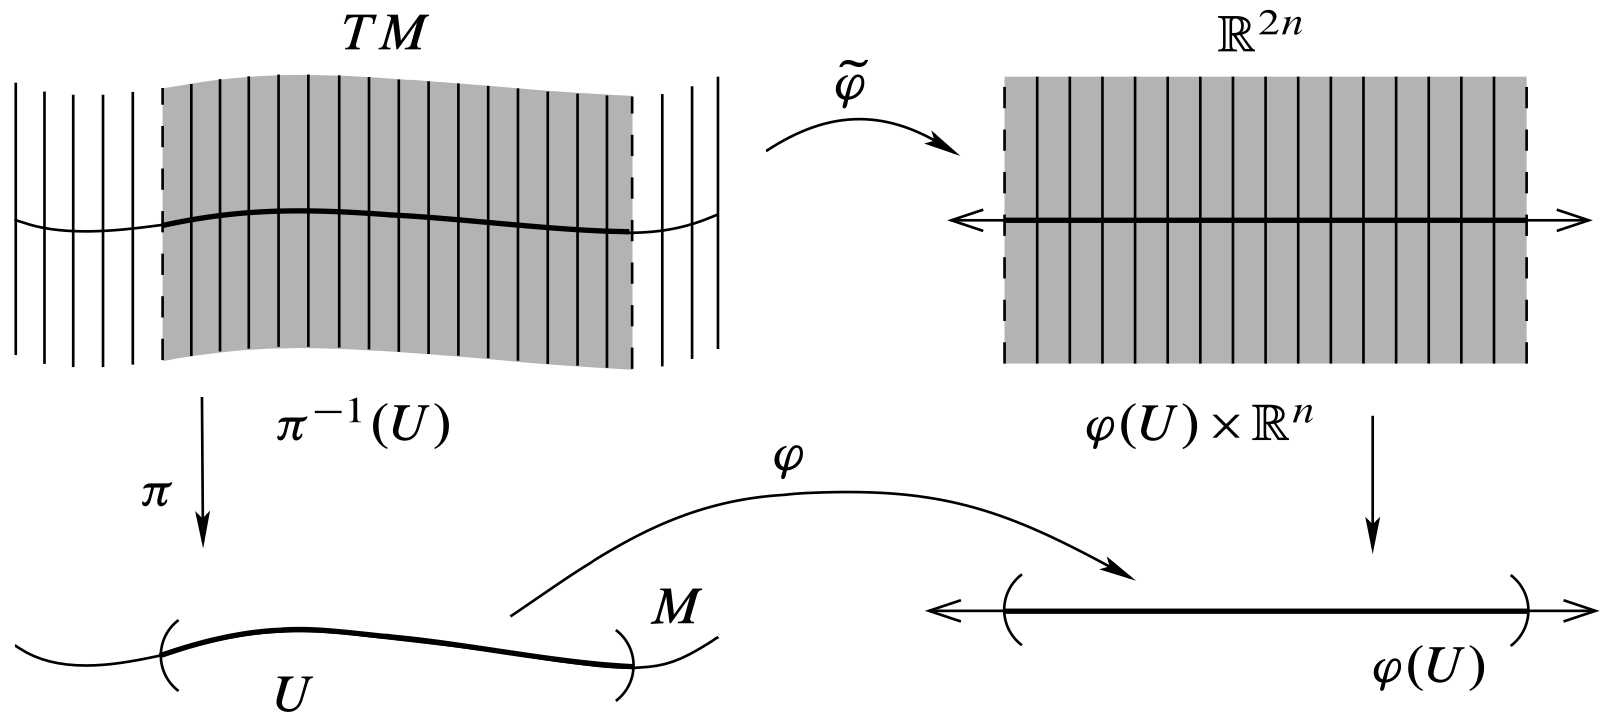
\includegraphics[width=1.8\textwidth]{figs/bundle.png}
	\end{center}
	\caption{Coordinates for the tangent bundle ($\psi_\alpha$ is called $\tilde\varphi$ in the figure)}
\end{marginfigure}
Let $(x^1,\cdots,x^n)$ denote the coordinate functions of $\varphi$, and define\\ the map $\psi_\alpha:V_\alpha\to\R^{2n}$ acting on $v=v^ie_i|_p$ as
$$
\psi_\alpha(v) = (\ub{x^1(p),\cdots,x^n(p)}{\varphi_\alpha(\pi(v))},\ub{v^1,\cdots,v^n}{(\varphi_\alpha)_*v}).
$$
Its image is $\varphi_\alpha \cross \R^n$, which is an open subset of $\R^{2n}$. It is a bijection, because its image can be written as
$$
\psi_\alpha^{-1}(\varphi_\alpha(\pi(v)),(\varphi_\alpha)_*v) = v\Big|_{\varphi^{-1}(x)}.
$$
This proves that $\psi_\alpha$ is a homeomorphism whos domain is all of $TM$, thus a chart. For more on the topology of $TM$ satisfying conditions of the smooth manifold chart lemma, see Ref [3], Pg 21, 67, also Ref [1] Pg 180.\\\\
To see that $\pi$ is smooth, note that w.r.t charts $(U_\alpha,\varphi_\alpha)$ on $M$ and $(V_\alpha,\psi_\alpha)$ on $TM$, its coordinate representation is $\pi(x,v) = x$.


\begin{definition}
	A \tb{section} of $E$ is a continuous map $\sigma:M\to E$ satisfying $\pi \circ \sigma = \id_M$. This means that $\sigma(p)$ is an element of the fiber $E_p$ for each $p \in M$. When $\sigma$ is defined on all of $M$ it is called a \emph{global section}. Sections of $TM$ are precisely vector fields on $M$.\\\\
	The \tb{zero section} of $E$ is the global section $\zeta:M\to E$ defined by
	$$
	\zeta(p) = 0 \in E_p \text{ for each } p \in M
	$$
\end{definition}


\begin{example}
	Given bundles $\pi:E\to M$ and $\pi^\prime:E^\prime\to M^\prime$, show that the maps $\psi:E\to E^\prime$ and $\phi:M\to M^\prime$ are a bundle morphism if and only if $\pi^\prime \circ \psi = \phi \circ \pi$. This condition is shown in Fig 4, where we have drawn the total spaces $E$ and $E^\prime$ over the corresponding base space $M$ and $M^\prime$. Show that $\psi$ uniquely determines $\phi$.
\end{example}
\sol If we set the projection map to the inverse of the zero section $\pi = \zeta^{-1}$, we get
$$
\begin{aligned}
	\phi &= \pi^\prime \circ \psi \circ \pi^{-1}\\
	\Rightarrow \phi &= (\zeta^\prime)^{-1} \circ \psi \circ \zeta
\end{aligned}
$$
We can always say that our base spaces $M, M^\prime$ are the domains of their zero sections. Since we have chosen our manifolds in such a way, $\psi$ uniquely determines $\phi$.


\begin{example}
	Check that $\phi_*$ is smooth when we make the tangent bundle into a manifold as in the previous exercise.
\end{example}
\sol From Ex \ref{b2e55} we know that projection maps are smooth. So setting $\psi=\phi_*$ we have
$$
\phi_* = (\pi^\prime)^{-1} \circ \phi \circ \pi
$$
is smooth if $\phi$ is smooth. Without loss of generality we can set $\phi = \id_M$ so that $M$ and $M^\prime$ are the same, and all maps are smooth in this case.


\begin{example}
	Show that if $\phi:M\to M^\prime$ is a diffeomorphism, then $\phi_*:TM\to TM^\prime$ is a bundle isomorphism.
\end{example}
\sol When $\phi$ is an isomorphism, the dimensions of $M$ and $M^\prime$ are equal, and the spaces $T_pM$ and $T_{\phi(p)}M^\prime$ are isomorphic. Since $\phi_*$ is smooth and linear, it is an isomorphism of the tangent spaces and hence a bundle isomorphism.


\begin{example}\label{b3e59}
	Show that for any manifold $M$, the tangent bundle $\pi:TM\to M$ is locally trivial.
\end{example}
\sol By choosing the standard fiber $F$ to be $\R^n \cong T_pM$ where $n = \dim(T_pM)$, we can always construct a tangent bundle that is locally trivial. This is because the base space $M$ is a manifold (locally Euclidean) and the total space $E \cong M \cross \R^n$.


\begin{example}
	Describe a bundle that is not locally trivial.
\end{example}
\sol Check Ref [20].


\begin{example}
	Check that the tangent bundle of a manifold is a vector bundle.
\end{example}
\sol From Ex \ref{b3e59}, we can always find a locally trivial bundle over a manifold $M$. Furthermore we can assign the pushforward of the chart maps as the local trivialization, which is linear.


\begin{example}\label{b2e62}
	A 1-dimensional bundle is called a (real or complex) \tb{line bundle}. Check that the Möbius strip is a real line bundle if we regard the standard fiber as being $\R$.
\end{example}
\sol First we define an equivalence relation on $\R^2$ by declaring that $(x,y) \sim (x+n,(-1)^ny)$ for some $n \in \Z$. We denote:
\begin{itemize}
	\item The Möbius \emph{band} as the quotient space $E = \R^2 / \sim$, and $q:\R^2 \to E$ is the quotient map.
	\begin{marginfigure}
		\begin{tikzcd}
			\R^2 \arrow[r, "q"] \arrow[d, "\pi_1"]
			& E \arrow[d, "\pi"] \\
			\R \arrow[r, "\varphi"]
			& S^1
		\end{tikzcd}
		\caption{Commutative diagram of the Möbius bundle morphism}
	\end{marginfigure}	
	\item The Möbius \emph{strip} as the finite version, by substituting for one of the real lines a closed interval, $E = ([0,1] \cross \R) / \sim$. The restriction of $q$ to this subset of $\R^2$ is closed and surjective, also a valid quotient map.
\end{itemize}
In both cases $\pi_1$ is the projection map onto the first factor and $\varphi: \R \to S^1$ is the smooth covering map $\varphi(x) = e^{2\pi\di x}$. We have that $\pi:E\to S^1$ is a smooth real line bundle over $S^1$, called the Möbius \emph{bundle}. This is because we can construct from an open subset $U \subseteq S^1$ a local trivialization from $\pi^{-1}(U)$ to $U \cross \R$, with $\R$ as the standard fiber.\marginnote{Ref [3], Pg 251}


\begin{example}
	Show that if a vector bundle morphism is a diffeomorphism, its inverse is a vector bundle morphism.
\end{example}
\sol By definition a diffeomorphism is bijective and has a smooth inverse map. In this case $\phi^{-1}:E^\prime \to E$ would be a vector bundle morphism whos restriction to each fiber $E_p^\prime$ of $E^\prime$ would also be linear.


\begin{example}\label{b2e64}
	Show that a section of the tangent bundle is a vector field.
\end{example}
\sol A section is a function $\sigma:M\to E$ assigns to each point in the base space a vector in the fiber over that point:
$$
\sigma(p) = (p,f(p)) \in E_p
$$
for some $f:M\to F$, where $F$ is the standard fiber. For tangent bundles $TM$, this $F$ is the tangent space $T_pM$. A vector field on $M$ is defined to be a function $v:C^\infty(M) \to C^\infty(M)$. At first glance they seem different, it should instead be $v:C^\infty(M) \to C^\infty(M^\prime)$ where $\dim(M) = \dim(M^\prime)$. The rough idea is that we make the fibers the tangent spaces to each point and then by taking a section, we pick one vector from each tangent space, giving us a vector field. TODO make this rigorous.


\begin{example}
	Show that $\Gamma(E)$ is a module over $C^\infty(M)$.
\end{example}
\sol From Ex \ref{b2e64}, $\Gamma(E) \cong \text{Vect}(M)$ when $E = TM$, but we need to do this for general $E$. From Ex \ref{b1e8} we know that Vect$(M)$ is a module over $C^\infty(M)$, and we can show that $\Gamma(E)$ satisfies all the rules of a $C^\infty(M)$ module like Vect$(M)$ would.


\begin{example}
	Show that every section of the Möbius strip (viewed as a real line bundle over $S^1$) vanishes somewhere. Conclude that the Möbius strip has no basis of sections, hence it is not trivial.
\end{example}
\sol From Ex \ref{b2e62}, we recase the total space as $E = ([0,2\pi] \cross \R) / \sim$ using the equivalence relation $(x,y) \sim (x+2\pi n,(-1)^ny)$ for some $n \in \Z$. We state that $y = \varphi(x)$. We see that the section at $x=0$
$$
\begin{aligned}
	\sigma(0) &= (0, \varphi(0)) = (0, 1)\\
	\sigma(2\pi) &= (2\pi, -\varphi(0))\\
	&= (0, -1)\marginnote{By identifying $n=0$ with $n=1$}\\
	\Rightarrow \sigma(0) = -\sigma(2\pi) = -\sigma(0) = 0
\end{aligned}
$$
and because there is no unique basis to represent zero, there is no basis of sections $\Rightarrow$ Möbius bundle $\pi:E\to S^1$ is not trivial.\\\\
Another way to show only that the Möbius bundle is non-trivial: it is not isomorphic to the trivial bundle $\pi^\prime:S^1\cross \Z_2 \to S^1$. Check Ref [21] Apr 10 notes.


\begin{example}\label{b2e67}
	Check the above statement.\mn{Check that we can make $E^*$ into a manifold so that there is a local trivialization of $E^*$ that is fiberwise linear.} Also, show that given a basis of sections $e_i$ of a vector bundle $E$, there is a unique \tb{dual basis} $e^i$ of sections of $E^*$ such that for each point $p \in M$, $e^i(p)$ is the basis of $E^*_p$ dual to the basis $e_i(p)$ of $E_p$.
\end{example}
\sol Since $E^*$ is the disjoint union of all $E_p^*$, $E$ and $M$ being manifolds makes $E^*$ into a manifold. The local trivialization of $E^*$ for a neighborhood $U$ of $p \in M$ will be similar to that for $E$
$$
\phi:E^*|_U \to U \cross \R^n\marginnote{The following may be useful here:$$(\R^n)^* = \R^n$$}
$$
and $e^i$ is the basis of sections of $E^*$ by construction.


\begin{example}
	Show that if $s$ is a section of a vector bundle $E$ over $M$ and $\lambda$ is a section of $E^*$, there is a smooth function $\lambda(s)$ on $M$ given by
	$$
	\lambda(s)(p) = \lambda(p)(s(p))
	$$
	for all $p\in M$. Show that $\lambda(s)$ depends $C^\infty(M)$-linearly on $\lambda$ and $s$.
\end{example}
\sol We also have that $\lambda$ is a (rough) covector field by duality in Ex \ref{b2e67},\marginnote{Ref [3], Pg 278} because $s$ is a vector field. Writing $\lambda=\lambda_ie^i$ and $s=s^ie_i$, we can form a function $\lambda(s): M \to \R$ which has the coordinate representation
$$
\lambda(s) = \lambda_ie^i(s^je_j) = \lambda_is^j\delta_j^i = \lambda_is^i
$$
which gives us the desired property $\lambda(s)(p) = \lambda(p)(s(p))$ for $p\in M$.


\begin{example}
	Show that a section of the cotangent bundle is the same as a 1-form.
\end{example}
\sol A section of the cotangent bundle provides a map that assigns a covector (linear functional) to each point in the manifold. A 1-form also achieves the same outcome by associating a linear functional with each point that acts on tangent vectors. Since both concepts describe the same functionality with the additional requirement of smoothness, they are essentially equivalent.


\begin{example}
	Check this fact.\mn{$E\oplus E^\prime$ and $E\otimes E^\prime$ have well-defined fibers over $p$.}
\end{example}
\sol The projection map $\pi$ sends $E\oplus E^\prime$\marginnote{Also called the \tb{Whitney sum} as in Ref [3] Pg 254} to $p$. If $\phi$ is a local trivialization of $E\to M$ and $\psi$ is a local trivialization of $E^\prime\to M$, then $(\phi,\psi)$ is a local trivialization of $E\oplus E^\prime$ according to
$$
(\phi,\psi)|_U(q) = (p,(a,b))
$$
where $\pi(q)=p,\phi|_U(q)=(p,a),\psi|_U(q)=(p,b)$. Since $(a,b)$ belongs to the fiber over $p$, both $a$ and $b$ must be evaluated at $p$. This means $a$ is an element of $E_p$ and $b$ is an element of $E_p^\prime$.\\\\
Now consider an element in $(E\otimes E^\prime)_p$\marginnote{See Ref [3] Pg 316 for a general construction of the tensor product vector bundle} which is a tensor product $a \otimes b$ of sections. Since $a \otimes b$ belongs to the fiber over $p$, both sections used for the tensor product must be evaluated at $p$. This means $a$ is an element of $E_p$ and $b$ is an element of $E_p^\prime$.\\\\
This shows $E\oplus E^\prime$ over $M$ has fiber over $p$: $E_p\oplus E_p^\prime$. Likewise, $E\otimes E^\prime$ over $M$ has fiber over $p$: $E_p\otimes E_p^\prime$.


\begin{example}\label{b2e71}
	Suppose that $E$ and $E^\prime$ are vector bundles over $M$, $s$ is a section of $E$, and $s^\prime$ is a section of $E^\prime$. Show that there is a unique section $(s,s^\prime)$ of $E \oplus E^\prime$ such that for each point $p \in M$, $(s,s^\prime)(p) = (s(p),s^\prime(p))$. Show that there is a unique section $s \otimes s^\prime$ of $E \otimes E^\prime$ such that for each $p \in M$, $(s \otimes s^\prime)(p) = s(p) \otimes s^\prime(p)$.
\end{example}
\sol Follows from direct sum and tensor product of vector fields.


\begin{definition}
	Let $\mc{I}$ be a set. A collection indexed by $\mc{I}$ is a collection of sets $\br{S_i}_{i\in \mc{I}}$. In other words, the collection contains one set for each element of $\mc{I}$.\\\\
	A \emph{choice function} is a function
	$$
	f:\mc{I}\to\bigcup_{i\in\mc{I}}S_i
	$$
	such that $f(i)\in S_i$ for all $i \in \mc{I}$. The \tb{axiom of choice} states that for any indexed collection of nonempty sets, there exists a choice function.\marginnote{Ref [25]}
\end{definition}


\begin{example}\label{b2e72}
	Suppose that $E$ and $E^\prime$ are vector bundles over $M$. Show that any section of $E \otimes E^\prime$ can be written, not necessarily uniquely, as a locally finite sum of sections of the form $s \otimes s^\prime$, where $s \in \Gamma(E)$ and $s^\prime \in \Gamma(E^\prime)$.
\end{example}
\sol From Ex \ref{b2e71}, every section of $E \otimes E^\prime$ can be uniquely written as $(s \otimes s^\prime)(p) = s(p) \otimes s^\prime(p)$ where $s \in \Gamma(E)$ and $s^\prime \in \Gamma(E^\prime)$. Additionally if there is a basis of sections for $E$ and $E^\prime$, we can say $s = s^ie_i$ and $s^\prime = s^{\prime i}e_i^\prime$, giving us
$$
(s \otimes s^\prime)(p) = \sum_{i,j}s^ie_i(p) \otimes s^{\prime j}e_j^\prime(p)
$$
but this expression is not necessarily unique if $E$ and $E^\prime$ don't have a basis of sections. For vector bundle $E = M \cross F$, only $F$ is required to be an $n$-dimensional vector space. For the standard fiber, $F$ is isomorphic to $\R^n$, which always has a basis\marginnote{Ref [6] Pg 148}. Assuming the axiom of choice, every vector space admits a Hamel basis.\marginnote{Ref [22] Pg 33}


\begin{example}
	Suppose that $E$ is a vector bundle over $M$. Define the \tb{exterior algebra bundle} $\Lambda E$ over $M$ to have the total space equal to the union of the vector spaces $\Lambda E_p$ and projection map $\pi$ sending $\Lambda E_p$ to $p$. Show how to make $\Lambda E$ into a manifold such that $\pi:\Lambda E \to M$ is a vector bundle.
\end{example}
\sol TODO


\begin{example}
	Show that $\Lambda E$ is the direct sum of bundles $\Lambda^i E$,
	$$
	\Lambda E = \bigoplus_{i=0}^{n} \Lambda^i E
	$$
	where $n$ is the dimension of the fibers of $E$, and the vector bundle $\Lambda^i E$ has fiber over $p\in M$ given by $\Lambda^i E_p$. Show that sections of $\Lambda^0 E$ are in natural one-to-one correspondence with functions on $M$ and sections of $\Lambda^1 E$ are in natural one-to-one correspondence with sections of $E$.
\end{example}
\sol TODO


\begin{example}
	Show that for any sections $\omega,\mu$ of $\Lambda E$ there is a section $\omega \wedge \mu$ given by
	$$
	(\omega \wedge \mu)(p) = \omega(p) \wedge \mu(p).
	$$
	Show that the sections of $\Lambda E$ form an algebra. Show that the sections of $\Lambda^i E$ form a subspace of the sections of $\Lambda E$, and that the sections of $\Lambda^i E$ are all locally finite sums of wedge products of sections of $E$.
\end{example}
\sol TODO


\begin{example}
	Show that sections of $\Lambda^i T^*M$ are in natural one-to-one correspondence with $i$-forms on $M$.
\end{example}
\sol TODO


\begin{example}
	Show that these conditions imply $g_{\alpha\beta} = g_{\beta\alpha}^{-1}$. Show that for any sequences $\alpha_1,\cdots,\alpha_n$ and $\beta_1,\cdots,\beta_m$ with $\alpha_1 = \beta_1$, $\alpha_n = \beta_m$, they imply
	$$
	g_{\alpha_1\alpha_2}\cdots g_{\alpha_{n-1}\alpha_n} = g_{\beta_1\beta_2}\cdots g_{\beta_{m-1}\beta_m}.
	$$ 
\end{example}
\sol Taking two transition functions $g_{\alpha\beta}$ and $g_{\beta\alpha}$ and composing them should yield $\id$ because we do not identify two different points in the same trivial bundle. So
$$
g_{\beta\alpha}g_{\alpha\beta} = \id\Rightarrow g_{\beta\alpha} = g_{\alpha\beta}^{-1}
$$
Equivalently, if we have two sequences of transition functions that start at the same bundle and end at the same bundle, they should yield the same transition function.


\begin{example}
	Prove that if $g_{\alpha\alpha} = 1$ and $g_{\alpha\beta}g_{\beta\gamma}g_{\gamma\alpha} = 1$ where defined, $\pi:E\to M$ is a vector bundle. (Hint: first show how to give each fiber $E_p$ the structure of a vector space, and then show that $E$ is trivial over each set $U_\alpha$, with a fiberwise linear local trivialization.)
\end{example}
\sol This actually shown on Pg 214, right after the exercise.


\begin{example}
	Show that if the above condition holds\mn{$$[p,v]_\alpha \mapsto [p,d\rho(x)v]_\alpha$$}, and $p \in U_\alpha \cap U_\beta$, then $T$ is also of the form
	$$
	[p,v^\prime]_\beta \mapsto [p,d\rho(x^\prime)v^\prime]_\beta
	$$
	for some $v^\prime \in \mf{g}$.
\end{example}
\sol The first condition comes from the fact that just as every Lie group has a Lie algebra, every homomorphism $\rho:G\to H$ between Lie groups determines a corresponding homomorphism $d\rho:\mf{g}\to \mf{h}$ between their Lie algebras.\\\\
The second condition holds if we define $v^\prime = g_{\beta\alpha}v$ and $d\rho(x^\prime) = g_{\beta\alpha}d\rho(x)g_{\beta\alpha}^{-1}$.


\begin{example}
	Check that if $\phi:\R^4\to\C^3$ is a solution of this equation, so is $U_1(g)\phi$ for any $g\in\SU(2)$.
\end{example}
\sol We may rewrite the equation as follows:
$$
\sparen{(\partial^\mu\partial_\mu+m^2) + \lambda \ub{\phi^i\phi_i}{\ip{\phi}}}\phi=0
$$
Now the unitary group SU$(2)$ preserves the inner product, and its representation $U_1$ is simply a rotation. To see why:
$$\begin{aligned}
	\ip{U_1(g)\phi}&=\phi^*U_1^*(g)U_1(g)\phi\\&=\phi^*\cancel{U_1^{-1}(g)U_1(g)}\phi\\&=\ip{\phi}
\end{aligned}
$$
So
$$
\begin{aligned}
	\sparen{(\partial^\mu\partial_\mu+m^2) + \lambda \ip{U_1(g)\phi}}U_1(g)\phi&=0\\
	\sparen{(\partial^\mu\partial_\mu+m^2) + \lambda \phi^i\phi_i}U_1(g)\phi&=0
\end{aligned}
$$
making $U_1(g)\phi$ another valid solution.


\begin{marginfigure}
	\begin{center}
	  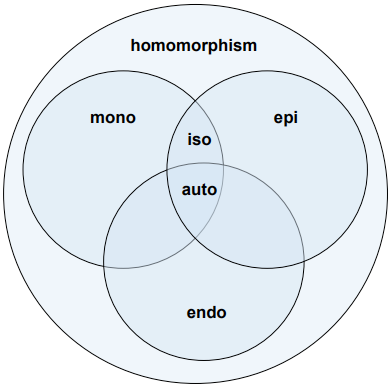
\includegraphics[width=1.2\textwidth]{figs/morphism.png}
	\end{center}
	\caption{Morphisms}
\end{marginfigure}
\begin{definition}
	\tb{Morphisms:}
	\begin{itemize}
		\item Homomorphism: preserves group structure
		\item Epimorphism: surjective, onto
		\item Monomorphism: injective, 1-1
		\item Isomorphism: bijective, 1-1 and onto
		\item Endomorphism: from a structure to itself
		\item Automorphism: bijective endomorphism
	\end{itemize}
\end{definition}


\begin{example}
	Show this.\mn{All $C^\infty(M)$-linear maps $T:\Gamma(E)\to\Gamma(E)$ correspond to sections of End$(E)$.} (Hint: use a local trivialization and the `partition of unity' trick described in Sec \ref{b1c6} to reduce this to the case of a trivial bundle.)
\end{example}
\sol TODO


\begin{example}
	Show that the product or inverse of gauge transformations is a gauge transformation, and that the identity is a gauge transformation.
\end{example}
\sol Suppose that $S,T \in \text{End}(E)$ are gauge transformations, and we know from Pg 220 of the text that End$(V)$ is an algebra, so that the \underline{product} $ST$ is also a gauge transformation.\\\\
An endomorphism that is also bijective (automorphisms $\text{Aut}(E) \subset \text{End}(E)$) would have an \underline{inverse}. In this case we have closure within Aut$(E)$ making it also a gauge transformation.\\\\
The \underline{identity} is a gauge transformation because $\id \in \text{End}(E)$.


\begin{example}
	Check that $A(v)$ is well-defined, i.e., independent of how we write $A$ as a sum $\sum_i T_i \otimes \omega_i$.
\end{example}
\sol Let's write $A(v)$ in two ways
$$
A(v) = \sum_i \omega_i^\prime(v) \p*{\sum_{j,k} T_i^j (e_j \otimes e^k)} = \sum_i \omega_i^\prime(v) \p*{\sum_{j,k} T_i^j (f_j \otimes f^k)}
$$
where $T_i$ is expanded using two different sets of basis of sections over End$(E)$. $A(v)s$ will be the same section on $E$ no matter what basis is chosen.


\begin{example}
	Work out the details of the proof we have sketched here.\mn{Proving the claim that any connection $D$ can be written as $D=D^0+A$, where $D^0$ is called the \tb{standard flat connection} on $E|_U$ and $A$ is called the \tb{vector potential}, an End$(E)$-valued 1-form.}
\end{example}
\sol We check the connection laws on $D=D^0+A$ such that
$$
D_v(s) = D_v^0(s) + A(v)(s)
$$
is the action of $D_v$ on a section $s$ of $E$:
\begin{enumerate}
	\item $D_v(\alpha s) = D_v^0(\alpha s) + A(v)(\alpha s) = \alpha D_v^0(s) + \alpha A(v)(s) = \alpha D_v(s)$
	\item $D_v(s + t) = D_v^0(s+t) + A(v)(s+t) = D_v^0(s) + A(v)(s) + D_v^0(t) + A(v)(t) = D_v(s) + D_v(t)$
	\item $D_v(fs) = v(f)s+fD_v(s)$\marginnote{Pg 227 of the text}
	\item $D_{v+w}(s) = D_{v+w}^0(s) + A(v+w)(s) = D_v^0s + A(v)s + D_w^0s + A(w)(s) = D_vs + D_ws$
	\item $D_{fv}s = D_{fv}^0(s) + A(fv)(s) = fD_v^0s + fA(v)s = fD_vs$
\end{enumerate}
The only remaining thing to check is the statement $A(\partial_\mu)e_j = A_{\mu j}^i e_i$ which follows from the general calculation on Pg 225 of $A(v)s$ where $v=v^\mu \partial_\mu$ and $s=s^j e_j$. Here all the vector and section components are set to 1.


\begin{example}
	Check that $D^\prime$ has the rest of the properties of a connection.
\end{example}
\sol We check the connection laws on $D_v^\prime(s) = gD_v(g^{-1}s)$:\marginnote{Here we make the implicit assumption that $f$ commutes with gauge transformation $g$ (?)}
\begin{enumerate}
	\item $D_v^\prime(\alpha s) = gD_v(\alpha g^{-1}s) = \alpha gD_v(g^{-1}s) = \alpha D_v^\prime(s)$
	\item $D_v^\prime(s + t) = gD_v(g^{-1}(s+t)) = gD_v(g^{-1}s) + gD_v(g^{-1}t) = D_v^\prime(s) + D_v^\prime(t)$
	\item $D_v^\prime(fs) = v(f)s+fD_v^\prime s$\marginnote{Pg 229 of the text}
	\item $D_{v+w}^\prime(s) = gD_{v+w}(g^{-1}s) = gD_v(g^{-1}s) + gD_w(g^{-1}s) = D_v^\prime(s) + D_w^\prime(s)$
	\item $D_{fv}^\prime s = gD_{fv}(g^{-1}s) = gfD_v(g^{-1}s) = fgD_v(g^{-1}s) =  fD_v^\prime s$
\end{enumerate}


\begin{example}
	Using a local trivialization of $E$ over $U_\alpha \subseteq M$ write the $G$-connection $D$ as the standard flat connection plus a vector potential: $D=D^0+A$. Show that the vector potential $A^\prime$ for $D^\prime$ is given in local coordinates by
	$$
	A_\mu^\prime = gA_\mu g^{-1} + g\partial_\mu g^{-1}.
	$$
	Show that since $A_\mu$ lives in $\mf{g}$, so does $A_\mu^\prime$. (Hint: show that if $A_\mu$ lives in $\mf{g}$ and $g\in G$, then $gA_\mu g^{-1}$ lives in $\mf{g}$. Also show that if $g\in \mc{G}$, then $g\partial_\mu g^{-1}$ lives in $\mf{g}$.) Conclude that $D^\prime$ is a $G$-connection.
\end{example}
\sol Let's see how the gauge transformed connection affects the vector potential by applying it to a section $s$:
$$
\begin{aligned}
	D_v^\prime(s) &= gD_v(g^{-1}s)\\
	&= gD_v^0(g^{-1}s) + gA(v)(g^{-1}s)\\
	&= gv(g^{-1}s) + \cancel{gg^{-1}}D_v^0(s)+ gA(v)(g^{-1}s)\marginnote{Leibniz}\\
	&= D_v^0(s) + gv^\mu A(\partial_\mu)(g^{-1}s) + gv^\mu\partial_\mu(g^{-1}s)\marginnote{Reorder terms, set $v=v^\mu\partial_\mu$}\\
	&= D_v^0(s) + v^\mu gA_\mu(g^{-1}s) + v^\mu g\partial_\mu(g^{-1}s)\marginnote{$g$ commutes with local coordinate functions\\\\$x^\mu$, and $f(\partial_\mu) = f_\mu$ is a simpler notation, see Pg 127 of the text}\\
	&= D_v^0(s) + v^\mu \ub{\p*{\ub{gA_\mu g^{-1}}{(1)} + \ub{g\partial_\mu g^{-1}}{(2)}}}{A_\mu^\prime}s\\
	&= D_v^0(s) + A^\prime(v)s
\end{aligned}
$$
$A_\mu^\prime$ lives in $\mf{g}$ if for the two terms above:
\begin{enumerate}
	\item $A_\mu$ lives in $\mf{g}$ and $g \in G \subset \mc{G}$, i.e, $G$ is a gauge transformation $\Rightarrow$ $gA_\mu g^{-1}$ lives in $\mf{g}$
	\item $g \in \mc{G}$ $\Rightarrow$ $g\partial_\mu g^{-1}$ lives in $\mf{g}$
\end{enumerate}
When these conditions are satisfied, $D^\prime$ is a $G$-connection $\Rightarrow$ $G$ and $G^\prime$ are gauge-equivalent.


\begin{example}
	Suppose that $E$ is a trivial $G$-bundle over the spacetime $\R \cross S$ where $S$ is any manifold. Given an End$(E)$-valued 1-form $A$ on $M$, let $A_0=A(\partial_t)$, where $t$ is the usual time coordinate on $\R \cross S$. We say that a $G$-connection $D$ on $E$ is in \tb{temporal gauge} if $D=D^0+A$ where $A_0=0$. Modify the argument given in the section on gauge freedom in Sec \ref{b1c6} to show that any $G$-connection on $E$ is gauge-equivalent to one in temporal gauge.
\end{example}
\sol TODO
%From Pg 128, 230 of the text, $A^\prime=A-df$


\begin{example}\label{b2e88}
	Show that $D_{\gamma^\prime(t)}u(t)$ defined in this manner\mn{The \tb{covariant derivative} is$$D_{\gamma^\prime(t)}u(t)=\frac{d}{dt}u(t)+A(\gamma^\prime(t))u(t).$$} is actually independent of the choice of local trivialization.
\end{example}
\sol Check Ref [23] Pg 50 for a proof that $\nabla_XY|_p$ depends only on the value of $X$ and $Y$ in an arbitrarily small neighborhood of $p$. By Pg 57, this formulation is equivalent to the covariant derivative on curves that we see here.


\begin{definition}
	For any metric space $X$, we can define a norm on the vector space $C_\infty(X)$ (the set of all functions $f:X\to\C$ such that $f$ is continuous and bounded) via
	$$
	\norm{u}_\infty=\sup_{x\in X} \abs{u(x)}.
	$$
	And now that we have a norm, we can think about convergence in that norm: we have $u_n \to u$ in $C_\infty(X)$ (convergence of the sequence) if
	$$
	\lim_{n\to\infty} \norm{u_n-u}_\infty=0,
	$$
	which is the definition of \tb{uniform convergence} on $X$.
\end{definition}


\begin{example}
	Put a norm on the vector space $V$ and give End$(V)$ the norm
	$$
	\norm{T} = \sup_{\norm{u}=1}\norm{Tu}.
	$$
	Let
	$$
	K=\sup_{t\in[0,t]}\norm{A(\gamma^\prime(t))}.
	$$
	Show that the $n$th term in the sum above has norm $\le t^nK^n\norm{u}/n!$, so that the sum converges. Show using similar estimates that $u(t)$ is differentiable (in fact, smooth), and that $u(0)=u$ and $\frac{d}{dt}u(t)=-A(\gamma^\prime(t)u(t))$.
\end{example}
\sol The infinite sum, where $u=u(0)$
$$
u(t)=\sum_{n=0}^{\infty}\ub{\p*{(-1)^n\int_{t\ge t_1\ge \cdots \ge t_n\ge 0}A(\gamma^\prime(t_1))\cdots A(\gamma^\prime(t_n))dt_n\cdots dt_1}}{T}u
$$
has $n$th term (call this $T_n$), with norm equal to
$$
\begin{aligned}
	\norm{T_n} &= \sup_{\norm{u}=1}\norm{Tu}\\
	&= \norm{(-1)^n\int_{0}^{t}\int_{0}^{t_1}\cdots\int_{0}^{t_{n-1}}A(\gamma^\prime(t_1))\cdots A(\gamma^\prime(t_n))dt_n\cdots dt_1 u}\\
	&= \int_{0}^{t}\int_{0}^{t_1}\cdots\int_{0}^{t_{n-1}}\norm{A(\gamma^\prime(t_1))\cdots A(\gamma^\prime(t_n)) u} dt_n\cdots dt_1 \\
	&\le \int_{0}^{t}\int_{0}^{t_1}\cdots\int_{0}^{t_{n-1}}\norm{A(\gamma^\prime(t_1))\cdots A(\gamma^\prime(t_n))}\norm{u}dt_n\cdots dt_1 \marginnote{Submultiplicativity of this norm (?)}\\
	&\le \int_{0}^{t}\int_{0}^{t_1}\cdots\int_{0}^{t_{n-1}} K^n \norm{u} dt_n\cdots dt_1\\
	&= \int_{0}^{t}\int_{0}^{t_1}\cdots\int_{0}^{t_{n-2}} K^n \norm{u} t_{n-1}dt_{n-1}\cdots dt_1\\
	&= \int_{0}^{t}\int_{0}^{t_1}\cdots\int_{0}^{t_{n-3}} K^n \norm{u} \frac{t_{n-2}^2}{2}dt_{n-2}\cdots dt_1\\
	% &= \int_{0}^{t}\int_{0}^{t_1}\cdots\int_{0}^{t_{n-4}} K^n \norm{u} \frac{t_{n-2}^3}{2\cdot 3}dt_{n-3}\cdots dt_1\\
	&\vdots\\
	&= \frac{t^nK^n\norm{u}}{n!}\\
	\Rightarrow \norm{u(t)} &\le \sum_{n=0}^{\infty} \frac{t^nK^n\norm{u}}{n!} = \norm{u}\exp(tK)
\end{aligned}
$$
which means the sequence $\{u(t_i)\}$ for $t_i \in \sparen{0,t}$ is uniformly convergent.\\\\
Since $n!$ can be infinitely differentiable using the Gamma function, setting $n=0$ recovers the original boundary conditions because we integrate directly from 0 to $t$.


\begin{example}
	Let $\alpha:[0,T]\to M$ be a piecewise smooth path and let $f:[0,S]\to [0,T]$ be any piecewise smooth function with $f(0)=0,f(S)=T$. Let $\beta$ be the reparametrized path given by $\beta(t)=\alpha(f(t))$. Show that for any connection $D$ on a vector bundle $\pi:E\to M, H(\alpha,D)=H(\beta,D)$.
\end{example}
\sol To show that holonomy is invariant under reparametrization, we need to demonstrate that the parallel transport of a vector along a piecewise smooth path is independent of the parameterization of the path. Let $s \in \Gamma(E)$
$$
	0 = D_{\beta^\prime(t)}s = D_{f^\prime(t)\alpha^\prime(f(t))}s = f^\prime(t)\ub{D_{\alpha^\prime(f(t))}s}{0} = 0
$$
because $D_{fv}s = fD_vs$.


\begin{example}\label{b2e91}
	Check these identities.\mn{Holonomy identities on paths}
\end{example}
\sol Using the path-ordered exponential, we express:
$$
H(\gamma,D)u=u(t)=\mc{P}e^{-\int_{0}^{t}A(\gamma^\prime(s))ds}u.
$$
\begin{itemize}
	\item From the definition of product path on Pg 238 of the text$$
	\begin{aligned}
		H(\beta\alpha,D) &= \mc{P}\exp\p*{-\int_{0}^{S+T}A((\beta\alpha)^\prime(s))ds}\\
		&= \mc{P}\exp\p*{-\int_{0}^{S}A(\alpha^\prime(s))ds-\int_{S}^{S+T}A(\beta^\prime(t-S))ds}\\
		&= \mc{P}\exp\p*{-\int_{0}^{S}A(\alpha^\prime(s))ds}\exp\p*{-\int_{S}^{S+T}A(\beta^\prime(s-S))ds}\marginnote{Split exponential and reorder}\\
		&= \mc{P}\exp\p*{-\int_{0}^{S}A(\alpha^\prime(s))ds}\exp\p*{-\int_{0}^{T}A(\beta^\prime(s))ds}\marginnote{Reparametrize second integral from $s-S\to s$}\\
		&= H(\beta,D)H(\alpha,D)\marginnote{Uses meta-operator $\mc{P}$}
	\end{aligned}$$
	\item $H(\id_p,D)=\mc{P}e^{-\int_{0}^{t}A(\id^\prime(s))ds} = e^0 = \id$
	\item If we reverse the direction of the curve, we reverse the tangent vector, so $A\to-A$:\marginnote{Ref [1], Pg 219, Ex 8.23}
	$$
	\begin{aligned}
		\mc{P}e^{\int_{0}^{t}A(\gamma^\prime(s))ds} &= \p*{\mc{P}e^{-\int_{0}^{t}A(\gamma^\prime(s))ds}}^{-1}\\
		\Rightarrow H(\gamma^{-1},D) &= H(\gamma,D)^{-1}
	\end{aligned}
	$$
	\item $H(\id_q\alpha,D) = H(\id_q,D)H(\alpha,D) = H(\alpha,D)$
	\item $H(\alpha \id_p,D) = H(\alpha,D)H(\id_p,D) = H(\alpha,D)$
\end{itemize}


\begin{example}
	Check that this formula holds even when the path $\gamma$ does not stay within an open set over which we have trivialized the $G$-bundle $E$, by breaking up $\gamma$ into smaller paths.
\end{example}
\sol Let's try out a gauge transformed version of the product path $\beta\alpha$ that straddles two open sets
$$
\begin{aligned}
	H(\beta\alpha,D^\prime) &= H(\beta,D^\prime)H(\alpha,D^\prime)\\
	&= g(\beta(T))H(\beta,D)\ub{g(\beta(0))^{-1}g(\alpha(S))}{\id}H(\alpha,D)g(\alpha(0))^{-1}\marginnote{$\alpha$ and $\beta$ are composable, so \begin{itemize}
		\item $\beta(0) = \alpha(S)$
		\item $\beta(T) = \beta\alpha(S+T)$
		\item $\alpha(0) = \beta\alpha(0)$
	\end{itemize}}\\
	&= g(\beta(T))H(\beta,D)H(\alpha,D)g(\alpha(0))^{-1}\\
	&= g(\beta\alpha(S+T))H(\beta\alpha,D)g(\beta\alpha(0))^{-1}\\
\end{aligned}
$$


\begin{example}
	Show that if $D$ is a $G$-connection on a $G$-bundle and $\gamma$ is a loop, the holonomy $H(\gamma,D)$ lives in $G$. (Hint: first work in a local trivialization and use the fact that $\mf{g}$ is the tangent space of the identity element of $G$.)
\end{example}
\sol The holonomy of a loop is obtained by parallel transporting a point in the fiber around the loop, and is an endomorphism of the fiber. We introduce (informally) the notion of a \emph{principal bundle} where the total space is $E = M \cross G$. Since the fiber is a copy of the gauge group $G$, and the parallel transport preserves the fiber structure, the resulting point must also be in $G$. Therefore, the holonomy is an element of the gauge group $G$.



\newpage
\section{Curvature and the Yang-Mills Equation}\label{b2c3}



\begin{example}
	Check the above identity.
\end{example}
\sol $$
\begin{aligned}
	[v,fw]&=v(fw)-fw(v)\\
	&=v(f)w+\ub{fv(w)-fw(v)}{[\cdot,\cdot]}\marginnote{Pg 26 of text, Leibniz rule for vector fields}\\
	&=f[v,w]+v(f)w
\end{aligned}
$$


\begin{example}\label{b2e95}
	Prove this formula\mn{$$H(\gamma,D)=\id-\epsilon^2F_{\mu\nu}$$} for the holonomy around a small square. (Hint: use the path-ordered exponential formula for parallel transport and keep only terms of order $\epsilon^2$ or less.)
\end{example}
\sol Check Ref [1], Appendix E: Holonomy of an infinitesimal loop.


\begin{example}\label{b2e96}
	Show this\mn{The holonomies along any two homotopic paths from some point $p$ to another point $q$ are the same.}. (Hint: choose a homotopy $\gamma_s$ between two paths $\gamma_0$ and $\gamma_1$ from $p$ to $q$, express the parallel transport map $H(\gamma_s,D)$ using the path-ordered exponential, and show
	$$
	\frac{d}{ds}H(\gamma_s,D)=0
	$$
	if $D$ is flat.)
\end{example}
\sol \underline{First proof:}\\\\
We use the straight-line homotopy from Ex \ref{b1e81}
\begin{marginfigure}
	\begin{center}
		\vspace*{35px}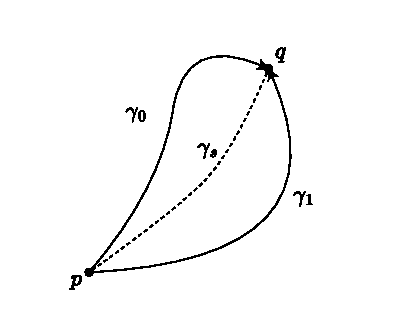
\includegraphics[width=1.4\textwidth]{figs/loop.pdf}
	\end{center}
	\caption{Homotopic paths}
\end{marginfigure}
$$
\gamma_s(t) = (1-s)\gamma_0(t)+s\gamma_1(t)
$$
We check whether holonomy of $\gamma_s$ changes with $s$:
$$
\begin{aligned}
	\frac{d}{ds}H(\gamma_s,D) &= \frac{d}{ds}\mc{P}\exp\p*{-\int_{0}^{t}A(\gamma_s^\prime(s))ds}\\
	&= \frac{d}{ds}\mc{P}\exp\p*{-\int_{0}^{t}A((1-s)\gamma_0^\prime(t)+s\gamma_1^\prime(t))ds}\\
	&= \frac{d}{ds}\mc{P}\exp\p*{-\int_{0}^{t}\sparen{A(\gamma_0^\prime(t))-sA(\gamma_0^\prime(t)-\gamma_1^\prime(t))}ds}\marginnote{$A$ is a linear functional (an End$(E)$-valued 1-form)}\\
	&= \frac{d}{ds}\mc{P}\exp\p*{-t\p{A(\gamma_0^\prime(t))-A(\gamma_0^\prime(0))}+\frac{t^2}{2}\sparen{\p{A(\gamma_0^\prime(t))-A(\gamma_0^\prime(0))}-A(\gamma_1^\prime(t))+A(\gamma_1^\prime(0))}}\\
	&=0
\end{aligned}
$$
We have shown that $H(\gamma_s,D)$ is independent of $s$. So the entire family of homotopic curves $\gamma_s$ has the same holonomy. This argument depends on curvature in that the straight-line homotopy is well defined with a flat connection.\\\\
\underline{Second proof:}\\\\
Let $\gamma = \gamma_1^{-1} \circ \gamma_0$ be the loop from $p$ to $q$ and back. From Ex \ref{b2e95} we know that $H(\gamma,D)=\id-\epsilon^2F_{\mu\nu}$, but on a flat connection we have zero curvature so
$$
\begin{aligned}
	H(\gamma,D) &= \id\marginnote{Rules are in Ex \ref{b2e91}}\\
	\Rightarrow H(\gamma_1^{-1}\gamma_0,D) &= \id\\
	\Rightarrow H(\gamma_1,D)^{-1}H(\gamma_0,D) &= \id\\
	\Rightarrow H(\gamma_0,D) &= H(\gamma_1,D)
\end{aligned}
$$


\begin{example}
	Show that every connection on a vector bundle $\pi:E\to M$ is flat if $M$ is 1-dimensional.
\end{example}
\sol For two vector fields $v=f(x)\partial_x,w=g(x)\partial_x$ on $M$, we use antisymmetry of the curvature to show
$$
\begin{aligned}
	F(v,w) &= -F(w,v)\\
	\Rightarrow f(x)g(x)F(\partial_x,\partial_x) &= -g(x)f(x)F(\partial_x,\partial_x)\\
	\Rightarrow F(v,w) &= 0\marginnote{0-forms $f(x),g(x)$ commute}
\end{aligned}
$$
This converse of the result proved in Ex \ref{b2e96} - namely that if the curvature is zero then we have a flat connection - is a corollary of the Ambrose-Singer theorem, Ref [1] Pg 220.


\begin{example}\label{b2e98}
	Use Ex \ref{b2e72} to show that any $E$-valued differential form can be written - not necessarily uniquely - as a sum of those of the form $s\otimes \omega$, where $s$ is a section of $E$ and $\omega$ is an ordinary differential form on $M$.
\end{example}
\sol Like earlier we can define a basis of sections on $E$ for section $s$ and basis of differential forms for $p$-form $\omega$ and write $s=s^ie_i$ and $\omega=\omega_i (dx^1\wedge\cdots\wedge dx^p)^i = \omega_i w^i$ and write an $E$-valued differential form $\alpha$ as the sum
$$
\alpha = b_j^i (e_i \otimes w^j) = c_l^k (e_k^\prime \otimes w^{\prime l}) \marginnote{As per Einstein notation, we assume $\sum_{i,j}$ and $\sum_{k,l}$ for these two representations of $\alpha$}
$$
where the two bases are related by $e_i = T_i^k e_k^\prime$ and $w^j = S_l^j w^{\prime l}$.


\begin{example}\label{b2e99}
	Using the previous exercise (Ex \ref{b2e98}), show that there is a unique way to define the wedge product of an $E$-valued form $s\otimes \omega$ and the ordinary form $\mu$ is given by
	$$
	(s\otimes \omega) \wedge \mu = s\otimes (\omega \wedge \mu),
	$$
	such that the wedge product depends $C^\infty(M)$-linearly on each factor.
\end{example}
\sol Using $\alpha$ from Ex \ref{b2e98}, then taking the wedge product $\alpha \wedge \mu$, we just use associativity between tensor and wedge products to demonstrate $C^\infty(M)$-linearity.


\begin{example}
	Check that these definitions are equivalent.\mn{$$\begin{aligned}
		d_Ds(v)&=D_vs\\d_Ds&=D_\mu s \otimes dx^\mu
	\end{aligned}$$}
\end{example}
\sol Working out each step in detail:
$$
\begin{aligned}
	d_Ds(v) &= D_\mu s \otimes dx^\mu(v)\\
	&= D_\mu s \otimes dx^\mu(v^\lambda \partial_\lambda)\\
	&= D_\mu s \otimes v^\lambda dx^\mu(\partial_\lambda)\\
	&= D_\mu s \otimes v^\lambda \delta^\mu_\lambda\\
	&= D_\mu s \otimes v^\mu \marginnote{Could get here directly with $df(v)=v(f)$}\\
	&= v^\mu D_\mu s \\
	&= v^\mu D_{\partial\mu} s \marginnote{Explicit notation}\\
	&= D_{v^\mu \partial\mu} s \marginnote{$fD_vs=D_{fv}s$}\\
	&= D_v s \\
\end{aligned}
$$


\begin{example}\label{b2e101}
	Check that the definition above\mn{$$(T\otimes\omega)\wedge(s\otimes\mu)=T(s)\otimes(\omega\wedge\mu)$$} extends uniquely to a wedge product of arbitrary End$(E)$-valued forms and $E$-valued forms that is $C^\infty(M)$-linear in each argument.
\end{example}
\sol We combine Ex \ref{b2e71} and Ex \ref{b2e99} to give the following breakdown:
\begin{itemize}
	\item $T(s)$: This is a section of $E$, as $T$ is an endomorphism mapping sections of $E$ to sections of $E$.
	\item $\omega\wedge\mu$: This is an ordinary differential form.
\end{itemize}
So, the tensor product of a section of $E$ with a differential form is an $E$-valued form. Because tensor and wedge products preserve $C^\infty(M)$-linearity, the result is $C^\infty(M)$-linear in each argument $T,s,\omega,\mu$.


\begin{example}
	Check this identity.
\end{example}
\sol See Ex \ref{b1e24}, proof 3.


\begin{example}\label{b2e103}
	Check that $D^*$ is a connection on $E^*$.
\end{example}
\sol Using the definition of $D^*$ for $v,w \in \text{Vect}(M)$, $s \in \Gamma(E)$, $\lambda,\rho \in \Gamma(E^*)$
$$
[D_v^*\lambda](s)=v(\lambda(s))-\lambda D_v(s)
$$
we use the connection laws for $D$ on Pg 223 of the text to prove them for $D^*$:
\begin{enumerate}
	\item $[D_v^*(\alpha \lambda)](s)=v(\alpha\lambda(s))-\alpha\lambda D_v(s)=\alpha v(\lambda(s))-\alpha\lambda D_v(s)=\alpha[D_v^*(\lambda)](s)$
	\item $[D_v^*(\lambda + \rho)](s) = v((\lambda + \rho)(s))-(\lambda + \rho) D_v(s) = v(\lambda(s))-\lambda D_v(s) + v(\rho(s))-\rho D_v(s) = [D_v^*\lambda](s)+[D_v^*\rho](s)$
	\item $[D_v^*(f\lambda)](s) = v(f\lambda(s))-f\lambda D_v(s) = v(f)\lambda(s)+f(v(\lambda)(s))-f\lambda D_v(s) = v(f)\lambda(s)+f[v(\lambda)-\lambda D_v](s)=v(f)\lambda(s)+f[D_v^*\lambda](s)$
	\item $[D_{v+w}^*(\lambda)](s)=(v+w)(\lambda(s))-\lambda D_{v+w}(s)=v(\lambda(s))-\lambda D_v(s)+w(\lambda(s))-\lambda D_w(s) = [D_v^*\lambda](s)+[D_w^*\lambda](s)$
	\item $[D_{fv}^*\lambda](s) = fv(\lambda(s))-\lambda D_{fv}(s)=fv(\lambda(s))-\lambda fD_v(s) = f[v(\lambda)-\lambda D_v](s)= f[D_v^*\lambda](s)$
\end{enumerate}


\begin{example}
	Check that $D \oplus D^\prime$ is a connection.
\end{example}
\sol We have for
$$
(D \oplus D^\prime)_v(s,s^\prime) = (D_vs,D_v^\prime s^\prime)
$$
that $D,D^\prime$ are connections on $E$ and $E^\prime$ respectively. So the direct sum is a connection.


\begin{example}\label{b2e105}
	Check that $D \otimes D^\prime$ is a connection.
\end{example}
\sol Using the definition
$$
(D \otimes D^\prime)_v(s \otimes s^\prime) = (D_vs)\otimes s^\prime+s\otimes (D_v^\prime s^\prime)
$$
we prove the connection laws for $D \otimes D^\prime$:
\begin{enumerate}
	\item $(D \otimes D^\prime)_v(\alpha s \otimes \beta s^\prime)=(D_v(\alpha s))\otimes \beta s^\prime+\alpha s\otimes (D_v^\prime (\beta s^\prime))=\alpha\beta(D \otimes D^\prime)_v(s \otimes s^\prime)$
	\item $$
	\begin{aligned}
			(D \otimes D^\prime)_v((s+t) \otimes (s^\prime+t^\prime)) &= (D \otimes D^\prime)_v((s\otimes s^\prime)+(s\otimes t^\prime)+(t\otimes s^\prime)+(t \otimes t^\prime))\\
			&=(D_vs)\otimes s^\prime+s\otimes (D_v^\prime s^\prime)\\
			&+(D_vs)\otimes t^\prime+s\otimes (D_v^\prime t^\prime)\\
			&+(D_vt)\otimes s^\prime+t\otimes (D_v^\prime s^\prime)\\
			&+(D_vt)\otimes t^\prime+s\otimes (D_v^\prime t^\prime)
	\end{aligned}	
	$$
	\item $$
	\begin{aligned}
			(D \otimes D^\prime)_v(fs \otimes gs^\prime)&=(D_v(fs))\otimes gs^\prime+fs\otimes (D_v^\prime (gs^\prime))\\
			&=(v(f)s+fD_v(s))\otimes gs^\prime+fs\otimes (v(g)s^\prime+gD_v^\prime(s^\prime))\\
			&= fg(D \otimes D^\prime)_v(s \otimes s^\prime)\marginnote{TODO, explain better}
	\end{aligned}
	$$
	\item $$
	\begin{aligned}
			(D \otimes D^\prime)_{v+w}(s \otimes s^\prime)&=(D_{v+w}s)\otimes s^\prime+s\otimes (D_{v+w}^\prime s^\prime)\\
			&= (D \otimes D^\prime)_v(s \otimes s^\prime)+(D \otimes D^\prime)_w(s \otimes s^\prime)
	\end{aligned}	
	$$
	\item $$
	\begin{aligned}
		(D \otimes D^\prime)_{fv}(s \otimes s^\prime)&=(D_{fv}s)\otimes s^\prime+s\otimes (D_{fv}^\prime s^\prime)\\
		&= f(D_vs)\otimes s^\prime+s\otimes f(D_v^\prime s^\prime)\\
		&=f(D \otimes D^\prime)_v(s \otimes s^\prime)
	\end{aligned}
	$$
\end{enumerate}


\begin{example}\label{b2e106}
	Starting with a connection $D$ on $E$, and using the above constructions to define a connection $D$ on End$(E)$, show that
	$$
	(D_vT)(s) = D_v(Ts) - T(D_vs)
	$$
	for all vector fields $v$ on $M$, sections $T$ of End$(E)$, and sections $s$ of $E$.
\end{example}
\sol Since End$(E)=E\otimes E^*$, define the connection on End$(E)$ like in Ex \ref{b2e103} and Ex \ref{b2e105}:
$$
\begin{aligned}
	(D \otimes D^\prime)_v\ub{(s \otimes \lambda)}{=T}(t) &= [D_vs\otimes\lambda](t) + [s\otimes D_v^*\lambda](t)\marginnote{Here we name the section on $E$ to be $t$ and the section on on End$(E)$ to be $T = s\otimes \lambda$}\\
	&= D_vs\otimes\lambda(t) + s\otimes [v(\lambda(t))-\lambda D_vt]\\
	&= D_vs\otimes\lambda(t) + s\otimes v(\lambda(t))- s\otimes\lambda D_vt\\
	&= D_v(s\otimes\lambda(t))- s\otimes\lambda D_vt\\
	&=: D_v(T(t))- T(D_vt)\\
\end{aligned}
$$


\begin{example}\label{b2e107}
	Show that if $D$ is a connection on $E$, $\omega$ is an End$(E)$-valued $p$-form, and $\mu$ is an $E$-valued form, we have
	$$
	d_D(\omega\wedge\mu) = d_D\omega\wedge\mu + (-1)^p\omega\wedge d_D\mu.
	$$
	(Hint: do the calculation in local coordinates.)
\end{example}
\sol From Pg 251 of the text, we can write any $E$-valued differential form on $U$ \emph{uniquely} as $\mu=s_J\otimes dx^J$ for some sections $s_J$ of $E|_U$. We have that
$$
d_D(s_J\otimes dx^J) = D_\mu s_J\otimes dx^\mu \wedge dx^J.\marginnote{(1)}
$$
The result from Ex \ref{b2e101}
$$
(T\otimes\omega)\wedge(s\otimes\mu)=T(s)\otimes(\omega\wedge\mu)\marginnote{(2)}
$$
lets us write an End$(E)$-valued $p$-form as $\omega=T_I\otimes dx^I$. Together these let us calculate the covariant derivative of the wedge product
$$
\begin{aligned}
	d_D(\omega\wedge\mu) &= d_D([T_I\otimes dx^I] \wedge [s_J\otimes dx^J])\\
	&= d_D(T_I(s_J) \otimes (dx^I \wedge dx^J))\marginnote{Using (2)}\\
	&= D_\mu(T_I(s_J)) \otimes dx^\mu \wedge (dx^I \wedge dx^J)\marginnote{Using (1)}\\
	&= [(D_\mu T_I)s_J+T_I(D_\mu s_J)] \otimes dx^\mu \wedge dx^I \wedge dx^J\marginnote{Leibniz rule}\\
	&= (D_\mu T_I)s_J \otimes dx^\mu \wedge dx^I \wedge dx^J + T_I(D_\mu s_J) \otimes \ub{dx^\mu \wedge dx^I}{\text{Swap}} \wedge dx^J\marginnote{Distribute $\otimes$}\\
	&= (D_\mu T_I)s_J \otimes dx^\mu \wedge dx^I \wedge dx^J + T_I(D_\mu s_J) \otimes (-1)^p dx^I \wedge dx^\mu \wedge dx^J\marginnote{Use Ex \ref{b1e46} to swap $dx^\mu$ through a $p$-form $dx^I$}\\
	&= [D_\mu T_I \otimes dx^\mu \wedge dx^I] \wedge [s_J \otimes dx^J] + (-1)^p [T_I \otimes dx^I] \wedge [D_\mu s_J \otimes dx^\mu \wedge dx^J] \\
	&= d_D\omega\wedge\mu + (-1)^p\omega\wedge d_D\mu\marginnote{Using (1) and substituting for $\omega,\mu$}
\end{aligned}
$$


\begin{example}
	Writing
	$$
	F = \frac12 F_{\mu\nu} dx^\mu \wedge dx^\nu
	$$
	in local coordinates, show from the definition of $d_D$ on End$(E)$-valued 1-forms that
	$$
	d_DF=\frac{1}{3!}(D_\mu F_{\nu\lambda} + D_\nu F_{\lambda\mu} + D_\lambda F_{\mu\nu}) \otimes dx^\mu \wedge dx^\nu \wedge dx^\lambda.
	$$
\end{example}
\sol $$
\begin{aligned}
	d_DF &= d_D(\frac12 F_{\mu\nu} dx^\mu \wedge dx^\nu)\\
	&= \frac12 D_\lambda F_{\mu\nu} \otimes dx^\lambda \wedge dx^\mu \wedge dx^\nu\\
	&= \frac{1}{2\cdot 3} 3D_\lambda F_{\mu\nu} \otimes dx^\lambda \wedge dx^\mu \wedge dx^\nu\\
	&= \frac{1}{3!} \ub{(D_\lambda F_{\mu\nu} + D_\lambda F_{\mu\nu} + D_\lambda F_{\mu\nu})}{\text{cyclic permutations}} \otimes (-1)^2 dx^\mu \wedge dx^\nu \wedge dx^\lambda\marginnote{Swapping $dx^\lambda \leftrightarrow dx^\mu$}\\
	&= \frac{1}{3!}(D_\mu F_{\nu\lambda} + D_\nu F_{\lambda\mu} + D_\lambda F_{\mu\nu}) \otimes dx^\mu \wedge dx^\nu \wedge dx^\lambda
\end{aligned}
$$
This is because of the antisymmetry of the curvature tensor and thus its covariant derivative, and the antisymmetric wedge products, which are combined by tensor product. Each of the three tensor product terms are invariant under cyclic permutation (in both the $D_\mu F_{\nu\lambda}$ indices and 3-fold wedge product) because it incurs two swaps canceling out the sign.


\begin{example}
	Prove the above formulas for the holonomies around $\gamma_1^{-1}\gamma_3$, $\gamma_3^{-1}\gamma_2$ and $\gamma_2^{-1}\gamma_1$. (Hint: use the path-ordered exponential and keep only terms of order $\epsilon^3$ or less.)
\end{example}
\sol TODO
% See chapters on Bianchi identity, Adam Marsh. Mathematics for physics | an illustrated handbook. https://www.mathphysicsbook.com/.


\begin{example}
	Show that there is a unique way to define the wedge product of two End$(E)$-valued forms such that the wedge of the End$(E)$-valued forms $S \otimes \omega$ and $T \otimes \mu$ is given by
	$$
	(S \otimes \omega) \wedge (T \otimes \mu) = ST \otimes (\omega \wedge \mu).
	$$
\end{example}
\sol See Ex \ref{b2e101}.


\begin{example}\label{b2e111}
	Show that if $D$ is a connection on $E$, $\omega$ is an End$(E)$-valued $q$-form $\mu$, and $\mu$ is an End$(E)$-valued form, we have
	$$
	d_D(\omega\wedge\mu) = d_D\omega\wedge\mu + (-1)^p\omega\wedge d_D\mu.
	$$
\end{example}
\sol See Ex \ref{b2e107}.


\begin{example}\label{b2e112}
	Given an End$(E)$-valued $p$-form $\omega$ and an End$(E)$-valued $q$-form $\mu$, define the \tb{graded commutator} by
	$$
	[\omega,\mu] = \omega \wedge \mu - (-1)^{pq} \mu \wedge \omega.
	$$
	(The factor of $(-1)^{pq}$ is to correct for the antisymmetry of the wedge product of ordinary differential forms.) Show that
	$$
	[\omega,\mu] = -(-1)^{pq} [\mu, \omega].
	$$
	Also show the \tb{graded Jacobi identity}: if $\omega,\mu,\eta$ are End$(E)$-valued $p$-,$q$-, and $r$-forms respectively, then
	$$
	[\omega,[\mu,\eta]]+(-1)^{p(q+r)}[\mu,[\eta,\omega]]+(-1)^{r(p+q)}[\eta,[\omega,\mu]]=0.
	$$
	Show that if $A$ is and End$(E)$-valued form, we need not have $A \wedge A=0$, but we do have $[A,A \wedge A]=0$.
\end{example}
\sol 
\begin{itemize}
	\item \underline{Graded commutator identity:}
	$$ 
	\begin{aligned}
		[\omega,\mu] &= \omega \wedge \mu - (-1)^{pq} \mu \wedge \omega\\
		&= -(-1)^{pq} [\mu \wedge \omega - (-1)^{pq} \omega \wedge \mu]\\
		&= -(-1)^{pq} [\mu, \omega]
	\end{aligned}
	$$

	\item \underline{Graded Jacobi identity:}\\\\
	To aid calculation split this up into three parts:
	$$
		\ub{[\omega,[\mu,\eta]]}{1}+(-1)^{p(q+r)}\ub{[\mu,[\eta,\omega]]}{2}+(-1)^{r(p+q)}\ub{[\eta,[\omega,\mu]]}{3}
	$$
	\begin{enumerate}
		\item $$
		\begin{aligned}
			[\omega,[\mu,\eta]] &= [\omega, \mu \wedge \eta - (-1)^{qr} \eta \wedge \mu]\\
			&= \omega \wedge (\mu \wedge \eta - (-1)^{qr} \eta \wedge \mu) - (-1)^{p(q+r)} (\mu \wedge \eta - (-1)^{qr} \eta \wedge \mu) \wedge \omega
		\end{aligned} 
		$$
		\item $$
		\begin{aligned}
			[\mu,[\eta,\omega]] &= [\mu, \eta \wedge \omega - (-1)^{pr} \omega \wedge \eta]\\
			&= \mu \wedge (\eta \wedge \omega - (-1)^{pr} \omega \wedge \eta) - (-1)^{q(p+r)} (\eta \wedge \omega - (-1)^{pr} \omega \wedge \eta) \wedge \mu
		\end{aligned} 
		$$
		\item $$
		\begin{aligned}
			[\eta,[\omega,\mu]] &= [\eta, \omega \wedge \mu - (-1)^{pq} \mu \wedge \omega]\\
			&= \eta \wedge (\omega \wedge \mu - (-1)^{pq} \mu \wedge \omega) - (-1)^{r(p+q)} (\omega \wedge \mu - (-1)^{pq} \mu \wedge \omega) \wedge \eta
		\end{aligned} 
		$$
		Combining terms, and use $(-1)^{2x+y}=(-1)^y$:
		$$
		\begin{aligned}
			&\omega \wedge \mu \wedge \eta - (-1)^{qr} \omega \wedge \eta \wedge \mu - (-1)^{pq+pr} \mu \wedge \eta \wedge \omega + (-1)^{pq+pr+qr} \eta \wedge \mu \wedge \omega\\
			&+(-1)^{pq+pr}[\mu \wedge \eta \wedge \omega - (-1)^{pr} \mu \wedge \omega \wedge \eta - (-1)^{pq+qr} \eta \wedge \omega \wedge \mu + (-1)^{pq+qr+pr} \omega \wedge \eta \wedge \mu]\\
			&+(-1)^{pr+qr}[\eta \wedge \omega \wedge \mu - (-1)^{pq} \eta \wedge \mu \wedge \omega - (-1)^{pr+qr} \omega \wedge \mu \wedge \eta + (-1)^{pr+qr+pq} \mu \wedge \omega \wedge \eta]\\\\
			&= \omega \wedge \mu \wedge \eta - (-1)^{qr} \omega \wedge \eta \wedge \mu - (-1)^{pq+pr} \mu \wedge \eta \wedge \omega + (-1)^{pq+pr+qr} \eta \wedge \mu \wedge \omega\\
			&+(-1)^{pq+pr} \mu \wedge \eta \wedge \omega - (-1)^{2pr+pq} \mu \wedge \omega \wedge \eta - (-1)^{2pq+pr+qr} \eta \wedge \omega \wedge \mu + (-1)^{2pq+qr+2pr} \omega \wedge \eta \wedge \mu\\
			&+(-1)^{pr+qr} \eta \wedge \omega \wedge \mu - (-1)^{pq+pr+qr} \eta \wedge \mu \wedge \omega + (-1)^{2pr+2qr} \omega \wedge \mu \wedge \eta + (-1)^{2pr+2qr+pq} \mu \wedge \omega \wedge \eta\\\\
			&= \cancelto{1}{\omega \wedge \mu \wedge \eta} - (-1)^{qr} \cancelto{4}{\omega \wedge \eta \wedge \mu} - (-1)^{pq+pr} \cancelto{2}{\mu \wedge \eta \wedge \omega} + (-1)^{pq+pr+qr} \cancelto{3}{\eta \wedge \mu \wedge \omega}\\
			&+(-1)^{pq+pr} \cancelto{2}{\mu \wedge \eta \wedge \omega} - (-1)^{pq} \cancelto{5}{\mu \wedge \omega \wedge \eta} - (-1)^{pr+qr} \cancelto{6}{\eta \wedge \omega \wedge \mu} + (-1)^{qr} \cancelto{4}{\omega \wedge \eta \wedge \mu}\\
			&+(-1)^{pr+qr} \cancelto{6}{\eta \wedge \omega \wedge \mu} - (-1)^{pq+pr+qr} \cancelto{3}{\eta \wedge \mu \wedge \omega} - \cancelto{1}{\omega \wedge \mu \wedge \eta} + (-1)^{pq} \cancelto{5}{\mu \wedge \omega \wedge \eta}\\\\
			&=0
		\end{aligned} 
		$$
	\end{enumerate}
	% \begin{mmaCell}[addtoindex=-1,moredefined={f},morepattern={a_, b_, \
	% 	x_, y_, a, b, x, y}]{Input}
	% 	  f[a_,b_,x_,y_]:=a\(\pmb{\wedge}\)b- -\mmaSup{1}{x \
	% 	y}b\(\pmb{\wedge}\)a;
	% \end{mmaCell}
	% \begin{mmaCell}[moredefined={f}]{Input}
	% 	f[\mmaUnd{\(\pmb{\omega}\)},f[\mmaUnd{\(\pmb{\mu}\)},\mmaUnd{\(\pmb{\
	%   \eta}\)},q,r],p,q+r]+-\mmaSup{1}{p q+p \
	%   r}f[\mmaUnd{\(\pmb{\mu}\)},f[\mmaUnd{\(\pmb{\eta}\)},\mmaUnd{\(\pmb{\omega}\)},r,p],q,p+r]+-\mmaSup{1}{p r+q r}f[\mmaUnd{\(\pmb{\eta}\)},f[\
	%   \mmaUnd{\(\pmb{\omega}\)},\mmaUnd{\(\pmb{\mu}\)},p,q],r,p+q]\
	%   //FullSimplify
	% \end{mmaCell}
	% This Mathematica code defines the wedge product of End$(E)$-valued forms and calculates the graded Jacobi identity:
	% \begin{minted}{text}
	% 	f[a_, b_, x_, y_] := a\[TensorWedge]b - -1^(x y) b\[TensorWedge]a;
	% 	f[\[Omega], f[\[Mu], \[Eta], q, r], p, 
	% 	   q + r] + -1^(p q + p r) f[\[Mu], f[\[Eta], \[Omega], r, p], q, 
	% 		p + r] + -1^(p r + q r) f[\[Eta], f[\[Omega], \[Mu], p, q], r, 
	% 		p + q] // FullSimplify
	% \end{minted}
	% We get the following monstrous expression, which pairwise cancels out
	% $$
	% \begin{aligned}
	% 		-\eta\wedge\mu\wedge\omega - \eta\wedge\omega\wedge\mu - \mu\wedge\eta \wedge\omega - \mu\wedge\omega\wedge\eta + \omega\wedge\eta\wedge\mu + \omega\wedge\mu\wedge\eta + \eta\wedge\mu\wedge\omega + \mu\wedge\eta\wedge\omega - \eta\wedge\omega\wedge\mu - \omega\wedge\eta\wedge\mu - \mu\wedge\omega\wedge\eta - \omega\wedge\mu\wedge\eta
	% 	\end{tabular}\\
	% 	&=    -\cancelto{\eta\wedge\mu\wedge\omega}{1} - \eta\wedge\omega\wedge\mu - \cancelto{\mu\wedge\eta\wedge\omega}{3} - \cancelto{\mu\wedge\omega\wedge\eta}{4} + \cancelto{\omega\wedge\eta\wedge\mu}{5} + \cancelto{\omega\wedge\mu\wedge\eta}{6} + \cancelto{\eta\wedge\mu\wedge\omega}{1} + \cancelto{\mu\wedge\eta\wedge\omega}{3} - \eta\wedge\omega\wedge\mu - \cancelto{\omega\wedge\eta\wedge\mu}{5} - \cancelto{\mu\wedge\omega\wedge\eta}{4} - \cancelto{\omega\wedge\mu\wedge\eta}{6}

	% \end{aligned}
	% $$
	\item \underline{For an End$(E)$-valued form $A$:}
	\begin{itemize}
		\item $A \wedge A$ need not be zero:
		$$
		\begin{aligned}
			A \wedge A &= (A_\mu \otimes dx^\mu) \wedge (A_\mu \otimes dx^\mu)\marginnote{$A=A_\mu \otimes dx^\mu$ from Pg 249 of the text, and Ex \ref{b2e101}}\\
			&= (A_\mu A_\nu) \otimes (dx^\mu \wedge dx^\nu)\\
			&= \frac12(A_\mu A_\nu + A_\mu A_\nu) \otimes (dx^\mu \wedge dx^\nu)\\
			&= \frac12(A_\mu A_\nu - A_\nu A_\mu) \otimes (dx^\mu \wedge dx^\nu)\\
			&= \frac12[A_\mu, A_\nu] \otimes (dx^\mu \wedge dx^\nu)\\
			&\ne 0
		\end{aligned}
		$$
		$\Rightarrow [A, A]$ need not be zero.
		\item $[A, A \wedge A] = 0$:
		$$
		\begin{aligned}
			[A,A \wedge A] &= [A_\lambda \otimes dx^\lambda, \frac12[A_\mu, A_\nu] \otimes (dx^\mu \wedge dx^\nu)]\\
			&= \frac12 [A_\lambda, [A_\mu, A_\nu]] \otimes dx^\lambda \wedge dx^\mu \wedge dx^\nu\\
			&= \frac{1}{3!}\ub{([A_\lambda, [A_\mu, A_\nu]] + [A_\nu, [A_\lambda, A_\mu]] + [A_\mu, [A_\nu, A_\lambda]])}{=0} \otimes \:\,dx^\lambda \wedge dx^\mu \wedge dx^\nu\\
			&=0
		\end{aligned}
		$$
		from the Bianchi identity on Pg 253 of the text.
	\end{itemize}
	
\end{itemize}


\begin{example}\label{b2e113}
	Let $\pi:E\to M$ be a vector bundle with a connection $D$, and let $D^\prime$ be the gauge transform of $D$ given by $D_v^\prime s = gD_v(g^{-1}s)$. Show that the exterior covariant derivative of $E$-valued forms transforms as follows: if $\eta$ is any $E$-valued form, then
	$$
	d_{D^\prime}\eta = gd_D(g^{-1}\eta).
	$$
\end{example}
\sol 
$$
\begin{aligned}
	d_{D^\prime}\eta &= D_\mu^\prime \eta_I \otimes dx^\mu \wedge dx^I\\
	&= gD_\mu(g^{-1}\eta_I) \otimes dx^\mu \wedge dx^I\\
	&= gd_D(g^{-1}\eta)
\end{aligned}$$


\begin{example}\label{b2e114}
	Using the same notation as in the previous exercise, show that the covariant derivative of any section $T$ of End$(E)$ transforms as follows:
	$$
	D_v^\prime T = \Ad(g)D_v(\Ad(g^{-1})T),
	$$
	where $\Ad(g)T=gTg^{-1}$.
\end{example}
\sol 
$$
\begin{aligned}
	D_v^\prime T &= [D_v^\prime,T]\marginnote{This notation comes from Ex \ref{b2e106}, for connections on End$(E)$}\\
	&= [gD_vg^{-1},T]\\
	&= gD_vg^{-1}T - TgD_vg^{-1}\\
	&= gD_vg^{-1}T\ub{gg^{-1}}{\id} - \ub{gg^{-1}}{\id}TgD_vg^{-1}\\
	&= g[D_v,g^{-1}Tg]g^{-1}\\
	&= gD_v(\ub{g^{-1}Tg}{\Ad(g^{-1})T})g^{-1}\\
	&= \Ad(g)D_v(\Ad(g^{-1})T)
\end{aligned}
$$


\begin{example}
	Show that the exterior covariant derivative of any End$(E)$-valued form $\eta$ transforms as follows:
	$$
	d_{D^\prime}\eta = \Ad(g)d_D(\Ad(g^{-1})\eta),
	$$
	where $\Ad(g)\eta=g\eta g^{-1}$.
\end{example}
\sol 
$$
\begin{aligned}
	d_{D^\prime}\eta &= [D_\mu^\prime,\eta_I] \otimes dx^\mu \wedge dx^I\\
	&= g[D_\mu,g^{-1}\eta g]g^{-1} \otimes dx^\mu \wedge dx^I\marginnote{Using steps from previous Ex \ref{b2e113}, \ref{b2e114}}\\
	&= g d_D(g^{-1}\eta g)g^{-1}\\
	&= \Ad(g)d_D(\Ad(g^{-1})\eta)
\end{aligned}
$$



\newpage
\section{Chern-Simons Theory}\label{b2c4}



\begin{example}\label{b2e116}
	Check this\mn{$F=F_0 + dA + A\wedge A$} by a calculation using local coordinates and a local trivialization of $E$.
\end{example}
\sol $$
\begin{aligned}
	F &= \frac12 F_{\mu\nu} \otimes dx^\mu \wedge dx^\nu\\
	&= \frac12[D_\mu,D_\nu] \otimes dx^\mu \wedge dx^\nu\\
	&= \frac12[D_\mu^0 + A_\mu, D_\nu^0 + A_\nu] \otimes dx^\mu \wedge dx^\nu\marginnote{Pg 264 of the text}\\
	&= \frac12\p*{[D_\mu^0, D_\nu^0] + \ub{[D_\mu^0, A_\nu] + [A_\mu, D_\nu^0]}{[\omega,\mu] = -(-1)^1[\mu,\omega]} + [A_\mu, A_\nu]} \otimes dx^\mu \wedge dx^\nu\marginnote{Commutator of sums}\\
	&= \ub{\frac12 [D_\mu^0, D_\nu^0] \otimes dx^\mu \wedge dx^\nu}{F_0} + \ub{[D_\mu^0, A_\nu] \otimes dx^\mu \wedge dx^\nu}{dA} + \ub{\frac12 [A_\mu, A_\nu] \otimes dx^\mu \wedge dx^\nu}{A\wedge A}\marginnote{Use graded commutator rules from Ex \ref{b2e112}, and note that $D^0$ and $A$ are 1-forms}\\
	&= F_0 + dA + A\wedge A
\end{aligned}
$$


\label{b2e117}\begin{example}
	Suppose $\pi:E\to M$ is a vector bundle. Show that if $\omega$ is an End$(E)$-valued $p$-form and $\mu$ is an End$(E)$-valued $q$-form, then
	$$
	\tr(\omega \wedge \mu) = (-1)^{pq} \tr(\mu \wedge \omega).
	$$
	We call this the \tb{graded cyclic property} of the trace, as it generalizes the usual cyclic property of the trace, namely that $\tr(ST)=\tr(TS)$ for any two $n\times n$ matrices $S,T$. Show that this implies
	$$
	\tr([\omega,\mu]) = 0. 
	$$
\end{example}
\sol Without taking the trace, we know from Ex \ref{b1e46}
$$(\omega \wedge \mu) = (-1)^{pq} (\mu \wedge \omega)$$
since we are working in a graded algebra. The result 
$$
\tr(\omega \wedge \mu) = (-1)^{pq} \tr(\mu \wedge \omega)
$$
follows from the trace being linear. Furthermore from Ex \ref{b2e112}
$$
\begin{aligned}
	\tr([\omega,\mu]) &= \tr(\omega\wedge\mu-(-1)^{pq}\mu\wedge\omega)\\
	&= \tr(\omega\wedge\mu)-(-1)^{pq}\tr(\mu\wedge\omega)\\
	&= \tr(\omega\wedge\mu)-(-1)^{2pq}\tr(\omega\wedge\mu)\\
	&= 0
\end{aligned}
$$


\begin{example}\label{b2e118}
	Now let $D$ be a connection on $E$. Show that if $\omega$ is an End$(E)$-valued $p$-form then
	$$
	\tr(d_D\omega) = d\tr(\omega).
	$$
\end{example}
\sol Using $d_D\omega=d\omega+[A,\omega]$ from Pg 259 of the text, we get
$$
\begin{aligned}
	\tr(d_D\omega) &= \tr(d\omega)+\tr([A,\omega])\\
	&= \tr(d\omega)+\cancel{\tr([A,\omega])}\marginnote{Ex \ref{b2e117}}\\
	&= d\tr(\omega)
\end{aligned}
$$
since $d,\tr$ are linear operators.


\begin{example}\label{b2e119}
	Now suppose that $M$ is oriented and $n$-dimensional. Suppose that $\omega$ is an End$(E)$-valued $p$-form and $\mu$ is an End$(E)$-valued $q$-form on $M$. Using previous Ex \ref{b2e118}, show that if $M$ is compact and $p+q=n-1$, then
	$$
	\tr(d_D\omega \wedge \mu) = (-1)^{p+1} \int_M\tr(\omega \wedge d_D\mu).
	$$
	Show that if $M$ has a semi-Riemannian metric and $p=q$, then
	$$
	\int_M\tr(\omega \wedge \star\mu) = \int_M\tr(\mu\wedge \star\omega).
	$$
\end{example}
\sol Applying Stokes' theorem on compact $M$, and previous Ex \ref{b2e118}:
$$
\int_M \tr(d_D(\omega\wedge\mu)) = \int_M d\tr(\omega\wedge\mu) = \int_{\partial M} \tr(\omega\wedge\mu) = 0
$$
because $\omega\wedge\mu$ is an End$(E)$-valued $p+q=(n-1)$-form, and from Pg 273 the trace map has codomain $\R$. We have two cases:
\begin{enumerate}
	\item If $M$ is \emph{without boundary}, then $\partial M = \emptyset$ making the integration zero.
	\item If $M$ has a \emph{well-defined boundary}, and $n \ge 1$, we assume the image of the trace map is a single point in $\R$, i.e., a set of measure zero, making the integration zero. TODO improve this argument.
\end{enumerate}
Now using Ex \ref{b2e111}:
$$
\begin{aligned}
	0 &= \int_M \tr(d_D(\omega\wedge\mu))\\
	&= \int_M \tr(d_D\omega\wedge\mu) + (-1)^p\int_M \tr(\omega\wedge d_D\mu)\\
	\Rightarrow \tr(d_D\omega \wedge \mu) &= (-1)^{p+1} \int_M\tr(\omega \wedge d_D\mu)
\end{aligned}$$
Furthermore
$$
\begin{aligned}
	\int_M\tr(\omega \wedge \star\mu) &= \int_M\tr(\ip{\omega}{\mu}\vol)\\
	&= \int_M\ip{\omega}{\mu}\tr(\vol)\\
	&= \int_M\ip{\mu}{\omega}\tr(\vol)\marginnote{For semi-Riemannian $g$, the components are symmetric (Pg 80 of the text):$$g_{\mu\nu}=g_{\nu\mu}$$}\\
	&= \int_M\tr(\mu\wedge \star\omega)
\end{aligned}$$


\begin{example}\label{b2e120}
	Show how to derive the Yang-Mills equation from an action principle when $M$ is not compact. (Hint: In this case note that, while the integral in $S_{YM}(A)$ may not converge, if we define
	$$
	\delta S_{YM}(A) = \int_M \delta\mc{L}_{YM}(A)
	$$
	we get an integral that converges when $\delta A$ vanishes outside some compact subset of $M$. Restricting ourselves to variations of this kind, we can show $\delta S_{YM}(A)=0$ if and only if the Yang-Mills equations hold.)
\end{example}
\sol TODO


\begin{example}
	Derive Maxwell's equations directly from the action
	$$
	S(A)=-\frac12\int_M F\wedge\star F
	$$
	where $F=dA$, $A$ being a 1-form on the oriented semi-Riemannian manifold $M$. (This is easier than the full-fledged Yang-Mills case and sort of fun in its own right.) Show that when $M=\R\cross S$ with the metric $dt^2-^3g$,
	$$
	-F\wedge\star F = \p*{\ip{E}-\ip{B}}\vol
	$$
	in this case (see Ex \ref{b1e58}). Generalize this to a formula for the Yang-Mills Lagrangian in terms of the Yang-Mills analogs of the electric and magnetic fields.
\end{example}
\sol From adding a minus sign to $\delta S_{YM}$ on Pg 276 of the text we have
$$
\begin{aligned}	
	\delta S(A) &= -\frac12\delta\int_M\tr(F\wedge\star F)\\
	&= -\frac12\delta\int_M\ip{F}\tr(\vol)\\
	&= \frac12\delta\int_M(\ip{E} - \ip{B})\tr(\vol)\marginnote{Use result from Ex \ref{b1e59}, which follows from $F=B+E\wedge dt$ assuming the Minkowski metric, which is semi-Riemannian}\\
	&= \frac12\int_M\delta\ub{(\ip{E} - \ip{B})}{G(A)}\tr(\vol)\\
	&= \frac12\int_M\frac{d}{ds}G(A_s)\Big|_{s=0}\tr(\vol)\marginnote{$A_s=A+s\delta A$}
\end{aligned}
$$
and writing $\delta S(A)=0$ means that it vanishes for all variations $\delta A$.


\begin{definition}
	Let $E$ be a vector bundle over a manifold $M$ with curvature form $F$. Let \marginnote{See Ref [1], Ex 7.9}
	$$
	F^k=\ub{F\wedge\cdots\wedge F}{k\text{ times}}.
	$$
	It can be shown using Bianchi's identity that $\tr(F^k)$ is a globally defined closed $2k$-form that defines a cohomology class called a \tb{characteristic class} of $E$ over $M$. On a complex vector bundle these classes are related, by Newton's identities\marginnote{Ref [26]}, to the celebrated Chern classes of $M$.
\end{definition}


\begin{example}
	Show that if $E$ is a U$(1)$-bundle over $M$ with standard fiber given by the fundamental representation of U$(1)$, the first Chern class of $E$ is integral.
\end{example}
\sol If one has shown that $\tr(F)=\di B$, one can use the argument for charge quantization with $qm/\hbar=2\pi N$ where $m=\int_{S^2}B$. Working in units where $q/\hbar=1$:
$$
\begin{aligned}
	m &= \int_{S^2}B=\frac1\di\int_{S^2}\tr(F)=2\pi N\\
	&\Rightarrow \frac{\di}{2\pi} \int_{S^2}\tr(F)=-N\\
	&\Rightarrow \frac{(\di/2\pi)^1}{1!} \int_{S^2}\tr(F^1)=-N.
\end{aligned}
$$
We find that the normalized integral of the 1st Chern form is an integer, showing that the first Chern class is integral.


\begin{example}
	Let $E$ be a trivial bundle over the manifold $M$ and let
	$$
	D=D^0+A,
	$$
	where $D^0$ is the standard flat connection and $A$ is any vector potential. Generalize the above construction and obtain an explicit formula for the \tb{$k$-th Chern-Simons form}, a form whose exterior derivative is $\tr(F^k)$, where $F$ is the curvature of $D$.
\end{example}
\sol We start with the binomial formula applied to $F_s$ on Pg 284 of the text
$$
F_s^k = (sdA+s^2A^2)^k = \sum_{i=0}^{k}{k \choose i} (sdA)^{k-i}(s^2A^2)^i\marginnote{(1)}
$$
where we use the notation $A^k$ to denote $k$-fold wedge product. This makes
$$
\begin{aligned}
	\tr(F^k) &= \int_{0}^{1} \frac{d}{ds}\tr(F_s \wedge F_s^{k-1}) ds\\
	&= \int_{0}^{1} \tr\p*{\frac{dF_s}{ds}\wedge F_s^{k-1} + (-1)^2 F_s\wedge\frac{dF_s}{ds}\wedge F_s^{k-2} + (-1)^2 F_s^2\wedge\frac{dF_s}{ds}\wedge F_s^{k-3}+\cdots} ds\marginnote{\marginnote{Applying Leibniz rule on Pg 63 recursively, where $\frac{dF_s}{ds}$ is a 2-form producing a $(-1)^2$ sign, and thus it also commutes with each $F_s$ in the wedge product}}\\
	&= k\int_{0}^{1} \tr\p*{\frac{dF_s}{ds}\wedge F_s^{k-1}} ds\\
	&= kd\int_{0}^{1} \tr\p*{A\wedge F_s^{k-1}} ds\\
	&= kd\int_{0}^{1} \tr\p*{A\wedge \sum_{i=0}^{k-1}{k-1 \choose i} (sdA)^{k-1-i}\wedge(s^2A^2)^i} ds\marginnote{Substitute (1)}\\
	&= kd\int_{0}^{1} \tr\p*{\sum_{i=0}^{k-1} s^{k-1+i}{k-1 \choose i} A\wedge dA^{k-1-i}\wedge A^{2i}} ds\marginnote{Pull out $s$, bilinearity of wedge product}\\
	&= kd\tr\p*{\sum_{i=0}^{k-1} \frac{1^{k+i}}{k+i}{k-1 \choose i} A\wedge dA^{k-1-i}\wedge A^{2i}} \marginnote{Definite integral}\\
	&= d\ub{\tr\p*{\sum_{i=0}^{k-1} \frac{k}{k+i}{k-1 \choose i} A\wedge dA^{k-1-i}\wedge A^{2i}}}{\omega_{2k-1}}
\end{aligned}
$$
Where $\omega_{2k-1}$ is the $k$-th Chern-Simons form (actually a $(2k-1)$-form), and clearly $d\omega_{2k-1} = \tr(F^k)$. A succinct way of writing this is
$$
\begin{aligned}
	\omega_{2k-1} = \frac{1}{(k-1)!} \ub{\p*{\frac{\di}{2\pi}}^k}{N} \int_{0}^{1} \text{str}(A, F_s^{k-1})\: ds
\end{aligned}
$$
where str denotes the \emph{symmetrized trace} and we have inserted a normalization factor $N$. See Ref [27] Eq 11.105 for details.


\begin{example}
	Check the above calculation.\mn{Last equation on Pg 288 of the text}
\end{example}
\sol $$
\hspace{-5em}\begin{aligned}
	\frac{d}{ds}S_{CS}(A_s)\Big|_{s=0} &= \int_S \frac{d}{ds} \tr(A_s \wedge dA_s + \frac23 A_s \wedge A_s \wedge A_s)\Big|_{s=0}\\
	&= 2 \int_S \tr(\frac{d}{ds}A_s \wedge dA_s + A_s \wedge A_s \wedge \frac{d}{ds} A_s)\Big|_{s=0}\\
	&= 2 \int_S \tr(([T,A]-dT)\wedge dA + A \wedge A \wedge ([T,A]-dT))\marginnote{$A_s|_{s=0} = A$ and $\frac{d}{ds}A_s|_{s=0}=[T,A]-dT$}\\
	&= 2 \int_S \tr([T,A]\wedge dA + A \wedge A \wedge ([T,A]-dT)) - 2\int_S \tr(dT\wedge dA)\\
	&= 2 \int_S \tr([T,A]\wedge dA + A \wedge A \wedge ([T,A]-dT)) - 2\int_{\partial S} \tr(dT\wedge A)\marginnote{Integration by parts, Ref [1] Pg 169, Ex 6.7}\\
	&= 2 \int_S \tr([T,A]\wedge dA + A \wedge A \wedge ([T,A]-dT)) - 2\cancel{\int_{\partial S} \tr(dT\wedge A)}\marginnote{Stokes' thorem}\\
	&= 2 \int_S \tr([T,A]\wedge dA + A \wedge A \wedge ([T,A]-dT))\\
	&\:\,\vdots\\
	&= 0
\end{aligned}
$$
Assuming space $S$ is a manifold without boundary, integrating over $\partial S=\emptyset$ yields zero. Following the text, this entire quantity vanishes as well.




\newpage
\section{Link Invariants from Gauge Theory}\label{b2c5}




\begin{example}\label{b2e125}
	Find a sequence of Reidemeister moves taking the figure-eight knot to its mirror image.
\end{example}
\sol Here is the sequence, where we move down left-to-right, then right-to-left alternating in each row to make visual comparison easier:
\begin{center}
	\begin{tabular}{ m{9em} c m{9em} c m{9em} c m{9em} } 
		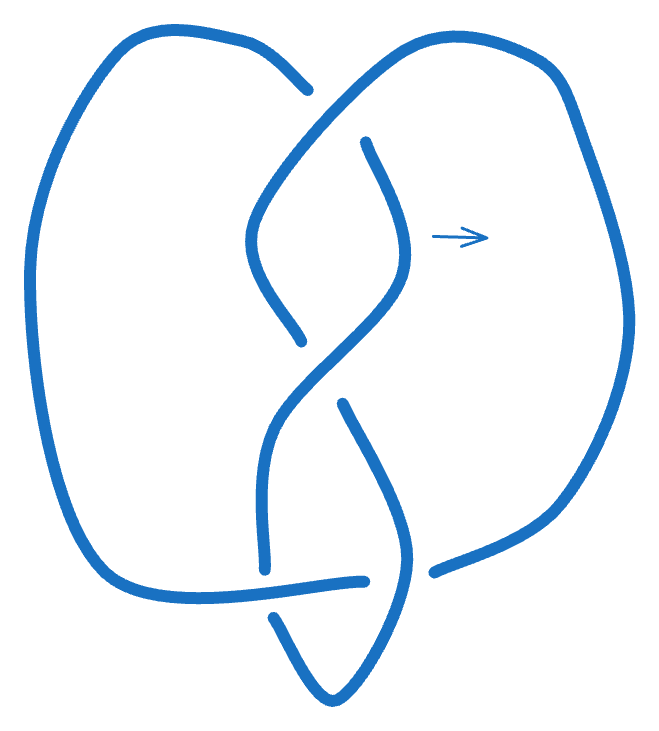
\includegraphics[width=9em]{figs/b2e125_1.png}&
		$\overset{\text{0}}{\sim}$&
		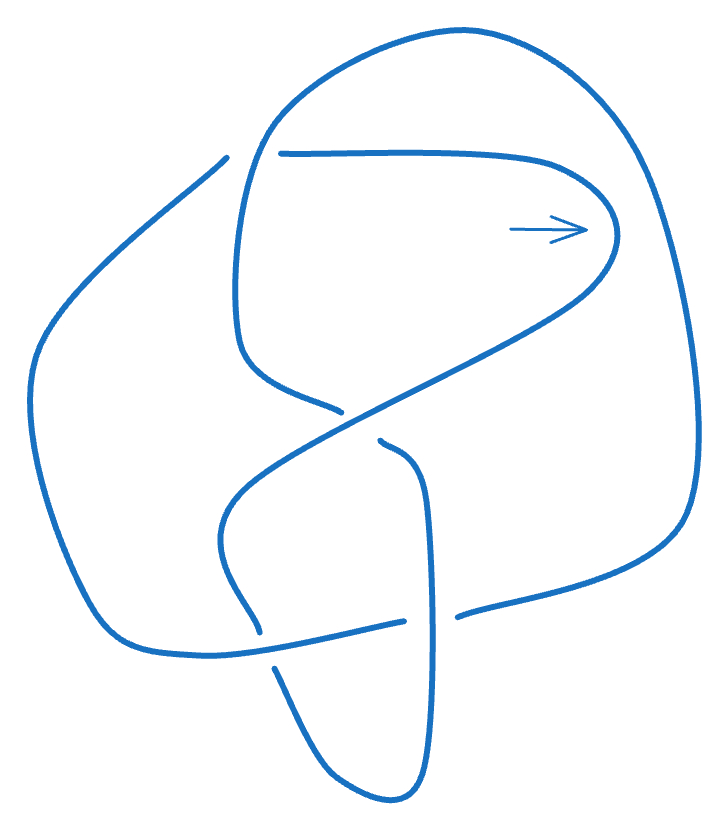
\includegraphics[width=9em]{figs/b2e125_2.png}&
		$\overset{\text{II}}{\sim}$&
		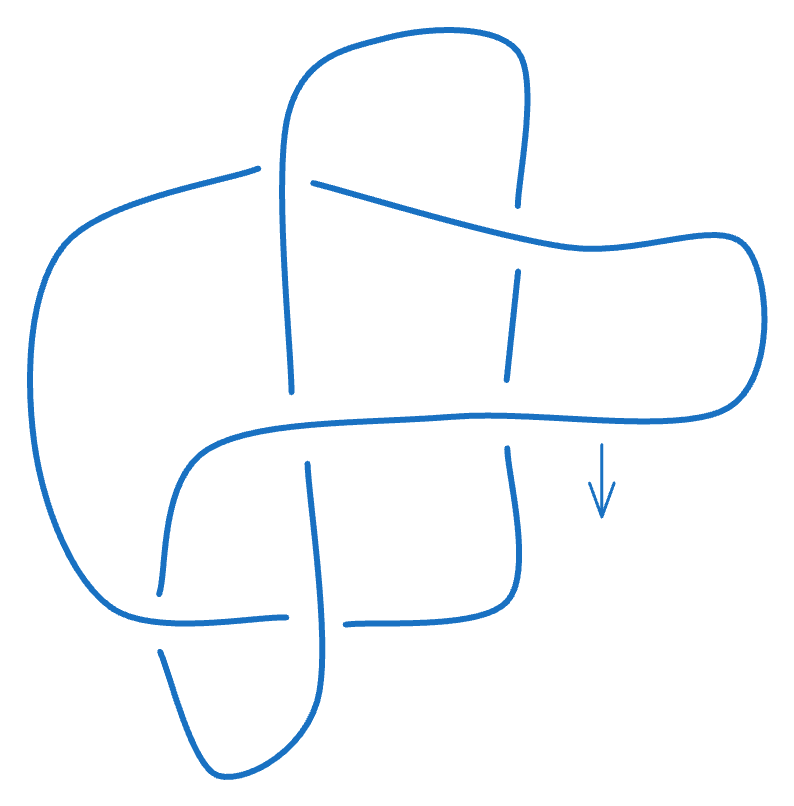
\includegraphics[width=9em]{figs/b2e125_3.png}&
		$\overset{\text{0}}{\sim}$&
		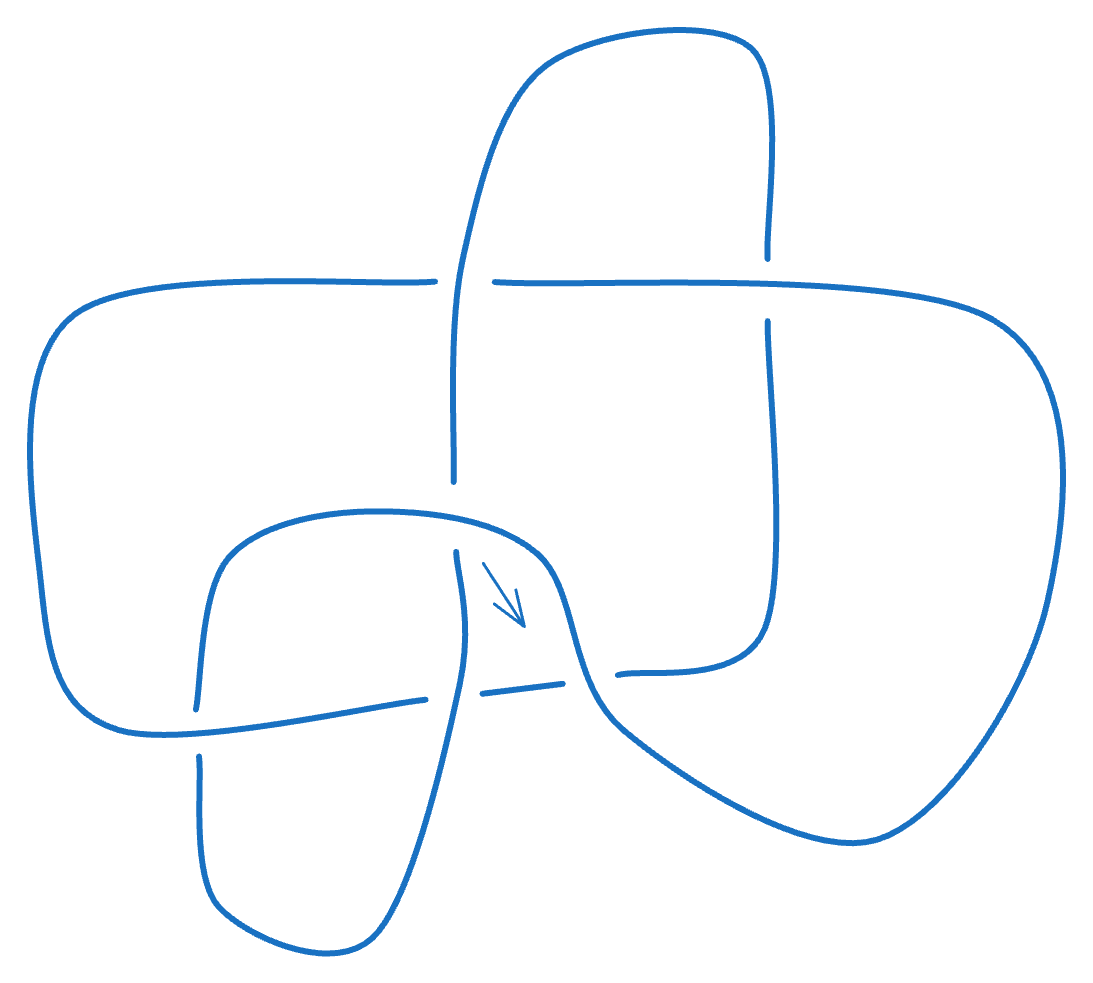
\includegraphics[width=9em]{figs/b2e125_4.png}\\
		&&&&&&\rotatebox[origin=c]{90}{$\sim$}\text{\scriptsize{III}}\\
		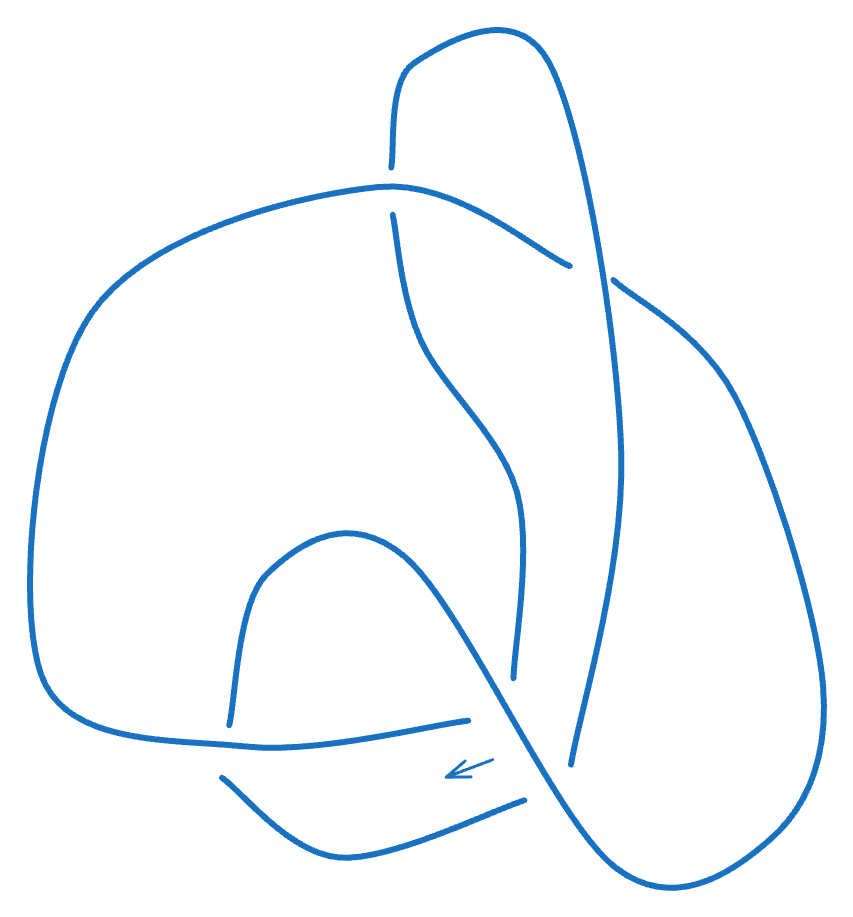
\includegraphics[width=9em]{figs/b2e125_8.png}&
		$\overset{\text{I}}{\sim}$&
		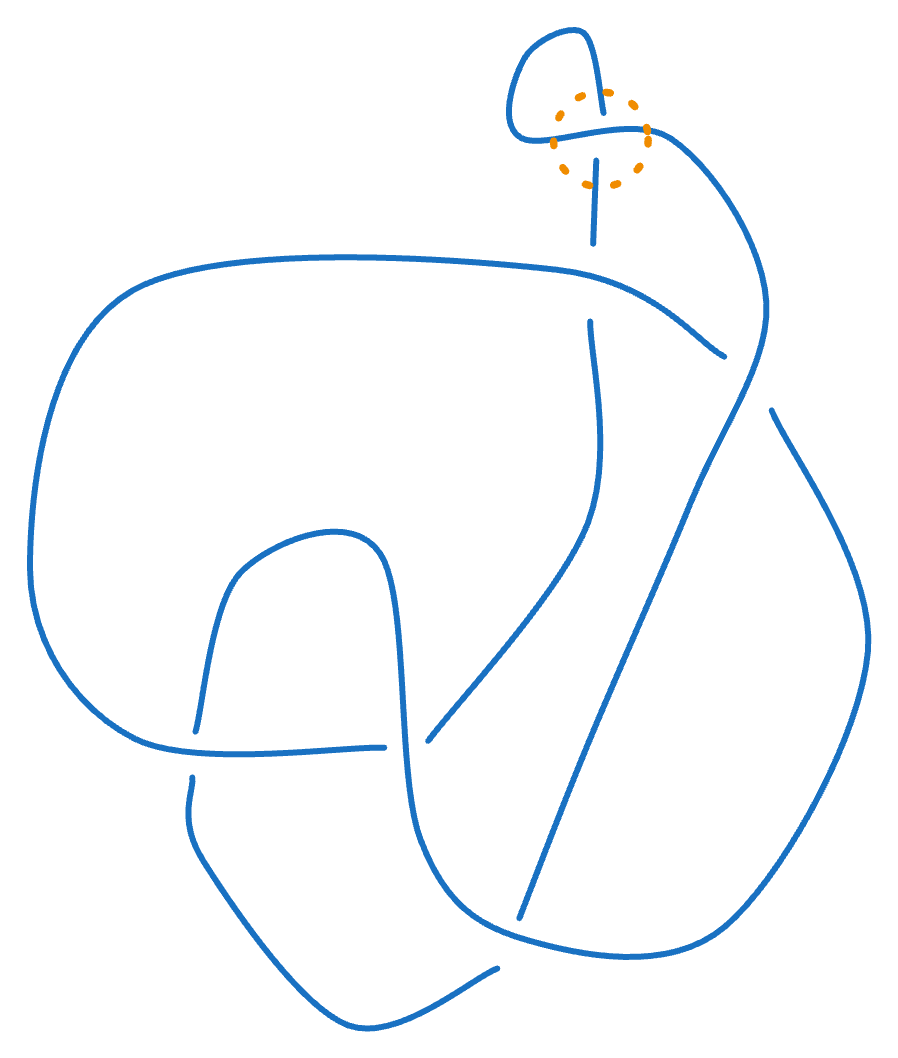
\includegraphics[width=9em]{figs/b2e125_7.png}&
		$\overset{\text{III}}{\sim}$&
		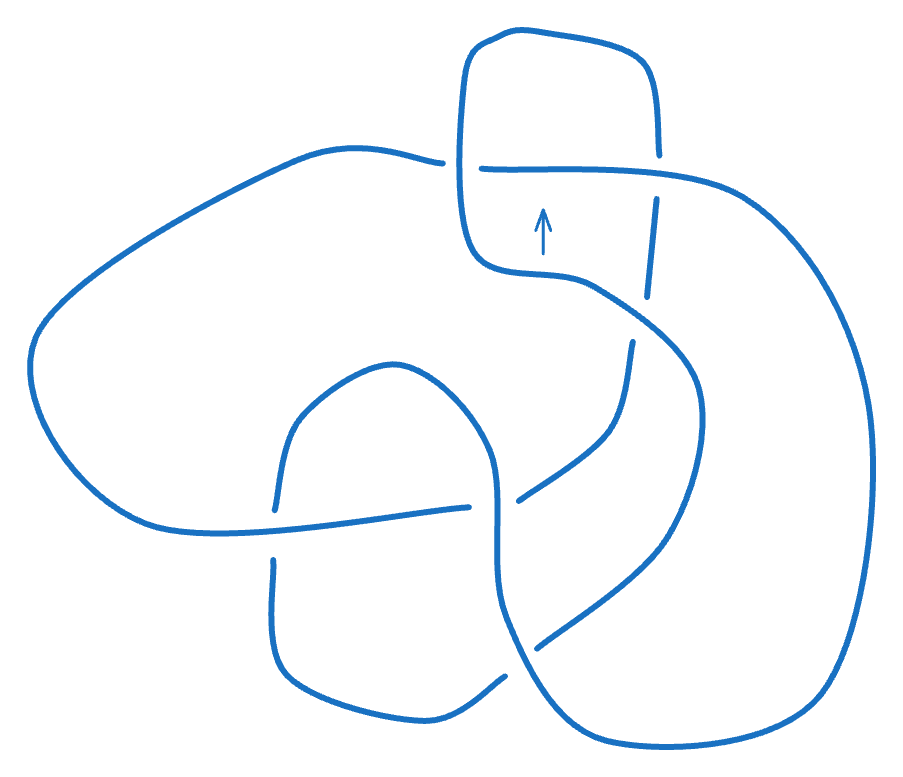
\includegraphics[width=9em]{figs/b2e125_6.png}&
		$\overset{\text{0}}{\sim}$&
		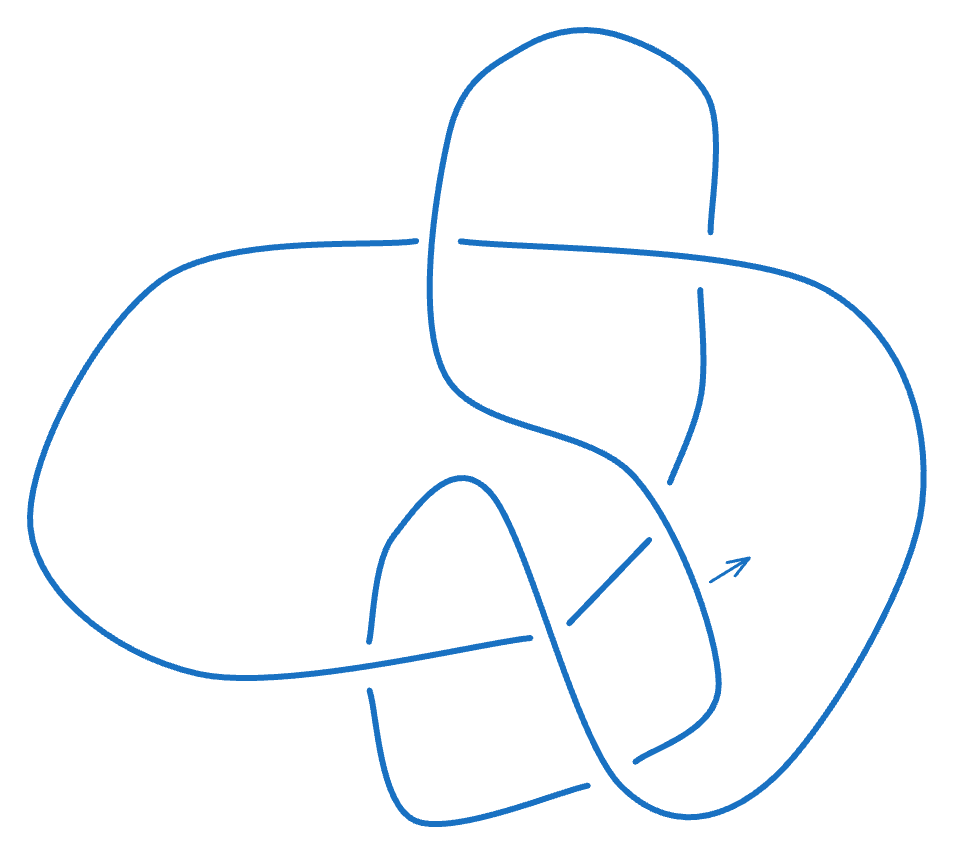
\includegraphics[width=9em]{figs/b2e125_5.png}\\
		\rotatebox[origin=c]{90}{$\sim$}\text{\scriptsize{0}}&&&&&&\\
		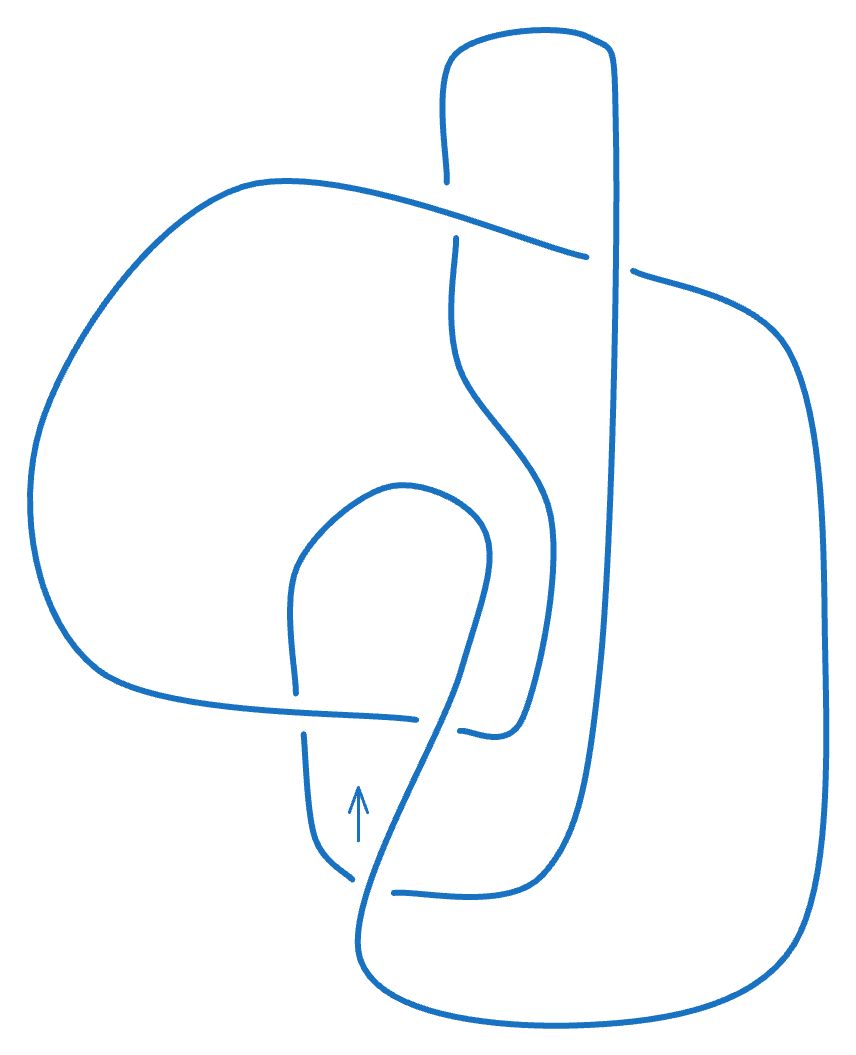
\includegraphics[width=9em]{figs/b2e125_9.png}&
		$\overset{\text{III}}{\sim}$&
		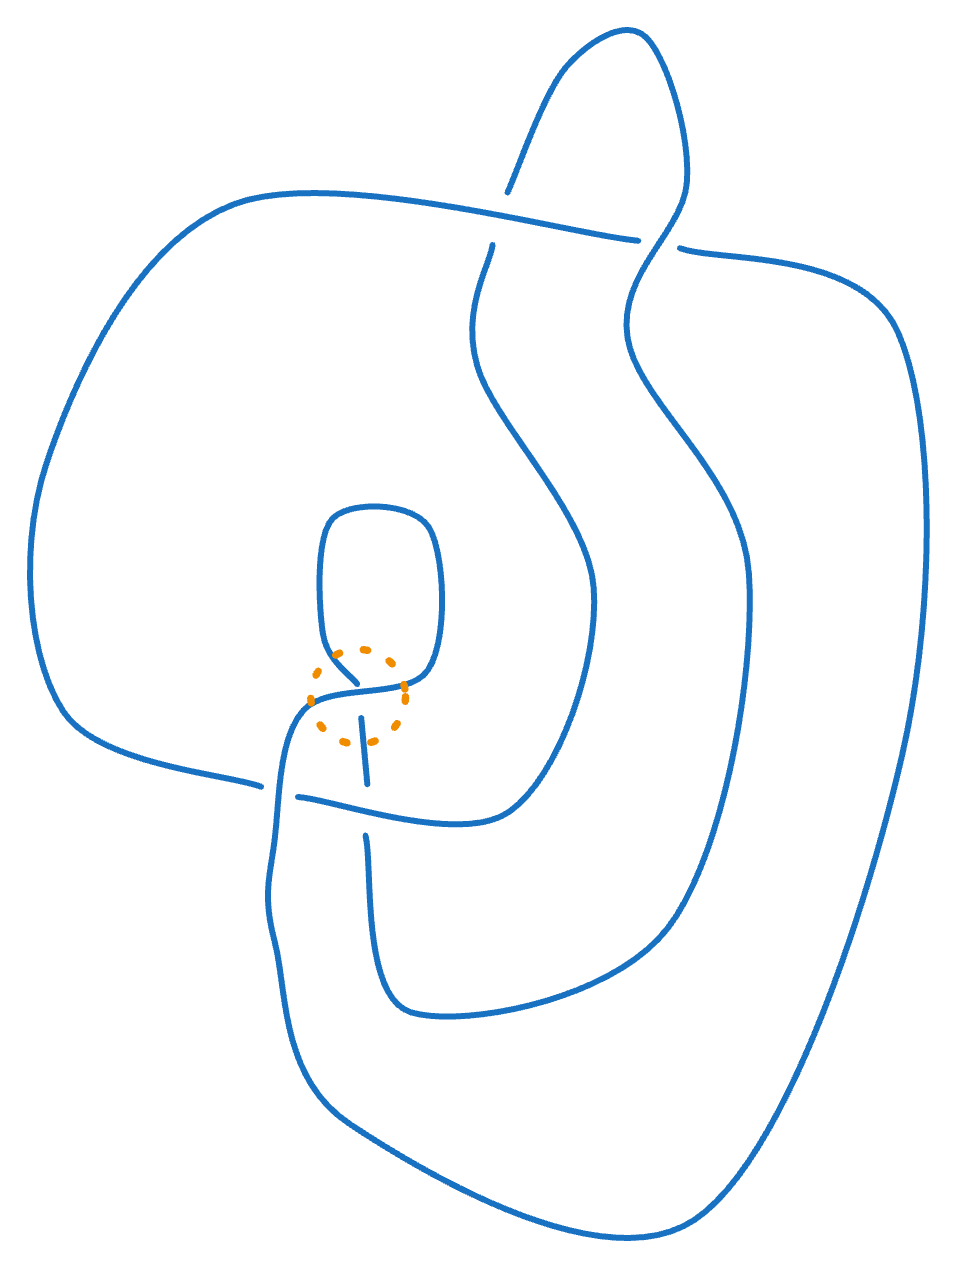
\includegraphics[width=9em]{figs/b2e125_10.png}&
		$\overset{\text{I}}{\sim}$&
		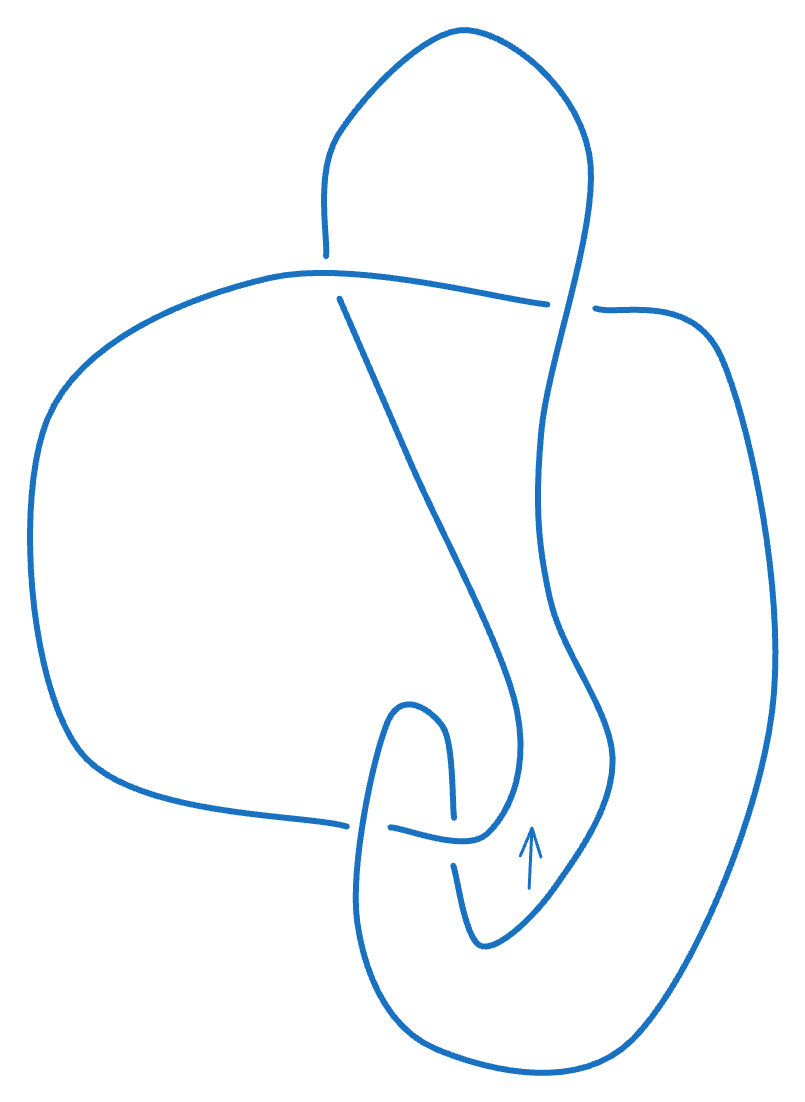
\includegraphics[width=9em]{figs/b2e125_11.png}&
		$\overset{\text{0}}{\sim}$&
		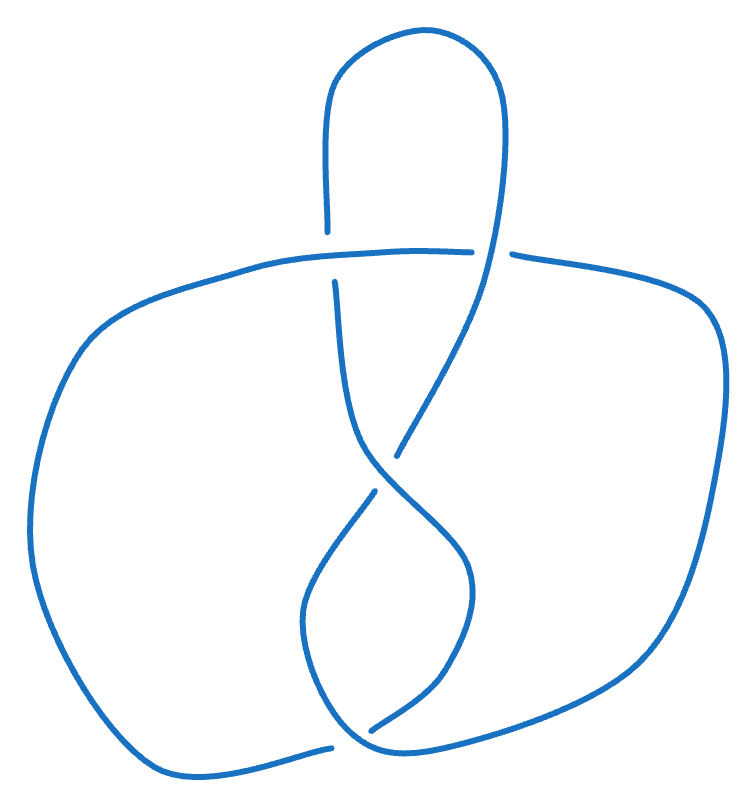
\includegraphics[width=9em]{figs/b2e125_12.png}\\
		&&&&&&\rotatebox[origin=c]{90}{$\sim$}\text{\scriptsize{0}}\\
		&&&&&&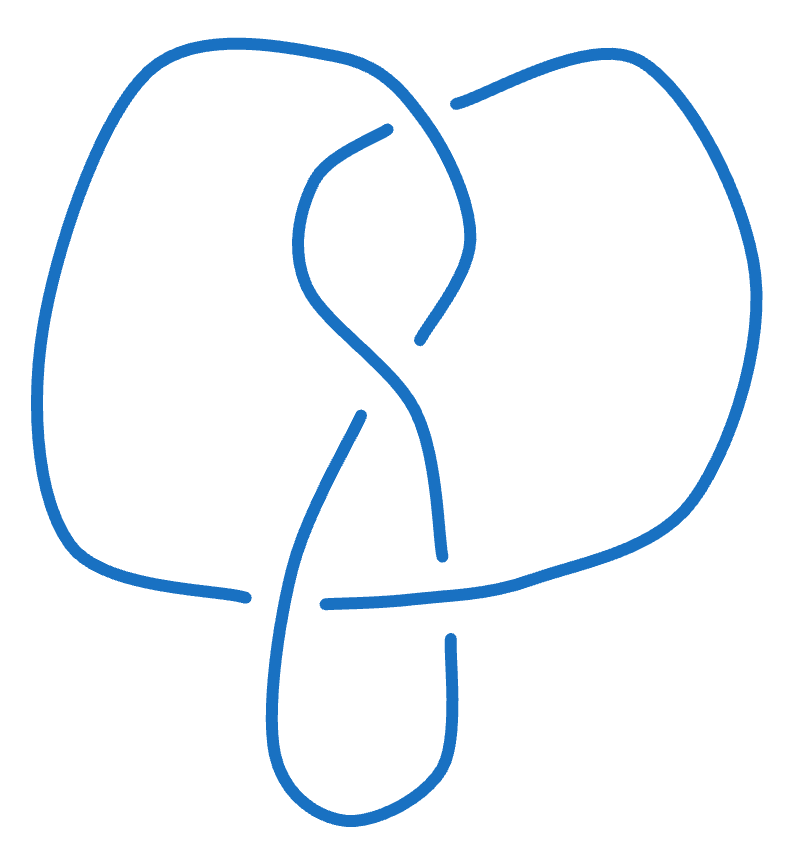
\includegraphics[width=9em]{figs/b2e125_13.png}
	\end{tabular}
\end{center}
The two ends of the sequence are marked by a thicker line. In each step we have an ambient isotopy, denoted by $\sim$.

\begin{example}
	Show using Reidemeister moves that the Perko pair consists of two isotopic knots. (Hint: it might help to make a model with string.)
\end{example}
\sol See {\tt data/perko{\_}gif}, generated from Ref [28].


\begin{example}
	If one allows all possible orientations, there are many oriented versions of the first Reidemeister moves. Find a minimal set of oriented Reidemeister moves from which the rest can be derived.
\end{example}
\sol For each minimal set, we have two orientations $\{\uparrow, \downarrow\}$ per strand. In general for $n$ strands we have $2^n$ oriented Reidemeister moves. So we have for each Reidemeister move:
\begin{enumerate}[label=Move \arabic*:, start=0]
	\item 1 strand $\to 2$ oriented moves
	\item 1 strand $\to 2$ oriented moves
	\item 2 strands $\to 4$ oriented moves
	\item 3 strands $\to 8$ oriented moves
\end{enumerate}


\begin{example}
	Check that the modified first Reidemeister move really gives an isotopy of framed links. (Hint: one can do so either using equations, or using a little piece of ribbon. The latter is definitely more enlightening!)
\end{example}
\sol Using the modified first Reidemeister move on a twisted ribbon, where we no longer have the intermediate step, yet still maintain the same framing:
\begin{center}
	\begin{tabular}{ m{12em} c m{12em}} 
		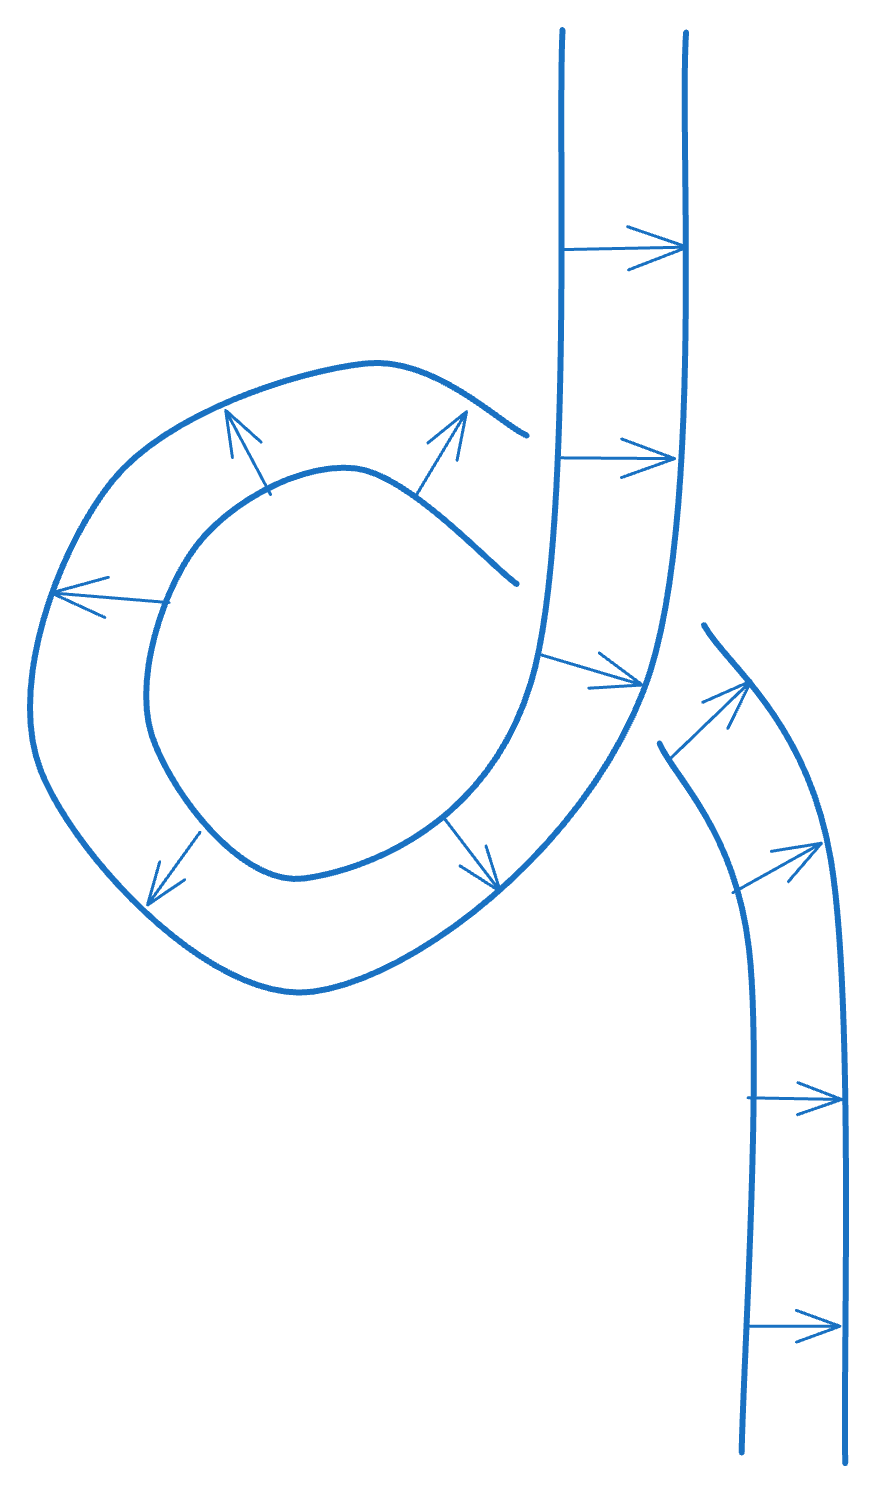
\includegraphics[width=12em]{figs/ribbon_1.png}&
		$\overset{\text{I}^\prime}{\sim}$&
		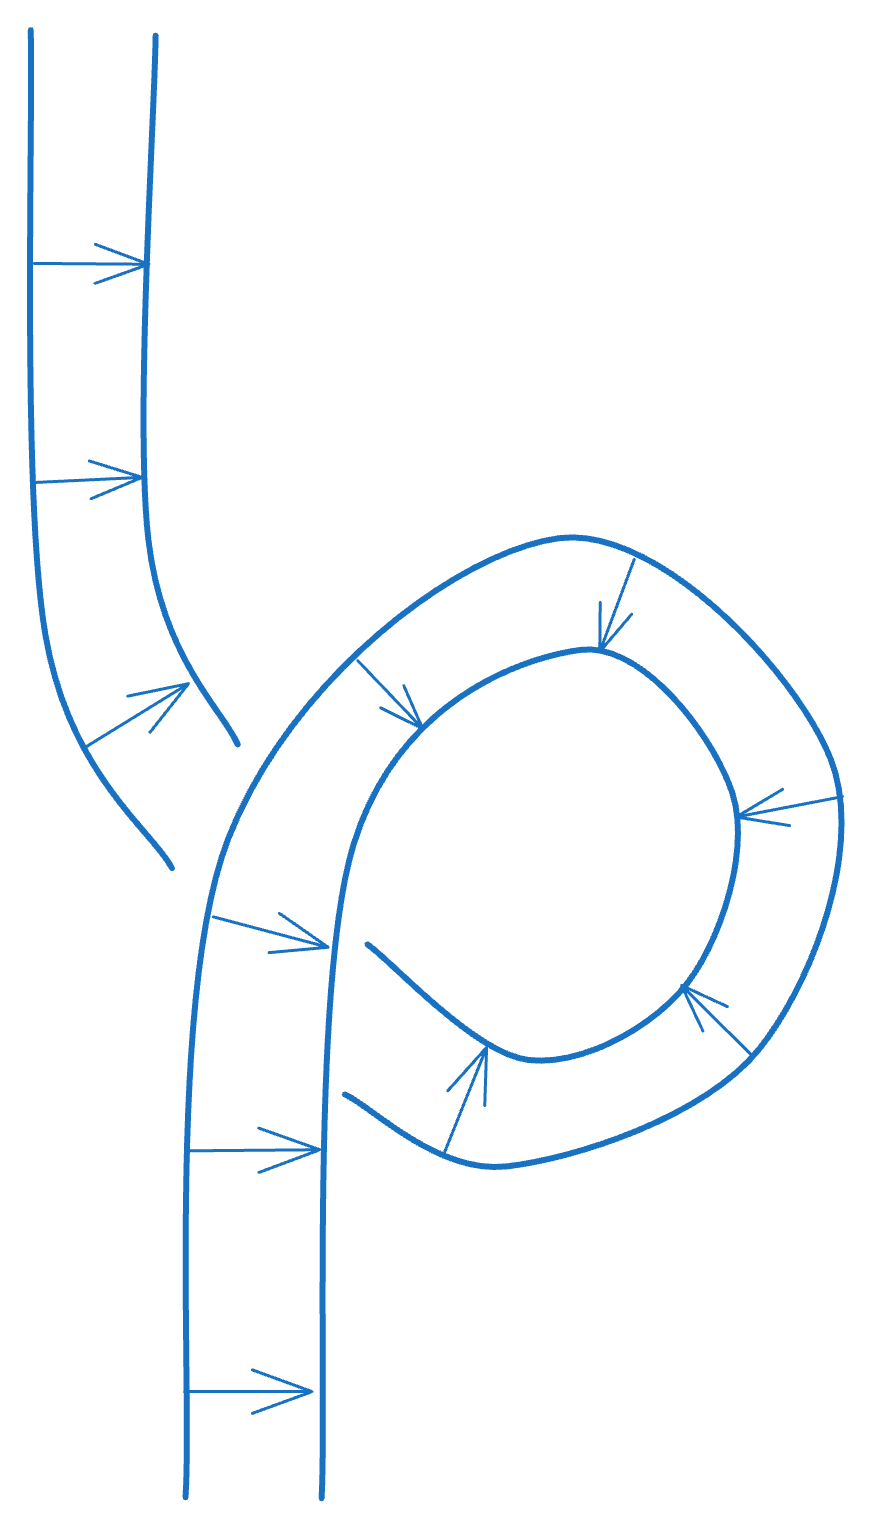
\includegraphics[width=12em]{figs/ribbon_2.png}
	\end{tabular}
\end{center}


\begin{example}\label{b2e129}
	Show using the framed Reidemeister moves that the figure-eight knot and its mirror image in Fig 20 are regular isotopic, hence isotopic as framed knots, giving both the blackboard framing. (Hint: this takes work, and it uses the Whitney trick.)
\end{example}
\sol Note that \emph{opposite twists} happen in these two cases, as we are travelling along the link:
\begin{enumerate}
	\item Like Pg 309, Fig 27 in the text, we have a loop on opposite sides and maintain the same crossing sequence (like ``under'' followed by ``under'').
	\item Or we flip one of the loops, such that they are on the same side, and have an opposite crossing sequence.
\end{enumerate}
Now consider the Type I moves used in Ex \ref{b2e125}. Instead of performing those moves, we leave the twists marked with dotted circles. They form a pair of opposite twists corresponding to Case 2 above. We can then perform a Whitney trick to straighten it out without affecting the framing.\\\\
Thus we claim that the figure-eight knot is regular isotopic to its mirror image.


\begin{example}\label{b2e130}
	Show that the writhe is invariant under Reidemeister moves 0, I$^\prime$, II, and III.
\end{example}
\sol 
Remember that when looking at a complicated link diagram we can rotate a crossing to make sense of it. For example:
\begin{itemize}
	\item \underline{Right-handed}:
	$$
	\mim{figs/rh.png} \sim \mima{figs/rh.png}{90} \sim \mima{figs/rh.png}{180} \sim \mima{figs/rh.png}{270}
	$$
	\item \underline{Left-handed}:
	$$
	\mim{figs/lh.png} \sim \mima{figs/lh.png}{90} \sim \mima{figs/lh.png}{180} \sim \mima{figs/lh.png}{270}
	$$
\end{itemize}
Pg 310 of the text, last paragraph tells us why 0, II, and III preserve linking number and thus writhe. So the only move left to check is I$^\prime$. In this diagram of a twist in a strand of a framed link, we see it preserves number of crossings and handedness:
\begin{center}
	\begin{tabular}{ m{7em} c m{7em}} 
		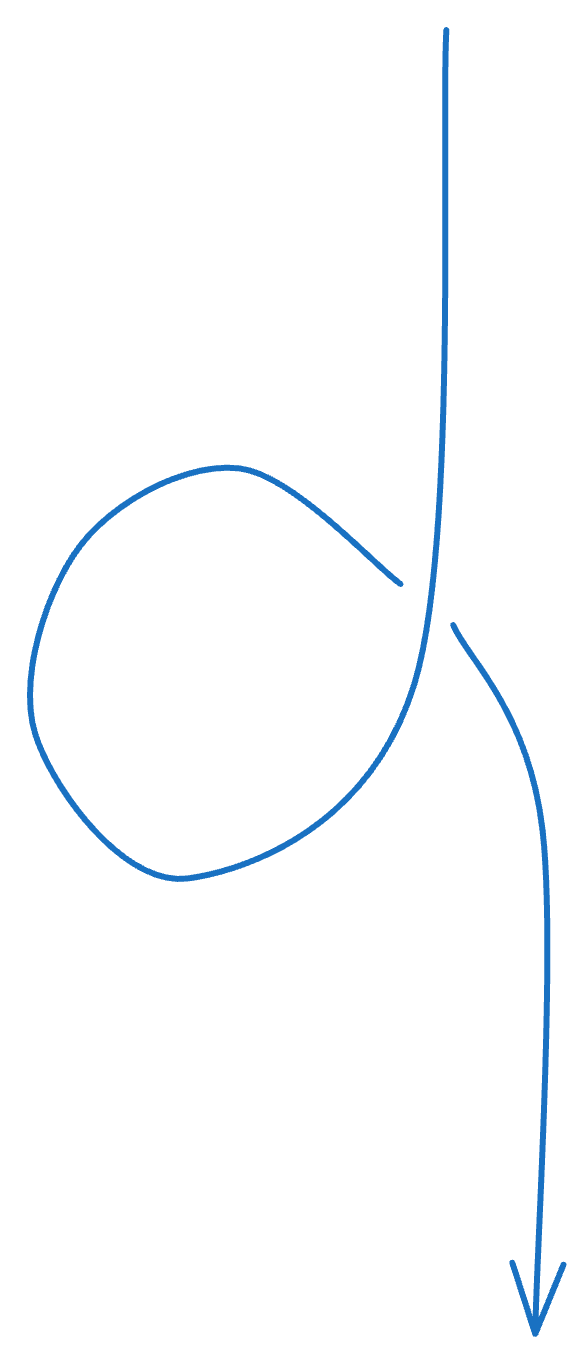
\includegraphics[width=7em]{figs/fl_1.png}&
		$\overset{\text{I}^\prime}{\sim}$&
		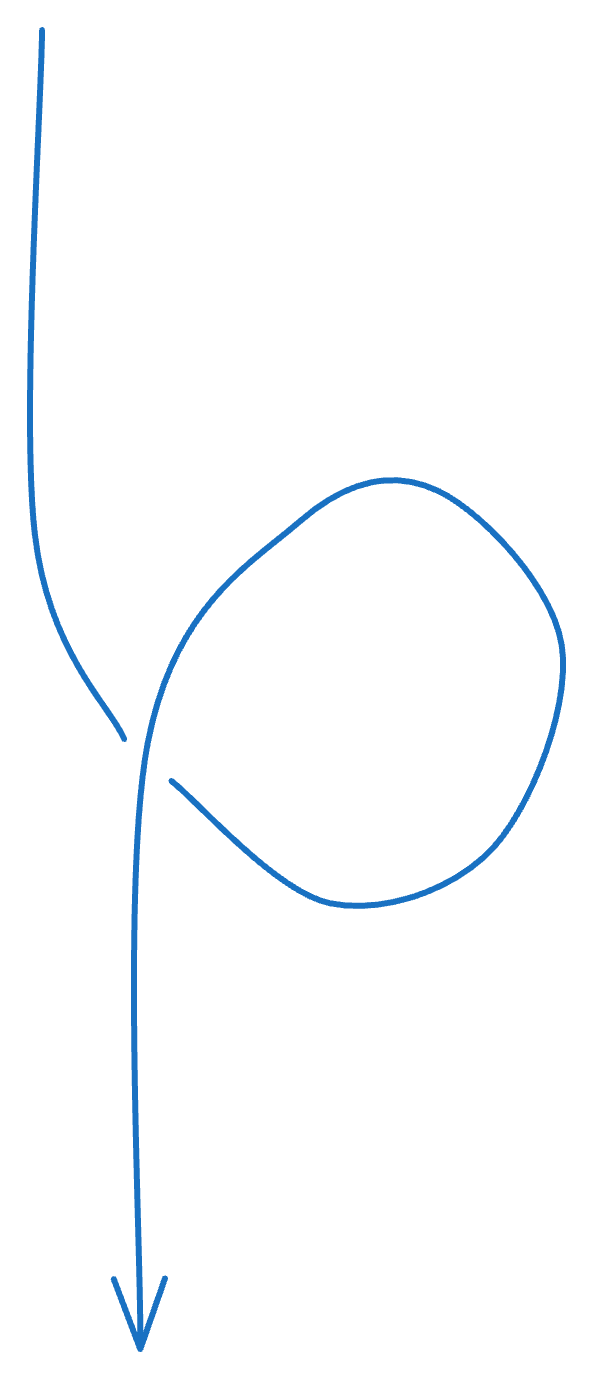
\includegraphics[width=7em]{figs/fl_2.png}
	\end{tabular}
\end{center}
Both these crossings are right-handed. Left-handed crossings (swap ``under'' and ``over'') are preserved as well.


\begin{example}\label{b2e131}
	Show that if $L$ is a link with components $K_i$, then
	$$
	w(L) = \sum_{i\ne j}{\mc L}(K_i,K_j)+\sum_i w(K_i)
	$$
	This is one reason why the writhe is also called the self-linking number.
\end{example}
\sol Writhe - which unlike linking number counts crossings of the same component - is twice the linking number plus number of self-crossings.


\begin{example}
	Deduce the skein relations for the linking number. Note that the first skein relation consists of two cases: the linking number increases by 1 if we change a left-handed crossing to a right-handed crossing when the two strands that cross belong to different components, but does not change when they belong to the same component.
\end{example}
\sol If we have crossings in different components and change from left-handed crossing to right-handed, the sign increases by 2, so the linking number changes by half that. If the crossing is in the same component, like in a twist, it does not matter since the linking number does not track those.


\begin{example}
	By examining the pancake proof, show that $S$ is orientable. Show that if $K^\prime$ is oriented there is a unique orientation on $S$ compatible with the orientation on the $K^\prime$ in the sense explained in Sec \ref{b1c6} - see also Fig 39.
\end{example}
\sol The ``pancake proof'' is also called Seifert's algorithm, details are in Ref [29].
\begin{marginfigure}
	\begin{center}
	  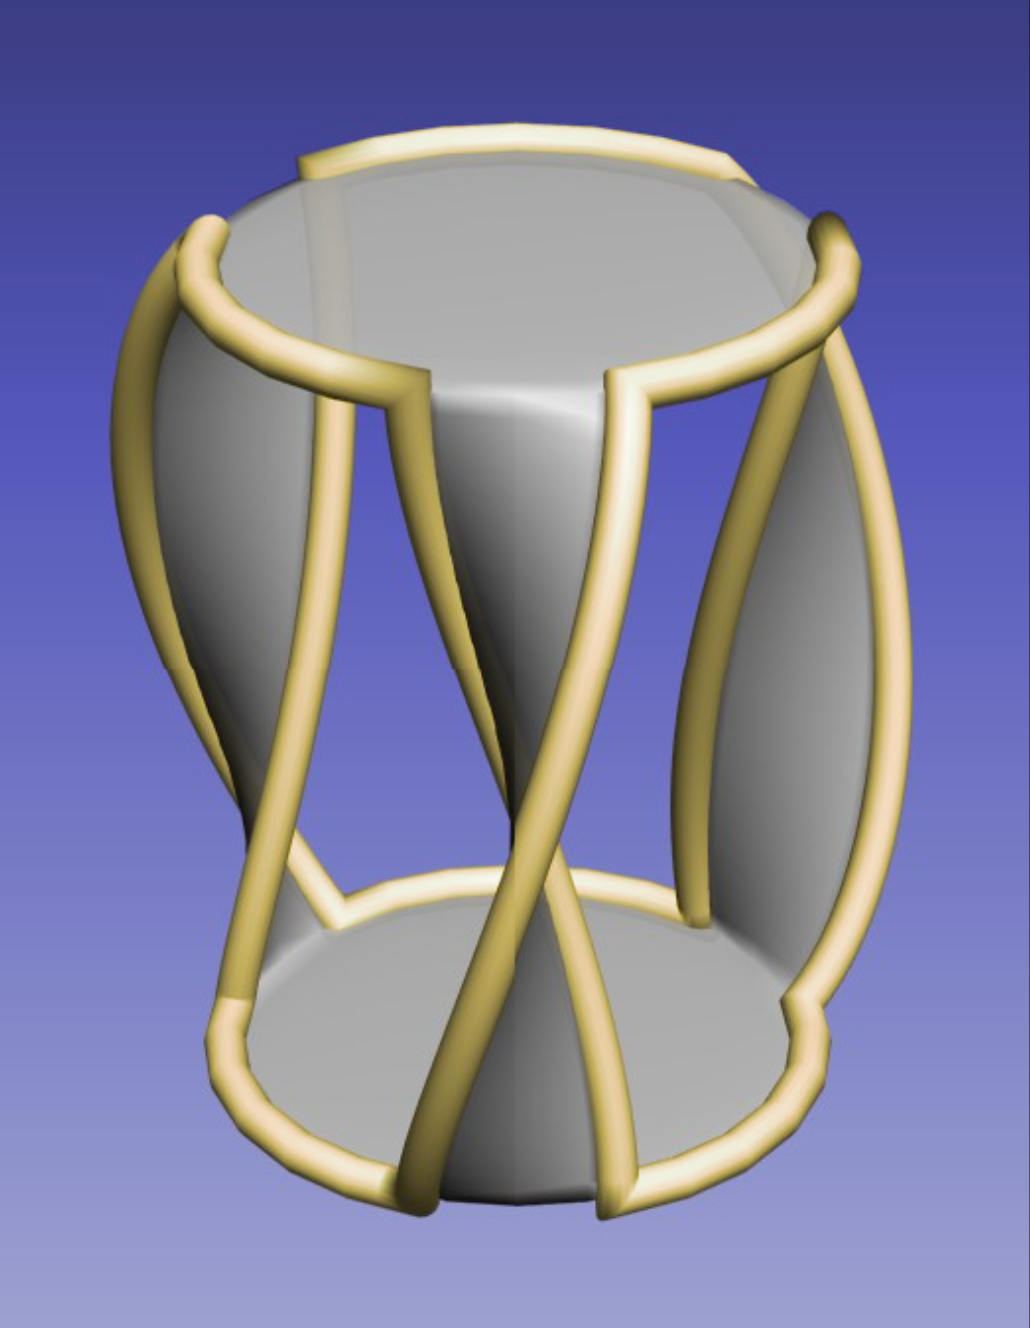
\includegraphics[width=1.2\textwidth]{figs/trefoil_ss.png}
	\end{center}
	\caption{Seifert surface of the trefoil knot (one of many)}
\end{marginfigure}
It is a procedure to construct from a knot $K$ a non-unique, oriented Seifert surface $S$, with $\partial S=K$.\\\\
Each band in $S$ corresponds to a crossing, and has one twist, with orientation derived from the crossing type on the knot. So even though the Seifert surface can be represented in many ways, the orientation depends on that chosen for the knot.


\begin{definition}
	Let $K, L \subseteq M$ be s.t. $\dim K + \dim L = \dim M$. $K$ and $L$ are \tb{transversal} in $M$, written as $K \pitchfork_M L$ if:
	\begin{itemize}
		\item $K$ and $L$ generically intersect in discrete points
		\item At all these intersection points $K$ and $L$ are not tangent (i.e they make non zero angles)
	\end{itemize}
	Transversality is a robust condition because:\marginnote{See Ref [30]}
	\begin{itemize}
		\item $K \pitchfork_M L \implies$ small perturbations keep transversality
		\item $K \not\pitchfork_M L \implies$ small perturbations create transversality
	\end{itemize}
\end{definition}


\begin{example}
	Check them.\mn{Skein relations for the intersection number of $K$ and $S$, where $S$ is the Seifert surface of $K^\prime$}
\end{example}
\sol TODO
% Skein relations for the intersection number:
% \begin{itemize}
% 	\item When $K,K^\prime$ are in different components (same as Fig 41 in the text)
% 	\item When $K,K^\prime$ are in same component
% \end{itemize}


\begin{example}
	Check that this integral does not depend on which vector potential $A$ we choose such that $dA=B$.
\end{example}
\sol Assuming $dA=B$, we can choose any vector potential $A^\prime$ up to a gauge transformation which means $A,A^\prime$ are in the same cohomology class. So they differ by an exact form (say $dC$), such that $A^\prime-A=dC$. So
$$
\begin{aligned}
	A^\prime&=A+dC\\
	\Rightarrow \int_{\R^3}A^\prime\wedge B &= \int_{\R^3}A\wedge B + \int_{\R^3}dC\wedge B\\
	&=\int_{\R^3}A\wedge B + \int_{\partial\R^3}C\wedge B{\:\color{red}+}\int_{\R^3}C\wedge dB\marginnote{See Ref [1]}\\
	&=\int_{\R^3}A\wedge B + \cancel{\int_{\partial\R^3}C\wedge B}{\:\color{red}+}\cancel{\int_{\R^3}C\wedge d(dA)}\marginnote{$B=dA$ and $\partial\R^3=\emptyset$ because $\R$ is both open and closed}\\
	&= \int_{\R^3}A\wedge B
\end{aligned}
$$
\underline{Pedagogical note:}\\\\
The {\color{red}+} marked with a color is different compared to what we see in Ref [1] Pg 169 (integration by parts on wedge product, with 0-form $f$). This is to show the Leibniz rule applied here where $C$ is a 1-form. But it doesn't matter because this quantity vanishes.


\begin{example}
	Check this computation.\mn{Pg 326 of the text}
\end{example}
\sol Using Ex \ref{b2e131} justifies the formula on Pg 325:
$$
w(K)={\mc L}(K_\alpha,K_\beta)
$$
% \begin{marginfigure}
% 	\begin{center}
% 		\vspace{15em}
% 	  	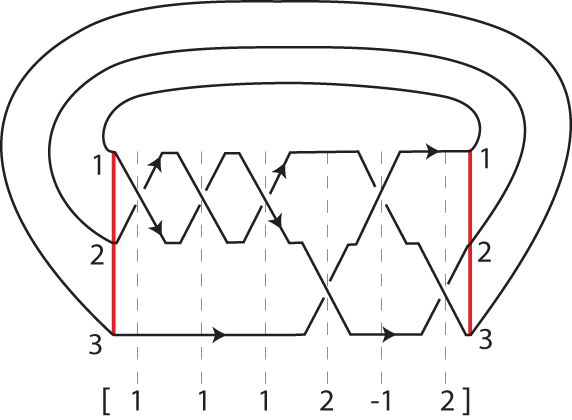
\includegraphics[width=1.2\textwidth]{figs/braid.png}
% 	\end{center}
% 	\caption{A braid representation of the knot $5_2$}
% \end{marginfigure}
% \begin{marginfigure}
% 	\begin{center}
% 		\vspace{15em}
% 	  	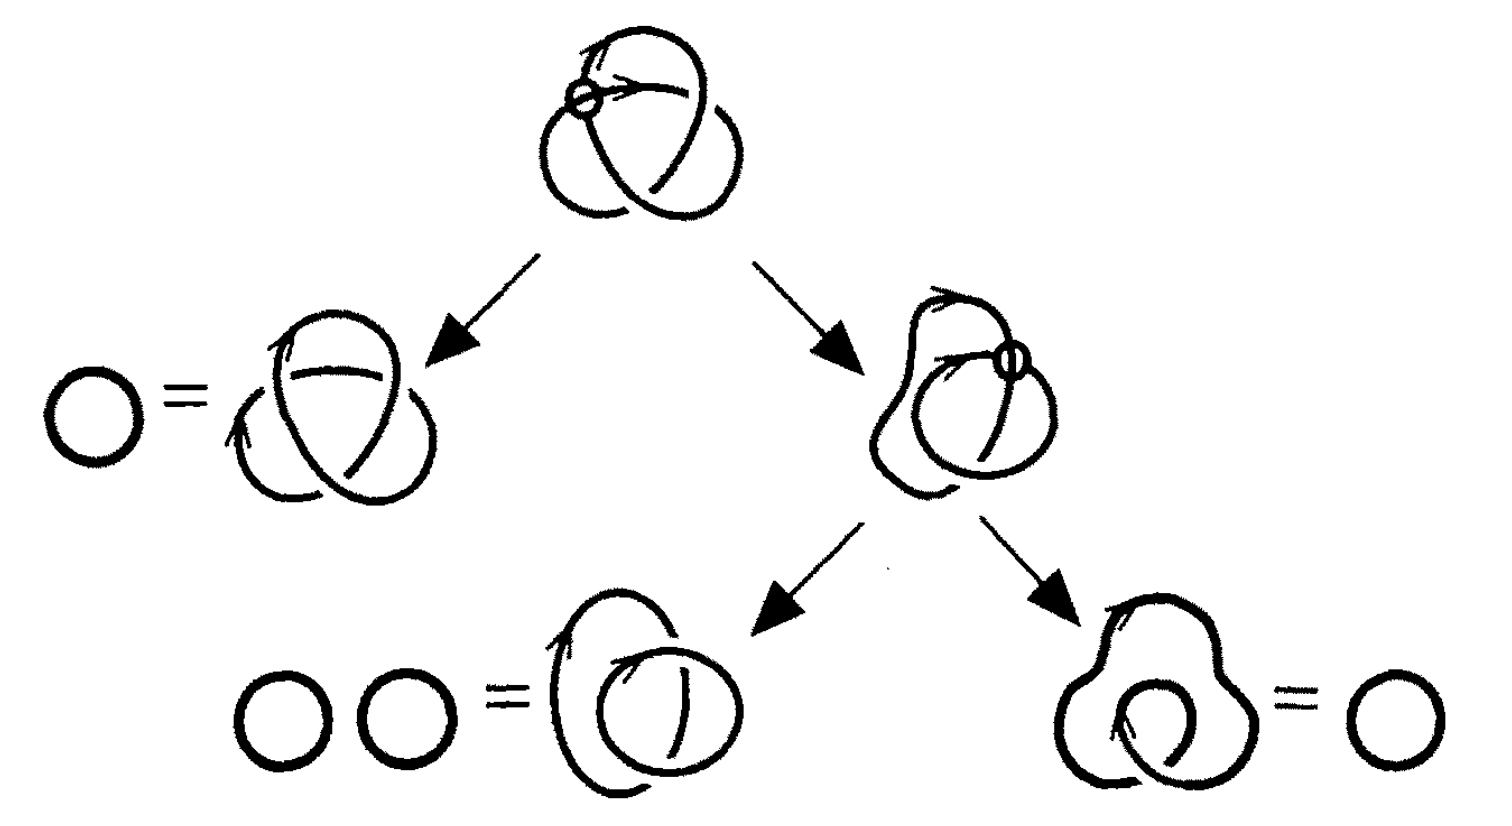
\includegraphics[width=1.2\textwidth]{figs/trefoil_tree.png}
% 	\end{center}
% 	\caption{Resolving tree for the trefoil knot}
% \end{marginfigure}


\begin{example}
	Write\mn{We slightly modify the notation to follow the argument in Theorem 6.1.5 of Ref [33]}
	$$
	\nabla_L(z)=\sum_{i=0}^{\infty}a_i(L)z^i.
	$$
	Show that $a_0$ is 1 if $L$ has exactly one component, and 0 otherwise. Show that $a_1$ is the linking number of $L$ if $L$ has exactly two components, and 0 otherwise.
\end{example}
\sol We can rewrite the skein relations in Fig 44 of the text in a more algebraic way:
\begin{itemize}
	\item $\nabla(0_1) = 1$ where $0_1$ is the unknot.
	\item $\nabla_{L_+} - \nabla_{L_-} = z\nabla_{L_0}$.
	\item If $L$ is split, $\nabla_L(z) =0$.
\end{itemize}
Let the link $L$ have $c$ components and $n+1$ crossings. We can write:
$$
\nabla_L(z)=\nabla_{L^\prime}(z)+z\nabla_{L_1}(z)+\cdots+z\nabla_{L+m}(z)
$$
where the $L_i$ are a sequence of links with $c-1$ components and $n$ crossings. The link $L^\prime$ is an unlink obtained after uncrossing $m$ crossings.\\\\
Observe that $a_0(L)=\nabla_L(0)$. Evaluating the skein relation at 0 shows that changing any crossing of $L$ doesn't modify $a_0(L)$. By unknotting, we obtain $a_0(L)=1$.\\\\
Suppose $L$ has components $L_1$ and $L_2$ with $\mc{L}(L_1,L_2)=n$. Assume wlog. that $n \ge 0$. Consider the skein relation with $L_+=L$, and change one of the crossings of the two components. Then $L_-$ has two components $L_1^\prime$ and $L_2^\prime$, and $L_0$ has one component. Then
$$
\mc{L}(L_1,L_2)-\mc{L}(L_1^\prime,L_2^\prime) = 1 = a_0(L_0) = a_1(L_1) - a_1(L_-).
$$
By induction, the linking number $\mc{L}(L_1, L_2)$ is equal to $a_1(L)-a_1(\tilde{L})$. where $\tilde{L}$ is a link
with two components with crossing number 0. In particular, we could have chosen $\tilde{L}$ to be a split link, so $\mc{L}(L_1, L_2) = a_1(L)$.
% If $L$ has exactly one component, when we go through the process of undoing all the crossings we will always end up with an unknot. According to skein relations in Fig 44 of the text, the unknot has $\nabla_L(z)= 1$, in other words the Alexander polynomial for $L$ is just the constant term $a_0=1$.\\\\
% % To calculate $\nabla_L(z)$ for more components we can repeatedly choosing a crossing, and then apply the skein relations in Fig 44\marginnote{Ref [31], Pg 167} to obtain two simpler links, which yields a tree of links called the \emph{resolving tree}. 
% The skein relations are quite fiddly, so here is another way of calculating the Alexander polynomial\marginnote{Ref [31] Pg 129, Ref [32]}. Alexanders theorem states that every link can be represented by a closed braid. Such a representation determines a Seifert surface $S$ for the link. Given $S$ and a basis of the first homology group\mn{The first homology group, $H_1(X)$, is the abelianization of the fundamental group, $\pi_1(X)$. Abelian groups have a well-defined structure theorem, which states that any finitely generated abelian group can be decomposed into a direct sum of cyclic groups. The generators of these cyclic groups can be considered a basis for the abelian group.} of $S$, we can generate a Seifert matrix $M$ which has the property:
% $$
% \nabla_L(z)=\det(M-zM^\intercal)
% $$
% % In the case of two components, $M$ is simply a 1x1 matrix with the linking number of . For example in the Hopf link it would be $\pm1$. So we get $\nabla_{\text{Hopf}}(z) = \pm(1-z)$. In general $\nabla_L(z) = \pm(1-z)$
% For a general link $L$ with two components\marginnote{TODO find out why}
% $$
% M = \begin{pmatrix}
% 	a&b\\c&d
% \end{pmatrix}
% $$
% where
% \begin{itemize}
% 	\item $a$ is the self-linking number of the first component
% 	\item $d$ is the self-linking number of the second component
% 	\item $b,c$ are the linking numbers between the two components
% \end{itemize}
% So
% $$\begin{aligned}
% 	\nabla_L(z)&=\det(\begin{pmatrix}
% 		a&b\\c&d
% 	\end{pmatrix}-z\begin{pmatrix}
% 		a&c\\b&d
% 	\end{pmatrix})\\
% 	&=\ub{-b c + a d}{a_0}+ \ub{(b^2 + c^2 - 2 a d)}{a_1} z + \ub{(-b c + a d)}{a_2} z^2
% \end{aligned}$$
% where $a_1 = b^2 + c^2 - 2 a d$



\begin{example}
	Given an oriented link $L$, let $L^*$ denote its mirror image. Show that $\nabla_L(z)=\nabla_{L^*}(z)$. Thus the Alexander polynomial is unable to distinguish between links and their mirror images.
\end{example}
\sol Turning an oriented link $L$ into $L^*$ involves swapping left and right-handed crossings, as well as reversing the overall orientation. 
\begin{center}
	\begin{tabular}{ c | c} 
		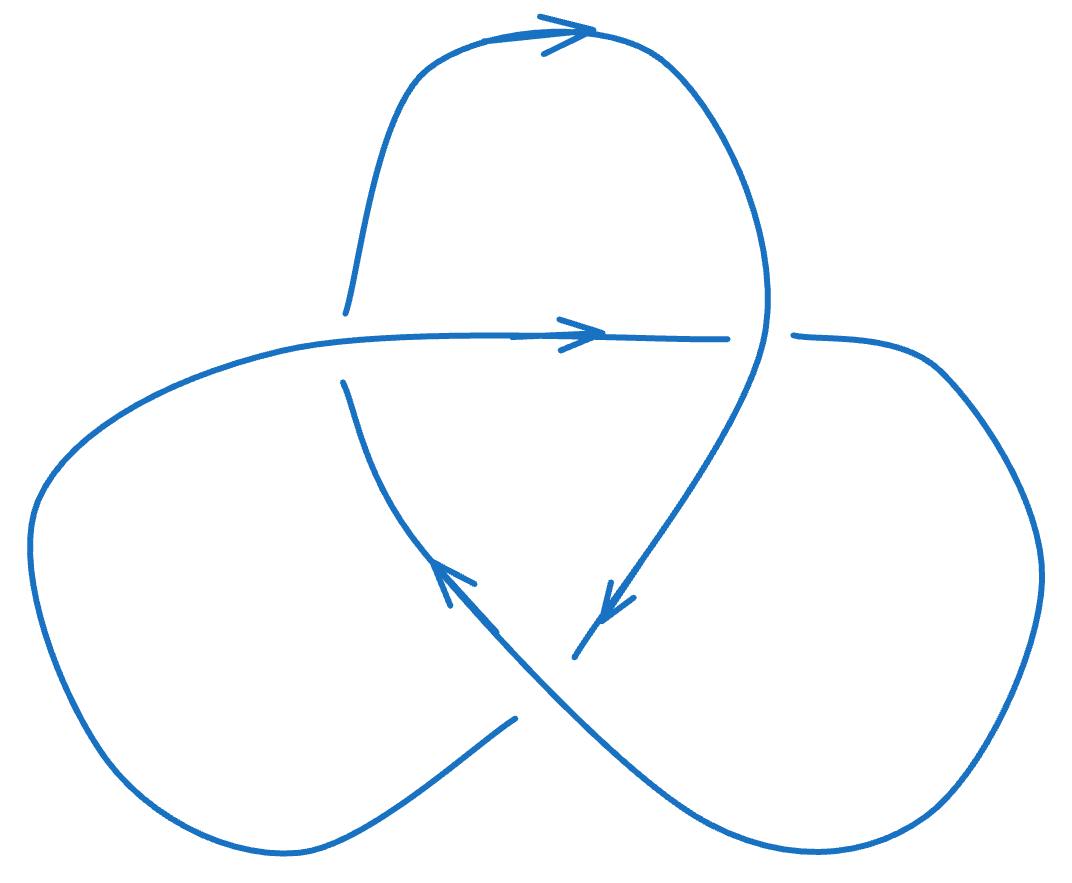
\includegraphics[width=9em]{figs/b2e138_1.png}&
		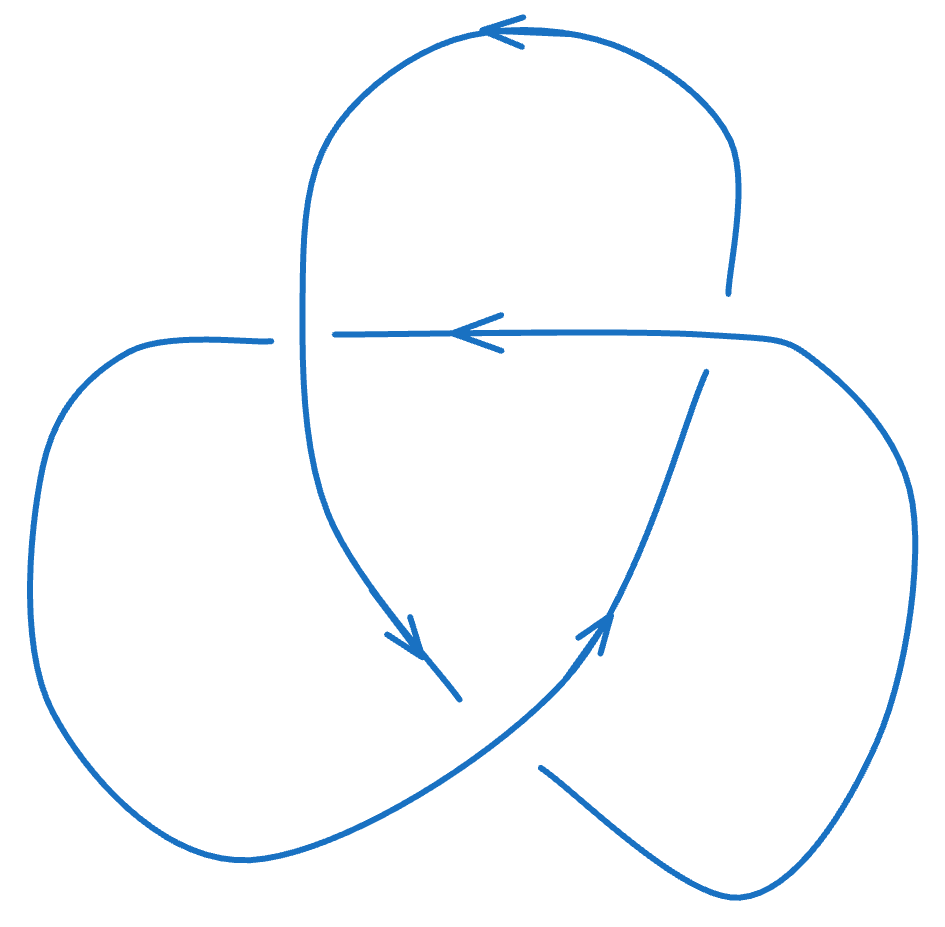
\includegraphics[width=9em]{figs/b2e138_2.png}\\
		$L$&$L^*$
	\end{tabular}
\end{center}
Reading off the handedness from Ex \ref{b2e130}, this does not change the Alexander polynomial because the skein relations stay the same:
$$
\begin{aligned}
	\ub{z\:\:\mims{figs/dd.png}{2em} = \mim{figs/rh.png} - \mim{figs/rh.png}}{\text{Skein relation for }\mc L} &= \ub{\mima{figs/lh.png}{180} - \mima{figs/rh.png}{180} = z\:\:\mims{figs/uu.png}{2em}}{\text{Skein relation for }\mc L^*}\\
	\ub{1 = \mim{figs/circ_l.png}}{\text{Skein relation for }\mc L} &= \ub{\mim{figs/circ_r.png} = 1}{\text{Skein relation for }\mc L^*}
\end{aligned}
$$


\begin{example}
	Check that this process\mn{Eliminating crossings according to whether $\sigma_p$ is $A$ or $B$} is really well-defined, that is, there is no ambiguity about what to do!
\end{example}
\sol From Ex \ref{b2e130}, we see that without orientation (arrows), we can always switch ``under'' to ``over'' and vice versa by just doing a $90^\circ$ rotation, thereby getting it to look like Fig 46 in the text. Doing the $\sigma_p$ assignments per crossing is unambiguous also.


\begin{example}
	Show that
	$$
	-\frac{d}{d\beta}\ln Z(\beta) = \frac{1}{Z(\beta)} \sum_{\text{states }s}E(s)e^{-\beta E(s)}.
	$$
	This is the expected value of the energy of the system at temperature $T$, usually written $\overline E$.
\end{example}
\sol $$
\begin{aligned}
	\overline E &= -\frac{d}{d\beta}\ln Z(\beta)\\
	&= -\frac{1}{Z(\beta)}\frac{d}{d\beta}Z(\beta)\\
	&= -\frac{1}{Z(\beta)}\frac{d}{d\beta}\p*{\sum_{\text{states }s}e^{-\beta E(s)}}\\
	&=\frac{1}{Z(\beta)} \sum_{\text{states }s}E(s)e^{-\beta E(s)}
\end{aligned}
$$


\begin{example}
	Show that
	$$
	\frac{d\overline{E}}{dT} = k\beta^2\frac{d^2}{d\beta^2}\ln Z(\beta).
	$$
	This quantity, which measures the change in expected energy with change in temperature, is called the \tb{specific heat} of the system at temperature $T$.
\end{example}
\sol Since $\beta=1/kT$:
$$
	d\beta=d\p*{\frac{1}{kT}}=\frac{1}{k}\frac{-1}{T^2}dT=-k\beta^2dT
$$
So
$$
\begin{aligned}
	\frac{d\overline E}{dT} &= \frac{d}{dT}\p*{-\frac{d}{d\beta}\ln Z(\beta)}\\
	&= k\beta^2\frac{d^2}{d\beta^2}\ln Z(\beta)
\end{aligned}
$$


\begin{example}\label{b2e142}
	Show that one can get rid of a left-handed twist in the framing while multiplying by $-A^{-3}$. (Hint: one can do this directly or by reducing it to the right-handed case via the Whitney trick.)
\end{example}
\sol Inspired by Fig 51 in the text, for a left-handed twist we have
$$
\begin{aligned}
	\bk*{\mims{figs/twist_l.png}{4em}} &= A\bk*{\mims{figs/bulge_l.png}{3em}} + B\bk*{\mims{figs/line_loop_1.png}{4em}}\\
	&= A\bk*{\mims{figs/line.png}{0.3em}} + Bd\bk*{\mims{figs/line.png}{0.3em}}\\
	&= (A+Bd)\bk*{\mims{figs/line.png}{0.3em}}
\end{aligned}
$$
where 
$$
A+Bd =A-A^{-1}(A^2+A^{-2})= \cancel{A-A}-A^{-3}= -A^{-3}
$$
which is different from the $-A^3$ factor for getting rid of the right-handed twist.


\begin{example}\label{b2e143}
	Show that the Kauffman bracket of the trefoil knot shown in Fig 3 equals $-(A^2+A^{-2})(-A^5-A^{-3}+A^{-7})$. Show that the Kauffman bracket of the unknot (with an arbitrary choice of framing) is $-(A^2+A^{-2})(-A^3)^w$, $w$ being the writhe. Conclude that the trefoil is not isotopic to the unknot, i.e., the trefoil knot is really knotted!
\end{example}
\sol From Ex \ref{b2e142} we get that for an arbitrarily twisted unknot
$$
\begin{aligned}
	&\bk*{\mims{figs/unknot_twisted.png}{50em}}\\
	&=[(-A^{-3})(-A^{-3})(-A^3)(-A^3)\cdots]\bk*{\mim{figs/circ.png}}\marginnote{Undo all twists}\\
	&=[(-A^{-3})(-A^{-3})(-A^3)(-A^3)\cdots]d\\
	&=-(A^2+A^{-2})[(-A^3)^w]
\end{aligned}
$$
where each left/right-handed twist contributes a factor of $-A^{-3}/-A^3$ respectively, which is correctly accounted for by the writhe $w$.\\\\
Now for the trefoil:
$$
\begin{aligned}
	\bk*{\mims{figs/b2e143_1.png}{9em}} &= A\bk*{\ub{\mims{figs/b2e143_2.png}{9em}}{\text{Hopf link}}}+A^{-1}\bk*{\ub{\mims{figs/b2e143_3.png}{9em}}{\text{Unknot with writhe -2}}}\\
	&=A[(A^2 + B^2) d^2 + 2 A B d] + A^{-1} [d (-A^3)^{-2}]\marginnote{Fig 50 in the text, and $w=-2$ for two left-handed crossings}\\
	&= -(A^2+A^{-2})(-A^5-A^{-3}+A^{-7})
\end{aligned}
$$


\begin{example}\label{b2e144}
	Calculate the Kauffman bracket of the mirror image of the previous trefoil knot. Conclude that the trefoil is not isotopic to its mirror image.
\end{example}
\sol Using a procedure similar to Ex \ref{b2e143}, we get:
$$
\bk*{\mims{figs/b2e144_2.png}{9em}} = -(A^2+A^{-2})(-A^7-A^{3}+A^{-5}) \ne \bk*{\mims{figs/b2e144_1.png}{9em}}
$$


\begin{example}\label{b2e145}
	Show that for any framed link $L$, the mirror image $L^*$ has
	$$
	\bk{L^*}(A)=\bk{L}(A^{-1}).
	$$
\end{example}
\sol We have
\begin{center}
	\begin{tabular}{ c | c} 
		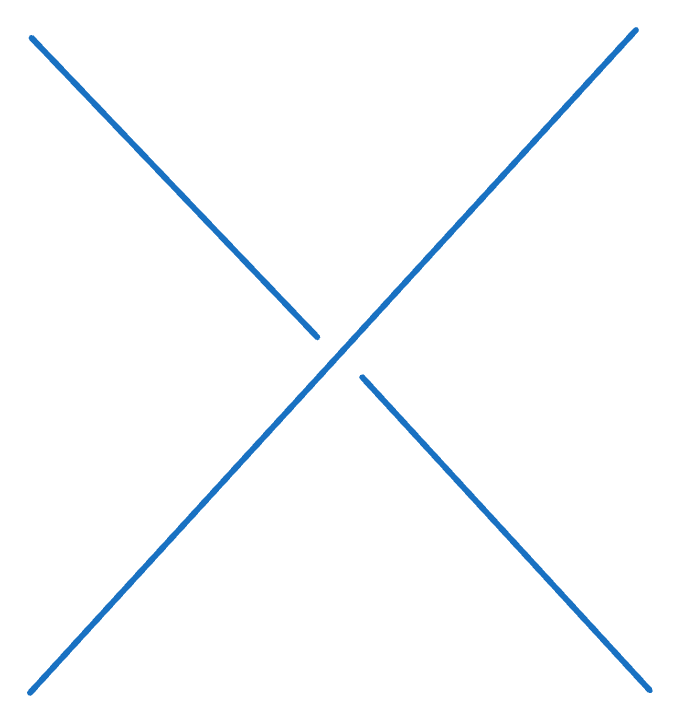
\includegraphics[width=9em]{figs/b2e145_1.png}&
		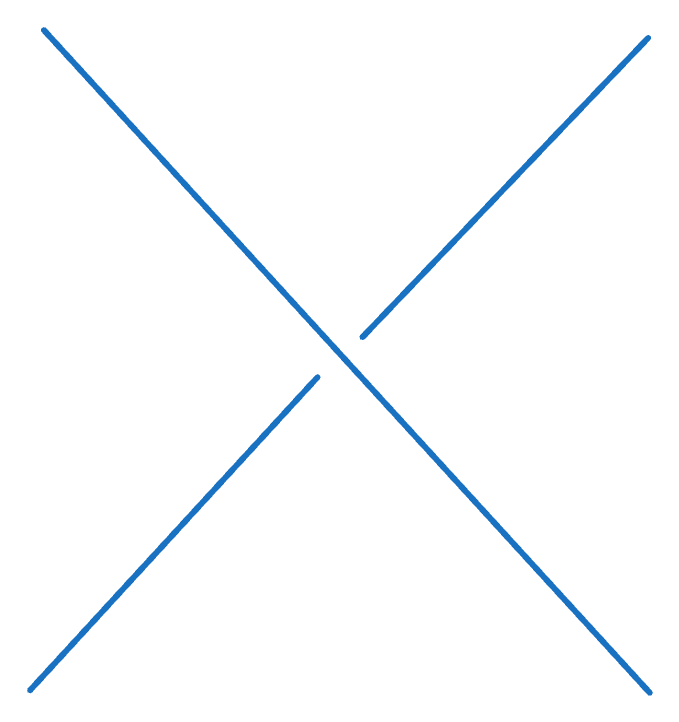
\includegraphics[width=9em]{figs/b2e145_2.png}\\
		$L$&$L^*$
	\end{tabular}
\end{center}
and
\begin{center}
	\begin{tabular}{ c | c} 
		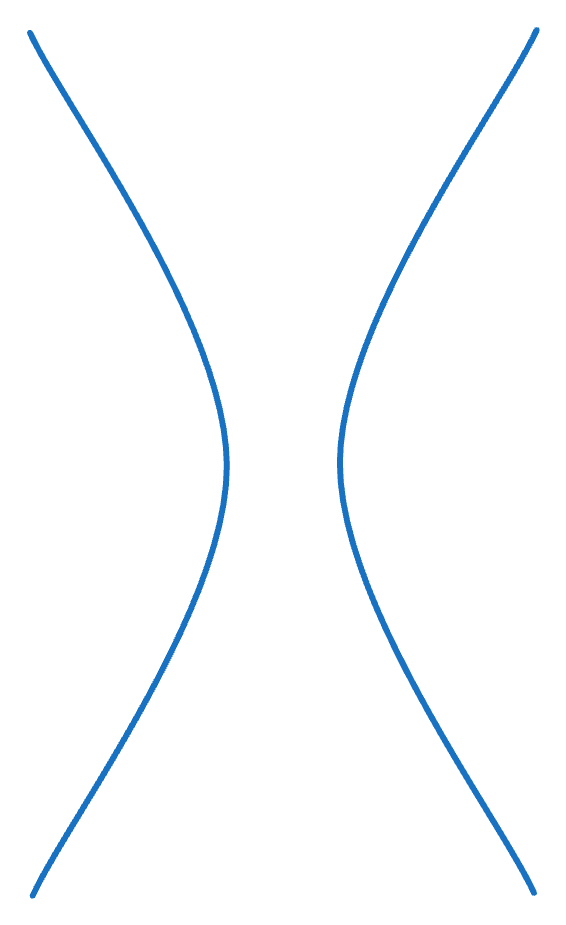
\includegraphics[width=5em]{figs/b2e145_3.png}&
		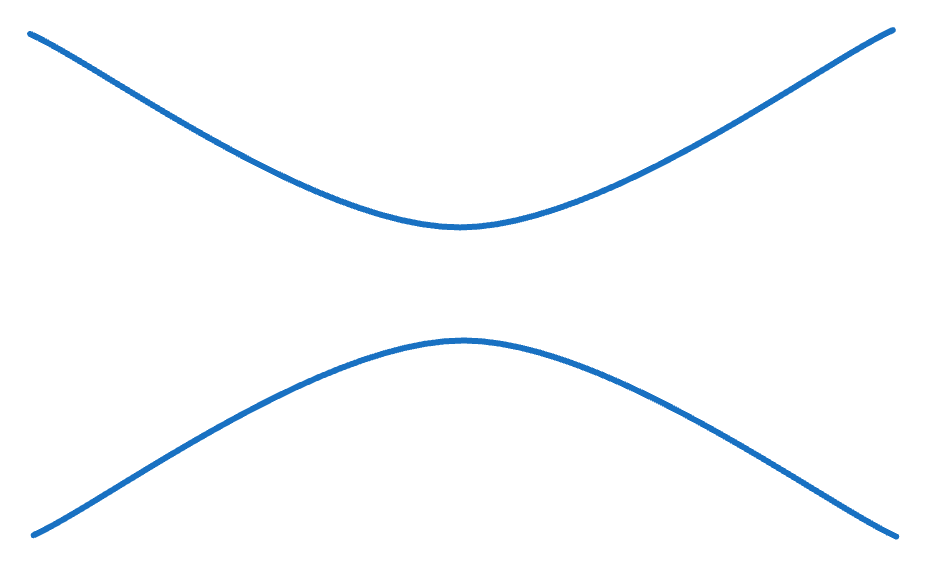
\includegraphics[width=9em]{figs/b2e145_4.png}\\
		$L$&$L^*$
	\end{tabular}
\end{center}
From the skein relations of Kauffman bracket it quickly follows that $\bk{L^*}(A)=\bk{L}(A^{-1})$.


\begin{example}
	Calculate $\bk{K}$ for the figure-eight knot $K$ shown in Fig 8. Check that $\bk{K}(A)=\bk{K}(A^{-1})$, which is consistent with the above Ex \ref{b2e144} and the the fact, shown in Ex \ref{b2e129}, that $K$ is regular-isotopic to its mirror image.
\end{example}
\sol $$
\begin{aligned}
	\bk*{\mims{figs/b2e146_1.png}{9em}} &= A\bk*{\ub{\mims{figs/b2e146_2.png}{9em}}{\text{Trefoil from Ex \ref{b2e144}}}}+A^{-1}\bk*{\ub{\mims{figs/b2e146_3.png}{9em}}{\text{Undo right-handed twist}}}\\
	&=A[-(A^2+A^{-2})(-A^7-A^{3}+A^{-5})] + A^{-1} (-A^3)\bk*{\ub{\mims{figs/b2e143_2.png}{9em}}{\text{Hopf link}}}\\
	% A[-(A^2+A^{-2})(-A^7-A^{3}+A^{-5})] + A^{-1} (-A^3)((A^2+A^{-2})^3-2(A^2+A^{-2}))\\
	&= -(A^2+A^{-2})(A^8-A^4-A^{-4}+1+A^{-8})
\end{aligned}
$$
Using the result from Ex \ref{b2e145}, we calculate the bracket of the mirror image as
$$
\begin{aligned}
	\bk{K}(A^{-1}) &= -(A^{-2}+A^{2})(A^{-8}-A^{-4}-A^{4}+1+A^{8})\\
	&= -(A^2+A^{-2})(A^8-A^4-A^{-4}+1+A^{-8})\\
	&= \bk{K}(A)
\end{aligned}
$$
once again showing that the figure-eight knot is amphichiral.


\begin{example}
	Derive the skein relations for the Jones polynomial.
\end{example}
\sol Notice that for $R=\mims{figs/rh.png}{4em},X = \mims{figs/dd.png}{1.5em},Y = \mims{figs/b2e145_4.png}{4em}$:
$$
\begin{aligned}
	A^4 V_R(A) &= A^4(-A^{-3})^{w(R)}\bk{R}(A)\\
	&= -A(A\bk{X}(A)+A^{-1}\bk{Y}(A))\\
	&= -A^2\bk{X}(A)-\bk{Y}(A)\\
	&= -A^2 V_X(A)- V_Y(A)\marginnote{(1)}
\end{aligned}$$
Similarly for $L=\mims{figs/lh.png}{4em}, X = \mims{figs/dd.png}{1.5em},Y = \mims{figs/b2e145_4.png}{4em}$:
$$
A^{-4} V_L(A) = -V_Y(A)- A^{-2}V_X(A)\marginnote{(2)}
$$
Subtracting (1) - (2) gives us the first skein relation:
$$
	A^{-4} V_R(A) - A^{4} V_L(A) = (A^2-A^{-2}) V_X(A)
$$
For $O=\mims{figs/circ_l.png}{4em}$, we have that $\bk{L \cup O} = -(A^2+A^{-2})(-A^3)^{w(O)}\bk{L}$ for all links $L$, so every twist that generates an unknot gets cancelled out by the $(-A^{-3})^{w(L)}$ factor in the definition of the Jones polynomial.
This gives us the second skein relation:
$$
	V_O(A)=1
$$

\begin{definition}
	There is a similarity between generating functionals in quantum physics, and partition functions in statistical physics. This similarity can be exploited by making the substitution\marginnote{Ref [35], Ch 25}
	$
	\frac{\di t}{\hbar} \to \frac{1}{k_BT},
	$
	and the claim is that this will map a quantum field theory on to a statistical field theory. This transformation is known as a \tb{Wick rotation} and leads to a very nice feature for spacetime four-vectors. By rotating the time-like part we can transform the Minkowski metrics $(+,-,-,-)$ or $(-,+,+,+)$ into the familiar Euclidean metric $(+,+,+,+)$, with an overall minus sign in the first case.
\end{definition}






% ----------------------------------------------------------------------
%           Book 3
% ----------------------------------------------------------------------
\newpage
\part{Gravity}






\section{Semi-Riemannian Geometry}\label{b3c1}



\begin{example}\label{b3e1}
	Show that this follows.\mn{If we have an $(r,s)$-tensor field $X$, we can pair or \tb{contract} the $i$th vector field with the $j$th 1-form to get an $(r-1,s-1)$-tensor field $Y$.}
\end{example}
\sol We can represent $X$ and $Y$ as a section of a tensor bundle:
$$
\begin{aligned}
	X &= v_1\otimes\cdots\otimes v_r\otimes \omega_1\otimes\cdots\otimes \omega_s\\\\
	Y &= \omega_j(v_i)\:v_1\otimes\cdots\hat{v}_i\cdots\otimes v_r\otimes \omega_1\otimes\cdots\hat{\omega}_j\cdots\otimes \omega_s
\end{aligned}
$$
This is given in local coordinates by
$$
\begin{aligned}
	X &= X(\omega_1,\cdots,\omega_r,v_1,\cdots,v_s)\\
	&= X_{\beta_1\cdots\beta_s}^{\alpha_1\cdots\alpha_r}\omega_{1_{\alpha_1}}\cdots\omega_{r_{\alpha_r}}v_1^{\beta_1}\cdots v_s^{\beta_s}\marginnote{Keep in mind $\alpha,\beta$ play the role of contravariant/covariant indices, whereas $i,j$ used within $v,\omega$ just index the arguments of the tensor.}\\\\
	Y &= Y(\omega_1,\cdots,\hat{\omega}_i,\cdots,\omega_r,v_1,\cdots,\hat{v}_j,\cdots,v_s)\\
	&= Y_{\beta_1\cdots\hat{\beta}_j\cdots\beta_s}^{\alpha_1\cdots\hat{\alpha}_i\cdots\alpha_r}\omega_{1_{\alpha_1}}\cdots\hat{\omega}_{i_{\alpha_i}}\cdots\omega_{r_{\alpha_r}}v_1^{\beta_1}\cdots \hat{v}_j^{\beta_j}\cdots v_s^{\beta_s}
\end{aligned}
$$
where the tensor components $X_{\beta_1\cdots\beta_s}^{\alpha_1\cdots\alpha_r}$ must contract/act on what is coming after it to produce a 0-form/function. In particular
$$
X_{\beta_1\cdots\beta_s}^{\alpha_1\cdots\alpha_r} = v_1^{\alpha_1}\cdots v_r^{\alpha_r}\omega_{1_{\beta_1}}\cdots\omega_{s_{\beta_s}}
$$
and therefore
$$
\begin{aligned}
	Y_{\beta_1\cdots\hat{\beta}_j\cdots\beta_s}^{\alpha_1\cdots\hat{\alpha}_i\cdots\alpha_r} &= \omega_{j_\mu}v_i^\mu v_1^{\alpha_1}\cdots\hat{v}_i^{\alpha_i}\cdots v_r^{\alpha_r}\omega_{1_{\beta_1}}\cdots\hat{\omega}_{j_{\beta_j}}\cdots\omega_{s_{\beta_s}}\\
	&= v_1^{\alpha_1}\cdots v_i^\mu\cdots v_r^{\alpha_r}\omega_{1_{\beta_1}}\cdots\omega_{j_\mu}\cdots\omega_{s_{\beta_s}}\\
	&= X_{\beta_1\cdots\mu\cdots\beta_s}^{\alpha_1\cdots\mu\cdots\alpha_r}
\end{aligned}
$$


\begin{example}
	The tangent bundle of $\R^n$ is trivial, with a basis of sections being given by the coordinate vector fields $\partial_\alpha$; thus it has a standard flat connection $D^0$ as described in Sec \ref{b2c2}. Show that this is the Levi-Civita connection for the standard metric of signature $(p,q)$ on $\R^n$,
	$$
	g=dx_1^2+\cdots+dx_p^2-dx_{p+1}^2-\cdots-dx_{p+q}^2.
	$$
	In particular, this applies of Euclidean $\R^n$ on Minkowski spacetime. More generally, show it is true for any metric on $\R^n$ such that the components $g_{\alpha\beta}$ with respect to the coordinate vector fields are constant.
\end{example}
\sol Write $g=g_{\alpha\beta}dx^\alpha dx^\beta$. Any vector fields on $\R^n$ can be represented in terms of the coordinate vector fields, i.e., $x=x^i\partial_i$.\\\\
For $u,v,w \in \Vect(M)$ we aim to show that the flat connection $D_u^0v=u^i\partial_iv$ is the Levi-Civita connection for any metric on $\R^n$. For this we have to prove the two properties on Pg 372 of the text:
\begin{enumerate}
	\item \underline{Metric preserving:}\\\\
	$$
	\begin{aligned}
		ug(v,w) &= u^\alpha\partial_\alpha(g_{\beta\gamma}v^\beta w^\gamma)\\
		&= u^\alpha g_{\beta\gamma}(\partial_\alpha v^\beta) w^\gamma + u^\alpha g_{\beta\gamma}v^\beta(\partial_\alpha w^\gamma)\\
		&= g(D_u^0v,w) + g(u,D_u^0w)
	\end{aligned}
	$$
	\item \underline{Torsion free:}\\\\
	$$
	\begin{aligned}
		[v,w] &= [v^\alpha\partial_\alpha,w^\beta\partial_\beta]\\
		&= v^\alpha\partial_\alpha(w^\beta\partial_\beta) - w^\beta\partial_\beta(v^\alpha\partial_\alpha)\\
		&= v^\alpha\partial_\alpha w - w^\beta\partial_\beta v\\
		&= D_v^0w - D_w^0v
	\end{aligned}
	$$
\end{enumerate}


\begin{example}\label{b3e3}
	Show that for the Levi-Civita connection $\nabla$, the Christoffel symbols are given by
	$$
	\Gamma_{\alpha\beta}^\gamma = \frac12 g^{\gamma\delta}(\partial_\alpha g_{\beta\delta}+\partial_\beta g_{\delta\alpha}-\partial_\delta g_{\alpha\beta}).
	$$
\end{example}
\sol Derived from the \emph{Koszul formula} on the bottom of Pg 373 of the text, we are led to this formula on Pg 374:
$$
\begin{aligned}
	2g_{\delta\gamma}\Gamma_{\alpha\beta}^\delta &= \partial_\alpha g_{\beta\gamma}+\partial_\beta g_{\gamma\alpha}-\partial_\gamma g_{\alpha\beta}\\
	\Rightarrow 2g_{\gamma\delta}\Gamma_{\alpha\beta}^\gamma &= \partial_\alpha g_{\beta\delta}+\partial_\beta g_{\delta\alpha}-\partial_\delta g_{\alpha\beta}\marginnote{Swap labels $\delta\leftrightarrow\gamma$}\\
	\Rightarrow \ub{g^{\gamma\delta}g_{\gamma\delta}}{\id}\Gamma_{\alpha\beta}^\gamma &= \frac12 g^{\gamma\delta}(\partial_\alpha g_{\beta\delta}+\partial_\beta g_{\delta\alpha}-\partial_\delta g_{\alpha\beta})\marginnote{$g^{\gamma\delta}=g_{\gamma\delta}^{-1}$}\\
	\Rightarrow \Gamma_{\alpha\beta}^\gamma &= \frac12 g^{\gamma\delta}(\partial_\alpha g_{\beta\delta}+\partial_\beta g_{\delta\alpha}-\partial_\delta g_{\alpha\beta})
\end{aligned}
$$


\begin{example}\label{b3e4}
	More generally, suppose we are working with an arbitrary basis of vector fields $e_\alpha$, satisfying\mn{$c_{\alpha\beta}^\gamma$ are also called the \tb{structure functions}}
	$$
	[e_\alpha,e_\beta]=c_{\alpha\beta}^\gamma e_\gamma.
	$$
	Defining
	$$
	\nabla_\alpha=\nabla_{e_\alpha},\qquad\nabla_\alpha e_\beta-\Gamma_{\alpha\beta}^\gamma e_\gamma,
	$$
	and
	$$
	\Gamma_{\gamma\alpha\beta}=g_{\gamma\delta}\Gamma_{\alpha\beta}^\delta,\qquad c_{\gamma\alpha\beta}=g_{\gamma\delta}c_{\alpha\beta}^\delta,
	$$
	show that
	$$
	\Gamma_{\gamma\alpha\beta}=\frac12({\color{red}e}_\alpha g_{\beta\gamma}+{\color{red}e}_\beta g_{\gamma\alpha}-{\color{red}e}_\gamma g_{\alpha\beta}+c_{\gamma\alpha\beta}{\color{red}-c_{\beta\alpha\gamma}}-c_{\alpha\beta\gamma}).
	$$
\end{example}
\sol Starting from the Koszul formula, we defer to Ref [1], Pg 202, Thm 8.6 to prove our result. It shows that the Christoffel symbols are determined uniquely by the metric tensor and the structure functions. We highlight some corrections to the main text in {\color{red}red}, and make the following notes:
\begin{itemize}
	\item Writing \marginnote{Ref [1], Pg 194 and Eq (8.39)}$\Gamma$ in terms of $\partial$s $\Rightarrow e_\alpha = \partial_\alpha \Rightarrow [e_\alpha,e_\beta]=0 \Rightarrow \br{e_\alpha}$ is a locally holonomic basis $\Rightarrow$ the structure functions vanish.
	\item The antisymmetry of the Lie bracket does not imply antisymmetry of $\Gamma_{\gamma\alpha\beta}$, $\Gamma_{\alpha\beta}^\gamma$, $c_{\gamma\alpha\beta}$ or $c_{\alpha\beta}^\gamma$. But it may be that $c_{\gamma\alpha\beta} = -c_{\gamma\beta\alpha}$. See this applied in Ex \ref{b3e5}.
\end{itemize}


\begin{example}\label{b3e5}
	Show that in a basis of coordinate vector fields we have
	$$
	\Gamma_{\beta\gamma}^\alpha=\Gamma_{\gamma\beta}^\alpha
	$$
	while in an orthonormal basis, e.g. one in which $g(e_\alpha,e_\beta)$ is zero if $\alpha\ne\beta$ and $\pm 1$ if $\alpha=\beta$, we have
	$$
	\Gamma_{\alpha\beta\gamma}=-\Gamma_{\gamma\beta\alpha}.
	$$
\end{example}
\sol Cyclically permuting the labels ($\alpha \to \beta,\: \beta \to \gamma,\: \gamma \to \alpha$) in Ex \ref{b3e3}:
$$
\begin{aligned}
	\Gamma_{\beta\gamma}^\alpha &= \frac12 g^{\alpha\delta}(\ub{\partial_\beta g_{\gamma\delta}+\partial_\gamma g_{\delta\beta}}{\text{Swap}}-\partial_\delta g_{\beta\gamma})\\
	&= \frac12 g^{\alpha\delta}(\partial_\gamma g_{\delta\beta}+\partial_\beta g_{\gamma\delta}-\partial_\delta g_{\beta\gamma})\\
	&= \frac12 g^{\alpha\delta}(\partial_\gamma g_{\beta\delta}+\partial_\beta g_{\delta\gamma}-\partial_\delta g_{\gamma\beta})\marginnote{Metric tensor is always symmetric: $g_{ij} = g_{ji}$}\\
	&= \Gamma_{\gamma\beta}^\alpha
\end{aligned}
$$
Adopting notation from Pg 375 of the text, and using corrections from Ex \ref{b3e4}:
$$
\begin{aligned}
	\Gamma_{\alpha\beta\gamma} &= \frac12(\ub{g_{\alpha\beta,\gamma}+g_{\gamma\alpha,\beta}-g_{\beta\gamma,\alpha}}{= 0 \text{ ($g$ is constant)}}+c_{\alpha\beta\gamma}-c_{\gamma\beta\alpha}-c_{\beta\gamma\alpha})\\
	&= \frac12(c_{\alpha\beta\gamma}-c_{\gamma\beta\alpha}-c_{\beta\gamma\alpha})\\
	&= -\frac12(c_{\gamma\beta\alpha}-c_{\alpha\beta\gamma}-c_{\beta\alpha\gamma})\marginnote{Swap first two terms, in the third term swap indices $\alpha\leftrightarrow\gamma$ giving a minus sign}\\
	&= -\Gamma_{\gamma\beta\alpha}
\end{aligned}$$
Where we used a property that structure functions with all downstairs indices are antisymmetric, atleast in swapping the last two indices. TODO find out why and in which indices.

\begin{example}\label{b3e6}
	Compute the Christoffel symbols on $S^2$ in spherical coordinates, with the standard metric
	$$
	d\phi^2+\sin^2\phi d\theta^2.
	$$
	Do the same for the spacetime $\R^4$ using spherical coordinates on space, with the metric
	$$
	g=-f(r)^2dt^2+f(r)^{-2}dr^2+r^2(d\phi^2+\sin^2\phi d\theta^2)
	$$
	(Up to a change of coordinates, this is basically a spacetime version of the wormhole metric considered in Sec \ref{b1c6}.)
\end{example}
\sol See {\tt data/nb/b3e6.nb} which uses the OGRe (Ref [36]) library to calculate and show the nonzero Christoffel symbols.\\\\
For the \underline{standard metric} on $S^2$ we have\marginnote{Detailed calculation in Ref [1], Pg 203, Ex 8.5}
$$
\mims{figs/b3e6_1.pdf}{16em}
$$
and for the \underline{wormhole metric} on $\R^4$
$$
\mims{figs/b3e6_2.pdf}{20em}
$$


\begin{example}
	Prove that this sort of formula\mn{For $(r, s)$ tensor field $X$, find the components of its covariant derivative $\nabla_\mu X$ in terms of partial derivatives of the components of $X$ and Christoffel symbols.} holds for arbitrary $(r,s)$-tensors.
\end{example}
\sol For vector fields $v,w \in \Vect(M)$ the formula on Pg 374 of the text
$$
\nabla_v w=v^\alpha\ub{(\partial_\alpha w^\beta+\Gamma_{\alpha\gamma}^\beta w^\gamma)}{(\nabla_\alpha w)^\beta}\partial_\beta
$$
gives us the component of the Levi-Civita connection of $w$ in the direction of $v$. We aim to find a similar expression for covector field $\omega$. For this we need two properties of the covariant derivative for some $f \in C^\infty(M)$ and $\omega \in \Omega^1(M)$:\marginnote{Ref [1], Pg 183, (C4), (C5)}
\begin{itemize}
	\item Reduction to ordinary derivative on functions: $\nabla_v f = v(f)$
	\item Compatibility with dual pairing: $\nabla_v\bk{w,\omega}=\bk{\nabla_v w,\omega}+\bk{w,\nabla_v\omega}$
\end{itemize}
Using these along with the definition of the Christoffel symbols gives
$$
\begin{aligned}
	0 &= \nabla_\alpha\bk{\partial_\beta, dx^\gamma}\marginnote{Ref [1], Ex 8.3}\\
	&= \bk{\nabla_\alpha\partial_\beta, dx^\gamma} + \bk{\partial_\beta,\nabla_\alpha dx^\gamma}\\
	&= \bk{\Gamma_{\alpha\beta}^\gamma\partial_\gamma, dx^\gamma} + \bk{\nabla_\alpha dx^\gamma,\partial_\beta}\marginnote{Pg 374 of the text}\\
	&= \ub{g_{\gamma\gamma}}{1}\Gamma_{\alpha\beta}^\gamma\cancel{\partial_\gamma dx^\gamma} + \ub{g^{\beta\beta}}{1}\nabla_\alpha dx^\gamma\partial_\beta\marginnote{TODO Explain $g^{\beta\beta}$ here}\\
	\Rightarrow \nabla_\alpha dx^\gamma \partial_\beta &=-\Gamma_{\alpha\beta}^\gamma\\
	\Rightarrow \nabla_\alpha dx^\gamma \cancel{\partial_\beta dx^\beta}&=-\Gamma_{\alpha\beta}^\gamma dx^\beta\\
	\Rightarrow \nabla_\alpha dx^\gamma&=-\Gamma_{\alpha\beta}^\gamma dx^\beta
\end{aligned}
$$
% , and we will call that Christoffel symbol $\tilde{\Gamma}$.\\\\
% Starting with a (0,0) tensor field (i.e. scalar field), we note that we can express any scalar $c$ as an inner product (i.e. tensor contraction): $c = \omega(v) = \omega_\nu v^\nu$. Because the covariant derivative of $c$ is equal to the partial derivative, we have
% $$
% \begin{aligned}
% 	\nabla_\mu(c)&=\nabla_\mu(\omega_\nu v^\nu)\\
% 	&=(\nabla_\mu\omega_\nu) v^\nu+\omega_\nu (\nabla_\mu v^\nu)\\
% 	&=(\partial_\mu\omega+) v^\nu+\omega_\nu (\nabla_\mu v^\nu)\\
% \end{aligned}
% $$
We have seen the covariant derivative for (1,0), (0,1) tensors and we now show it for a (1,1)-tensor field $T=T_j^i\partial_i\otimes dx^j$:
$$
\begin{aligned}
	\nabla_k T &= \partial_k(T_j^i)\partial_i\otimes dx^j + T_j^i\nabla_k(\partial_i)\otimes dx^j+ T_j^i\partial_i\otimes \nabla_k(dx^j)\marginnote{Ref [1], Pg 225, Ex 8.31}\\
	&= T_{j,k}^i\partial_i\otimes dx^j + T_{\textcolor{blue}j}^{\textcolor{green}i}\Gamma_{k{\textcolor{green}i}}^{\textcolor{red}\ell}\partial_{\textcolor{red}\ell}\otimes dx^{\textcolor{blue}j}- T_{\textcolor{green}j}^{\textcolor{red}i}\partial_{\textcolor{red}i}\otimes \Gamma_{k{\textcolor{blue}\ell}}^{\textcolor{green}j}dx^{\textcolor{blue}\ell}\\
	&= T_{j,k}^i\partial_i\otimes dx^j + T_{\textcolor{blue}j}^{\textcolor{green}\ell}\Gamma_{k{\textcolor{green}\ell}}^{\textcolor{red}i}\partial_{\textcolor{red}i}\otimes dx^{\textcolor{blue}j}- T_{\textcolor{green}\ell}^{\textcolor{red}i}\partial_{\textcolor{red}i}\otimes \Gamma_{k{\textcolor{blue}j}}^{\textcolor{green}\ell}dx^{\textcolor{blue}j}\\
	&= (T_{j,k}^i + \Gamma_{k{\ell}}^{i}T_{j}^{\ell} - \Gamma_{k{j}}^{\ell}T_{\ell}^{i})\partial_i\otimes dx^j
\end{aligned}
$$
Where we go from step 2 to 3 by relabelling indices in such a way that the internal contraction marked in \textcolor{green}{green} and contractions with $\partial$ and $dx$ marked in \textcolor{red}{red} and \textcolor{blue}{blue} respectively remain the same. After doing this we can factor out the tensor product.\\\\
Expressing this result using the notation $X=X_\beta^\alpha\partial_\alpha\otimes dx^\beta$ form the text:
$$
	\nabla_\mu X = (X_{\beta,\mu}^\alpha+\Gamma_{\mu\lambda}^\alpha X_\beta^\lambda-\Gamma_{\mu\beta}^\lambda X_\lambda^\alpha)\partial_\alpha\otimes dx^\beta
$$
Arbitrary $(r,s)$-tensors follow by induction:
$$
	\nabla_\mu X = (X_{\beta_1\cdots\beta_s,\mu}^{\alpha_1\cdots\alpha_r}\ub{+\Gamma_{\mu\lambda}^{\alpha_1} X_{\beta_1\cdots\beta_s}^{\lambda\alpha_2\cdots\alpha_r}+\cdots+\Gamma_{\mu\lambda}^{\alpha_r} X_{\beta_1\cdots\beta_s}^{\alpha_1\cdots\alpha_{r-1}\lambda}}{r\text{ times}}\ub{-\Gamma_{\mu\beta_1}^\lambda X_{\lambda\beta_2\cdots\beta_s}^{\alpha_1\cdots\alpha_r}-\cdots-\Gamma_{\mu\beta_s}^\lambda X_{\beta_1\cdots\beta_{s-1}\lambda}^{\alpha_1\cdots\alpha_r}}{s\text{ times}})\partial_\alpha\otimes dx^\beta
$$
We have used the Leibniz law for covariant derivatives of tensor products which is proved in Ex \ref{b3e8}.


\begin{example}\label{b3e8}
	Show that the covariant derivative $\nabla$ satisfies linearity
	$$
	\nabla(cX)=c\nabla X,\qquad \nabla(X+X^\prime)=\nabla X+\nabla X^\prime
	$$
	(where $c$ is a scalar), the generalized Leibniz law
	$$
	\nabla_\mu(X \otimes X^\prime) = \nabla_\mu X \otimes X^\prime + X \otimes  \nabla_\mu X^\prime,
	$$
	and compatibility with contraction: if $Y$ is obtained from $X$ by constructing indices as follows,
	$$
	Y_{\beta_1\cdots\hat{\beta}_j\cdots\beta_s}^{\alpha_1\cdots\hat{\alpha}_i\cdots\alpha_r}=X_{\beta_1\cdots\mu\cdots\beta_s}^{\alpha_1\cdots\mu\cdots\alpha_r},
	$$
	then
	$$
	\nabla_\rho Y_{\beta_1\cdots\hat{\beta}_j\cdots\beta_s}^{\alpha_1\cdots\hat{\alpha}_i\cdots\alpha_r}=\nabla_\rho X_{\beta_1\cdots\mu\cdots\beta_s}^{\alpha_1\cdots\mu\cdots\alpha_r}.
	$$
	Also, we define the covariant derivative of a (0,0)-tensor to be its differential,
	$$
	\nabla f = df,
	$$
	and define it to agree with the Levi-Civita connection on (1,0)-tensors. Show that $\nabla$ is uniquely determined by the above properties.
\end{example}
\sol This covariant derivative ($\nabla$ without a subscript) is also called the total covariant derivative. The point is that $\nabla X$ contains the information of $\nabla_\mu X$ for every choice of $\partial_\mu$. Since $\nabla X= dx^\mu \otimes \nabla_\mu X$, it can be defined using the connection. Pg 223 of the text shows linearity of the connection and thus $\nabla$.\\\\
See Ref [37] for why there is no Leibniz rule for total covariant derivatives.\\\\
The next property follows from Ex \ref{b3e1}, just add a covariant derivative.\\\\
The proof of existence and uniqueness of the exterior derivative/differential is carried out in Ref [3], Pg 365, Thm 14.24.


\begin{example}
	Show that the great circles on the sphere $S^2$ are geodesics with respect to its standard metric.
\end{example}
\sol See the following in Ref [1] for the main proof:
\begin{marginfigure}
	\begin{center}
	  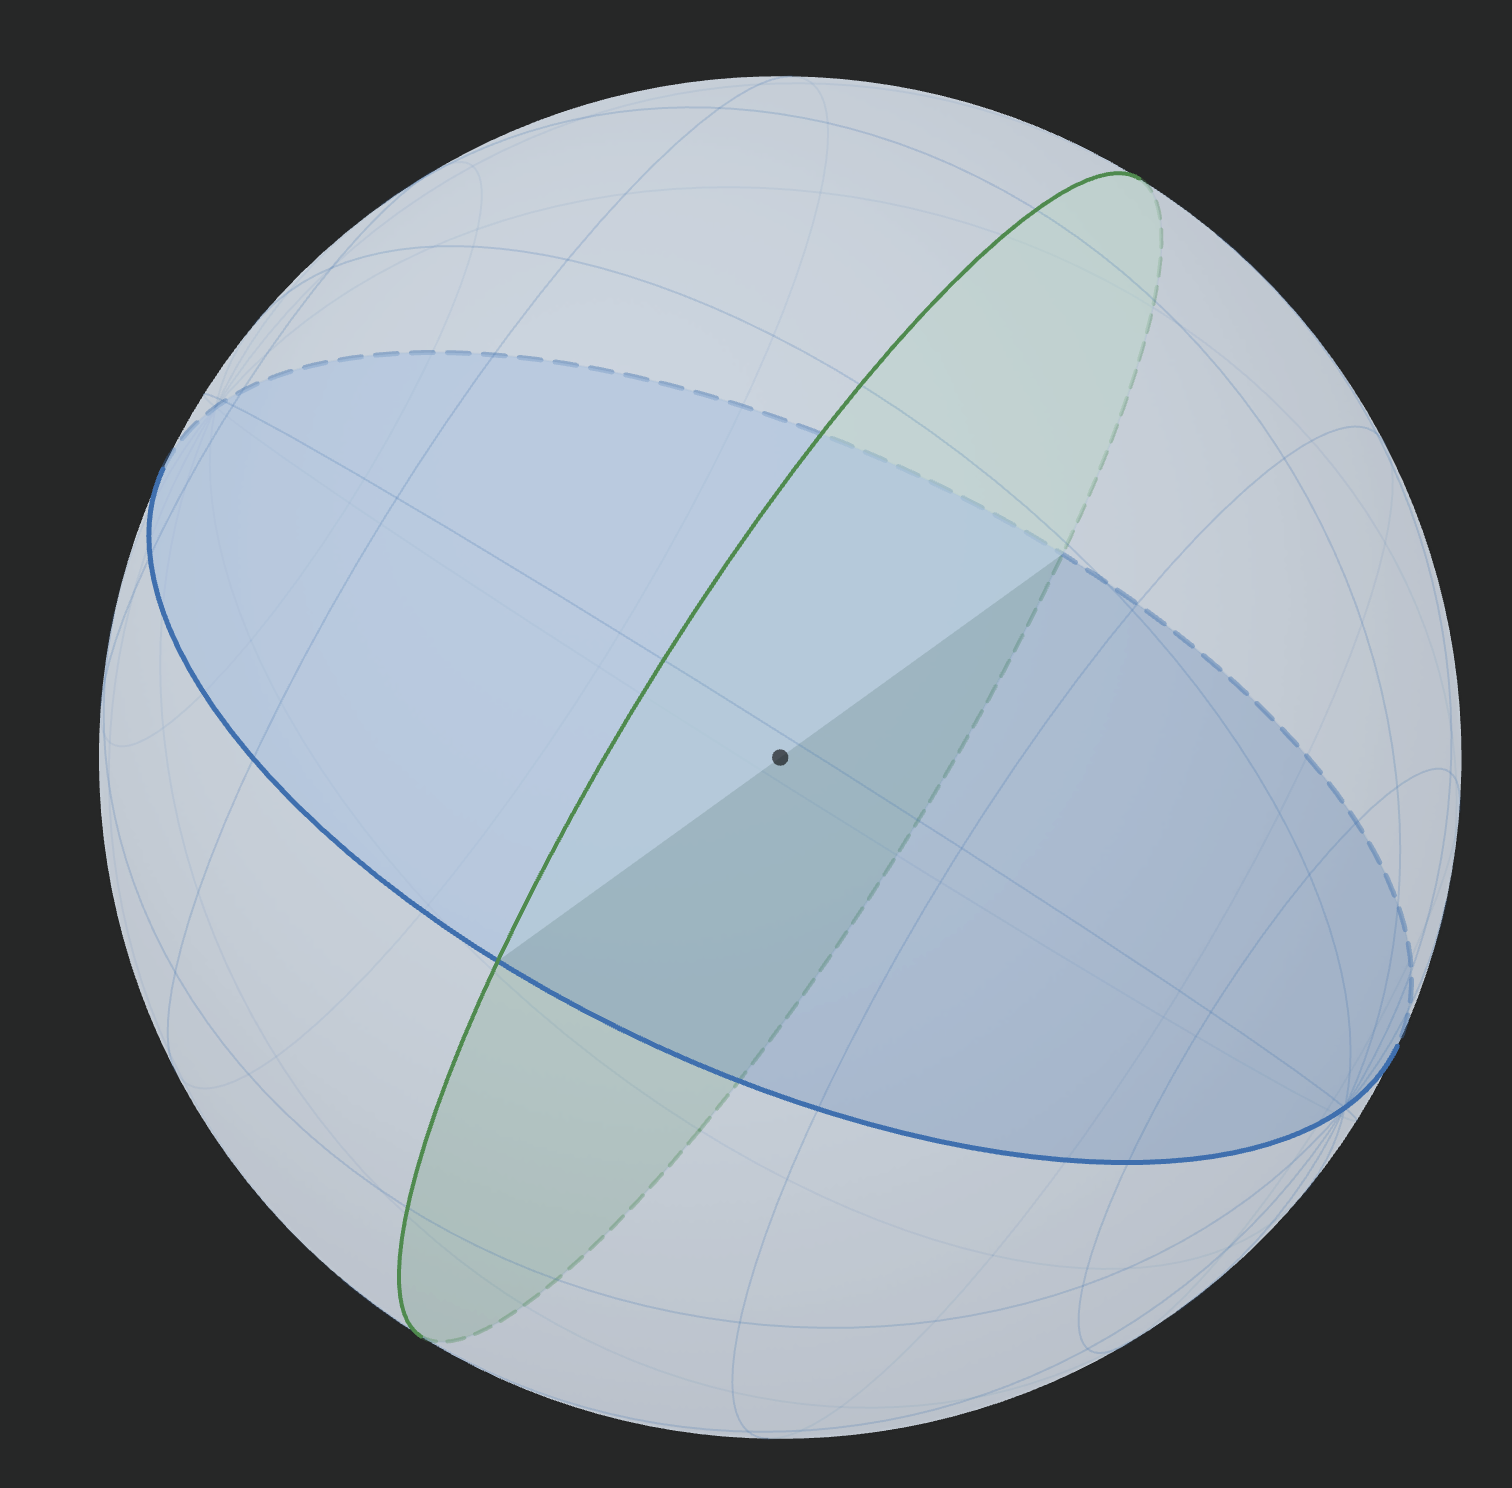
\includegraphics[width=1.2\textwidth]{figs/great_circ.png}
	\end{center}
	\caption{Great circles on $S^2$}
\end{marginfigure}
\begin{itemize}
	\item Ex 8.47
	\item Ex 8.5
	\item Ex 8.42 (main calculation)
\end{itemize}
An alternative proof for the general case of $S^n$ that does not use Christoffel symbols is given in Ref [23], Pg 82, Prop 5.13.\\\\
The main proof involves plugging in the Christoffel symbols from Ex \ref{b3e6} into the geodesic equations on Pg 379 of the text
$$
\frac{d^2\gamma^\mu}{dt^2}+\Gamma_{\nu\lambda}^\mu\frac{d\gamma^\nu}{dt}\frac{d\gamma^\lambda}{dt}=0
$$
where the indices $\mu,\nu,\lambda \in \br{\theta,\phi}$. This gives us a coupled pair of second-order differential equations (one for $\mu\ne\lambda$, one for $\mu=\lambda$) that can be reduced to first-order.\\\\
When solved, we get more or less that the great circles are parametrized by the curve 
$$\gamma:[0,1]\to\begin{pmatrix}
	\gamma^\phi\\\gamma^\theta
\end{pmatrix}=\begin{pmatrix}
	\phi_0 \\2\pi t
\end{pmatrix}
$$
for constant $\phi_0 \in [0,2\pi]$.\\\\
Transforming the solutions to Cartesian coordinates gives
$$z = C \cos(\phi_0) y - C \sin(\phi_0)x$$
where $C \in \R^+$. This is the equation of a plane passing through the origin. The geodesics are the intersections of this plane with the sphere, namely great circles.


\begin{example}
	Do the computation\mn{If $\gamma$ is a path and $v(t),w(t)$ are two vectors parallel transported along $\gamma$, we claim$$\frac{d}{dt}g(v(t),w(t))=0$$}.
\end{example}
\sol We know that if $\nabla$ is metric preserving
$$
\nabla_{\gamma^\prime(t)}g(v(t),w(t)) = g(\ub{\nabla_{\gamma^\prime(t)}v(t)}{=0},w(t)) +g(v(t),\ub{\nabla_{\gamma^\prime(t)}w(t)}{=0}) = 0
$$
by the definition of parallel transport.\\\\
On the 1-dimensional manifold $\gamma(t)$, covariant derivative w.r.t tangent vector boils down to standard derivative w.r.t curve parameter, so
$$\nabla_{\gamma^\prime(t)}g(v(t),w(t)) = \frac{d}{dt}g(v(t),w(t))=0$$
Since the length of $v$ is $\sqrt{g(v,v)}$ and the cosine of the angle between $v$ and $w$ is $g(v, w)/\sqrt{g(v,v)g(w, w)}$, for parallel transported vectors these quantities are constant along the curve.


\begin{example}\label{b3e11}
	Calculate the Riemann tensor, the Ricci tensor, the Ricci scalar and Einstein tensor for the standard metric on $S^2$, starting with the results of Ex \ref{b3e6}. Do the same for the spacetime metric
	$$
	g=-f(r)^2dt^2+f(r)^{-2}dr^2+r^2(d\phi^2+\sin^2\phi d\theta^2)
	$$
	This takes some work, but in the next chapter you can use these computations to work out the metric describing a black hole!
\end{example}
\sol See {\tt data/nb/b3e11.nb}.\\\\
For \underline{standard metric} on $S^2$ we have
$$
\mims{figs/b3e11_1.pdf}{16em}
$$
$$
\mims{figs/b3e11_2.pdf}{12em}
$$
$$
\mims{figs/b3e11_3.pdf}{12em}
$$
and for the \underline{wormhole metric} on $\R^4$
$$
\mims{figs/b3e11_4.pdf}{30em}
$$
$$
\mims{figs/b3e11_5.pdf}{22em}
$$
$$
\mims{figs/b3e11_6.pdf}{25em}
$$


\begin{example}
	Show that $R_{\alpha\beta\gamma\delta}=g(e_\alpha,R(e_\beta,e_\gamma)e_\delta)$.
\end{example}
\sol $$
\begin{aligned}
	R_{\alpha\beta\gamma\delta}&=g_{\alpha\lambda}R_{\beta\gamma\delta}^\lambda\\
	&=g(e_\alpha,e_\lambda)R_{\beta\gamma\delta}^\lambda\\
	&=g(e_\alpha,R_{\beta\gamma\delta}^\lambda e_\lambda)\\
	&=g(e_\alpha,R(e_\beta,e_\gamma)e_\delta)
\end{aligned}$$


\begin{example}\label{b3e13}
	Write the relation $R_{\sparen{\beta\gamma\delta}}^\lambda=0$ in an explicit form, and simplify it using other symmetries.
\end{example}
\sol Using the symmetries on Pg 383 of the text
$$
\begin{aligned}
	0=R_{[\beta\gamma\delta]}^\lambda &= \frac{1}{3!} \p{
		R_{\beta\gamma\delta}^\lambda
		- R_{\beta\delta\gamma}^\lambda
		- R_{\gamma\beta\delta}^\lambda
		+ R_{\gamma\delta\beta}^\lambda
		+ R_{\delta\beta\gamma}^\lambda
		- R_{\delta\gamma\beta}^\lambda}\marginnote{See \tt{data/perm.ipynb}}\\
	&= \frac{1}{3!} \p{
		R_{\beta\gamma\delta}^\lambda
		+ R_{\delta\beta\gamma}^\lambda
		+ R_{\beta\gamma\delta}^\lambda
		+ R_{\gamma\delta\beta}^\lambda
		+ R_{\delta\beta\gamma}^\lambda
		+ R_{\gamma\delta\beta}^\lambda}\marginnote{Apply Symm 1 to the minus signs}\\
	&= \frac{1}{3} \p{
		R_{\beta\gamma\delta}^\lambda
		+ R_{\delta\beta\gamma}^\lambda
		+ R_{\gamma\delta\beta}^\lambda}\\
	&\Rightarrow R_{\beta\gamma\delta}^\lambda + R_{\delta\beta\gamma}^\lambda+ R_{\gamma\delta\beta}^\lambda=0\\
	&\Rightarrow R_{\alpha\beta\gamma\delta} + R_{\alpha\delta\beta\gamma}+ R_{\alpha\gamma\delta\beta}=0\marginnote{Lower using $g_{\alpha\lambda}$}
\end{aligned}$$
Summing up the cyclic permutations of the lower indices in square brackets goes to zero, even after the first index is lowered. This explicit form for Symm 3 is another rendition of the Bianchi identity.


\begin{example}\label{b3e14}
	Show that relations\mn{symmetries} 1-3 imply $R_{\alpha\beta\gamma\delta}=R_{\gamma\delta\alpha\beta}$ and $R_{\sparen{\alpha\beta\gamma\delta}}=0$.
\end{example}
\sol We state here a symmetry from Ref [38], Pg 160, Eq 6.69, and call it Symm 4:
$$
R_{\alpha\beta\gamma\delta} = -R_{\beta\alpha\gamma\delta} = -R_{\alpha\beta\delta\gamma}
$$
Symm 4 states that $R_{\alpha\beta\gamma\delta}$ is antisymmetric on the first pair and on the second pair of indices. Let's prove Symm 5, symmetry on exchange of the first and second pair. Here are all the versions of Symm 3
$$
\begin{aligned}
	R_{\alpha\beta\gamma\delta} + R_{\alpha\delta\beta\gamma}+ R_{\alpha\gamma\delta\beta}&=0\\
	R_{\beta\alpha\gamma\delta} + R_{\beta\delta\alpha\gamma}+ R_{\beta\gamma\delta\alpha}&=0\\
	R_{\gamma\alpha\beta\delta} + R_{\gamma\delta\alpha\beta}+ R_{\gamma\beta\delta\alpha}&=0\\
	R_{\delta\alpha\beta\gamma} + R_{\delta\gamma\alpha\beta}+ R_{\delta\beta\gamma\alpha}&=0\\
\end{aligned}
$$
Summing them up, some cancel out by applying some combination of either Symm 2 or Symm 4:
$$
\begin{aligned}
	R_{\alpha\beta\gamma\delta} + \cancelto{1}{R_{\alpha\delta\beta\gamma}}+ \cancelto{2}{R_{\alpha\gamma\delta\beta}}&\\
	+\cancelto{4}{R_{\beta\alpha\gamma\delta}} + \cancelto{3}{R_{\beta\delta\alpha\gamma}}+ \cancelto{2}{R_{\beta\gamma\delta\alpha}}&\\
	+\cancelto{4}{R_{\gamma\alpha\beta\delta}} + \cancelto{3}{R_{\gamma\delta\alpha\beta}}+ \cancelto{5}{R_{\gamma\beta\delta\alpha}}&\\
	+\cancelto{1}{R_{\delta\alpha\beta\gamma}} + R_{\delta\gamma\alpha\beta}+ \cancelto{5}{R_{\delta\beta\gamma\alpha}}&=0\\
\end{aligned}
$$
This leaves us with
$$
\begin{aligned}
	R_{\alpha\beta\gamma\delta} &= -R_{\delta\gamma\alpha\beta}\\
	\Rightarrow R_{\alpha\beta\gamma\delta} &= R_{\gamma\delta\alpha\beta}\marginnote{Symm 4}
\end{aligned}
$$
We now prove the next symmetry, which we call Symm 6:
$$\begin{alignedat}{3}
	R_{[\alpha\beta\gamma\delta]}&= \frac{1}{4!}&(R_{\alpha\beta\gamma\delta}
	- R_{\alpha\beta\delta\gamma}
	- R_{\alpha\gamma\beta\delta}
	+ R_{\alpha\gamma\delta\beta}
	+ R_{\alpha\delta\beta\gamma}
	- R_{\alpha\delta\gamma\beta}&\\
	&&- R_{\beta\alpha\gamma\delta}
	+ R_{\beta\alpha\delta\gamma}
	+ R_{\beta\gamma\alpha\delta}
	- R_{\beta\gamma\delta\alpha}
	- R_{\beta\delta\alpha\gamma}
	+ R_{\beta\delta\gamma\alpha}&\\
	&&+ R_{\gamma\alpha\beta\delta}
	- R_{\gamma\alpha\delta\beta}
	- R_{\gamma\beta\alpha\delta}
	+ R_{\gamma\beta\delta\alpha}
	+ R_{\gamma\delta\alpha\beta}
	- R_{\gamma\delta\beta\alpha}&\\
	&&- R_{\delta\alpha\beta\gamma}
	+ R_{\delta\alpha\gamma\beta}
	+ R_{\delta\beta\alpha\gamma}
	- R_{\delta\beta\gamma\alpha}
	- R_{\delta\gamma\alpha\beta}
	+ R_{\delta\gamma\beta\alpha}&)\\
	%%
	&= \frac{1}{4!}&2(R_{\alpha\beta\gamma\delta}\marginnote{Symm 2, 4}
	+ R_{\alpha\delta\beta\gamma}
	+ R_{\alpha\gamma\delta\beta})&\\
	&&+ 2(R_{\beta\delta\gamma\alpha}
	+ R_{\beta\alpha\delta\gamma}
	+ R_{\beta\gamma\alpha\delta})&\\
	&&+ 2(R_{\gamma\alpha\beta\delta}
	+ R_{\gamma\beta\delta\alpha}
	+ R_{\gamma\delta\alpha\beta})&\\
	&&+ 2(R_{\delta\gamma\beta\alpha}
	+ R_{\delta\alpha\gamma\beta}
	+ R_{\delta\beta\alpha\gamma})&\\
	&=0&&\marginnote{Symm 3}
\end{alignedat}
$$
% TODO, but we shall call these Symm 4 and Symm 5.


\begin{example}
	Show that all the (0,2) tensors that can be constructed from the Riemann tensor by raising indices and contraction are proportional to the Ricci tensor.
\end{example}
\sol The Ricci tensor defined as follows\marginnote{See calculation in Ref [38], Pg 168, Ex 25}
$$
R_{\alpha\beta} = R_{\alpha\gamma\beta}^\gamma
$$
by the contraction on the first and third indices. Other contractions would in
principle also be possible: on the first and second, the first and fourth, etc. But because $R_{\alpha\beta\gamma\delta}$ is antisymmetric by Symm 4 on $\alpha$ and $\beta$ and on $\gamma$ and $\delta$, all these contractions either vanish identically or reduce to $\pm R_{\alpha\beta}$.


\begin{example}
	Show that in 2 dimensions
	$$
	R_{\alpha\beta}=\frac12 Rg_{\alpha\beta}
	$$
	so that $G_{\alpha\beta}=0$. Show that in 3 dimensions
	$$
	R_{\alpha\beta\gamma\delta} = g_{\alpha\gamma}R_{\beta\delta} + g_{\beta\delta}R_{\alpha\gamma} - g_{\beta\delta}R_{\alpha\gamma} - g_{\alpha\delta}R_{\beta\gamma} - \frac12(g_{\alpha\gamma}g_{\beta\delta}-g_{\alpha\delta}g_{\beta\gamma})R.
	$$
\end{example}
\sol As a corollary of Symm 4, $R_{\alpha\beta\gamma\delta}$ in a manifold $M$ of any dimension $n \ge 2$ can be written as a linear combination of outer products of 2-forms. Also relevant is Ex \ref{b3e21} which shows that the Riemann tensor in 2 dimensions has only $\frac{4\cdot3}{2}=1$ independent component. Furthermore, the space of 2-forms in $n=2$ is 1-dimensional, so we have
$$
R_{\alpha\beta\gamma\delta} =R_{[\alpha\beta][\gamma\delta]} = f\omega_{\alpha\beta}\omega_{\gamma\delta}\marginnote{Ref [39], Prop 1}
$$
where $\omega_{\alpha\beta}$ is a volume element on the 2-dimensional manifold determined by $g_{\alpha\beta}$, and $f$ is some function that is the square of the volume element, and independent of the choice of $M$. It follows that
$$
\begin{aligned}
	R_{\alpha\beta} = R_{\alpha\lambda\beta}^\lambda &= g^{\lambda\gamma}R_{\lambda\alpha\gamma\beta}\\
	&= g^{\lambda\gamma}f\omega_{\lambda\alpha}\omega_{\gamma\beta}\\
	&= f\omega_\alpha^\gamma\omega_{\gamma\beta}\\
	&= fg_{\alpha\beta}\\
	\Rightarrow g^{\alpha\beta}R_{\alpha\beta} &= g^{\alpha\beta}fg_{\alpha\beta}\\
	\Rightarrow R_\alpha^\alpha &= f\delta_\alpha^\alpha\\
	\Rightarrow R&=2f\\
\end{aligned}
$$
Thus
$$
G_{\alpha\beta}=R_{\alpha\beta}-\frac12Rg_{\alpha\beta}=fg_{\alpha\beta}-\frac12(2fg_{\alpha\beta})=0
$$
Which implies that every two-dimensional spacetime $M$ is a vacuum solution to Einstein's equation.\\\\
In 3 dimensions, we contract the right hand side with $g^{\alpha\gamma}$
$$
\begin{aligned}
	&g^{\alpha\gamma}\p*{g_{\alpha\gamma}R_{\beta\delta} + g_{\beta\delta}R_{\alpha\gamma} - g_{\beta\delta}R_{\alpha\gamma} - g_{\alpha\delta}R_{\beta\gamma} - \frac12(g_{\alpha\gamma}g_{\beta\delta}-g_{\alpha\delta}g_{\beta\gamma})R}\marginnote{Contracting Kronecker delta gives the dimension of the manifold, contracting the Ricci tensor gives the Ricci scalar, and we treat the metric times the Ricci scalar as the Ricci tensor}\\
	&= \delta_\alpha^\alpha R_{\beta\delta} + g_{\beta\delta}R_\alpha^\alpha - g_{\beta\delta}R_\alpha^\alpha - \delta^\gamma_\delta R_{\beta\gamma} - \frac12(\delta_\alpha^\alpha g_{\beta\delta}- \delta^\gamma_\delta g_{\beta\gamma})R\\
	&= 3R_{\beta\delta} + \cancel{g_{\beta\delta}R} - \cancel{g_{\beta\delta}R} - R_{\beta\delta} - \frac12(3g_{\beta\delta}- g_{\beta\delta})R\\
	&= 2R_{\beta\delta}-g_{\beta\delta}R\\
	&= R_{\beta\delta}\\
	&= g^{\alpha\gamma}(R_{\alpha\beta\gamma\delta})
\end{aligned}
$$
which is equivalent to contracting the Riemann tensor with downstairs indices.\\\\
TODO find an argument involving Einstein-Hilbert action and Euler characteristic.





\newpage
\section{Einstein's Equation}\label{b3c2}




\begin{example}
	Show that for any 1-form $J$ on a Lorentzian manifold, $\star d\star J = -\nabla^\mu J_\mu$.
\end{example}
\sol For a Loretzian manifold equipped with a Minkowski metric of signature $(n-1,1)$
$$
\begin{aligned}
	\star d\star J &= \star d\star (J_\mu dx^\mu)\\
	&= \star d (J_\mu \star dx^\mu)\\
	&= \star d (J_\mu \sign(i_1,\dots,i_n) \epsilon(i_\mu)\: dx^1\wedge\cdots \wedge\hat{dx^\mu} \wedge\cdots \wedge dx^n)\marginnote{Ex \ref{b1e68}}\\
	&= \star (\sign(i_1,\dots,i_n) \epsilon(i_\mu) d(J_\mu)\: dx^1\wedge\cdots \wedge\hat{dx^\mu} \wedge\cdots \wedge dx^n)\marginnote{Leibniz Pg 63, and $d^2=0$}\\
	&= \star (\sign(i_1,\dots,i_n) \epsilon(i_\mu) \partial_\nu(J_\mu)dx^\nu\wedge dx^1\wedge\cdots \wedge\hat{dx^\mu} \wedge\cdots \wedge dx^n)\marginnote{Ex \ref{b1e28}}\\
	&= \star (\sign(i_1,\dots,i_n) \epsilon(i_\mu) \partial_\mu(J_\mu)dx^\mu\wedge dx^1\wedge\cdots \wedge\hat{dx^\mu} \wedge\cdots \wedge dx^n)\marginnote{Assuming $\mu=\nu$}\\
	&= \star (\sign(i_1,\dots,i_n)^2 \epsilon(i_\mu) \partial_\mu(J_\mu)\: \ub{dx^1\wedge\cdots\wedge dx^n}{\vol})\marginnote{$\mu$ ranges from 1 to $n$, giving us a sign of that permutation}\\
	&= \epsilon(i_\mu) \partial_\mu(J_\mu)\:\star(\vol)\marginnote{$\star(\vol)=-1$ for a Loretzian manifold, Ex \ref{b1e67}}\\
	&= -\epsilon(i_\mu) \partial_\mu(J_\mu)\\
	&= -g^{\mu\mu} \partial_\mu(J_\mu)\marginnote{Ex \ref{b1e57}}\\
	&= -\partial^\mu J_\mu\\
	&= -\nabla^\mu J_\mu
\end{aligned}
$$
because of the property of Levi-Civita connection reducing to the flat connection in Minkowski spacetime (Pg 388 of the text).


\begin{example}
	Show that the Yang-Mills equations imply $\nabla^\mu T_{\mu\nu}=0$ with $T_{\mu\nu}$ defined as above\mn{$$T_{\mu\nu}=-\tr(F_{\mu\lambda}F_\nu^\lambda-\frac14g_{\mu\nu}F_{\alpha\beta}F^{\alpha\beta})$$}. Work out the components of $T_{\mu\nu}$ in terms of the Yang-Mills electric and magnetic fields, and compare $T_{00}$ to the quantity discussed in Ex \ref{b1e58}, keeping track of the fact that the vector potential of a U(1)-connection is an imaginary-valued 1-form.
\end{example}
\sol Taking the divergence of the stress-energy tensor of the Yang-Mills field
$$
\begin{aligned}
	\nabla^\mu T_{\mu\nu}&=-\nabla^\mu \tr\p*{F_{\mu\lambda}F_\nu^\lambda-\frac14g_{\mu\nu}F_{\alpha\beta}F^{\alpha\beta}}\\
	&=-\tr\p*{(\nabla^\mu F_{\mu\lambda})F_\nu^\lambda + F_{\mu\lambda}(\nabla^\mu F_\nu^\lambda) -\frac14g_{\mu\nu}(\nabla^\mu F_{\alpha\beta})F^{\alpha\beta}-\frac14g_{\mu\nu}F_{\alpha\beta}(\nabla^\mu \ub{F^{\alpha\beta}}{\rm{Lower}})}\\
	&=-\tr\p*{(\nabla^\mu F_{\mu\lambda})F_\nu^\lambda + F_{\mu\lambda}(\nabla^\mu F_\nu^\lambda) -\frac14g_{\mu\nu}(\nabla^\mu F_{\alpha\beta})F^{\alpha\beta}-\frac14g_{\mu\nu}\ub{g^{\alpha\mu}g^{\beta\nu}F_{\alpha\beta}}{\rm{Contract}}(\nabla^\mu F_{\mu\nu})}\\
	&=-\tr\p*{(\nabla^\mu F_{\mu\lambda})F_\nu^\lambda + F_{\mu\lambda}(\nabla^\mu F_\nu^\lambda) -\frac14g_{\mu\nu}(\nabla^\mu F_{\alpha\beta})F^{\alpha\beta}-\frac14g_{\mu\nu}F^{\mu\nu}(\nabla^\mu F_{\mu\nu})}\\
	&=-\tr\p*{(\nabla^\mu F_{\mu\lambda})F_\nu^\lambda + F_{\mu\lambda}(\nabla^\mu F_\nu^\lambda) -\frac12g_{\mu\nu}(\nabla^\mu F_{\alpha\beta})F^{\alpha\beta}}\marginnote{We are allowed to relabel the indices that get contracted}\\
	&=-\tr\p*{(\nabla^\mu F_{\mu\lambda})F_\nu^\lambda + F_{\mu\lambda}(\nabla^\mu F_\nu^\lambda) +\frac12g_{\mu\nu}(\nabla^\alpha F_{\beta\mu} + \ub{\nabla^\beta F_{\mu\alpha}}{*})F^{\alpha\beta}}\marginnote{Bianchi}\\
	&=-\tr\p*{(\nabla^\mu F_{\mu\lambda})F_\nu^\lambda + F_{\mu\lambda}(\nabla^\mu F_\nu^\lambda) +\frac12g_{\mu\nu}(\nabla^\alpha F_{\beta\mu} - \nabla^\alpha F_{\beta\mu})F^{\alpha\beta}}\marginnote{($*$) Relabel contracted and swap, account for antisymmetry of $F$ with a minus sign}\\
	&=-\tr\p*{(\nabla^\mu \ub{F_{\mu\lambda}}{\rm Raise})F_\nu^\lambda + F_{\mu\lambda}(\nabla^\mu F_\nu^\lambda) +\frac12\cancel{g_{\mu\nu}g_{\mu\lambda}(\nabla^\alpha F_{\beta\mu} - \nabla^\alpha F_{\beta\mu})F^{\alpha\beta}}}\\
	&=-\tr\p*{g_{\mu\lambda}(\nabla^\mu F_\nu^\lambda)F_\nu^\lambda + F_{\mu\lambda}(\nabla^\mu F_\nu^\lambda)}\\
	&=-\tr\p*{(\nabla^\mu F_\nu^\lambda)F_{\mu\lambda} + F_{\mu\lambda}(\nabla^\mu F_\nu^\lambda)}\\
	&=-2\tr\p*{(\nabla^\mu F_\nu^\lambda)F_{\mu\lambda}}\\
	&=0\marginnote{TODO explain this last step}
\end{aligned}
$$


\begin{example}
	Check these claims\mn{Working out the Bianchi identity in local coordinates$$d_\nabla{\mc R}=0$$for an End$(TM)$-valued 2-form $\mc R$ and $d_\nabla$ the exterior covariant derivative coming from the Levi-Civita connection, gives$$\nabla _{[\alpha}R_{\beta\gamma]\delta}^\lambda=0$$}.
\end{example}
\sol TODO
% Writing ${\mc R} = R_{\alpha\beta} dx^\alpha\wedge dx^\beta$:
% $$
% \begin{aligned}
% 	d_\nabla{\mc R} &= [\nabla_\mu,R_{\alpha\beta}] dx^\mu\wedge dx^\alpha\wedge dx^\beta\\%\marginnote{TODO find out where this comes from}\\
% 	&= \frac13([\nabla_\mu,R_{\alpha\beta}]+[\nabla_\alpha,R_{\beta\mu}]+[\nabla_\beta,R_{\mu\alpha}])dx^\mu\wedge dx^\alpha\wedge dx^\beta\\%\marginnote{Invariant to cyclic perm.}\\
% 	&= 0%\marginnote{Bianchi}\\
% \end{aligned}
% $$
% $$
% \begin{aligned}
% 	(d_\nabla{\mc R})_\delta^\lambda &= (\nabla_\alpha R_{\beta\gamma\delta}^\lambda) dx^\alpha\wedge dx^\beta\wedge dx^\gamma = 0
% \end{aligned}
% $$


\begin{example}
	Starting with the metric
	$$
	g=-f(r)^2dt^2+f(r)^{-2}dr^2+r^2(d\phi^2+\sin^2\phi d\theta^2)
	$$
	use the results of Ex \ref{b3e11} to show that Einstein's equation implies the differential equation for $f$,
	$$
	\frac{d}{dr}rf(r)^2=1.
	$$
	This has the solution
	$$
	f(r)^2=1-\frac{2M}{r},
	$$
	which describes (in units where $\kappa=1$) the metric produced by a point particle of mass $M$.
\end{example}
\sol From setting $R_{\theta\theta} = 0$, we get
$$
\begin{aligned}
	-\sin^2(\phi)(-1+f(r)^2+2rf(r)\partial_rf(r))&=0\\
	\Rightarrow f(r)^2+2rf(r)\partial_rf(r)&=1\\
	\Rightarrow \frac{d}{dr}\p*{rf(r)^2}=1
\end{aligned}
$$


\begin{example}\label{b3e21}
	Show this\mn{Show that the symmetries of the Riemann tensor $R_{\beta\gamma\delta}^\alpha$ reduces the number of independent components from $n^4$, where $n$ is the dimension of spacetime, down to
	$$\frac{n^2(n^2-1)}{12}$$}.
\end{example}
\sol Ref [1], Pg 206, Ex 8.12


\begin{example}
	Suppose the metric on $\R^4$ has the form
	$$
	g=L(u)^2(e^{2\beta(u)}dx^2+e^{-2\beta(u)}dy^2)-dudv
	$$
	where $u=t-z,v=t+z$. Show that the vacuum Einstein equations hold when
	$$
	\frac{d^2L(u)}{du^2}+\p*{\frac{d\beta(u)}{du}}^2L(u)=0.
	$$
	Study linear approximations to this equation when $L$ is near 1 and $\beta$ is small; note that $L=1,\beta=0$ gives the Minkowski metric. Show that solutions of the linearized equations represent propagating ripples in the metric.
\end{example}
\sol See {\tt data/nb/b3e22.nb}
$$
\mims{figs/b3e22_1.pdf}{18em}
$$
Setting all components of $G$ to zero gives the same condition for the vacuum solution.
$$
\mims{figs/b3e22_2.pdf}{26em}
$$
This metric approaches the Minkowski metric $\diag(-1,1,1,1)$ as $L\to 1,\beta\to0$.






\newpage
\section{Lagrangians for General Relativity}\label{b3c3}






\begin{example}
	Show that for any matrix $A$, $\det(1+sA)$ is equal to $1+s\tr(A)$ up to terms of order $s^2$. (Hint: first consider the case where $A$ is diagonalizable, and then use the fact that such matrices are dense in the space of all matrices.)
\end{example}
\sol See Ref [40].


\begin{example}\label{b3e24}
	Compute the variation of the Christoffel symbols.
\end{example}
\sol We start with the formula on Pg 377 of the text that proves $\nabla_\alpha g_{\beta\gamma}=0$, and see that covariant derivative of the variation of the metric is:
$$
\begin{aligned}
	\nabla_\alpha \delta g_{\beta\gamma} &= \partial_\alpha \delta g_{\beta\gamma} - \Gamma_{\alpha\beta}^\mu \delta g_{\mu\gamma} - \Gamma_{\alpha\gamma}^\mu \delta g_{\beta\mu}\\
	&= \delta\ub{\p{\partial_\alpha g_{\beta\gamma} - \Gamma_{\alpha\beta}^\mu g_{\mu\gamma} - \gamma_{\alpha\gamma}^\mu g_{\beta\mu}}}{\nabla_\alpha g_{\beta\gamma}=0} + \delta \Gamma_{\alpha\beta}^\mu g_{\mu\gamma} + \delta \Gamma_{\alpha\gamma}^\mu g_{\beta\mu}\marginnote{$\delta(ab) = (\delta a)b + a(\delta b)$}\\
	&= \delta \Gamma_{\alpha\beta}^\mu g_{\mu\gamma} + \delta \Gamma_{\alpha\gamma}^\mu g_{\beta\mu}
\end{aligned}
$$
To apply this to the formula at the end of Pg 377 of the text, we calculate three terms by changing indices:
$$
\begin{aligned}
	\nabla_\beta \delta g_{\gamma\eta} &= \delta \Gamma_{\beta\gamma}^\mu g_{\mu\eta} + \delta \Gamma_{\beta\eta}^\mu g_{\gamma\mu}\marginnote{(1)}\\
	\nabla_\gamma \delta g_{\beta\eta} &= \delta \Gamma_{\gamma\beta}^\mu g_{\mu\eta} + \delta \Gamma_{\gamma\eta}^\mu g_{\beta\mu}\marginnote{(2)}\\
	\nabla_\eta \delta g_{\beta\gamma} &= \delta \Gamma_{\eta\beta}^\mu g_{\mu\gamma} + \delta \Gamma_{\eta\gamma}^\mu g_{\beta\mu}\marginnote{(3)}\\
\end{aligned}
$$
Putting it all together:
$$
\begin{aligned}
	&\frac12 g^{\alpha\eta}(\ub{\nabla_\beta \delta g_{\gamma\eta}}{(1)} + \ub{\nabla_\gamma \delta g_{\beta\eta}}{(2)} - \ub{\nabla_\eta \delta g_{\beta\gamma}}{(3)})\\
	&= \frac12 g^{\alpha\eta}(\delta \Gamma_{\beta\gamma}^\mu g_{\mu\eta} + \delta \Gamma_{\beta\eta}^\mu g_{\gamma\mu} + \delta \Gamma_{\gamma\beta}^\mu g_{\mu\eta} + \delta \Gamma_{\gamma\eta}^\mu g_{\beta\mu} - \delta \Gamma_{\eta\beta}^\mu g_{\mu\gamma} - \delta \Gamma_{\eta\gamma}^\mu g_{\beta\mu})\\
	&= \frac12 g^{\alpha\eta}(\delta \Gamma_{\beta\gamma}^\mu g_{\mu\eta} + \cancelto{1}{\delta \Gamma_{\beta\eta}^\mu g_{\gamma\mu}} + \delta \Gamma_{\beta\gamma}^\mu g_{\mu\eta} + \cancelto{2}{\delta \Gamma_{\gamma\eta}^\mu g_{\beta\mu}} - \cancelto{1}{\delta \Gamma_{\beta\eta}^\mu g_{\gamma\mu}} - \cancelto{2}{\delta \Gamma_{\gamma\eta}^\mu g_{\beta\mu}})\marginnote{Ex \ref{b3e5}, symmetry of $\Gamma,g$}\\
	&= \frac12 g^{\alpha\eta}(2\delta \Gamma_{\beta\gamma}^\mu g_{\mu\eta})\\
	&= g^{\alpha\eta}g_{\mu\eta}  \:\delta \Gamma_{\beta\gamma}^\mu\\
	&= \delta^\alpha_\mu  \:\delta\Gamma_{\beta\gamma}^\mu\marginnote{Careful not to confuse Kronecker delta with variation}\\
	&= \delta \Gamma_{\beta\gamma}^\alpha
\end{aligned}
$$


\begin{example}\label{b3e25}
	Compute the variation of the Riemann tensor. (Hint: one can do this from scratch\mn{Using the variation of the Christoffel symbols in Ex \ref{b3e24}} or by showing that it is a special case of the formula $\delta F = d_D\delta A$ given in Sec \ref{b2c4}.)
\end{example}
\sol Starting from the variation of the first formula on Pg 400 of the text, we aim to obtain the second:
$$
\begin{aligned}
	\delta R_{\beta\gamma\eta}^\alpha &= \delta(\partial_\beta\Gamma_{\gamma\eta}^\alpha) - \delta(\partial_\gamma\Gamma_{\beta\eta}^\alpha) + \delta(\Gamma_{\gamma\eta}^\sigma\Gamma_{\beta\sigma}^\alpha) - \delta(\Gamma_{\beta\eta}^\sigma\Gamma_{\gamma\sigma}^\alpha)\\
	&= \partial_\beta\delta(\Gamma_{\gamma\eta}^\alpha) - \partial_\gamma\delta(\Gamma_{\beta\eta}^\alpha) + \delta(\Gamma_{\gamma\eta}^\sigma)\Gamma_{\beta\sigma}^\alpha + \Gamma_{\gamma\eta}^\sigma\delta(\Gamma_{\beta\sigma}^\alpha) - \delta(\Gamma_{\beta\eta}^\sigma)\Gamma_{\gamma\sigma}^\alpha - \Gamma_{\beta\eta}^\sigma\delta(\Gamma_{\gamma\sigma}^\alpha)\\
	&= {\color{red}\partial_\beta\delta\Gamma_{\gamma\eta}^\alpha} - {\color{green}\partial_\gamma\delta\Gamma_{\beta\eta}^\alpha} + {\color{red}\Gamma_{\beta\sigma}^\alpha\delta\Gamma_{\gamma\eta}^\sigma} + {\color{green}\Gamma_{\gamma\eta}^\sigma\delta\Gamma_{\beta\sigma}^\alpha} - {\color{green}\Gamma_{\gamma\sigma}^\alpha\delta\Gamma_{\beta\eta}^\sigma} - {\color{red}\Gamma_{\beta\eta}^\sigma\delta\Gamma_{\gamma\sigma}^\alpha} \ub{- {\color{red}\Gamma_{\beta\gamma}^\sigma\delta\Gamma_{\sigma\eta}^\alpha} + {\color{green}\Gamma_{\gamma\beta}^\sigma\delta\Gamma_{\sigma\eta}^\alpha}}{\rm Cancel}\\
	&= {\color{red}\partial_\beta\delta\Gamma_{\gamma\eta}^\alpha} + {\color{red}\Gamma_{\beta\sigma}^\alpha\delta\Gamma_{\gamma\eta}^\sigma} - {\color{red}\Gamma_{\beta\gamma}^\sigma\delta\Gamma_{\sigma\eta}^\alpha} - {\color{red}\Gamma_{\beta\eta}^\sigma\delta\Gamma_{\gamma\sigma}^\alpha} - ({\color{green}\partial_\gamma\delta\Gamma_{\beta\eta}^\alpha} + {\color{green}\Gamma_{\gamma\sigma}^\alpha\delta\Gamma_{\beta\eta}^\sigma} - {\color{green}\Gamma_{\gamma\beta}^\sigma\delta\Gamma_{\sigma\eta}^\alpha} - {\color{green}\Gamma_{\gamma\eta}^\sigma\delta\Gamma_{\beta\sigma}^\alpha})\\
	&= \nabla_\beta\delta\Gamma_{\gamma\eta}^\alpha - \nabla_\gamma\delta\Gamma_{\beta\eta}^\alpha
\end{aligned}
$$
In the third step, we add colors to denote which covariant derivative they belong to, as well as two terms that cancel out.\\\\
Alternatively, we can use the formulas on Pg 275, 284 of the text, making the following replacements:
\begin{itemize}
	\item $D\to\nabla$: the connection is Levi-Civita
	\item $A\to\Gamma$: vector potential $A$ which is an End($E$)-valued 1-form is now the Christoffel symbol
	\item $F\to R$: the curvature 2-form is the Riemann curvature tensor
\end{itemize}
In local coordinates:
$$
\begin{aligned}
	\delta F &= d_D\delta A\\
	\Rightarrow \frac12 \delta R_{\mu\nu\beta}^\alpha dx^\mu \wedge dx^\nu &= d_D(\delta \Gamma_{\nu\beta}^\alpha dx^\nu)\\
	\Rightarrow \delta R_{\mu\nu\beta}^\alpha dx^\mu \wedge dx^\nu &= d_D(2\delta \Gamma_{\nu\beta}^\alpha dx^\nu)\\
	&= d_D(\delta \Gamma_{\nu\beta}^\alpha dx^\nu + \delta \Gamma_{\mu\beta}^\alpha dx^\mu)\marginnote{Representing $\Gamma$ in two bases $dx^\mu$ and $dx^\nu$}\\
	&= d_D(\delta \Gamma_{\nu\beta}^\alpha dx^\nu) + d_D(\delta \Gamma_{\mu\beta}^\alpha dx^\mu)\\
	&= \nabla_\mu\delta \Gamma_{\nu\beta}^\alpha dx^\mu \wedge dx^\nu + \nabla_\nu\delta \Gamma_{\mu\beta}^\alpha dx^\nu \wedge dx^\mu\marginnote{Pg 250 of the text}\\
	&= (\nabla_\mu\delta \Gamma_{\nu\beta}^\alpha - \nabla_\nu\delta \Gamma_{\mu\beta}^\alpha)dx^\mu \wedge dx^\nu\marginnote{Antisymmetic $\wedge$}\\
	\Rightarrow \delta R_{\mu\nu\beta}^\alpha &= \nabla_\mu\delta\Gamma_{\nu\beta}^\alpha - \nabla_\nu\delta\Gamma_{\mu\beta}^\alpha
\end{aligned}
$$


\begin{example}\label{b3e26}
	Check this formula for the variation of the Ricci tensor.\mn{Using the variation of the Christoffel symbols in Ex \ref{b3e24}}
\end{example}
\sol 
$$
\begin{aligned}
	\delta R_{\alpha\beta} &= \nabla_\alpha\delta\Gamma_{\gamma\beta}^\gamma - \nabla_\gamma\delta\Gamma_{\alpha\beta}^\gamma\\
	&= \nabla_\alpha\p*{\frac12 g^{\gamma\eta}(\nabla_\gamma \delta g_{\beta\eta} + \nabla_\beta \delta g_{\gamma\eta} - \nabla_\eta \delta g_{\gamma\beta})}
	- \nabla_\gamma\p*{\frac12 g^{\gamma\eta}(\nabla_\alpha \delta g_{\beta\eta} + \nabla_\beta \delta g_{\alpha\eta} - \nabla_\eta \delta g_{\alpha\beta})}\\
	&= \frac12 g^{\gamma\eta}(\cancel{\nabla_\alpha\nabla_\gamma \delta g_{\beta\eta}} + \nabla_\alpha\nabla_\beta \delta g_{\gamma\eta} - \cancel{\nabla_\alpha\nabla_\eta \delta g_{\gamma\beta}})
	- \frac12 g^{\gamma\eta}(\nabla_\gamma\nabla_\alpha \delta g_{\beta\eta} + \nabla_\gamma\nabla_\beta \delta g_{\alpha\eta} - \nabla_\gamma\nabla_\eta \delta g_{\alpha\beta})\\
	&= \frac12 \pl{g^{\gamma\eta} \nabla_\alpha\nabla_\beta \delta g_{\gamma\eta}+ g^{\gamma\eta} \nabla_\gamma\nabla_\eta \delta g_{\alpha\beta} - g^{\gamma\eta}\nabla_\gamma(\nabla_\beta\delta g_{\alpha\eta}+\nabla_\alpha\delta g_{\beta\eta})}\\
\end{aligned}
$$
where we used product rule along with metric compatibility which is the property $\nabla_\alpha g^{\beta\gamma}=0$ to push $\nabla$ to the right of $g$. We also used this renaming trick:
$$
g^{\gamma\eta}\nabla_\alpha\nabla_\gamma \delta g_{\beta\eta} = \ub{\nabla_\alpha\nabla^\eta \delta g_{\beta\eta} = \nabla_\alpha\nabla^\gamma \delta g_{\beta\gamma}}{\text{Rename dummy index }\eta\to\gamma} = g^{\gamma\eta}\nabla_\alpha\nabla_\eta \delta g_{\beta\gamma} = g^{\gamma\eta}\nabla_\alpha\nabla_\eta \delta g_{\gamma\beta}
$$


\begin{example}\label{b3e27}
	Check this computation of the variation of the Ricci scalar.\mn{Using the variation of the Ricci tensor in Ex \ref{b3e26}}
\end{example}
\sol 
$$
\begin{aligned}
	\delta R &= \delta(g^{\alpha\beta}R_{\alpha\beta})\\
	&= \delta(g^{\alpha\beta})R_{\alpha\beta} + g^{\alpha\beta}\delta(R_{\alpha\beta})\\
    &= \delta(g^{\alpha\beta})R_{\alpha\beta} + \frac12 g^{\alpha\beta} \pl{\ub{g^{\gamma\eta} \nabla_\alpha\nabla_\beta \delta g_{\gamma\eta} + g^{\gamma\eta} \nabla_\gamma\nabla_\eta \delta g_{\alpha\beta}}{=} - g^{\gamma\eta}\nabla_\gamma(\nabla_\beta\delta g_{\alpha\eta}+\nabla_\alpha\delta g_{\beta\eta})}\marginnote{Renaming trick from Ex \ref{b3e26} can be applied once for each metric, used throughout this calculation}\\
    &= \delta(g^{\alpha\beta})R_{\alpha\beta} + g^{\alpha\beta} g^{\gamma\eta} \nabla_\alpha\nabla_\beta \delta g_{\gamma\eta} \ub{- \frac12 g^{\alpha\beta}g^{\gamma\eta}\nabla_\gamma\nabla_\beta\delta g_{\alpha\eta} - \frac12g^{\alpha\beta}g^{\gamma\eta}\nabla_\gamma\nabla_\alpha\delta g_{\beta\eta}}{=}\\
	&= R_{\alpha\beta}\delta g^{\alpha\beta} +\ub{\nabla^\gamma\nabla_\gamma(g^{\alpha\beta}\delta g_{\alpha\beta}) - \nabla^\alpha\nabla^\beta\delta g_{\alpha\beta}}{\nabla^\alpha \omega_\alpha = -\star d\star \omega}
\end{aligned}
$$
where the 1-form $\omega$ is given by
$$
\omega_\alpha = g^{\gamma\eta}\nabla_\alpha\delta g_{\gamma\eta} - \nabla^\beta\delta g_{\alpha\beta}
$$


\begin{example}
	Work out the linearized Einstein equation more explicitly in the case where $g$ is a deviation\mn{Need to clarify this as it was not done in the text} to the Minkowski metric. Use a plane wave ansatz to find solutions.
\end{example}
\sol Summary of the calculation:\marginnote{\begin{itemize}
	\item Ref [41] Chap 7
	\item Ref [42] GR 5
	\item Ref [19] 8.962 Lec 14, 15
	\item Ref [43] IX.4
\end{itemize}}
\begin{itemize}
	\item We linearize the Einstein field equations around the Minkowski metric by treating $h_{\mu\nu}$ as a small perturbation. So the overall metric is
	$$
	g_{\mu\nu} = \eta_{\mu\nu} + h_{\mu\nu}
	$$
	\item In the harmonic gauge, the field equations reduce to the wave equation $\Box h_{\mu\nu} = 0$, where $\Box$ is the d'Alembertian or 4-D Laplacian.
	\item Using a plane wave ansatz, we find that $h_{\mu\nu}$ represents gravitational waves traveling at the speed of light, and in the transverse-traceless gauge, the perturbation describes the two polarization states of these waves.
\end{itemize}


\begin{example}
	Derive Einstein's equations from the Einstein-Hilbert action when the metric has arbitrary signature. Derive the equations for Yang-Mills fields coupled to gravity from the Lagrangian $R\:\vol+\frac12\tr(F\wedge\star F)$ by varying both the metric and the Yang-Mills vector potential $A$.
\end{example}
\sol TODO\marginnote{\begin{itemize}
	\item Ref [42] GR 4
	\item Ref [19] 8.962 Lec 13
	\item Ref [44] N.4
\end{itemize}}


\begin{definition}
	\tb{Inverse function theorem}\marginnote{Ref [1] Pg 59}: If the matrix representing the derivative of a function is invertible at some point then the function itself is a local diffeomorphism in the neighborhood of that point.\\\\
	Formally, let $W \subset \R^n$ and suppose that $f:W\to\R^n$ is a smooth map. If $a\in W$ and $f_*(a)$ is nonsingular then there exists an open neighborhood $U$ of $a$ in $W$ such that $V=f(U)$ is open and $f:U\to V$ is a diffeomorphism. If $x\in U$ and $y=f(x)$ then
	$$
	(f^{-1})_*(y) = \frac{1}{f_*(x)} = \frac{1}{f_*(f^{-1}(y))}.
	$$
	Conversely if $f:U\to V$ is a diffeomorphism of open sets then $f_*(x)$ is invertible at all points $x\in U$.\\\\
	If the map $f$ is a diffeomorphism, then pushforward and pullback are inverse to each other, i.e., $f^* \circ f_* = f_* \circ f^* = \id$.
\end{definition}


\begin{example}
	Show that one can pull back $(0, s)$ tensors in a manner similar to how one pulls back differential forms. If $g$ is a semi-Riemannian metric on $M$ and $\phi: M\to M$ is a diffeomorphism, show that the Einstein-Hilbert Lagrangian of $\phi^* g$ equals the pullback of the Einstein-Hilbert Lagrangian of $g$. Use this to show that if $g$ satisfies Einstein's equation, so does $\phi^* g$, so that Einstein's equation is diffeomorphism-invariant.
\end{example}
\sol For the case of \underline{vector fields}\marginnote{Ref [1] Pg 99}, we can define the pullback of a vector field $v$ by a diffeomorphism $\phi$ to be the pushforward via the inverse map
$$
\phi^*v := (\phi^{-1})_*v\marginnote{(1)}
$$
Analogously for the pushforward of a \underline{differential form} $\omega$
$$
\phi_*\omega := (\phi^{-1})^*\omega\marginnote{(2)}
$$
These operations can be extended to \underline{general tensor fields} by recalling the definition of a tensor as a multilinear operator. Let 
\begin{itemize}
	\item $\phi:M\to N$ be a diffeomorphism
	\item $p\in M$ and $q:=\phi(p)\in N$
	\item $v_i \in TM$, $\omega^i\in T^*M$ and $w_i \in TN$, $\mu^i\in T^*N$
	\item $X, Y$ be tensor fields of type $(r,s)$ in $M, N$ respectively
\end{itemize}
The inverse function theorem guarantees that $\phi_*$ is an isomorphism of tangent spaces. In particular, $\phi_*$ is invertible. Thus we can push $X$ forward to $N$ by
$$
(\phi_*X)(\mu^1,\cdots,\mu^r,w_1,\cdots,w_s)\Big|_q := X(\phi^*\mu^1,\cdots,\phi^*\mu^r,(\phi^{-1})_*w_1,\cdots,(\phi^{-1})_*w_s)\Big|_p\marginnote{Can simplify using (1)}
$$
Alternatively, we can pull $Y$ back to $M$ by
$$
(\phi^*Y)(\omega^1,\cdots,\omega^r,v_1,\cdots,v_s)\Big|_p := Y((\phi^{-1})^*\omega^1,\cdots,(\phi^{-1})^*\omega^r,\phi_*v_1,\cdots,\phi_*v_s)\Big|_q\marginnote{Can simplify using (2)}
$$
In general, there is neither a pushforward nor a pullback operation for mixed tensor fields. While they are related operations, they have different domains and codomains (which is clarified in Ex \ref{b1e18}), and their composition does not necessarily result in the identity map. However, in the special case of a diffeomorphism, tensor fields of any variance can be pushed forward and pulled back at will.\\\\
The Einstein-Hilbert Lagrangian is
$$
L_{\rm EH}(g) = R\:\vol = R\sqrt{\abs{\det g}}d^nx.
$$
According to Ex \ref{b1e62}, if $\phi$ is a diffeomorphism the Jacobian determinant $\det J \ne 0$ scales the volume form which looks like
% $$
% \begin{aligned}
% 	L_{\rm EH}(\phi^*g) &= R\sqrt{\abs{\det(\phi^*g)}}d^nx^\prime\\
% 	&= R\frac{1}{\cancel \det J}\sqrt{\abs{\det g}}\cancel{\det J} d^nx\\
% 	&= R\:\vol\\
% 	\phi^*L_{\rm EH}(g) &= \phi^*(R\:\vol)\\
% 	&= R\phi^*(\vol)\\
% 	&= R\:\vol\\
% 	\Rightarrow L_{\rm EH}(\phi^*g) &= \phi^*L_{\rm EH}(g)
% \end{aligned}
% $$
$$
\begin{aligned}
	L_{\rm EH}(\phi^*g) &= R\sqrt{\abs{\det(\phi^*g)}}d^nx\\
	&= R\det(J)\sqrt{\abs{\det(g)}}d^nx\\
	&= \det(J)R\:\vol\\
	&= \det(J)L_{\rm EH}(g)\\
	\phi^*L_{\rm EH}(g) &= \phi^*(R\:\vol)\\
	&= R\phi^*(\vol)\\
	&= \det(J)R\:\vol\\
	&= \det(J)L_{\rm EH}(g)\\
	\Rightarrow L_{\rm EH}(\phi^*g) &= \phi^*L_{\rm EH}(g)
\end{aligned}
$$
and if the Lagrangian for both simply scales by $\det J \ne 0$ then $\delta S = 0$ as usual and Einstein's equation is diffeomorphism-invariant. See Ref [45] for a more rigorous proof.


\begin{example}\label{b3e31}
	Conversely, show that if $g(e(s),e(s^\prime))=\eta(s,s^\prime)$ for all sections $s,s^\prime$ of $M\cross \R^n$, then $g(e_I,e_J)=\eta_{IJ}$.
\end{example}
\sol The intermediate step on Pg 406 of the text shows
$$
\begin{aligned}
	\cancel{s^Is^{\prime J}}g(e_I,e_J) &= \eta_{IJ}s^Is^{\prime J} = \cancel{s^Is^{\prime J}}\eta_{IJ}\marginnote{$s^I,s^{\prime J}\in C^\infty(M)$, and functions or 0-forms commute}\\
	\Rightarrow g(e_I,e_J) &= \eta_{IJ}
\end{aligned}
$$
where for clarity we added a $^\prime$ which is missing (not mentioned in errata).


\begin{example}
	Prove this identity.\mn{$\delta_J^I=e_\alpha^Ie_J^\alpha$}
\end{example}
\sol $$
\begin{aligned}
	\delta_J^I &= \eta^{I\lambda}\eta_{J\lambda}\\
	&= g(e^I,e^\lambda)g(e_J,e_\lambda)\marginnote{Ex \ref{b3e31}}\\
	&= g_{\alpha\beta}e^{I\alpha}e^{\lambda\beta}g^{\alpha\beta}e_{J\alpha}e_{\lambda\beta}\\
	&= e^I_\beta\cancel{e^{\lambda\beta}}e_J^\beta\cancel{e_{\lambda\beta}}\marginnote{Lower $\alpha\to\beta$, Raise $\alpha\to\beta$}\\
	&= e^I_\alpha e_J^\alpha\marginnote{Rename dummy $\beta\to\alpha$}
\end{aligned}
$$
Here $e$ is not an arbitrary basis vector, but an orthonormal frame field.\\\\
If we did not raise/lower indices and cancelled the metric instead: $\delta_J^I = e^{I\alpha} e_{J\alpha}$\\\\
If started with normal indices instead of multi-indices: $\delta_\beta^\alpha = e^\alpha_\lambda e_\beta^\lambda = e^{\alpha\lambda} e_{\beta\lambda}$\\\\


\begin{example}\label{b3e33}
	Show that a connection $D$ on $M\cross \R^n$ is a Lorentz connection precisely when $A_\mu^{IJ}=-A_\mu^{JI}$, which is a way of saying that $A_\mu$ lives in the Lorentz Lie algebra $\mf{so}(n,1)$.
\end{example}
\sol Rewriting some equations from Pg 407 of the text, we have for a Lorentz connection $D$ on the trivial bundle $M \cross \R^n$:
$$
	v\eta(s,s^\prime) = \eta(D_vs, s^\prime) + \eta(s, D_vs^\prime)\marginnote{(1)}
$$
For any connection $D=D^0+A$ for some vector potential $A$, which is an End($\R^n$)-valued 1-form on $M$. The connection w.r.t. some vector field $v$ is:
$$
	D_vs = (v(s^J) + A_{\mu I}^Jv^\mu s^I)\xi_J\marginnote{(2)}
$$
Taking the LHS of (1):
$$
\begin{aligned}
	v\eta(s,s^\prime) &= v(s^I s^{\prime J} \eta_{IJ})\\
	&= v(s^I) s^{\prime J} \eta_{IJ} + s^I v(s^{\prime J}) \eta_{IJ} + s^I s^{\prime J} \ub{v(\eta_{IJ})}{=0}\marginnote{Leibniz}\\
	&= v(s^I) s^{\prime J} \eta_{IJ} + s^I v(s^{\prime J}) \eta_{IJ}\marginnote{TODO show rigorously that the last term vanishes}\\
\end{aligned}
$$
Taking the RHS of (1):
$$
\begin{aligned}
	\eta(D_vs, s^\prime) + \eta(s, D_vs^\prime) &= \eta_{IJ}(D_vs)^Is^{\prime J} + \eta_{IJ}s^I(D_vs^\prime)^J\\
	&= \eta_{IJ}(v(s^I) + A_{\mu K}^Iv^\mu s^K)s^{\prime J} + \eta_{IJ}s^I(v(s^{\prime J}) + A_{\mu K}^Jv^\mu s^{\prime K})\marginnote{Using (2)}\\
	&= \ub{v(s^I) s^{\prime J} \eta_{IJ} + s^I v(s^{\prime J}) \eta_{IJ}}{v\eta(s,s^\prime)} + \eta_{IJ}A_{\mu K}^Iv^\mu s^Ks^{\prime J} + \eta_{IJ}s^IA_{\mu K}^Jv^\mu s^{\prime K}
\end{aligned}
$$
For $D$ to be a Lorentz connection, we need to satisfy the condition
$$
\begin{aligned}
	\ub{A_{\mu KJ} s^Ks^{\prime J}}{K \to I} &+ \ub{A_{\mu KI}s^I s^{\prime K}}{K \to J} = 0\marginnote{$\eta_{IJ}$ lowers indices, and $v^\mu \ne 0$ in general}\\
	\Leftrightarrow A_{\mu IJ} s^Is^{\prime J} &+ A_{\mu JI}s^I s^{\prime J} = 0\marginnote{Relabel dummy indices}\\
	\Leftrightarrow A_{\mu IJ} &=- A_{\mu JI}\marginnote{$s^I,s^{\prime J} \ne 0$ in general}\\
	\Leftrightarrow A_\mu^{IJ} &=- A_\mu^{JI}\marginnote{Raise with $\eta^{I\lambda}\eta^{J\kappa}$}\\
\end{aligned}
$$


\begin{example}\label{b3e34}
	Show that if $A$ is a Lorentz connection then $F_{\alpha\beta}^{IJ}=-F_{\beta\alpha}^{IJ}=-F_{\alpha\beta}^{JI}$.
\end{example}
\sol From Pg 407 of the text
$$
\begin{aligned}
	F_{\alpha\beta}^{IJ} &= \partial_\alpha A_\beta^{IJ} - \partial_\beta A_\alpha^{IJ} + [A_\alpha, A_\beta]^{IJ}\\
	&= -(\partial_\beta A_\alpha^{IJ} - \partial_\alpha A_\beta^{IJ} + [A_\beta, A_\alpha]^{IJ})\\
	&= -F_{\beta\alpha}^{IJ}\marginnote{Antisymmetry of $[\cdot, \cdot]$}
\end{aligned}
$$
To show $F_{\alpha\beta}^{IJ}=-F_{\alpha\beta}^{JI}$, we must show antisymmetry in the upper indices, which involves proving $[A_\alpha, A_\beta]^{IJ}=-[A_\alpha, A_\beta]^{JI}$. The other terms easily follow from Ex \ref{b3e33}. Here is the calculation:
$$
\begin{aligned}
	[A_\alpha, A_\beta]^{IJ} &= A_{\alpha K}^I A_\beta^{KJ} - A_{\beta K}^I A_\alpha^{KJ}\\
	&= -A_{\alpha K}^I A_\beta^{JK} + A_{\beta K}^I A_\alpha^{JK}\marginnote{Ex \ref{b3e33}}\\
	&= -A_{\alpha}^{IK} A_{\beta J}^{J} + A_{\beta}^{IK} A_{\alpha K}^{J}\marginnote{Raise/lower with $\eta^{K\lambda}$,$\eta_{K\lambda}$}\\
	&= A_{\beta}^{IK} A_{\alpha K}^{J} -A_{\alpha}^{IK} A_{\beta J}^{J}\marginnote{Sum terms commute}\\
	&= -A_{\alpha K}^J A_\beta^{KI} + A_{\beta K}^J A_\alpha^{KI}\marginnote{Product terms commute, once more use Ex \ref{b3e33}}\\
	&= -[A_\alpha, A_\beta]^{JI}
\end{aligned}
$$


\begin{example}\label{b3e35}
	Show that the imitation Riemann tensor is the curvature of the imitation Levi-Civita connection.
\end{example}
\sol The \emph{imitation Riemann tensor} (corrected from errata) is defined in index notation as the following:
$$
	\tilde{R}_{\alpha\beta}^{\gamma\delta} = F_{\alpha\beta}^{IJ} e_I^\delta e_J^\gamma.
$$
Pg 381 of the text defines the Riemann tensor in the case of a coordinate basis $\br{\partial_\mu}$, where the Lie bracket $[\partial_\mu,\partial_\nu]=0$. This means we must prove:
$$
	\tilde{R}(\partial_\mu,\partial_\nu)w = (\tilde{\nabla}_{\partial_\mu}\tilde{\nabla}_{\partial_\nu} - \tilde{\nabla}_{\partial_\nu}\tilde{\nabla}_{\partial_\mu})w = [\tilde{\nabla}_{\mu},\tilde{\nabla}_{\nu}]w\marginnote{$\nabla_\mu := \nabla_{\partial_\mu}$}
$$
We start by lowering index $\delta$ and applying $\tilde{R}$ to $\partial_\gamma$:
$$
\hspace*{-5em}
\begin{aligned}
	\tilde{R}_{\alpha\beta\delta}^\gamma \partial_\gamma = \tilde{R}(\partial_\alpha,\partial_\beta) \partial_\gamma &= F_{\alpha\beta}^{IJ} e_{I\delta} e_J^\gamma \partial_\gamma\\
	&= (\partial_\alpha A_\beta^{IJ} - \partial_\beta A_\alpha^{IJ} + [A_\alpha, A_\beta]^{IJ}) e_{I\delta} e_J^\gamma \partial_\gamma\marginnote{From Ex \ref{b3e34}}\\
	&= (\partial_\alpha A_{\beta I}^J) e_\delta^I e_J^\gamma \partial_\gamma - (\partial_\beta A_{\alpha I}^J) e_\delta^I e_J^\gamma \partial_\gamma + [A_\alpha, A_\beta]^{IJ} e_{I\delta} e_J^\gamma \partial_\gamma\marginnote{Distribute, Raise/lower $I$ on the first two terms only}\\
	&= (\partial_\alpha A_{\beta I}^J) e_\delta^I e_J^\gamma \partial_\gamma - (\partial_\beta A_{\alpha I}^J) e_\delta^I e_J^\gamma \partial_\gamma + \ub{(A_{\alpha K}^I A_\beta^{KJ} - A_{\beta K}^I A_\alpha^{KJ}) e_{I\delta} e_J^\gamma \partial_\gamma}{(*)}\marginnote{\\Expand commutator}\\
	&={\color{red} (\partial_\alpha \tilde{\Gamma}_{\beta\delta}^\gamma)\partial_\gamma} - {\color{blue} (\partial_\beta \tilde{\Gamma}_{\alpha\delta}^\gamma)\partial_\gamma} + {\color{blue} \tilde{\Gamma}_{\beta\lambda}^\gamma \tilde{\Gamma}_{\alpha\delta}^\lambda \partial_\gamma} - {\color{red} \tilde{\Gamma}_{\alpha\lambda}^\gamma \tilde{\Gamma}_{\beta\delta}^\lambda \partial_\gamma}\marginnote{$\tilde{\Gamma}_{\alpha\beta}^\gamma = A_{\alpha I}^Je_\beta^Ie_J^\gamma$, product rule}\\
	&= {\color{red} (\partial_\alpha \tilde{\Gamma}_{\beta\delta}^\gamma)\partial_\gamma} - {\color{red} \tilde{\Gamma}_{\alpha\lambda}^\gamma \tilde{\Gamma}_{\beta\delta}^\lambda \partial_\gamma} - ({\color{blue} (\partial_\beta \tilde{\Gamma}_{\alpha\delta}^\gamma)\partial_\gamma} - {\color{blue} \tilde{\Gamma}_{\beta\lambda}^\gamma \tilde{\Gamma}_{\alpha\delta}^\lambda \partial_\gamma})\\
	&= {\color{red} \tilde{\nabla}_\alpha (\tilde{\Gamma}_{\beta\delta}^\gamma \partial_\gamma)} - {\color{blue} \tilde{\nabla}_\beta (\tilde{\Gamma}_{\alpha\delta}^\gamma \partial_\gamma)}\\
	&= \tilde{\nabla}_\alpha \tilde{\nabla}_\beta \partial_\gamma - \tilde{\nabla}_\beta \tilde{\nabla}_\alpha \partial_\gamma\\
	&= [\tilde{\nabla}_\alpha, \tilde{\nabla}_\beta] \partial_\gamma
\end{aligned}
$$
where we prove (*) by the following calculation:
$$
\begin{aligned}
	\tilde{\Gamma}_{\alpha\lambda}^\gamma \tilde{\Gamma}_{\beta\delta}^\lambda \partial_\gamma &= A_{\alpha K}^Ie_\lambda^Ke_I^\gamma \:A_{\beta L}^Je_\delta^Le_J^\lambda \:\partial_\gamma\\
	&= A_{\alpha K}^I\cancelto{1}{e_\lambda^K}e_I^\gamma \:A_{\beta L}^Je_\delta^L\cancelto{1}{e_J^\lambda} \:\partial_\gamma\\
	&= \delta_J^K\:A_{\alpha K}^Ie_I^\gamma \:A_{\beta L}^Je_\delta^L \:\partial_\gamma\\
	&= A_{\alpha J}^Ie_I^\gamma \:A_{\beta L}^Je_\delta^L \:\partial_\gamma\\
	&= A_{\beta K}^{I}A_{\alpha}^{KJ}e_{I\delta} e_J^\gamma \partial_\gamma\marginnote{Raising, lowering, renaming dummy indices. $A$ commutes with itself and with $e$.}\\
	\Rightarrow (*) &= \tilde{\Gamma}_{\beta\lambda}^\gamma \tilde{\Gamma}_{\alpha\delta}^\lambda \partial_\gamma - \tilde{\Gamma}_{\alpha\lambda}^\gamma \tilde{\Gamma}_{\beta\delta}^\lambda \partial_\gamma
\end{aligned}
$$


\begin{example}
	Perform the gymnastics required to derive the above formula.\mn{$\delta\rm{vol} = -e_\gamma^K(\delta e_K^\gamma)\rm{vol}$}
\end{example}
\sol $$
\begin{aligned}
	\delta\vol &= -\eta^{IJ} g_{\alpha\beta} e_J^\beta (\delta e_I^\alpha)\vol\\
	&= -\eta^{IJ}\eta_{KL} e_\alpha^K e_\beta^L e_J^\beta (\delta e_I^\alpha)\vol\marginnote{Pg 407 of the text, express the metric $g$ in terms of Minkowski metric $\eta$ and coframe field}\\
	&= -\eta^{IJ}\eta_{KL} e_\alpha^K \delta_J^L (\delta e_I^\alpha)\vol\\
	&= -\eta^{IJ}\eta_{KJ} e_\alpha^K (\delta e_I^\alpha)\vol\\
	&= -\delta_K^I e_\alpha^K (\delta e_I^\alpha)\vol\\
	&= -e_\alpha^I (\delta e_I^\alpha)\vol\\
\end{aligned}
$$


\begin{example}
	Check this result.\mn{Pg 410 of the text, first equation}
\end{example}
\sol $$
\begin{aligned}
	\delta S &= 2\int_M\p*{e_J^\beta F_{\alpha\beta}^{IJ} - \frac12e_\alpha^Ie_K^\gamma e_L^\delta F_{\gamma\delta}^{KL}}(\delta e_I^\alpha)\vol\\
	&= 2\int_M\p*{e_J^\beta \tilde{R}_{\alpha\beta}^{\gamma\delta}e_\delta^I e_\gamma^J - \frac12e_\alpha^Ig^{\gamma\beta}\ub{e_{K\beta} e_L^\delta F_{\gamma\delta}^{KL}}{\tilde{R}_{\gamma\delta\beta}^\delta}}(\delta e_I^\alpha)\vol\marginnote{Invert coframes in Ex \ref{b3e35}, lower $\gamma$}\\
	&= 2\int_M\p*{\delta_\gamma^\beta\tilde{R}_{\alpha\beta}^{\gamma\delta}e_\delta^I - \frac12e_\alpha^I\ub{g^{\gamma\beta}\tilde{R}_{\gamma\beta}}{\tilde{R}_\gamma^\gamma}}(\delta e_I^\alpha)\vol\marginnote{$\tilde{R}_{\alpha\gamma\beta}^\gamma = \tilde{R}_{\alpha\beta}$}\\
	&= 2\int_M\p*{\tilde{R}_{\alpha\gamma\delta}^{\gamma}e^{\delta I} - \frac12e_\alpha^I\tilde{R}}(\delta e_I^\alpha)\vol\marginnote{$\tilde{R}_\alpha^\alpha = \tilde{R}$}\\
	&= 2\int_M\p*{\tilde{R}_{\alpha\delta}e^{\delta I}e_I^\alpha - \frac12\tilde{R}}e_\alpha^I(\delta e_I^\alpha)\vol\\
	&= 2\int_M\p*{\ub{\tilde{R}_{\alpha\delta}e^{\delta I}e_I^\alpha g_{\alpha\beta}}{\tilde{R}_{\alpha\delta}\delta_\beta^\delta = \tilde{R}_{\alpha\beta}}e_J^\beta - \frac12g_{\alpha\beta}e_J^\beta\tilde{R}}\ub{g^{\alpha\beta}e_\alpha^Ie_\beta^J}{\eta^{IJ}}(\delta e_I^\alpha)\vol\marginnote{Dont confuse Kronecker $\delta$ with index $\delta$}\\
	&= 2\int_M\p*{\tilde{R}_{\alpha\beta} - \frac12\tilde{R}g_{\alpha\beta}}\eta^{IJ}e_\beta^J(\delta e_I^\alpha)\vol
\end{aligned}
$$


\begin{example}\label{b3e38}
	Check this result.\mn{Pg 411 of the text, first equation is incorrect. We note the text has incorrect sign mismatch for the {\color{blue} blue} and {\color{cyan} cyan} terms and wrong indices for the {\color{red} red} term}
\end{example}
\sol $$
\hspace*{-5em}
\begin{aligned}
	\frac12\delta\tilde{R} = g^{\alpha\beta}\tilde{\nabla}_{[\alpha}\delta C_{\gamma]\beta}^\gamma &= g^{\alpha\beta}(\tilde{\nabla}_\alpha\delta C_{\gamma\beta}^\gamma - \tilde{\nabla}_\gamma\delta C_{\alpha\beta}^\gamma)\\
	&= g^{\alpha\beta}(\nabla_\alpha\delta C_{\gamma\beta}^\gamma + {\color{blue} C_{\alpha\beta}^\eta \delta C_{\gamma\eta}^\gamma} + {\color{green} C_{\gamma\alpha}^\eta \delta C_{\eta\beta}^\gamma} - \nabla_\gamma\delta C_{\alpha\beta}^\gamma - {\color{cyan} C_{\gamma\beta}^\eta \delta C_{\alpha\eta}^\gamma} - {\color{red} C_{\alpha\gamma}^\eta \delta C_{\eta\beta}^\gamma})\\
	&= \ub{g^{\alpha\beta}\nabla_{[\alpha}\delta C_{\gamma]\beta}^\gamma}{=0} + g^{\alpha\beta}({\color{blue} C_{\alpha\beta}^\eta \delta C_{\gamma\eta}^\gamma} + {\color{green} C_{\gamma\alpha}^\eta \delta C_{\eta\beta}^\gamma} - {\color{cyan} C_{\gamma\beta}^\eta \delta C_{\alpha\eta}^\gamma} - {\color{red} C_{\alpha\gamma}^\eta \delta C_{\eta\beta}^\gamma})\\
	% &= g^{\alpha\beta}\nabla_{[\alpha}\delta C_{\gamma]\beta}^\gamma + g^{\alpha\beta}(- {\color{red} C_{\gamma\eta}^\gamma \delta C_{\alpha\beta}^\eta} + {\color{green} C_{\gamma\alpha}^\eta \delta C_{\eta\beta}^\gamma} - {\color{blue} C_{\alpha\beta}^\eta \delta C_{\gamma\eta}^\gamma} + {\color{cyan} C_{\gamma\beta}^\eta \delta C_{\alpha\eta}^\gamma})
\end{aligned}
$$


\begin{example}\label{b3e39}
	Do the work necessary to prove the claim above.
\end{example}
\sol We start with the equation at the end of Ex \ref{b3e38}. If the first term is a total divergence, we need to show that the term in parenthesis vanishes:
$$
	C_{\alpha\beta}^\eta \delta C_{\gamma\eta}^\gamma + C_{\gamma\alpha}^\eta \delta C_{\eta\beta}^\gamma - C_{\gamma\beta}^\eta \delta C_{\alpha\eta}^\gamma - C_{\alpha\gamma}^\eta \delta C_{\eta\beta}^\gamma = 0
$$
Inspecting the free indices in the equation, we must have $C_{\alpha\beta}^\gamma = 0$. If this is the case, $\tilde{\Gamma} = \Gamma$ and thus $\tilde{\nabla} = \nabla$.


\begin{example}
	Suppose $D$ is a Lorentz connection and $\tilde \nabla$ is the corresponding imitation Levi-Civita connection. Show that $\tilde \nabla$ is metric preserving, and conclude that $\tilde \nabla =\nabla$ if and only if $\tilde \nabla$ is torsion free.
\end{example}
\sol TODO


\begin{example}
	The inverse frame field $e^{-1}: TM \to M \cross \R^n$ can be thought of as an $\R^n$-valued 1-form. Using the Lorentz connection $D$ to define exterior covariant derivatives of $\R^n$-valued forms, show that $\tilde \nabla$ is torsion free if and only if $d_De^{-1}=0$.
\end{example}
\sol TODO


\begin{example}
	Express the Palatini action $S$ in terms of the $\R^n$-valued 1-form $e^{-1}$ and the End($\R^n$)-valued 2-form $F$, the curvature of $D$. Using the formula $\delta F=d_D\delta A$ and Stokes' theorem, show that when we vary $A$, $\delta S=0$ implies $d_De^{-1}=0$. As a consequence, if $\delta S=0$ for both variations in the frame field and variations in the connection, $\tilde \nabla =\nabla$ and $\tilde{R}_{\alpha\beta}-\frac12 \tilde{R}g_{\alpha\beta}=0$, hence $R_{\alpha\beta}-\frac12 Rg_{\alpha\beta}=0$.
\end{example}
\sol TODO







\newpage
\section{The ADM Formalism}\label{b3c4}






\begin{example}
	Show that this can be done.\mn{Pick a point $p$ on $\Sigma$, and choose local coordinates $x^0, x^1, x^2, x^3$ in a neighborhood of $p$ in such a way that $x^0 = \tau, \partial_0 = \partial_\tau$, and the vector fields $\partial_1, \partial_2, \partial_3$ are tangent to $\Sigma$ at $p$.}
\end{example}
\sol The construction of $\tau$ and $\partial_\tau$ are given on Pg 419 of the text, which requires that there exist a diffeomorphism $\phi:M\to\R\cross S$. Similarly, we can get spacelike coordinates through the pullback $\phi^*$.
The spacelike basis $\partial_1, \partial_2, \partial_3 \in T_p\Sigma$ are components of $\partial_x, \partial_y, \partial_z$ that are tangent to $\Sigma$ at $p$:
$$
\partial_1 = \partial_x + g(\partial_x, n)n, \qquad
\partial_2 = \partial_y + g(\partial_y, n)n, \qquad
\partial_3 = \partial_z + g(\partial_z, n)n.
$$


\begin{example}
	Check this result\mn{$G_0^0 = -(R_{12}^{12} + R_{23}^{23} + R_{13}^{13})$}; note that a lot of terms in the formula for $G_0^0$ cancel due to the symmetries of the Riemann tensor.
\end{example}
\sol 
$$
\begin{alignedat}{2}
	G_0^0 &= R_{0\alpha}^{0\alpha} - \frac12 R_{\alpha\beta}^{\alpha\beta}&\\
	&= R_{00}^{00} + R_{01}^{01} + R_{02}^{02} + R_{03}^{03} - \frac12 &(R_{00}^{00} + R_{01}^{01} + R_{02}^{02} + R_{03}^{03}\\
	&&+ R_{10}^{10} + R_{11}^{11} + R_{12}^{12} + R_{13}^{13}\\
	&&+ R_{20}^{20} + R_{21}^{21} + R_{22}^{22} + R_{23}^{23}\\
	&&+ R_{30}^{30} + R_{31}^{31} + R_{32}^{32} + R_{33}^{33})\\
	&= \cancel{\color{blue} R_{00}^{00}} + \cancelto{1}{R_{01}^{01}} + \cancelto{2}{R_{02}^{02}} + \cancelto{3}{R_{03}^{03}} - \frac12 &(\cancel{\color{blue} R_{00}^{00}} + \cancelto{1}{R_{01}^{01}} + \cancelto{2}{R_{02}^{02}} + \cancelto{3}{R_{03}^{03}}\marginnote{Symm 4 is applied to {\color{red} red} terms to swap both upper and lower pairs of indices, and to the {\color{blue} blue} terms which are negative of themselves hence equal to zero}\\
	&&+ \cancelto{1}{\color{red} R_{01}^{01}} +\cancel{\color{blue} R_{11}^{11}} + R_{12}^{12} + R_{13}^{13}\\
	&&+ \cancelto{2}{\color{red} R_{02}^{02}} + {\color{red} R_{12}^{12}} + \cancel{\color{blue} R_{22}^{22}} + R_{23}^{23}\\
	&&+ \cancelto{3}{\color{red} R_{03}^{03}} + {\color{red} R_{13}^{13}} + {\color{red} R_{23}^{23}} + \cancel{\color{blue} R_{33}^{33}})\\
	&= -\frac12 (2 R_{12}^{12} + 2 R_{23}^{23} + 2 R_{13}^{13})\\
	&= -(R_{12}^{12} + R_{23}^{23} + R_{13}^{13})&
\end{alignedat}
$$


\begin{example}
	Check the above claims.\mn{Correcting a sign error in the text (this affects Ex \ref{b3e46}, Ex \ref{b3e49} also):$$G_0^0 = \frac12 (\nt R - [(K_i^i)^2 - K_j^iK_i^j)]$$}
\end{example}
\sol Working on the first term:
$$
\begin{aligned}
	\frac12 \nt R &= \frac12 \nt R_{ij}^{ij}\\
	&= \frac12 (\nt R_{12}^{12} + \nt R_{21}^{21} + \nt R_{23}^{23} + \nt R_{32}^{32} + \nt R_{31}^{31} + \nt R_{13}^{13})\\
	&= \frac12 (2 \:\nt R_{12}^{12} + 2 \:\nt R_{23}^{23} + 2 \:\nt R_{31}^{31})\marginnote{Symm 4}\\
	&= \nt R_{12}^{12} + \nt R_{23}^{23} + \nt R_{31}^{31}\\
\end{aligned}
$$
Now for the second term:
$$
\begin{aligned}
	&\frac12[(K_i^i)^2 - K_j^iK_i^j]\\
	&= \frac12[(K_1^1)^2 + (K_2^2)^2 + (K_3^3)^2 - K_1^2K_2^1 - K_1^3K_3^1 - K_2^1K_1^2 - K_2^3K_3^2 - K_3^1K_1^3 - K_3^2K_2^3]\\
	&= (K_1^2K_2^1 - K_2^2K_1^1) + (K_2^3K_3^2 - K_3^3K_2^2) + (K_3^1K_1^3 - K_1^1K_3^3)\marginnote{TODO complete the intermediate steps}
\end{aligned}
$$
Subtracting the two terms gives us $G_0^0$.


\label{b3e46}\begin{example}
	Show using the Gauss-Codazzi equations that for any choice of lapse and shift,
	$$
	G_{\mu\nu}n^\mu n^\nu = -\frac12(\nt R + \tr(K)^2 - \tr(K^2)),
	$$
	and if the vectors $\partial_1,\partial_2,\partial_3$ are tangent to $\Sigma$ at the point in question,
	$$
	G_{\mu i}n^\mu = \nt\nabla_j K_i^j - \nt\nabla_i K_j^j.
	$$
\end{example}
\sol TODO


\begin{example}
	Check that $\br{\cdot,\cdot}$ satisfies the Lie algebra axioms as well as the Leibniz law $\br{f,gh} = \br{f,g}h+g\br{f,h}$.
\end{example}
\sol See Ref [1], Pg 114, Ex 3.57 (h)


\begin{example}
	Compute the commutator of $\hat H$ with $\hat{p}^j$ and $\hat{q}_j$, and compare it with the Poisson brackets of $H$ with $p^j$ and $q_j$.
\end{example}
\sol \underline{Commutator:}
\begin{itemize}
	\item $$[\hat{H}, \hat{p}_j] = \frac{1}{2m}[\hat{p}_k\hat{p}^k, \hat{p}_j] = 0\marginnote{$[\hat{p}^k, \hat{p}_j]=0$}$$
	\item $$[\hat{H}, \hat{q}_j] = \frac{1}{2m}[\hat{p}_k\hat{p}^k, \hat{q}^j] = \frac{1}{2m}\p{\hat{p}_k[\hat{p}^k, \hat{q}^j] + \ub{[\hat{p}_k, \hat{q}^j]}{-
	\di\delta_k^j}\hat{p}^k} = \frac{\di}{m}\hat{p}^j$$
\end{itemize}
\underline{Poisson brackets:}
\begin{itemize}
	\item $$\br{H, p_j} = \frac{1}{2m}\p*{\pd{(p^2)}{p_i}\ub{\pd{p_j}{q^i}}{=0} - \ub{\pd{(p^2)}{q^i}}{=0}\pd{p_j}{p_i}} = 0$$
	\item $$\br{H, q_j} = \frac{1}{2m}\p*{\pd{(p^2)}{p_i}\pd{q^j}{q^i} - \ub{\pd{(p^2)}{q^i}\pd{q^j}{p_i}}{=0}} = \frac{1}{2m}2p^i\delta_i^j = \frac{1}{m}p^j$$
\end{itemize}
Altogether this satisfies the rule at the bottom of Pg 427 of the text, where we have:
$$
\br{f,g} = k\quad\Rightarrow\quad [\hat{f}, \hat{g}] = -\di \hat{k}
$$


\begin{example}\label{b3e49}
	Check these equations using Ex \ref{b3e46}.\mn{$$C=-G_{\mu\nu}n^\mu n^\nu$$and$$C_i=-2G_{\mu i}n^\mu.$$}
\end{example}
\sol TODO








\newpage
\section{The New Variables}\label{b3c5}







\begin{example}
	Check by a computation in local coordinates that the curvature of a self-dual Lorentz connection on $M\cross \C^4$ is self-dual.
\end{example}
\sol In local coordinates
$$
\begin{aligned}
	(\star F)_{\alpha\beta}^{IJ} &= \frac12 \epsilon_{KL}^{IJ} F_{\alpha\beta}^{KL}\\
	&= \frac12 \epsilon_{KL}^{IJ} [\partial_\alpha A_\beta^{KL} - \partial_\beta A_\alpha^{KL} + [A_\alpha, A_\beta]^{KL}]\marginnote{Ex \ref{b3e34}}\\
	&= \partial_\alpha(\star A_\beta^{IJ}) - \partial_\beta(\star A_\alpha^{IJ}) + \star[A_\alpha, A_\beta]^{IJ}\\
	&= \di\partial_\alpha A_\beta^{IJ} + \di\partial_\beta A_\alpha^{IJ} + \di[A_\alpha, A_\beta]^{IJ}\\
	&= \di F_{\alpha\beta}^{IJ}
\end{aligned}
$$


\begin{example}
	Show that the complexification of a real Lie algebra $\mf g$ is a complex Lie algebra. If $\mf g$ comes from a complex Lie algebra as described above, show that
	$$
	\mf{g}_\pm = \br{x\otimes 1\pm\di x:x\in\mf{g}}
	$$
	are Lie subalgebras of $\mf g\otimes \C$ that are isomorphic as Lie algebras to $\mf g$, and that $\mf g\otimes \C$ is the direct sum of the Lie algebras $\mf{g}_\pm$.
\end{example}
\sol Let's work through this in steps.

\begin{enumerate}
	\item \underline{Complexification of a real Lie algebra \(\mathfrak{g}\)}
	
	Let \(\mathfrak{g}\) be a real Lie algebra. The \emph{complexification} of \(\mathfrak{g}\), denoted \(\mathfrak{g} \otimes \mathbb{C}\), is defined as the tensor product of \(\mathfrak{g}\) with the complex numbers \(\mathbb{C}\) over \(\mathbb{R}\):
	$$
	\mathfrak{g} \otimes \mathbb{C} = \{x \otimes z : x \in \mathfrak{g}, z \in \mathbb{C}\}.
	$$
	You can think of elements of \(\mathfrak{g} \otimes \mathbb{C}\) as formal linear combinations \(x_1 \otimes z_1 + x_2 \otimes z_2 + \cdots\), where \(x_i \in \mathfrak{g}\) and \(z_i \in \mathbb{C}\). 
	
	The Lie bracket on \(\mathfrak{g} \otimes \mathbb{C}\) is naturally extended from the Lie bracket on \(\mathfrak{g}\). Given \(x, y \in \mathfrak{g}\) and \(z, w \in \mathbb{C}\), the bracket on \(\mathfrak{g} \otimes \mathbb{C}\) is defined by:
	$$
	[x \otimes z, y \otimes w] = [x, y] \otimes (zw).
	$$
	This operation satisfies the axioms of a Lie algebra (bilinearity, antisymmetry, Jacobi identity), so \(\mathfrak{g} \otimes \mathbb{C}\) is indeed a complex Lie algebra.
	
	\item \underline{Decomposing the complexification into subalgebras $\mathfrak{g}_\pm$}
	
	Now, consider the subspaces:
	$$
	\mathfrak{g}_\pm = \{ x \otimes 1 \pm i x : x \in \mathfrak{g} \}.
	$$
	
	Each \(\mathfrak{g}_\pm\) consists of elements of the form \(x \otimes 1 \pm i x\). First, note that for any \(x, y \in \mathfrak{g}\), we have:
	$$
	[x \otimes 1 + i x, y \otimes 1 + i y] = [x + i x, y + i y] = [x, y] + i [x, y].
	$$
	Similarly,
	$$
	[x \otimes 1 - i x, y \otimes 1 - i y] = [x - i x, y - i y] = [x, y] - i [x, y].
	$$
	Thus, both \(\mathfrak{g}_+\) and \(\mathfrak{g}_-\) are closed under the Lie bracket, making them Lie subalgebras of \(\mathfrak{g} \otimes \mathbb{C}\).
	
	\item \underline{Isomorphism between \(\mathfrak{g}_\pm\) and \(\mathfrak{g}\)}
	
	Define a map \(\varphi: \mathfrak{g} \to \mathfrak{g}_+\) by:
	$$
	\varphi(x) = x \otimes 1 + i x.
	$$
	This map is clearly a bijection since its inverse is given by \(x \otimes 1 + i x \mapsto x\). Additionally, for any \(x, y \in \mathfrak{g}\):
	$$
	\varphi([x, y]) = [x \otimes 1 + i x, y \otimes 1 + i y] = [x, y] \otimes 1 + i [x, y],
	$$
	so the map \(\varphi\) preserves the Lie bracket, making it a Lie algebra isomorphism. Thus, \(\mathfrak{g}_+ \cong \mathfrak{g}\). Similarly, \(\mathfrak{g}_-\) is isomorphic to \(\mathfrak{g}\) via the map \(\psi: \mathfrak{g} \to \mathfrak{g}_-\) given by:
	$$
	\psi(x) = x \otimes 1 - i x.
	$$
	
	\item \underline{Direct sum decomposition}
	
	Finally, consider the direct sum \(\mathfrak{g}_+ \oplus \mathfrak{g}_-\). Any element of \(\mathfrak{g} \otimes \mathbb{C}\) can be written uniquely as:
	$$
	x \otimes 1 + y \otimes i = \left(\frac{x - iy}{2} \otimes 1 + i \cdot \frac{x - iy}{2}\right) + \left(\frac{x + iy}{2} \otimes 1 - i \cdot \frac{x + iy}{2}\right),
	$$
	which is an element of \(\mathfrak{g}_+ \oplus \mathfrak{g}_-\). Hence, we have the decomposition:
	$$
	\mathfrak{g} \otimes \mathbb{C} = \mathfrak{g}_+ \oplus \mathfrak{g}_-.
	$$
	
	Thus, \(\mathfrak{g} \otimes \mathbb{C}\) is the direct sum of the Lie algebras \(\mathfrak{g}_+\) and \(\mathfrak{g}_-\), both of which are isomorphic to the original real Lie algebra \(\mathfrak{g}\).
\end{enumerate}
	
	
\begin{example}
	Check the computations above and show that $\np R_{\alpha\beta}-\frac12\np Rg_{\alpha\beta} = 0$ implies the vacuum Einstein equation $R_{\alpha\beta} = 0$.
\end{example}
\sol The computations are similar to the computations for the Palatini formalism in Sec \ref{b3c3}.
\begin{enumerate}
	\item \underline{Varying the self-dual connection}
	
	$$
	\partial S_{SD} = \int_M (\delta \np\tilde{R})\vol = \int_M g^{\alpha\beta} (\delta \np\tilde{R}_{\alpha\beta})\vol
	$$
	With the formula $\delta \np\tilde{R}_{\alpha\beta}$ = $2\tilde{\nabla}_{[\alpha]}\delta\np\tilde{\Gamma}_{\gamma]\beta}^\gamma$, we can write $\np\tilde{\Gamma}_{\alpha\beta}^\gamma = \Gamma_{\alpha\beta}^\gamma + C_{\alpha\beta}^\gamma$ analogously to Sec \ref{b3c3} with $\delta\np\tilde{\Gamma}_{\alpha\beta}^\gamma = \delta C_{\alpha\beta}^\gamma$.\\\\
	Like in Ex \ref{b3e39}, the variation $\delta \np\tilde{R}$ vanishes $\Leftrightarrow C_{\alpha\beta}^\gamma = 0 \Leftrightarrow \np\tilde{\Gamma}_{\alpha\beta}^\gamma = \Gamma_{\alpha\beta}^\gamma$.

	\item \underline{Varying the frame field $e_I^\alpha$}
	
	Starting from the computations on Pg 409 of the text, like in the case of the regular Einstein equations, we get that for the self-dual version $\np R = 0 \Leftrightarrow R_{\alpha\beta} = 0$.
\end{enumerate}


\begin{example}
	Construct a theory of physics reconciling gravity and quantum theory. (Hint: you may have to develop new mathematical tools.) Design and conduct experiments to test the theory.
\end{example}
\sol \Coffeecup


































% ----------------------------------------------------------------------
%           End
% ----------------------------------------------------------------------
\newpage
\bibliography{references}
\bibliographystyle{unsrt}
\end{document}